% Compila con XeLaTeX, LuaLaTeX, pdfLaTeX o tectonic.
\documentclass[10pt,a4paper]{article}
\usepackage{iftex}
\ifPDFTeX
  \usepackage[T1]{fontenc}
  \usepackage[utf8]{inputenc}
\fi
\usepackage[sfdefault]{inter}
\usepackage{sourcecodepro}
\usepackage[spanish,es-noshorthands,es-tabla]{babel}
\usepackage[moderate]{savetrees}
\usepackage{geometry}
\geometry{a4paper,margin=1.9cm,top=2.3cm,headheight=22pt,headsep=12pt}
\usepackage{ragged2e,placeins,float,longtable}
\usepackage{graphicx,xcolor,booktabs,tabularx,array,caption,fancyhdr,titlesec,enumitem}
\usepackage[hidelinks]{hyperref}
\graphicspath{{img/}}

\definecolor{rojo}{HTML}{C8102E}
\definecolor{amarillo}{HTML}{FFCD00}
\definecolor{pend}{HTML}{FFF3C4}

\captionsetup{font=small,labelfont={bf,color=rojo}}
\setlength{\parskip}{4pt}
\setlength{\parindent}{0pt}
\setlist{itemsep=2pt,topsep=2pt}
\renewcommand{\arraystretch}{1.15}
\setcounter{tocdepth}{3}
\emergencystretch=2em

\titleformat{\section}{\Large\bfseries}{\thesection}{0.6em}{}[{\vspace{3pt}\color{rojo}\titlerule[1pt]}]
\titleformat{\subsection}{\large\bfseries}{\thesubsection}{0.6em}{}
\titleformat{\subsubsection}{\normalsize\bfseries}{\thesubsubsection}{0.6em}{}

\pagestyle{fancy}
\fancyhf{}
\fancyhead[L]{
\includegraphics[height=17pt]{uniandes}}
\fancyhead[R]{\small Cámaras salvavidas de Bogotá. Informe de diseño del dashboard}
\fancyfoot[C]{\small\thepage}

\newcolumntype{L}{>{\RaggedRight\arraybackslash}X}
\newcolumntype{P}[1]{>{\RaggedRight\arraybackslash}p{#1}}
\newcommand{\pendiente}[1]{\par\medskip\noindent\fcolorbox{amarillo}{pend}{\parbox{\dimexpr\linewidth-2\fboxsep-2\fboxrule}{\textbf{Pendiente.} #1}}\par\medskip}
\newcommand{\figura}[3][0.92]{\begin{figure}[H]\centering\includegraphics[width=#1\linewidth,height=0.42\textheight,keepaspectratio]{#2}\caption{#3}\end{figure}}

\begin{document}

\begin{titlepage}
\centering
\vspace*{2.2cm}

\includegraphics[width=0.5\linewidth]{uniandes}\par
\vspace{1.8cm}
{\color{amarillo}\rule{\linewidth}{10pt}}\par\vspace{-5pt}
{\color{rojo}\rule{\linewidth}{5pt}}\par
\vspace{1.4cm}
{\fontsize{30}{36}\selectfont\bfseries Cámaras salvavidas de Bogotá\par}
\vspace{0.6cm}
{\Large Informe de diseño del dashboard\par}
\vspace{1.2cm}
{\large ISIS4822, Visual Analytics\par}
\vspace{0.3cm}
{\large Grupo 4\par}
\vfill
{\large Noviembre de 2026\par}
\end{titlepage}

\tableofcontents
\clearpage

\section{Introducción}

Entre noviembre de 2019 y marzo de 2020 Bogotá instaló 92 cámaras de fotodetección, conocidas como cámaras salvavidas, en 40 sitios de 18 corredores, y la discusión sobre ellas no es solo técnica, porque para algunas personas salvan vidas y para otras son una forma de cobrar multas. Los datos para discutirlo están repartidos entre un inventario de cámaras, cinco libros de siniestralidad y millones de registros de velocidad, de modo que ningún archivo dice qué pasó cerca de una cámara ni cómo se compara con una vía sin ninguna.

Por eso construimos un dashboard para comparar lo que ocurre cerca y lejos de las cámaras sin que quien lo usa tenga que cruzar archivos ni saber programar. En este informe explicamos las decisiones de diseño que tomamos para llegar hasta él, desde qué datos usamos y qué supusimos sobre ellos hasta la forma en que se filtra, se codifica y se cuenta la historia, porque cada una cambia lo que una persona alcanza a concluir al mirar la visualización.

\section{What: los datos}

\subsection{Datos originales y tipo de dataset}

\begin{table}[H]\centering\small
\begin{tabularx}{\linewidth}{P{4.2cm}L}
\toprule
\textbf{Archivo recibido} & \textbf{Contenido}\\
\midrule
GeoJSON de cámaras & 92 cámaras con dirección, corredor, sentido, calzada, carriles, límite de velocidad e infracciones que detectan.\\
GeoJSON de tramos Bitcarrier & 868 vectores de la red de sensores de velocidad.\\
46 archivos CSV de velocidad & 16,9 GB y 96,6 millones de filas entre 2019 y 2022.\\
Cinco libros de siniestralidad & Un libro por año de 2018 a 2022, con 148.943 siniestros.\\
\bottomrule
\end{tabularx}
\caption{Archivos de partida, publicados en el portal de datos abiertos de movilidad de Bogotá}
\end{table}

\begin{table}[H]\centering\small
\begin{tabular}{lrcl}
\toprule
\textbf{Libro} & \textbf{Siniestros} & \textbf{Coordenadas} & \textbf{Hojas principales}\\
\midrule
2018 & 36.953 & No (en cero) & Accidentes, conductores, víctimas\\
2019 & 34.990 & No & Siniestros, vehículos, actor vial\\
2020 & 22.712 & No & Siniestros, vehículos, actor vial\\
2021 & 28.841 & No & Siniestros, vehículos, actor vial\\
2022 & 25.447 & Sí & Siniestros, vehículos, actor vial\\
\bottomrule
\end{tabular}
\caption{Estructura de los libros de siniestralidad}
\end{table}

Los nombres de los campos cambian de un año a otro y solo el libro de 2022 trae coordenadas utilizables, porque el de 2018 tiene las columnas de latitud y longitud en cero y los anuarios de 2019 a 2021 dan el lugar como una dirección escrita. Los archivos de velocidad, por su parte, suman 96,6 millones de filas porque registran cada vector cada quince minutos.


Siguiendo a Munzner, casi todo lo que recibimos son tablas planas, en las que cada fila es un ítem y cada columna un atributo, y las cámaras y los vectores Bitcarrier son además datos de geometría porque cada ítem trae una forma en el espacio. Todos son estáticos, ya que se entregan como archivos cerrados y no como un flujo.

\begin{table}[H]\centering\small
\begin{tabularx}{\linewidth}{P{3.6cm}P{3.6cm}LP{3.4cm}}
\toprule
\textbf{Dataset} & \textbf{Tipo} & \textbf{Cada ítem es} & \textbf{Llave}\\
\midrule
Siniestros & Tabla plana & Un siniestro & Formulario\\
Actores viales & Tabla plana & Una persona en un siniestro & Formulario y persona\\
Vehículos & Tabla plana & Un vehículo en un siniestro & Formulario y vehículo\\
Cámaras & Geometría (puntos) y tabla & Una cámara & Identificador de cámara\\
Vectores Bitcarrier & Geometría (líneas) y tabla & Un vector de la red & Identificador del vector\\
Velocidades & Tabla multidimensional & Un vector en 15 minutos & Vector e instante\\
\bottomrule
\end{tabularx}
\caption{Tipo de cada dataset}
\end{table}

Después del procesamiento el dashboard trabaja sobre una tabla de 109.137 ítems, un siniestro por fila, porque casi todas las preguntas se resuelven contando siniestros o víctimas según dónde y cuándo ocurrieron. Preferimos esa forma a trabajar con las tablas originales por separado porque cada filtro del dashboard se vuelve una condición sobre las columnas de una misma fila, de modo que corredor, gravedad, periodo y distancia se pueden combinar en cualquier orden. Las personas quedan en una tabla aparte, unida por el formulario, para no repetir el siniestro una vez por cada víctima y terminar contándolo varias veces.

\subsection{Variables}

No caracterizamos todas las columnas sino las que sostienen alguna decisión, y para escogerlas miramos si ayudan a responder una pregunta, si se pueden comparar entre 2019 y 2022 y si están completas. El criterio de comparabilidad fue el que más variables dejó por fuera, porque los libros cambian de estructura entre años y una columna que aparece solo en algunos haría que un cambio en el registro se leyera como un cambio en la ciudad. Para cada variable que usamos indicamos su tipo y su orden, ya que de eso depende después qué canal le podemos asignar.

\begin{table}[H]\centering\small
\begin{tabularx}{\linewidth}{P{3.2cm}P{2.3cm}P{3cm}L}
\toprule
\textbf{Variable} & \textbf{Tipo} & \textbf{Orden y cardinalidad} & \textbf{Por qué la usamos}\\
\midrule
\multicolumn{4}{l}{\textit{Siniestros y actores}}\\
Fecha & Ordinal & Secuencial y cíclica, 2019 a 2022 & Define el antes y el después y permite ver tendencias.\\
Ubicación & Posición & Latitud y longitud & Sin ella no se sabe qué tan cerca de una cámara ocurrió.\\
Gravedad & Ordinal & Secuencial, 3 niveles & Las preguntas hablan de siniestros fatales y de qué tan graves son.\\
Clase & Categórico & 6 niveles & Separa choques de atropellos y volcamientos.\\
Once marcas del siniestro & Categórico & Marcado o no & Están en los cuatro años y dicen qué actor o condición participó.\\
Condición de la víctima & Categórico & 5 niveles & Responde la pregunta sobre peatones, motos y ciclistas.\\
Gravedad de la persona & Ordinal & Secuencial & Permite contar víctimas heridas y fatales.\\
\midrule
\multicolumn{4}{l}{\textit{Cámaras}}\\
Ubicación & Posición & 92 puntos & Es el centro de cada zona.\\
Corredor y vía secundaria & Categórico & 18 corredores & Son la unidad para comparar y para nombrar cada sitio.\\
Límite de velocidad & Cuantitativo & Secuencial, 30 a 60 km/h & Da una referencia para leer la velocidad.\\
Infracciones & Categórico & 7 combinaciones & Distingue sitios de velocidad y de semáforo.\\
\midrule
\multicolumn{4}{l}{\textit{Velocidades}}\\
Origen y destino del vector & Categórico & Identifica el tramo & Une cada medición con un trazado.\\
Instante & Ordinal & Cada 15 minutos & Permite agregar por mes.\\
Velocidad promedio & Cuantitativo & Secuencial, en km/h & Es la base del percentil 85.\\
\bottomrule
\end{tabularx}
\caption{Variables que usamos}
\end{table}

Las que dejamos por fuera están en la siguiente tabla, agrupadas por la razón del descarte. Varias están completas y podrían ser interesantes, como el sexo o la localidad, pero agregarlas habría sumado filtros y gráficas que no responden ninguna de las preguntas, y para un usuario como Diana cada control de más hace más difícil encontrar lo que busca.

\begin{table}[H]\centering\small
\begin{tabularx}{\linewidth}{P{5.6cm}L}
\toprule
\textbf{Variables} & \textbf{Por qué no}\\
\midrule
Edad & No aparece en 2022, así que no se puede comparar.\\
Casco y cinturón & Faltan en 2019, que es el año base.\\
Sexo & Está completo, pero ninguna pregunta lo pide.\\
Marcas de transporte público distintas de las once comunes & Cambian de un año a otro.\\
Tabla de vehículos & Las marcas del siniestro ya dicen qué tipo de actor participó.\\
Hora y localidad & El análisis es por mes y por corredor, y las horas críticas quedaron pendientes.\\
Dirección escrita & La posición sale de la base georreferenciada.\\
Gravedad a 30 días & Solo existe en 2022.\\
Velocidades ponderadas y por tipo de carril & Vienen incompletas.\\
Libro de 2018 & Sus coordenadas vienen en cero y no hay velocidades de ese año.\\
\bottomrule
\end{tabularx}
\caption{Variables descartadas}
\end{table}

\subsection{Enriquecimiento de los datos}

Los anuarios de 2019 a 2021 registran la ubicación de cada siniestro como una dirección escrita, por lo que con esos libros no es posible establecer qué ocurrió cerca de una cámara, condición necesaria para responder casi todas las preguntas del proyecto. La alternativa inicial era geocodificar cerca de 86.500 direcciones. Sin embargo, se identificó que la Secretaría Distrital de Movilidad publica un histórico de siniestros georreferenciados, en el que cada siniestro ya está representado como un punto con su código de accidente. Se tomó esta capa como base y se le incorporó la información de los anuarios. El procesamiento espacial se realizó en ArcGIS Pro, dentro de una geodatabase del proyecto, en el sistema de coordenadas MAGNA-SIRGAS Origen Nacional. Al estar expresado en metros, este sistema permite medir distancias y radios en metros sobre el terreno.

El procedimiento constó de siete pasos. En cada uno se indican las herramientas de ArcGIS Pro utilizadas.

\begin{enumerate}
\item \textbf{Carga de los datos.} El GeoJSON de cámaras se convirtió en una capa de puntos y el de vectores Bitcarrier en una capa de líneas mediante \textit{JSON To Features}. Los anuarios de 2019 a 2022 se importaron como tablas con \textit{Excel To Table}. Las capas en coordenadas geográficas se transformaron con \textit{Project} al sistema de referencia de los siniestros.

\item \textbf{Filtro por año.} La capa histórica contiene siniestros de varios años. Con \textit{Export Features} y la expresión \texttt{ANO\_OCURRE >= 2019 And ANO\_OCURRE <= 2022} se conservó únicamente el periodo de estudio.

\item \textbf{Unión con los anuarios.} Cada anuario se unió a la capa de puntos con \textit{Add Join}, usando el código del accidente (\texttt{CODIGO\_ACC}) como campo llave. El resultado se exportó con \textit{Export Features} para que la unión quedara almacenada en una capa nueva. De esta forma, cada punto conserva su ubicación e incorpora las marcas del siniestro, como la participación de motocicletas, peatones o bicicletas, o la presencia de embriaguez. La unión mantiene todos los puntos, aunque su código no figure en el anuario, de modo que ningún siniestro con ubicación se pierde en este paso. En la misma capa se calcularon con \textit{Calculate Field} dos campos de gravedad: \texttt{GRAVE}, para los siniestros con heridos o muertos, y \texttt{FATAL}, para aquellos con al menos un fallecido.

\item \textbf{Distancia a la cámara.} Inicialmente se generaron en ArcGIS Pro, con \textit{Buffer}, áreas circulares de 150, 300 y 500 metros alrededor de las cámaras. Con \textit{Intersect} se contaron los siniestros dentro de cada radio para comparar los tres. Como las áreas de cámaras vecinas se superponen, un mismo siniestro podía contabilizarse dos o tres veces. Por ello se adoptó la herramienta \textit{Near}, que asignó a cada siniestro la cámara más cercana de las 92 y la distancia hasta ella. Posteriormente, las cámaras se agruparon en 40 sitios según su código de equipo, ya que varias comparten la misma intersección con sentidos o calzadas distintas. La distancia final se midió desde cada siniestro hasta el centro del sitio más cercano, sin límite de búsqueda. Así, todos los siniestros quedan con una distancia y cada uno se asigna a un solo sitio.

\item \textbf{Preparación de los tramos.} De la red Bitcarrier se conservaron únicamente los tramos de tipo 1, comprendidos entre dos intersecciones consecutivas, mediante \textit{Select By Attributes} y \textit{Export Features}. Los tramos de tipo 0 se descartaron porque representan corredores completos superpuestos a los tramos, lo que llevaría a contabilizar dos veces la misma vía. Bitcarrier registra cada sentido de circulación por separado, pero el registro de un siniestro no indica el sentido en que ocurrió. Por esta razón, se creó con \textit{Calculate Field} un identificador, \texttt{PAR\_ID}, compuesto por la vía y sus intersecciones ordenadas, de manera que los dos sentidos de un mismo tramo comparten el mismo código. Para la representación en el mapa y el cálculo de la longitud, los dos sentidos se integraron en una sola línea con \textit{Dissolve}.

\item \textbf{Asignación de cada siniestro a un tramo.} Con \textit{Near} y un radio de búsqueda de 30 metros se asignó a cada siniestro el tramo más cercano y su distancia, y con \textit{Join Field} se le transfirió el \texttt{PAR\_ID} de ese tramo. El radio de 30 metros se definió a partir del histograma de distancias entre los siniestros y la vía más cercana. Hasta unos 30 metros se observa una concentración marcada, que corresponde a los siniestros ocurridos sobre la vía. A partir de esa distancia la frecuencia se vuelve aproximadamente constante, pues corresponde a siniestros de calles vecinas. Con este radio se captura cerca del 94\% de los siniestros ocurridos sobre la vía y se incluye solo alrededor del 6\% de siniestros de otras calles. Los siniestros sin un tramo a 30 metros o menos quedan sin asignación, ya que ocurrieron en vías sin medición de velocidad.

\item \textbf{Identificación de intersecciones ambiguas.} La herramienta \textit{Near} conserva únicamente el tramo más cercano. Por ello se utilizó \textit{Generate Near Table}, también con un radio de 30 metros, para listar hasta seis tramos alrededor de cada siniestro. Se solicitaron seis y no dos porque cada tramo tiene dos líneas, una por sentido, prácticamente superpuestas, y con dos solo se obtendrían los dos sentidos del mismo tramo. Con \textit{Join Field} se transfirió a cada registro su \texttt{PAR\_ID}. Con dos ejecuciones de \textit{Summary Statistics} se contó el número de tramos distintos asociados a cada siniestro, y con \textit{Calculate Field} se asignó \texttt{CRUCE} igual a 1 a los que tienen dos o más. En la revisión posterior, la regla se ajustó para contar corredores distintos en lugar de tramos, ya que dos tramos consecutivos de una misma vía también quedaban marcados sin constituir una intersección.
\end{enumerate}

La siguiente tabla compara, año por año, los siniestros reportados en los anuarios con los que quedaron ubicados en el dashboard. Los registros sin ubicación quedan excluidos, lo cual debe tenerse en cuenta al interpretar las cifras, en particular en 2019. Ese es el año de referencia, y en él la diferencia es cercana al 7\%.

\begin{table}[H]\centering\small
\begin{tabular}{lrr}
\toprule
\textbf{Año} & \textbf{Siniestros en el anuario} & \textbf{Siniestros en el dashboard}\\
\midrule
2019 & 34.990 & 32.628\\
2020 & 22.712 & 22.216\\
2021 & 28.841 & 28.855\\
2022 & 25.447 & 25.438\\
\bottomrule
\end{tabular}
\caption{Cobertura de la información georreferenciada}
\end{table}

A partir de la distancia y del sitio más cercano se derivaron, además, el corredor, la zona (con cámara o vías sin cámara) y el periodo de cada siniestro. Se almacenó la distancia, y no únicamente una marca de cercanía, para que el radio pueda modificarse desde el dashboard sin reprocesar los datos. Las reglas de cada variable derivada y su justificación se presentan en la sección de supuestos.

\section{Why: para qué}

\subsection{Problema y usuarios}

Las cámaras se instalaron en sitios que ya se consideraban críticos y las multas comenzaron en mayo de 2020, en plena pandemia, de modo que un conteo antes y después confunde el efecto de las cámaras con todo lo demás que pasó en la ciudad. El objetivo del dashboard es que una persona compare siniestros, víctimas y velocidad cerca de las cámaras frente a vías que vivieron las mismas condiciones sin tener cámara.

Diseñamos para tres personas que llegan a ese problema con necesidades distintas y que se acercan con habilidades y dispositivos muy diferentes. Carolina es la usuaria primaria porque su trabajo es sostener o cambiar el programa con evidencia, así que cuando dos necesidades chocaban le dimos prioridad al detalle analítico, mientras que Andrés y Diana, que son secundarios, marcaron cuánto había que simplificar la primera pantalla y los mensajes, como se ve en la tabla de perfiles.

\begin{table}[H]\centering\footnotesize
\begin{tabularx}{\linewidth}{P{2.3cm}LLL}
\toprule
 & \textbf{Carolina Méndez} & \textbf{Andrés Rojas} & \textbf{Diana Torres}\\
\midrule
Tipo & Usuaria primaria & Usuario secundario & Usuaria secundaria\\
Edad & 38 años & 29 años & 45 años\\
Rol & Decisora técnica, analista de seguridad vial en la Secretaría Distrital de Movilidad & Veedor, periodista de datos en un medio digital & Conductora y residente de Suba, integrante de su JAC\\
Motivaciones & Cumplir la meta de reducir muertes y sostener el programa con evidencia frente a la crítica de que las cámaras solo recaudan & Hace veeduría, sabe que 9 de cada 10 pesos recaudados vienen de exceso de velocidad y quiere saber si eso se traduce en vidas salvadas & La seguridad de su familia en la vía, evitar comparendos y llegar con argumentos a las reuniones de la localidad\\
Metas & Ver el antes y después por cámara en segundos, comparar con corredores de control, filtrar por gravedad y actor vial y exportar & Encontrar el corredor que empeoró a pesar de la cámara, embeber vistas y descargar datos filtrados en CSV & Saber en 30 segundos qué pasa en su ruta (siniestros, velocidad y horas críticas) y entender por qué hay una cámara en esa esquina\\
Dolores & Cruza cinco anuarios a mano, sin coordenadas antes de 2022, un informe le toma semanas y solo tiene cifras de ciudad & Un Excel de 200 MB con formato distinto cada año, gráficos oficiales que no puede reutilizar y poco tiempo & Percibe las cámaras como fotomultas para recaudar y no sabe si su corredor es peligroso ni a qué horas\\
Habilidades & Datos (Excel, Power BI), mapas y GIS (ArcGIS), visualización web & Datos (Excel, Sheets), visualización web (Datawrapper, Flourish), programación, Instagram & Apps móviles (Google Maps, Waze, WhatsApp), lectura de gráficos, computador\\
Canal & Escritorio y web institucional, celular solo en reuniones & Portátil para explorar, celular y redes para difundir & Casi solo celular, con enlaces que recibe por WhatsApp\\
Reto & Red corporativa sin permiso para instalar software & No programa, necesita exploración sin registro, exportar y versión móvil & Pantalla pequeña y poca alfabetización en datos\\
\bottomrule
\end{tabularx}
\caption{Perfiles de usuario}
\end{table}

\subsection{Preguntas y requisitos}

Las preguntas las planteamos nosotros a partir del problema y de los tres perfiles, y las expresamos con las acciones y objetivos de Munzner. Expresarlas de esa forma nos obligó a decir qué hay que hacer con los datos antes de pensar en cualquier gráfica, y nos sirvió para detectar cuándo dos preguntas pedían lo mismo y cuándo una pedía datos que no teníamos, como la de velocidad y gravedad.

\begin{table}[H]\centering\small
\begin{tabularx}{\linewidth}{Lll}
\toprule
\textbf{Pregunta} & \textbf{Acción} & \textbf{Objetivo}\\
\midrule
\multicolumn{3}{l}{\textit{Principales}}\\
¿Cambiaron las víctimas (peatón, moto, ciclista) antes y después de la instalación de las cámaras? & Compare & Distribution\\
¿Bajó más la accidentalidad donde hay cámara que donde no? & Compare & Distribution\\
¿En qué momento cambia la tendencia de choques fatales respecto de la instalación de las cámaras? & Discover & Trends\\
\midrule
\multicolumn{3}{l}{\textit{Secundarias}}\\
¿En qué lugar ocurren los choques fatales antes y después de la instalación? & Compare & Shape\\
¿Cuál es el corredor que más mejora o empeora después de la instalación de las cámaras? & Identify & Extremes\\
¿Los tramos más rápidos son también aquellos con accidentes más graves? & Discover & Correlation\\
\bottomrule
\end{tabularx}
\caption{Las seis preguntas que planteamos y que el dashboard busca responder}
\end{table}

Las tres principales cubren lo que cualquiera de los tres perfiles preguntaría primero, que es a quién afectó, cuánto cambió frente a una referencia y en qué momento. La de víctimas está porque la meta de Carolina es reducir muertes y no todos los actores viales corren el mismo riesgo, la de cámara frente a no cámara porque sin referencia no hay forma de contestar la crítica sobre el recaudo, y la de tendencia porque la instalación coincidió con la pandemia y hace falta ver el momento del cambio. Las secundarias responden a necesidades más particulares, que son el lugar y la velocidad para Diana, que vive su ruta, y el corredor que más cambia para Andrés, que busca el caso que empeoró.

Usamos \textit{compare} cuando la respuesta sale de enfrentar dos grupos, \textit{discover} cuando no sabemos de antemano qué patrón hay, como el momento del quiebre o la relación entre velocidad y gravedad, e \textit{identify} cuando se busca un elemento puntual, el corredor extremo. Los objetivos siguen la misma lógica, de manera que la distribución aparece cuando importa cómo se reparte algo entre grupos, la tendencia cuando importa el momento, la forma cuando la respuesta es un patrón en el espacio, los extremos cuando se busca quién se sale del resto y la correlación cuando se quiere saber si dos variables se mueven juntas.

De las metas, dolores y retos de cada perfil salen además los requisitos que el dashboard debería cumplir, que no son preguntas sobre los datos sino condiciones para que la respuesta le sirva a alguien, como no tener que instalar nada o poder leerlo en un celular. Marcamos la cobertura de cada uno, incluidos los que no cumplimos, porque de ahí sale lo que habría que hacer después.

\begin{table}[H]\centering\small
\begin{tabularx}{\linewidth}{LP{3cm}P{2.4cm}}
\toprule
\textbf{Requisito} & \textbf{De quién} & \textbf{Cobertura}\\
\midrule
Antes y después por cámara & Carolina & Cubierto\\
Comparar con vías sin cámara & Carolina & Cubierto\\
Filtrar por gravedad y actor vial & Carolina & Cubierto\\
Encontrar el corredor que empeoró & Andrés & Cubierto\\
Herramienta web sin instalación ni registro & Carolina, Andrés & Cubierto\\
Mensajes claros, mapas simples y pocos controles & Diana & Parcial\\
Versión móvil legible & Andrés, Diana & Parcial\\
Qué pasa en su ruta y por qué hay una cámara & Diana & Parcial\\
Exportar PNG y CSV & Carolina, Andrés & No cubierto\\
Embeber vistas en un artículo & Andrés & No cubierto\\
Horas críticas & Diana & No cubierto\\
\bottomrule
\end{tabularx}
\caption{Cobertura de los requisitos}
\end{table}

\section{Supuestos del análisis y sus razones}

Los datos no dicen qué es ``antes'', qué tan cerca es ``cerca'' ni qué velocidad representa a un tramo, así que esas definiciones las tomamos nosotros y cambian lo que muestra el dashboard. Preferimos dejarlas escritas junto con su razón, porque alguien que no esté de acuerdo con una de ellas puede entender qué parte de la lectura depende de esa elección y, en los casos en que lo permitimos con un filtro, cambiarla y mirar qué pasa.

\subsection{Periodos y años usados}

El antes es 2019, el después son 2021 y 2022 y 2020 queda como transición, porque en 2020 coinciden la pandemia, el final de la instalación y el inicio de las multas y no hay forma de separar sus efectos. Aceptamos que 2019 no es un antes del todo limpio, ya que algunas cámaras se instalaron al final de ese año, a cambio de tener doce meses completos de referencia.

Todo se compara como promedio mensual y no como total, porque el antes tiene doce meses y el después veinticuatro, y con totales el después parecería siempre mayor. El mes además es la unidad que permite que los grupos de Comparar meses tengan tamaños distintos y que siniestros y velocidad se puedan leer sobre el mismo calendario, aunque con la desventaja de que en un corredor pequeño un solo mes puede tener muy pocos datos.


Teníamos el libro de siniestralidad de 2018, con 36.953 siniestros, y habría sido un segundo año anterior a las cámaras, pero lo dejamos por fuera por tres razones. La primera es que sus columnas de latitud y longitud vienen en cero en todas las filas menos una, así que no podemos saber qué siniestros ocurrieron cerca de un sitio ni cuáles sobre las vías sin cámara, que es la comparación central. La segunda es que los archivos de velocidad empiezan en 2019, de modo que 2018 no tendría velocidad con la cual compararse. La tercera es que el libro tiene otra estructura, con hojas de conductores y víctimas en lugar de actor vial, y juntarlo habría obligado a traducir campos para un año que de todas formas no se podía ubicar.

El costo de esta decisión es que el antes queda en un solo año y no podemos saber si 2019 fue un año típico. En los wireframes y en el paper prototype sí usábamos 2018, porque mostraban cifras de siniestros fatales por año que no dependían de la ubicación punto a punto, y al pasar a comparar zonas dejó de ser posible.

\subsection{Zona con cámara y referencia}

Contamos como zona con cámara los siniestros a 500 metros o menos de un sitio. Es una distancia que alcanza a recoger el frenado antes de la cámara y la aceleración después sin llegar a cubrir buena parte de la ciudad, y como cualquier valor es discutible lo dejamos como filtro entre 150 y 1.000 metros para que cada quien vea si la conclusión cambia.

Las 92 cámaras las agrupamos en 40 sitios porque varias comparten esquina con sentidos o calzadas distintas, y contarlas por separado repetiría los mismos siniestros en dos o tres cámaras vecinas. También hace más legible el mapa, donde el tamaño del círculo dice cuántas cámaras hay en un sitio sin tener que dibujar puntos superpuestos, y es la unidad que reconoce una persona cuando habla de la cámara de una esquina.


La referencia son las vías con velocidad medida que quedan más allá del radio, y no toda la ciudad, porque las cámaras están en corredores principales y compararlas con calles de barrio mezclaría vías muy distintas. Cada siniestro se asigna a un tramo cuando está a 30 metros o menos, que es un margen para el error de ubicación sin pasar a la cuadra vecina, y cuando queda cerca de dos corredores lo marcamos como intersección ambigua para poder excluirlo. Para ver todo un corredor usamos 60 metros alrededor de su trazado, porque allí interesa recoger las dos calzadas.

\subsection{Velocidad}

Describimos la velocidad con el percentil 85, es decir, la velocidad por debajo de la cual circula el 85\% de los vehículos. Es la medida que se usa en ingeniería de tránsito para describir la velocidad de operación de una vía y se puede leer junto al límite. Preferimos no usar el promedio porque mezcla la congestión con la circulación libre y puede esconder que una parte de los vehículos va muy rápido, ni la velocidad máxima porque un solo registro erróneo la cambia, y en los archivos hay mediciones de hasta 185 km/h.

Lo calculamos por mes, que es la misma unidad de los siniestros, y para comparar años dejamos solo los tramos que tienen datos en los cuatro, porque el número de tramos medidos cambia y un promedio podría subir o bajar solo por cuáles entraron. Además, un mes se muestra únicamente si al menos la mitad de esos tramos reportó.

\subsection{Comparaciones y cautelas}

Como la zona con cámara y las vías sin cámara tienen volúmenes muy distintos, cada serie se expresa como porcentaje de su propio promedio de 2019 y se suaviza con una media móvil de tres meses, para que el ruido de un mes no se lea como un quiebre. La diferencia en \% es la resta entre los dos cambios y no un cambio relativo. En los corredores, los que tienen menos de 10 siniestros se marcan y no definen la escala, porque con tan pocos un solo caso produce porcentajes enormes.

La relación entre velocidad y gravedad la miramos por corredor y con la proporción de siniestros con muertos, porque por tramo muchos quedan con muy pocos siniestros. Es una proporción y no un conteo para que un corredor largo no parezca más grave solo por ser largo. El costo es que quedan pocos puntos, uno por corredor, de modo que la relación se puede explorar pero no afirmar, y así lo decimos en la historia. Tampoco normalizamos por tráfico porque no contamos con volúmenes, y por eso evitamos presentar un corredor con más siniestros como si fuera necesariamente más peligroso.


En las víctimas contamos personas heridas o muertas por condición y no siniestros, porque en un mismo siniestro puede haber varias y la pregunta es quién resulta afectado. Se toman dentro de la zona con cámara y también como promedio mensual. Esto también explica por qué esa gráfica no se puede sumar con las de siniestros, y por eso lleva su propio título y su unidad. Dejamos las cinco condiciones separadas, sin agrupar las más pequeñas, porque la pregunta menciona justamente a peatones, motociclistas y ciclistas.

Cuando una zona suma menos de 30 siniestros entre los dos periodos mostramos un aviso y la barra con trama, porque un cambio de 25\% con muy pocos datos no debe verse igual de firme que uno con cientos. En la lista de corredores el umbral baja a 10, ya que con 30 quedaba marcada la mayoría y la señal dejaba de distinguir.

Marcamos en las series la instalación (noviembre de 2019 a marzo de 2020), la pandemia en 2020 y el inicio de las multas en mayo de 2020, porque sin esas referencias el lector atribuiría cualquier caída a las cámaras. La serie abre por meses, que es el nivel en el que todavía se ve la tendencia sin que el ruido de cada día la tape.

Todo lo anterior describe lo que pasó y no prueba causalidad, así que los textos del dashboard dicen que algo cambió y no que las cámaras lo cambiaron. Los sitios se escogieron por ser críticos y 2020 cambió la forma de moverse en la ciudad, de modo que una bajada o una subida puede tener varias explicaciones que los datos que tenemos no permiten separar. Preferimos mostrar la comparación con su referencia y sus advertencias antes que dar un veredicto que no podríamos defender.

\section{How: los idioms}

En esta sección explicamos con qué idioms respondimos cada tarea, cómo codificamos los datos y de qué forma se pueden manipular, y en cada caso decimos por qué lo usamos y en qué le sirve a quien mira el dashboard. Partimos de la acción y el objetivo de cada pregunta para escoger la forma, y cuando dos opciones servían preferimos la que usa posición o longitud sobre una escala común, porque son los canales con los que se comparan magnitudes con más precisión, y dejamos el color para separar categorías.

\subsection{Idioms para el lugar y el cambio}

Para el lugar usamos un mapa con dos idioms que se turnan según el zoom, porque con 109.137 siniestros los puntos individuales se tapan entre sí y no dejan ver ningún patrón. Con poco zoom agrupamos los siniestros en celdas de densidad que van de amarillo a rojo, y al acercar aparecen los puntos coloreados por gravedad, con los sitios de cámara encima como círculos cuyo tamaño dice cuántas cámaras tienen. Esto le permite a Diana reconocer su barrio y su vía sin conocer códigos de sitios, y a Carolina ver dónde se concentran los siniestros antes de decidir en qué corredor mirar con más detalle. El mapa base es gris claro para que lo único que resalte sean los datos.

\begin{figure}[H]\centering
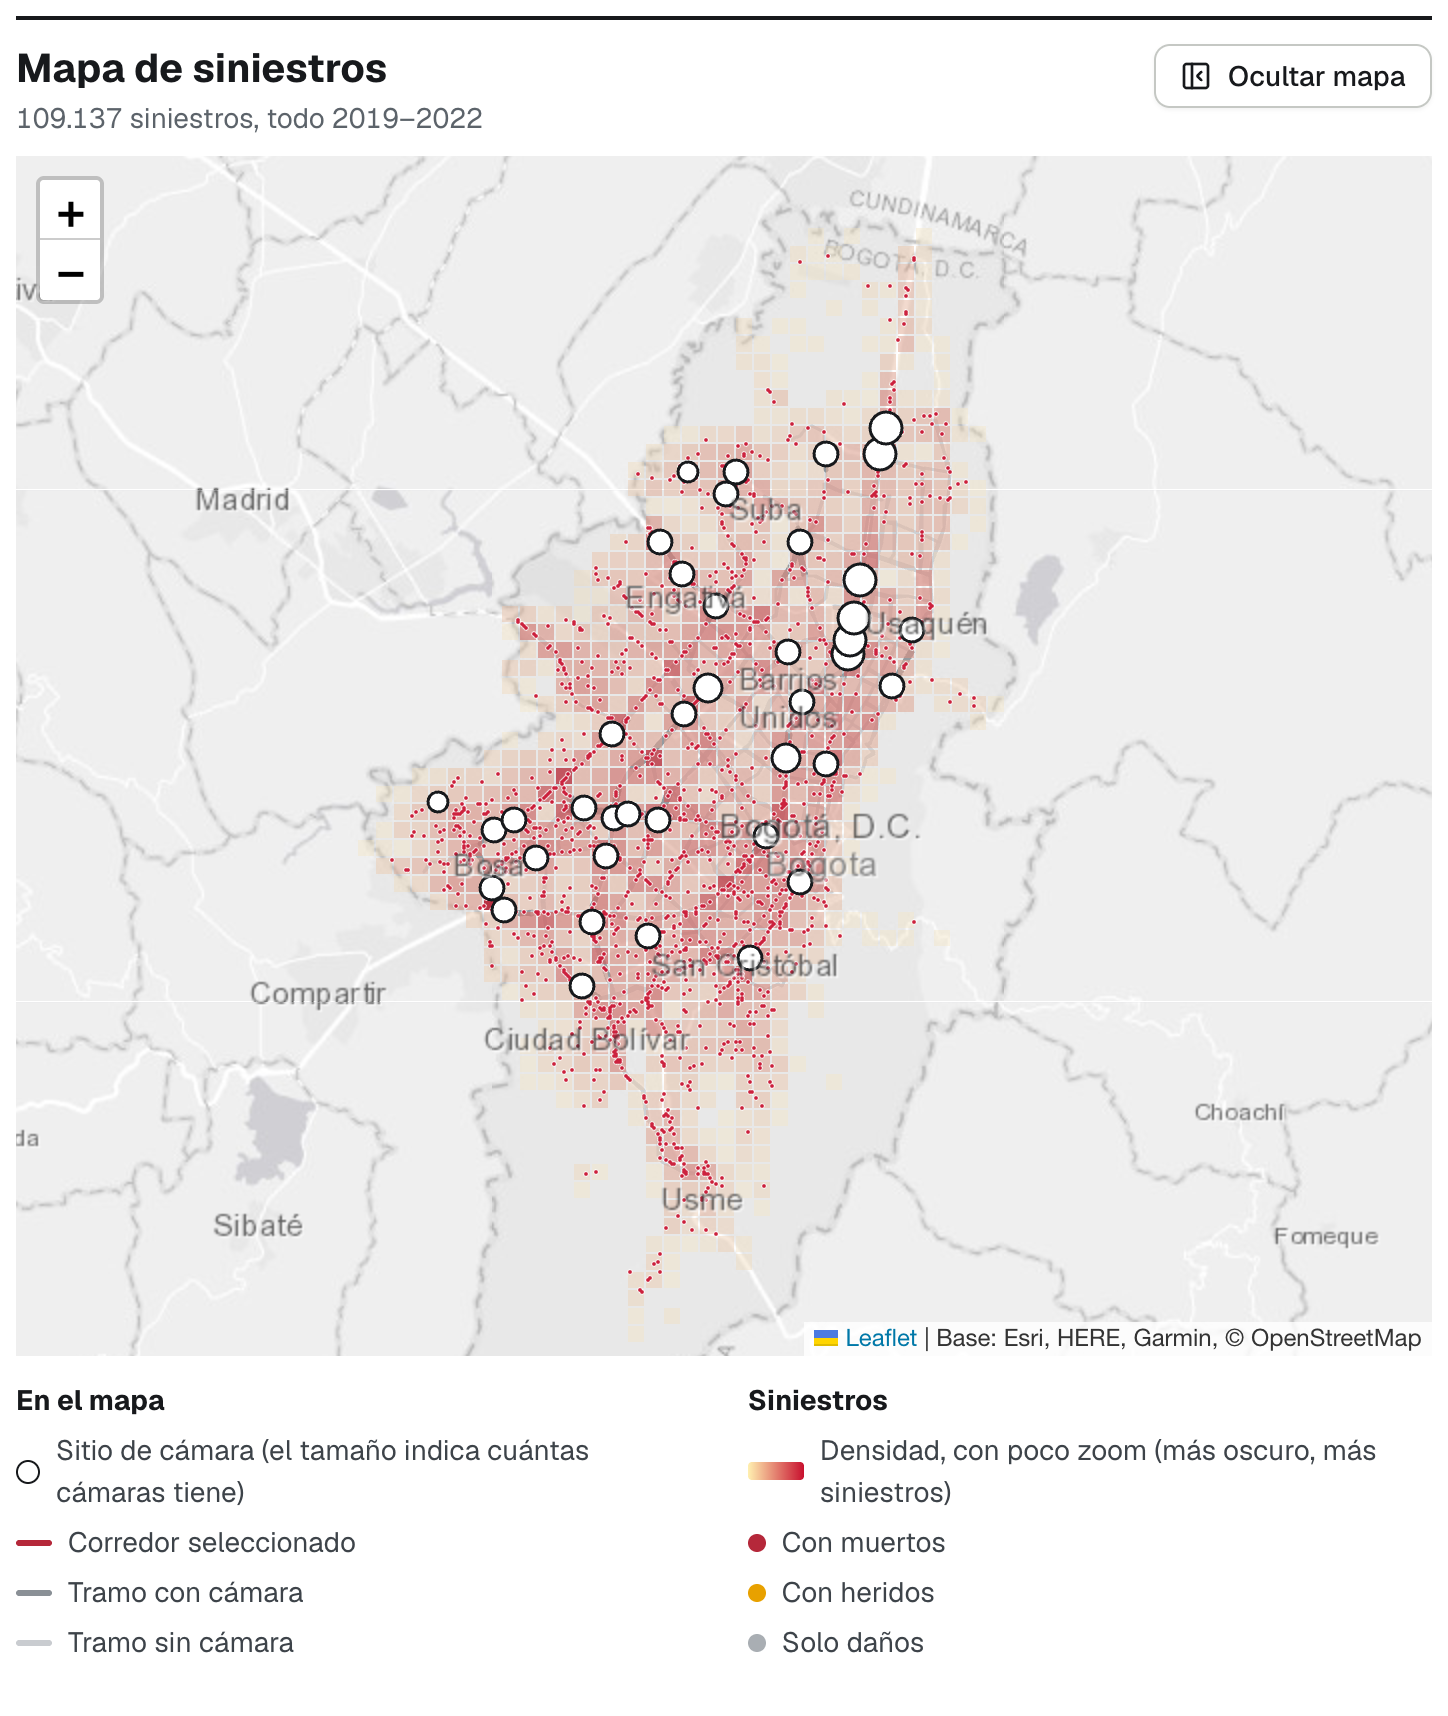
\includegraphics[width=0.55\linewidth,height=0.4\textheight,keepaspectratio]{i_mapa}
\caption{Mapa de densidad con los sitios de cámara y su leyenda}
\end{figure}

La pregunta de si bajó más donde hay cámara la respondemos con dos barras de cambio porcentual que parten de un mismo cero, una para la zona con cámara y otra para las vías sin cámara. Al principio teníamos barras de antes y después con una escala distinta para cada zona, de manera que las longitudes no se podían comparar y el resultado quedaba escondido en una frase. Con la escala común la comparación se hace a simple vista, debajo de cada barra quedan las cifras en siniestros por mes para quien necesite citarlas y la diferencia entre ambos cambios aparece escrita, que es justamente lo que Carolina lleva a una discusión sobre el programa.

\begin{figure}[H]\centering
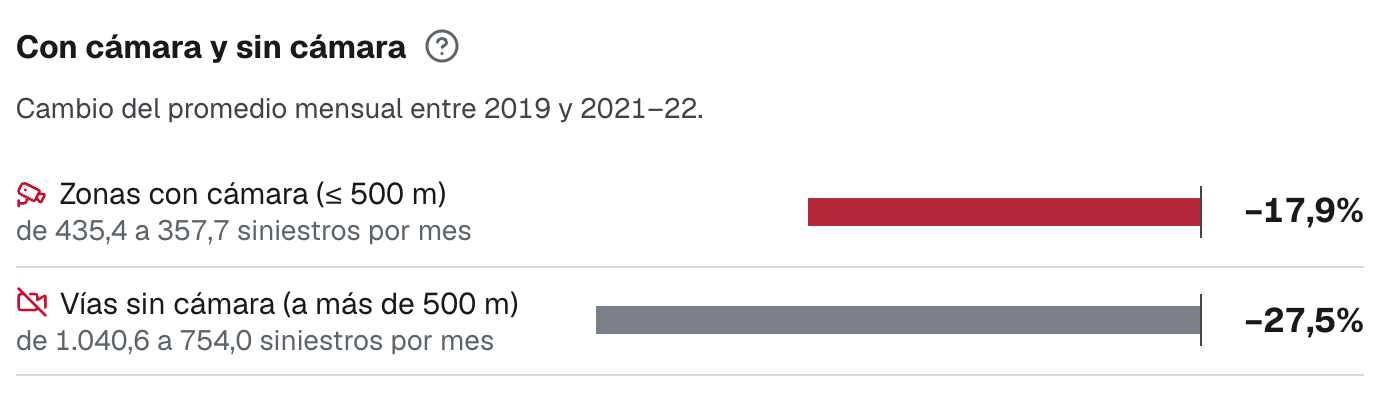
\includegraphics[width=0.7\linewidth,height=0.2\textheight,keepaspectratio]{i_cambio}
\caption{Barras de cambio con y sin cámara sobre una escala común}
\end{figure}

Junto a ese cambio dejamos los siniestros por año en barras verticales, porque son pocos periodos ordenados y la altura permite ver de inmediato la caída de 2020 y cuánto se recuperó después, lo que evita que alguien lea el cambio con y sin cámara como si no hubiera pasado nada más en la ciudad. Los colores separan el antes, la transición y el después y se repiten en el resto del dashboard, así que quien aprende a leerlos aquí no tiene que volver a hacerlo en otra vista. Para las víctimas usamos barras pareadas por condición, que comparan la distribución entre los dos periodos con la cifra al final de cada barra y el cambio porcentual alineado a la derecha, de modo que se puede recorrer la columna de porcentajes para encontrar qué grupo subió y cuál bajó.

\begin{figure}[H]\centering
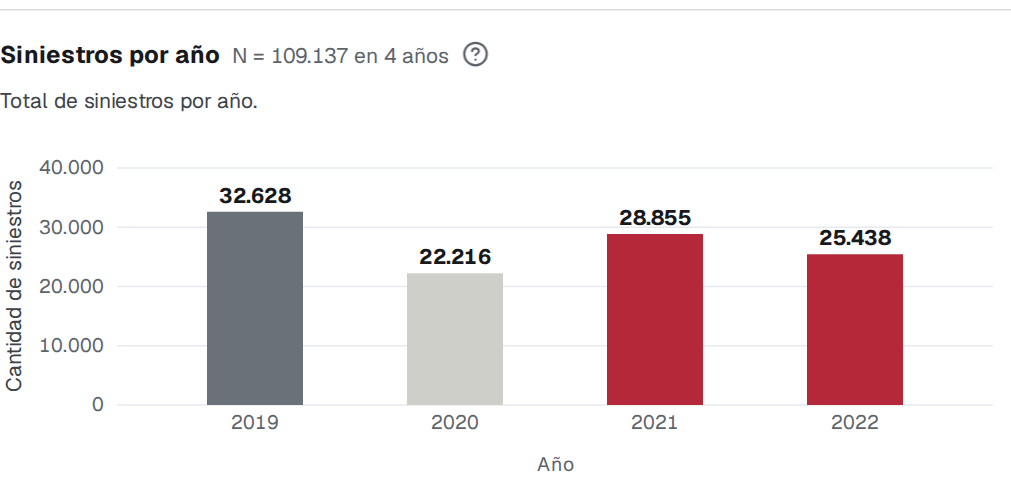
\includegraphics[width=0.49\linewidth,height=0.26\textheight,keepaspectratio]{i_anual}\hfill
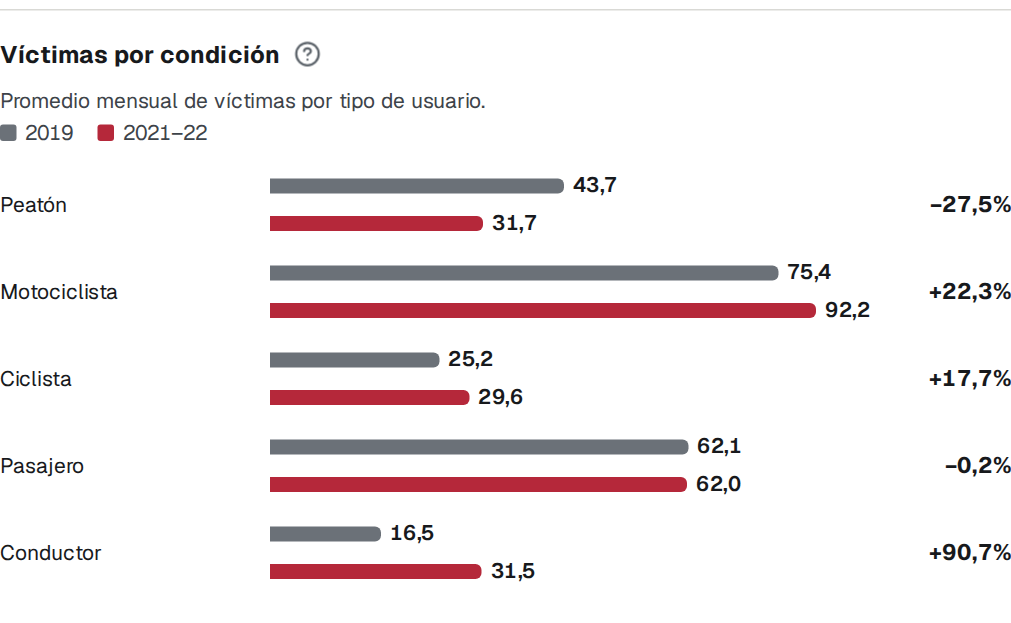
\includegraphics[width=0.49\linewidth,height=0.26\textheight,keepaspectratio]{i_victimas}
\caption{Siniestros por año y víctimas por condición}
\end{figure}

\subsection{Idioms para el tiempo}

Para saber cuándo cambia la tendencia usamos una línea mensual, porque el tiempo es ordenado y la pendiente deja ver subidas y bajadas que en barras separadas costaría seguir. La línea va acompañada del promedio de 2019 como referencia, de la marca de las multas y de una cinta junto al eje con la pandemia y la instalación, que le dan al lector el contexto sin tapar los datos. Debajo hay una franja con toda la serie que funciona como vista de conjunto, de modo que Andrés puede arrastrar sobre unos meses para acercarse y seguir sabiendo en qué parte de los cuatro años está parado.

\begin{figure}[H]\centering
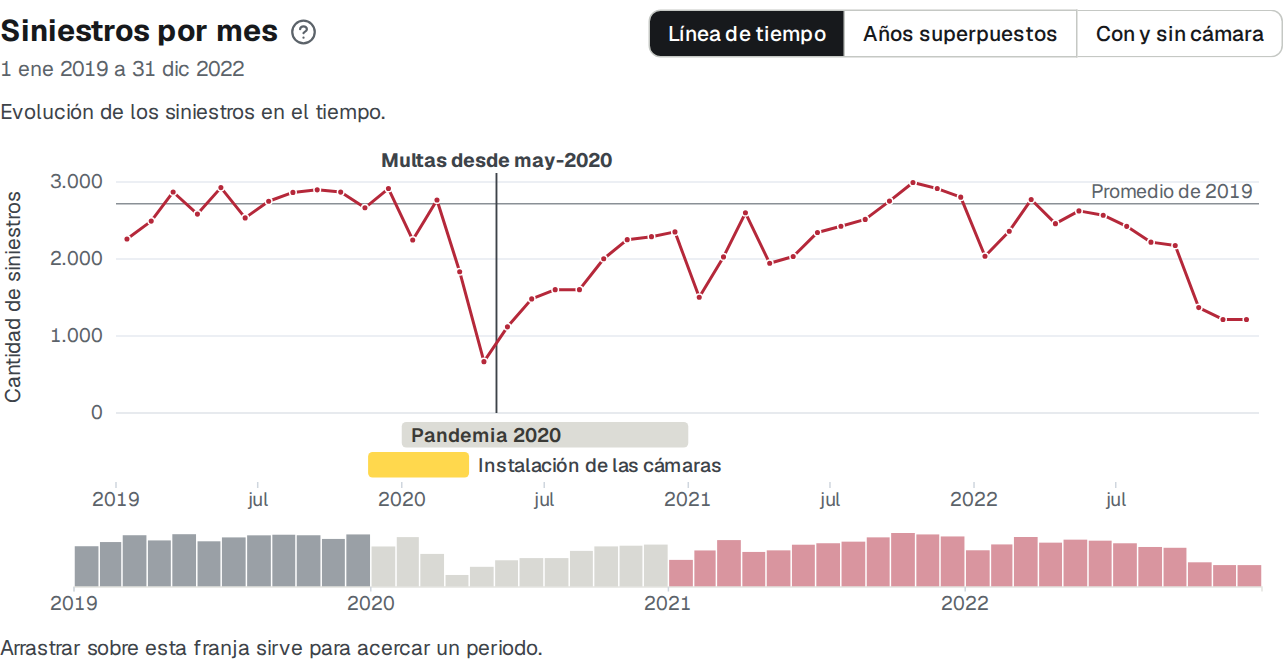
\includegraphics[width=0.8\linewidth,height=0.28\textheight,keepaspectratio]{i_serie}
\caption{Serie mensual con referencia, periodos marcados y franja para acercar}
\end{figure}

Cuando lo que se quiere es comparar un año con otro usamos recuadros pequeños, uno por año, con la misma escala y con 2019 en gris detrás de cada uno. Empezamos superponiendo las cuatro líneas en una sola gráfica, pero se cruzaban y había que seguirlas con el dedo para saber cuál era cuál, mientras que con los recuadros la comparación se hace por posición y cada año se lee contra la misma referencia, que es el último año antes de las cámaras.

\begin{figure}[H]\centering
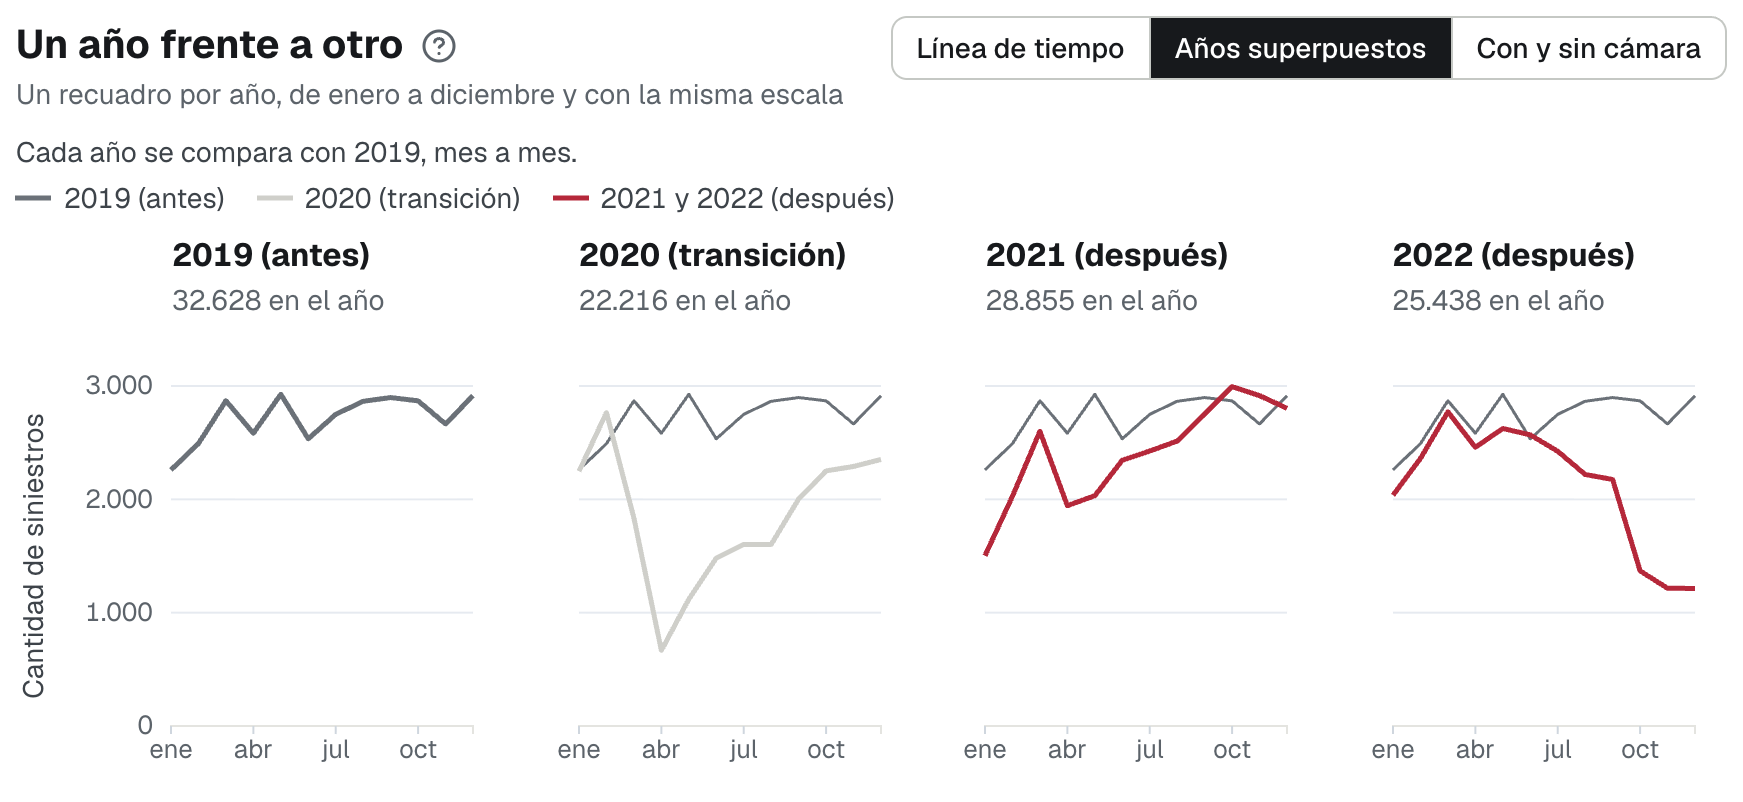
\includegraphics[width=0.8\linewidth,height=0.22\textheight,keepaspectratio]{i_anios}
\caption{Un recuadro por año, con 2019 como referencia}
\end{figure}

Para comparar la evolución con y sin cámara las dos series se expresan como porcentaje de su propio nivel de 2019, porque sus volúmenes son tan distintos que en la misma escala una aplastaría a la otra. Como las dos líneas quedan muy cerca, debajo graficamos la resta en un área que cambia de color según quién está más alto, que es el dato derivado que de verdad interesa, y así nadie tiene que calcular a ojo la distancia entre dos líneas casi iguales. La instalación, la pandemia y las multas se marcan igual que en la serie para que la lectura sea la misma.

\begin{figure}[H]\centering
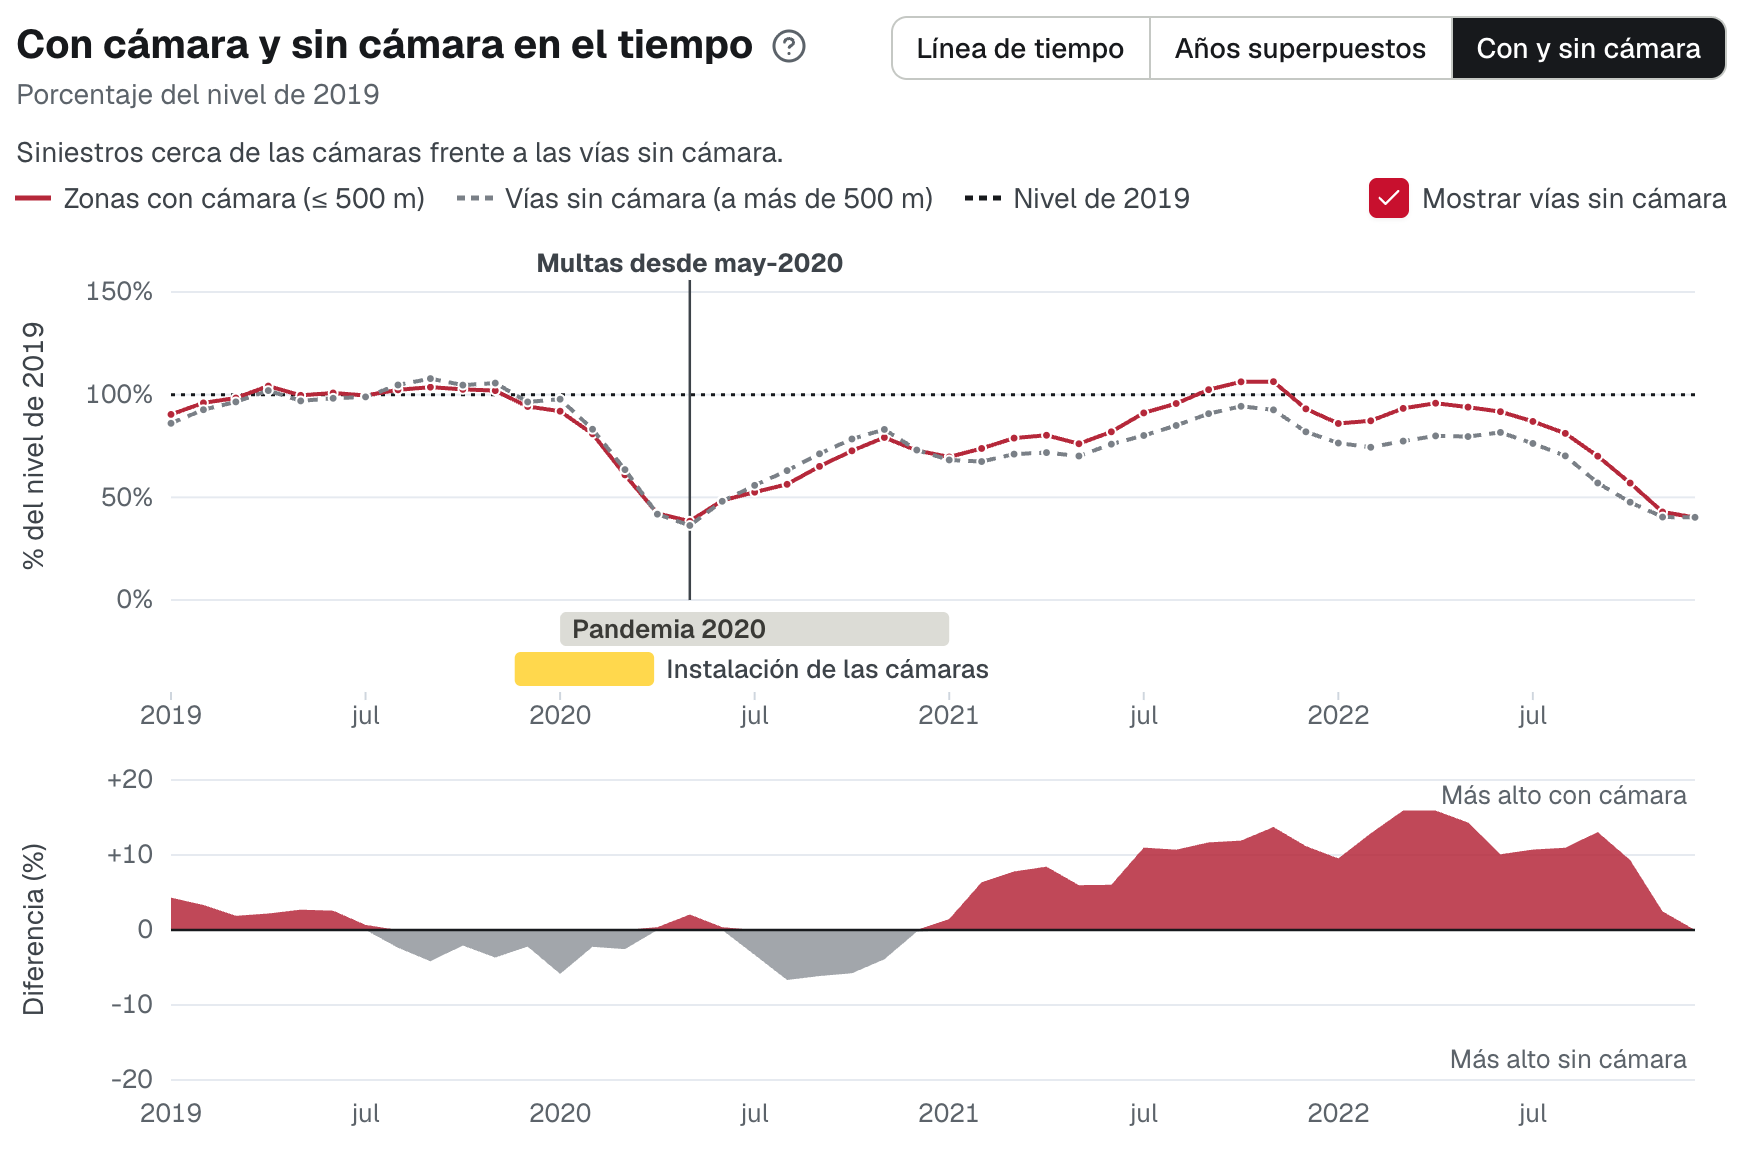
\includegraphics[width=0.75\linewidth,height=0.32\textheight,keepaspectratio]{i_indice}
\caption{Series indexadas a 2019 y área de diferencia}
\end{figure}

La velocidad del tráfico sigue la misma lógica, con las líneas del percentil 85 en km/h, que conservan el valor real y se pueden leer contra el límite del sitio, y debajo la diferencia entre los tramos con y sin cámara. La dejamos en gráficas aparte en lugar de ponerla sobre los siniestros con un doble eje, porque dos escalas en una misma gráfica sugieren relaciones que no existen. Para Diana esto responde a qué velocidad se circula en su ruta, y para Carolina muestra si el tráfico se hizo más lento donde se puso la cámara.

\begin{figure}[H]\centering
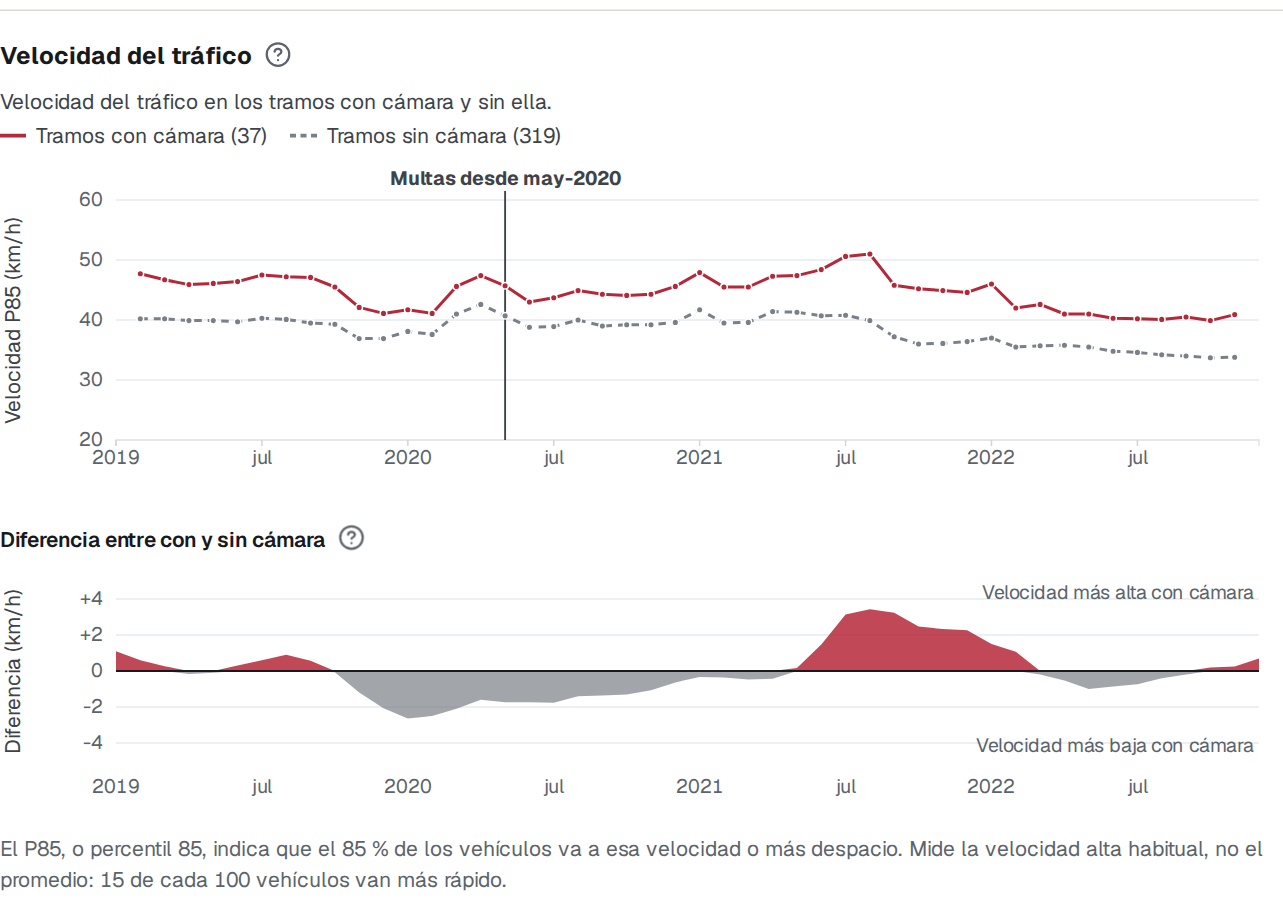
\includegraphics[width=0.75\linewidth,height=0.32\textheight,keepaspectratio]{i_velocidad}
\caption{Velocidad P85 y diferencia entre tramos con y sin cámara}
\end{figure}

\subsection{Idioms para corredores y meses}

Para encontrar el corredor que más mejora o empeora usamos una lista ordenada con barras divergentes centradas en la referencia, de manera que los extremos quedan arriba y abajo y el lado de la barra dice si el corredor tuvo menos o más casos que las vías sin cámara. Cada fila trae además una miniatura de su serie mensual con la instalación sombreada, que permite ver si el cambio fue sostenido o producto de unos pocos meses sin abrir el detalle, y los corredores con pocos siniestros se señalan para que Andrés no construya una noticia sobre un porcentaje inestable.

\begin{figure}[H]\centering
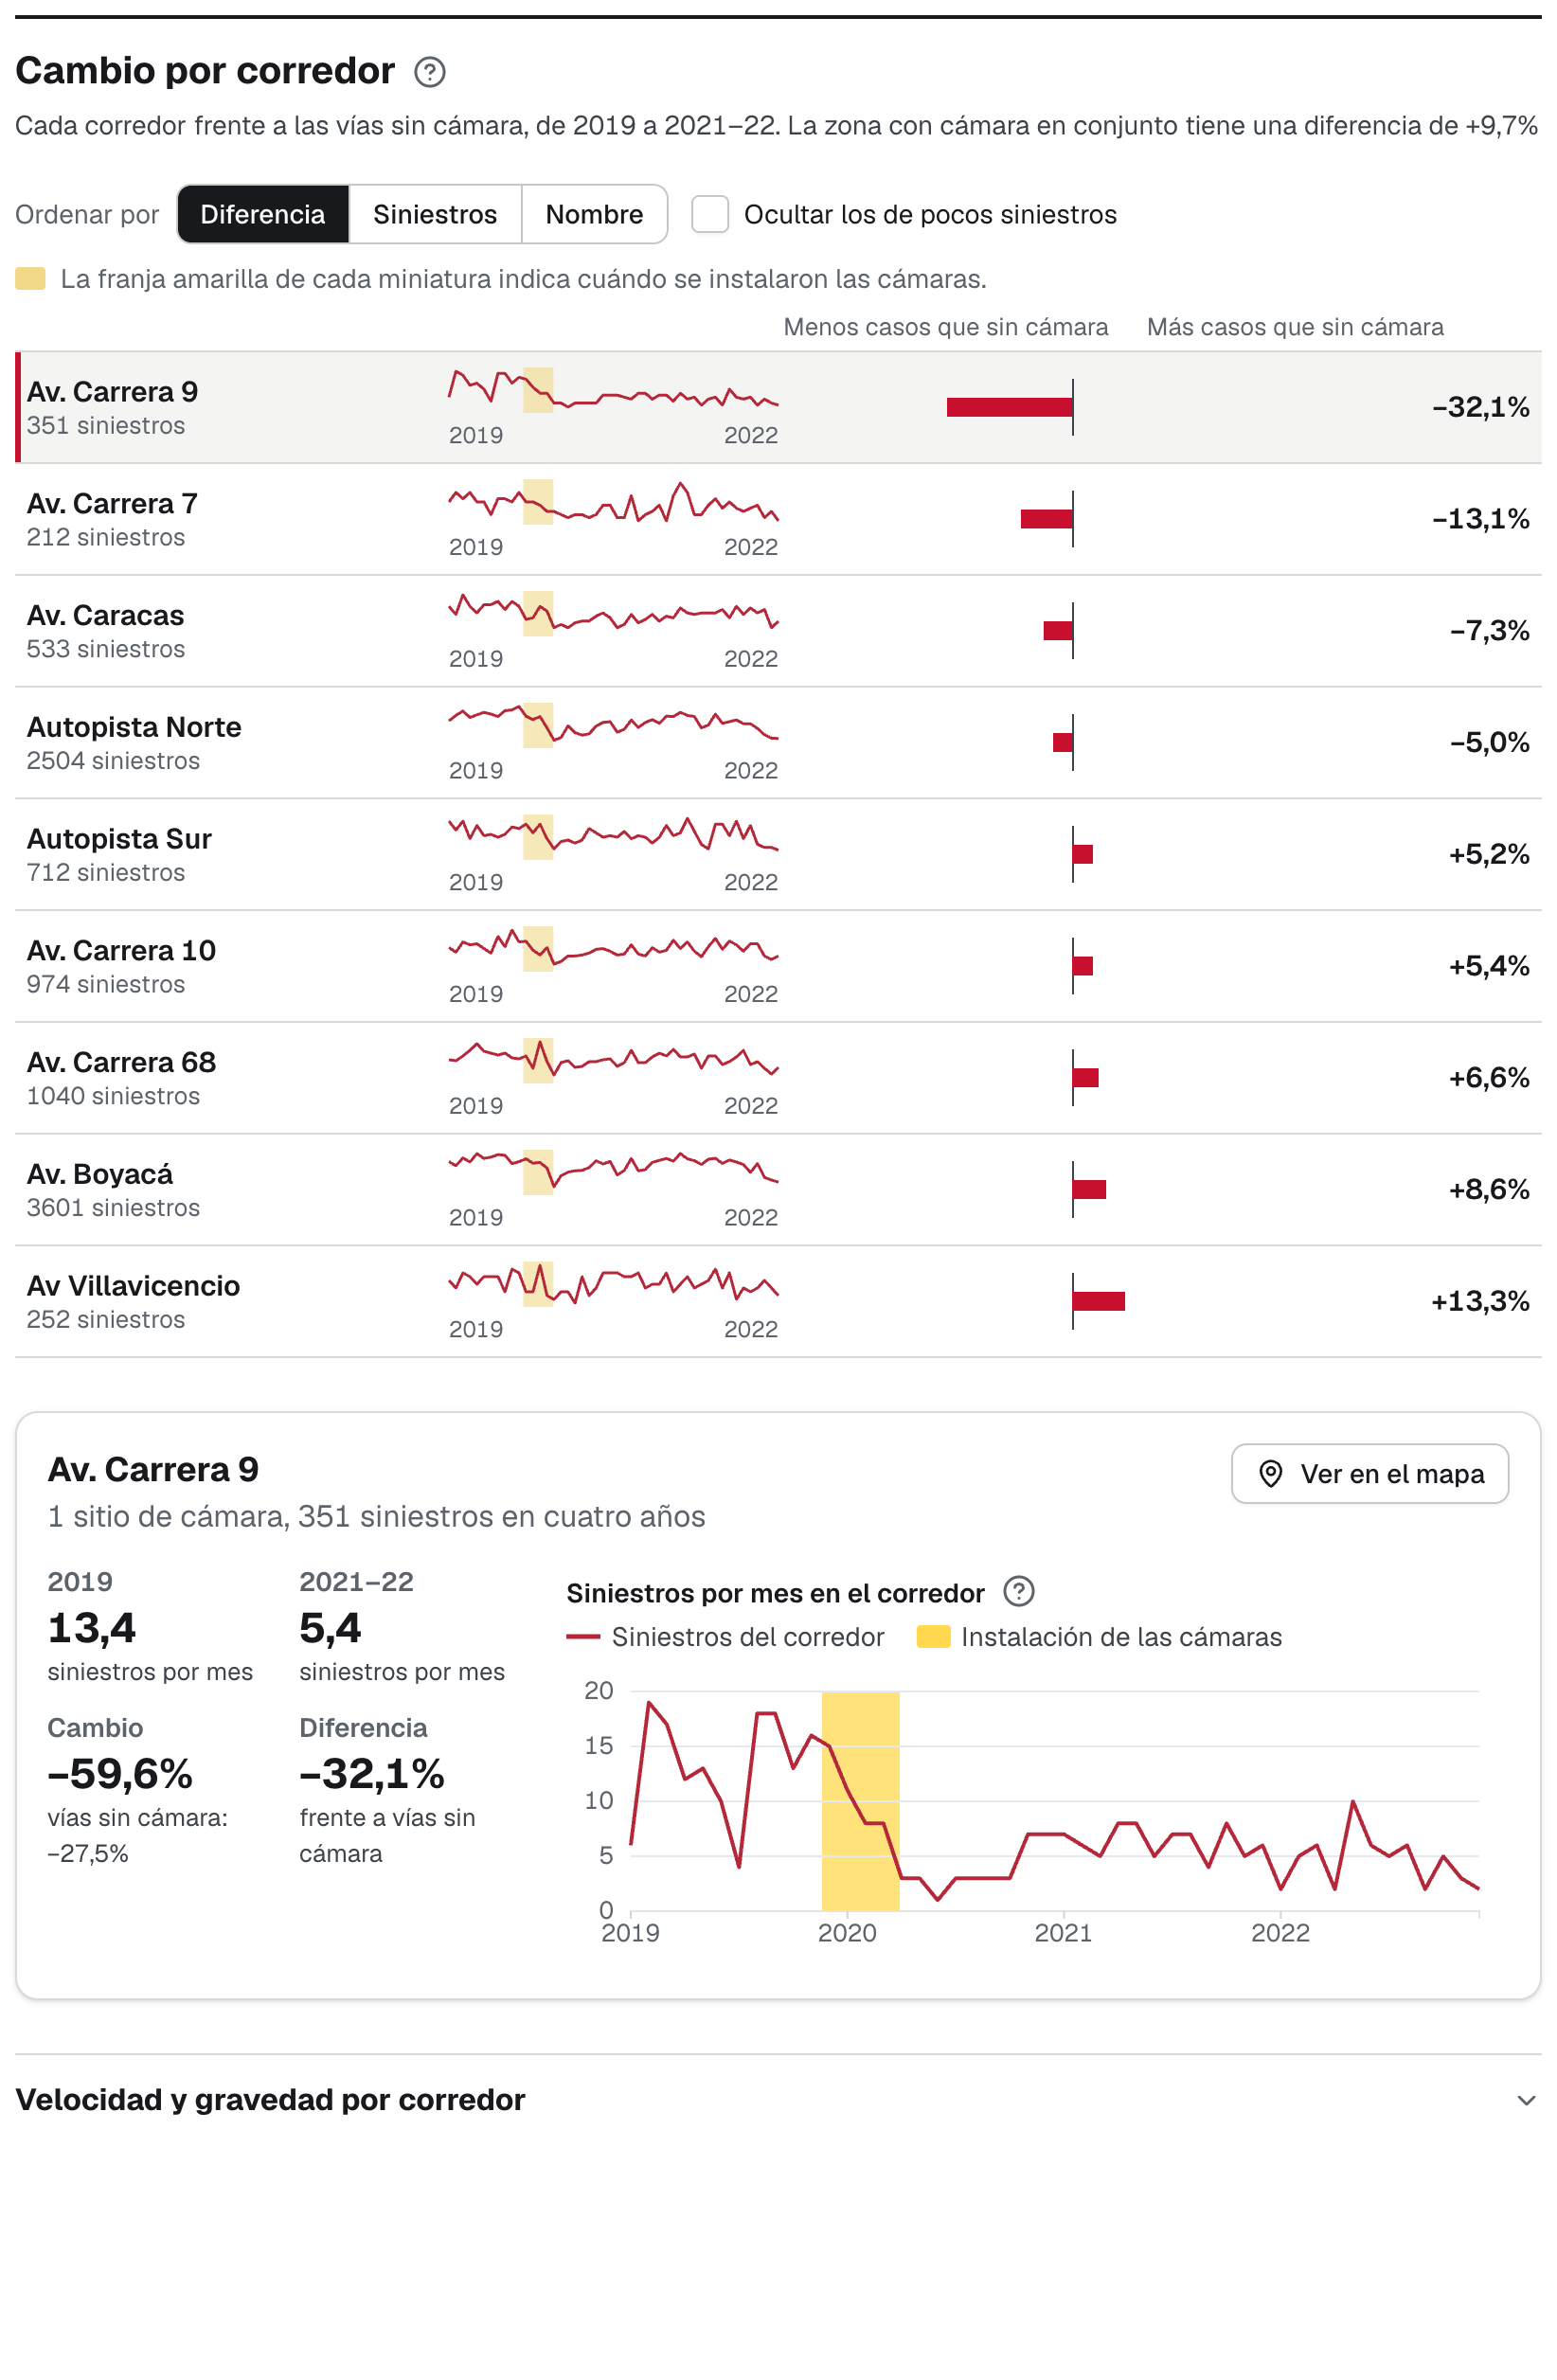
\includegraphics[width=0.8\linewidth,height=0.34\textheight,keepaspectratio]{i_corredores}
\caption{Lista de corredores con barras divergentes y miniaturas}
\end{figure}

Al elegir un corredor se abre una tarjeta con las cifras de cada periodo, el cambio, la diferencia frente a las vías sin cámara y su serie con más tamaño. Cada número lleva su unidad escrita debajo, porque en una versión anterior un valor suelto no decía qué se estaba contando. La relación entre velocidad y gravedad la mostramos en un gráfico de dispersión con un punto por corredor, que es el idiom que deja ver si dos variables se mueven juntas y cuáles corredores se salen del grupo, y queda plegado porque responde una pregunta secundaria.

\begin{figure}[H]\centering
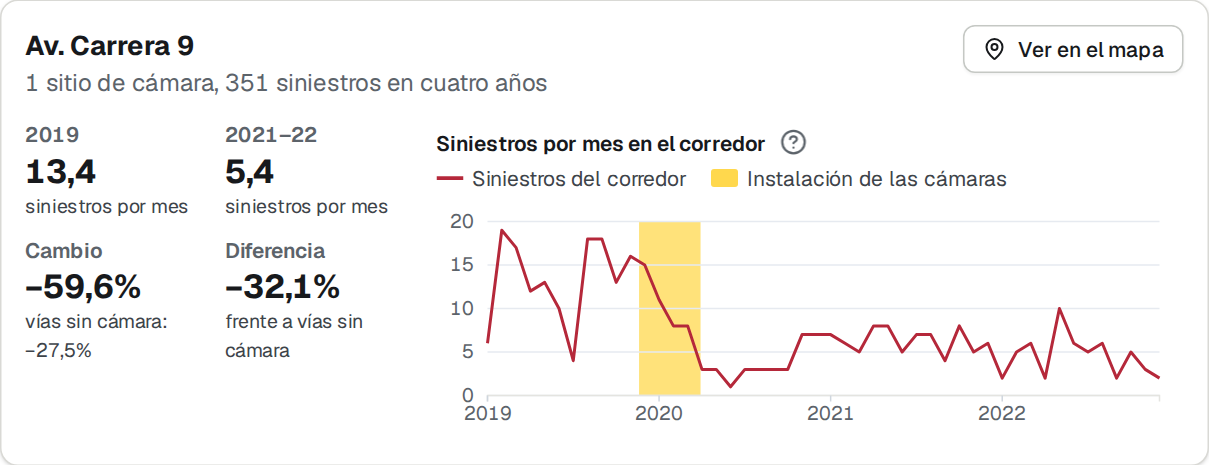
\includegraphics[width=0.75\linewidth,height=0.22\textheight,keepaspectratio]{i_detalle}
\caption{Tarjeta de detalle de un corredor}
\end{figure}
\begin{figure}[H]\centering
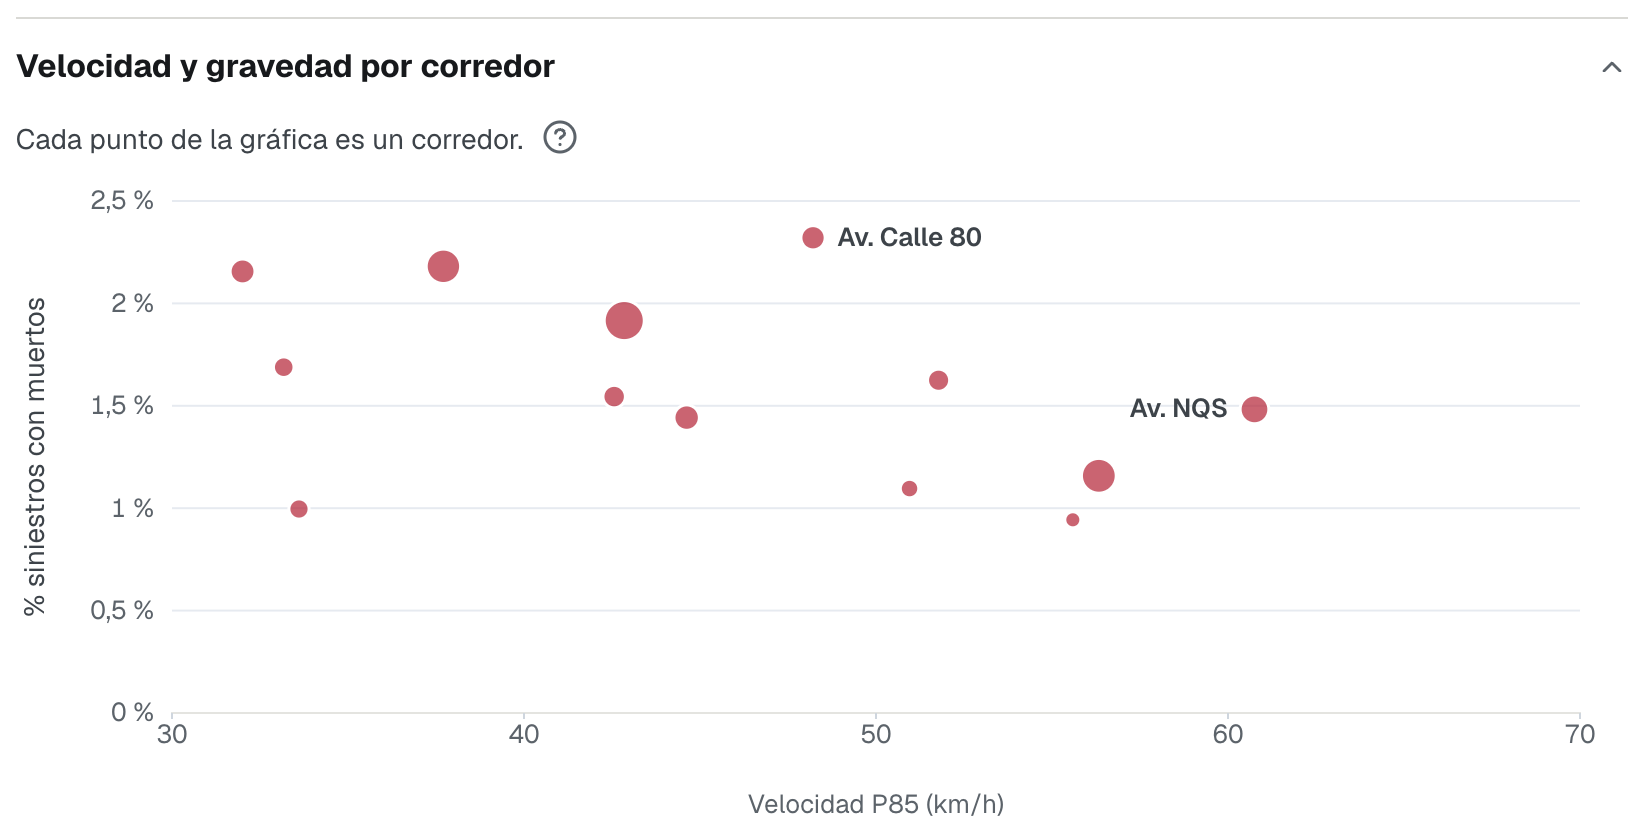
\includegraphics[width=0.65\linewidth,height=0.25\textheight,keepaspectratio]{i_dispersion}
\caption{Dispersión de velocidad y gravedad por corredor}
\end{figure}

La comparación de meses usa una barra por mes, que se pinta según el grupo al que pertenece, y una tabla debajo con el promedio mensual de cada grupo y el cambio entre ellos. Las barras sirven para elegir y para ver qué tan parecidos son los meses dentro de un grupo, y la tabla sirve para leer cifras exactas de siniestros, víctimas, cámaras instaladas y velocidad, que en una sola gráfica no cabrían sin mezclar unidades. Con esto Carolina puede armar su propio antes y después, por ejemplo dejando por fuera la pandemia, sin pedirle a nadie un cruce nuevo.

\begin{figure}[H]\centering
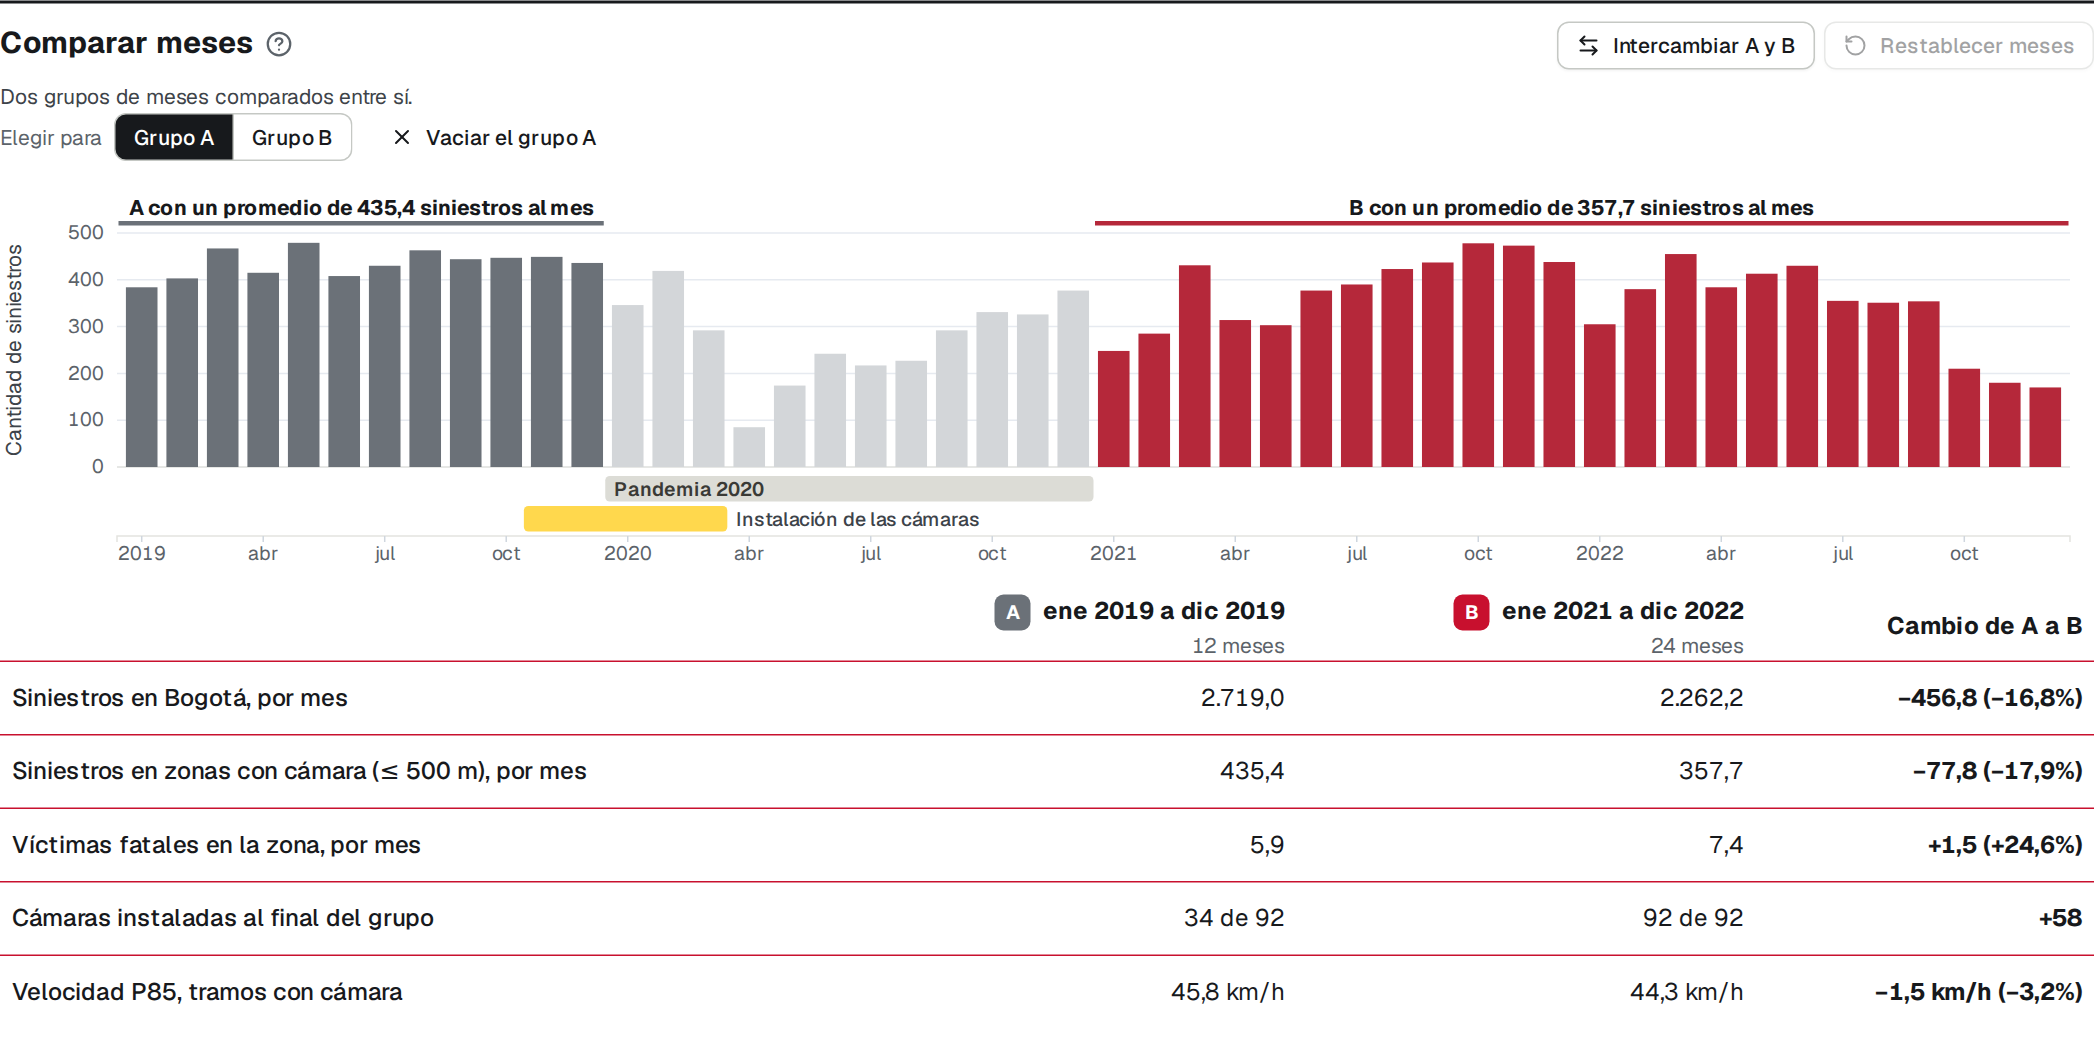
\includegraphics[width=0.85\linewidth,height=0.38\textheight,keepaspectratio]{i_ab}
\caption{Comparar meses, con las barras para elegir y la tabla de promedios}
\end{figure}

\subsection{Marcas y canales}

La siguiente tabla resume cómo codificamos cada dato, y la intención fue que un mismo canal signifique lo mismo en todas las vistas para que lo aprendido en una sirva en las demás.

\begin{table}[H]\centering\small
\begin{tabularx}{\linewidth}{P{3.6cm}P{4.4cm}L}
\toprule
\textbf{Dato} & \textbf{Marca y canal} & \textbf{Razón}\\
\midrule
Ubicación & Puntos por posición en el mapa & Es el canal natural para datos espaciales.\\
Cámaras por sitio & Tamaño del círculo & Es una magnitud ordenada y no necesita precisión.\\
Densidad & Rampa de amarillo a rojo & Con poco zoom los puntos se tapan.\\
Gravedad & Rojo, ámbar y gris & Se lee como un orden de severidad.\\
Con y sin cámara & Rojo continuo y gris punteado & Dos canales, para no depender solo del color.\\
Antes, 2020 y después & Gris, gris claro y rojo & El mismo significado en todas las vistas.\\
Cambio porcentual & Longitud desde un cero común & Es de los canales más precisos para comparar.\\
Instalación y pandemia & Cinta junto al eje & Da contexto sin tapar los datos.\\
\bottomrule
\end{tabularx}
\caption{Marcas y canales}
\end{table}

El rojo y el amarillo vienen de la bandera de Bogotá, y el rojo señala lo observado, es decir, lo que ocurrió después y cerca de las cámaras, sin ser un juicio de bueno o malo. Reservamos ese rojo para los datos y las acciones principales y dejamos los controles seleccionados en tinta oscura, porque si todo lo activo fuera rojo se perdería la señal de qué es lo que se está comparando. En las escalas buscamos que lo comparable comparta eje, mientras que las miniaturas de los corredores tienen escala propia porque allí interesa la forma de la serie y su tamaño ya está en las cifras de la fila.

\subsection{Manipulación mediante filtros e interacción}

Los filtros salen de las preguntas y de los perfiles, y cada uno existe porque cambia la respuesta de alguna de ellas, de modo que no pusimos un control por cada columna disponible para no abrir combinaciones que dejan muy pocos siniestros.

\begin{table}[H]\centering\small
\begin{tabularx}{\linewidth}{P{3.3cm}P{4.2cm}L}
\toprule
\textbf{Filtro} & \textbf{Opciones} & \textbf{Por qué lo incluimos}\\
\midrule
Corredor & Los 18 o toda la ciudad & Es la forma en que se habla de una vía y lo que Andrés y Diana buscan. Tiene búsqueda para no recorrer la lista.\\
Sitio de cámara & Los 40 sitios & Carolina quiere el antes y después por cámara. Depende del corredor elegido para acortar las opciones.\\
Periodo & Todo, antes, 2020 y después & Permite aislar la transición y ver dónde ocurren los siniestros en cada momento.\\
Gravedad & Todos, heridos, heridos o muertos y muertos & Un programa de cámaras se juzga por las muertes, pero los fatales son pocos, así que los niveles dejan pasar de lo más frecuente a lo más grave.\\
Tipo de siniestro & Seis clases & La pregunta de tendencia habla de choques fatales y no de cualquier siniestro fatal.\\
Actor involucrado & Once marcas & Sirve para mirar motos, peatones o embriaguez, y salió de los comentarios del paper prototype.\\
Radio & 150 a 1.000 m & Deja probar el supuesto de qué es cerca.\\
Excluir intersecciones ambiguas & Sí o no & Evita atribuir a un corredor lo que pudo ocurrir en el que lo cruza.\\
Siniestros en el corredor & Casilla en el mapa & Responde la duda de si se toma toda la vía o solo el tramo de la cámara.\\
\bottomrule
\end{tabularx}
\caption{Filtros y su razón}
\end{table}

Dejamos a la vista los cuatro primeros porque son los que usa cualquier perfil y escondimos el resto en ``Más filtros'', pensando en que Diana necesita pocos controles. Al abrir, la gravedad está en Todos y el radio en 500 metros para que lo primero que se ve sea el panorama completo, y unas etiquetas recuerdan el alcance activo, incluidos los filtros escondidos. Los selectores de corredor y de sitio tienen búsqueda, porque recorrer una lista de 40 sitios a ojo es lento, y si un filtro no cambia una vista no se muestra en ella, como el periodo en Comparar meses, donde los meses se eligen en la gráfica.

\begin{figure}[H]\centering
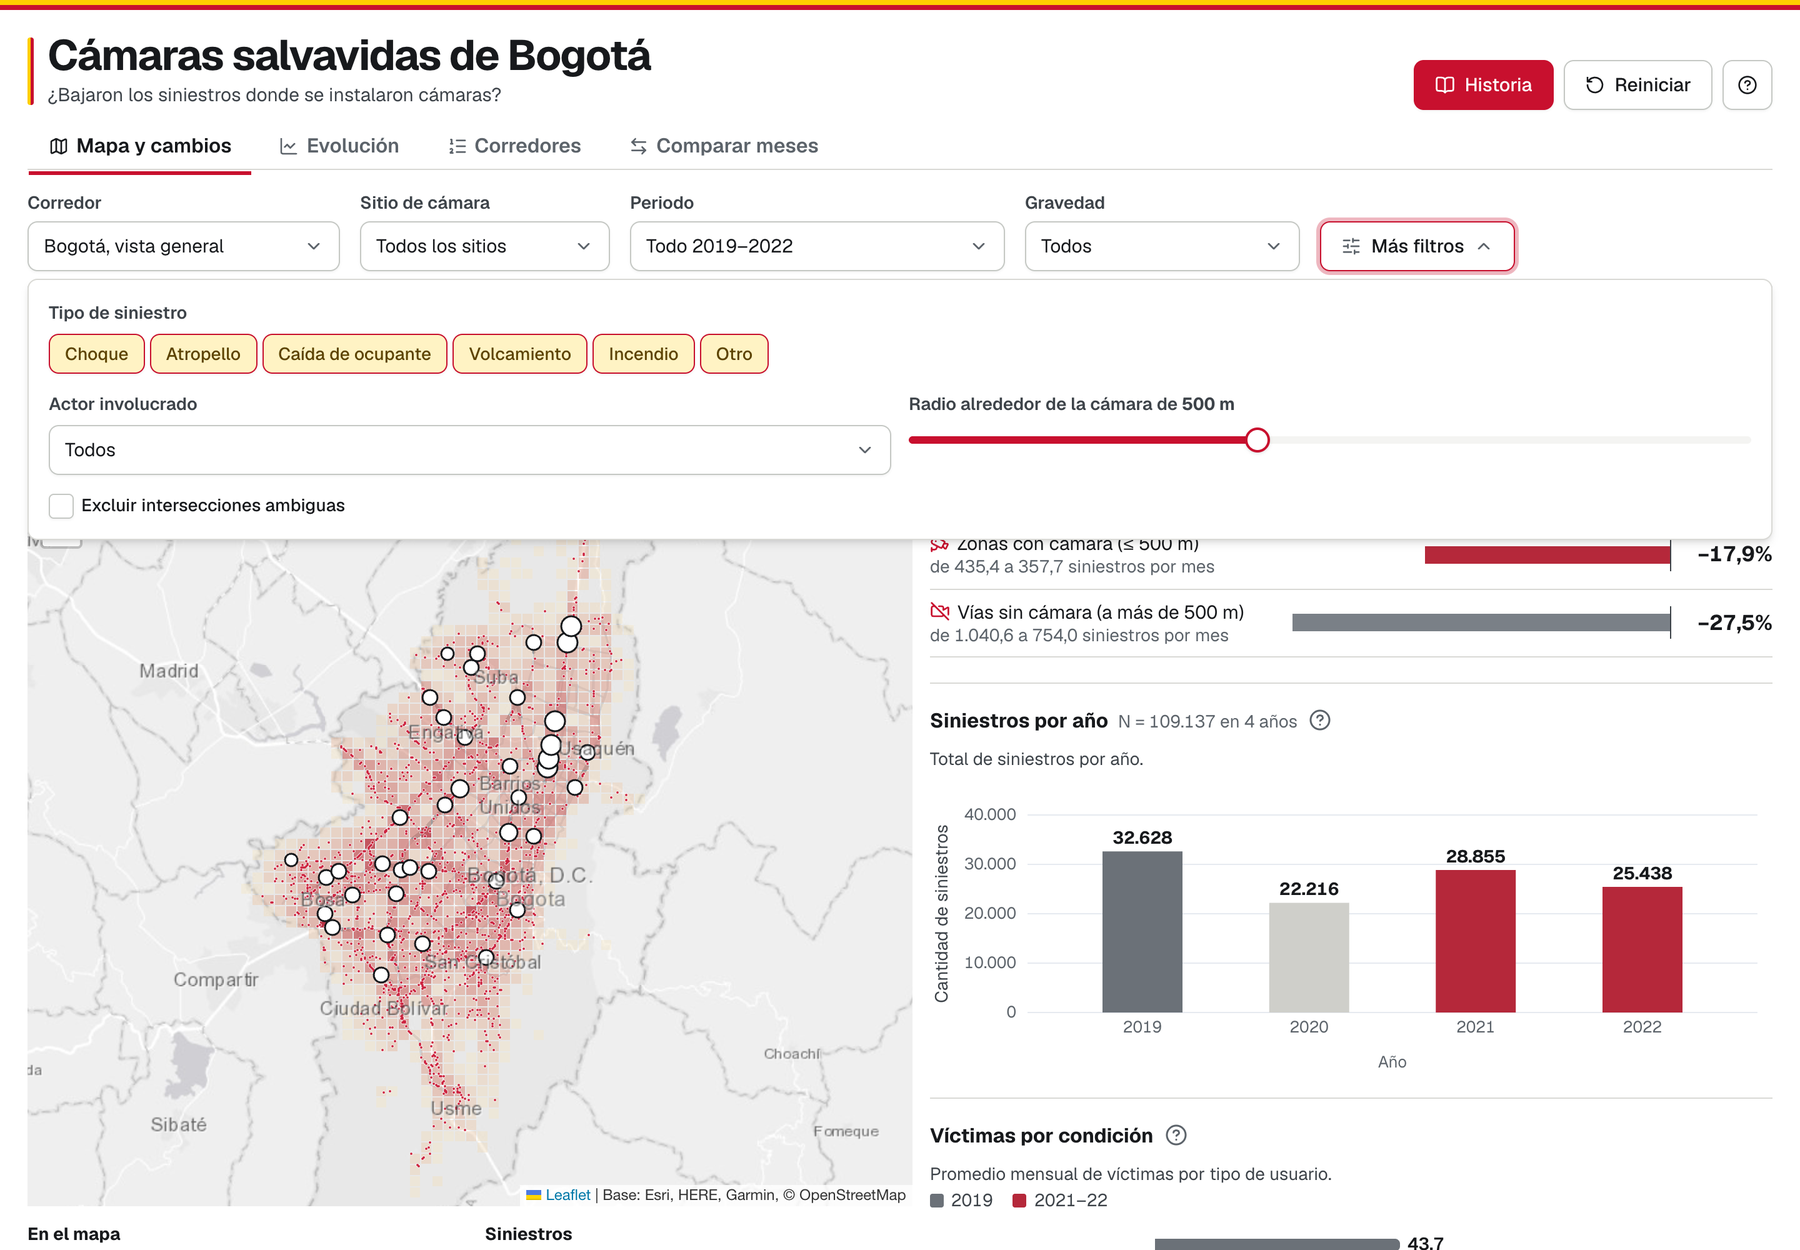
\includegraphics[width=0.49\linewidth,height=0.3\textheight,keepaspectratio]{f_mas}\hfill
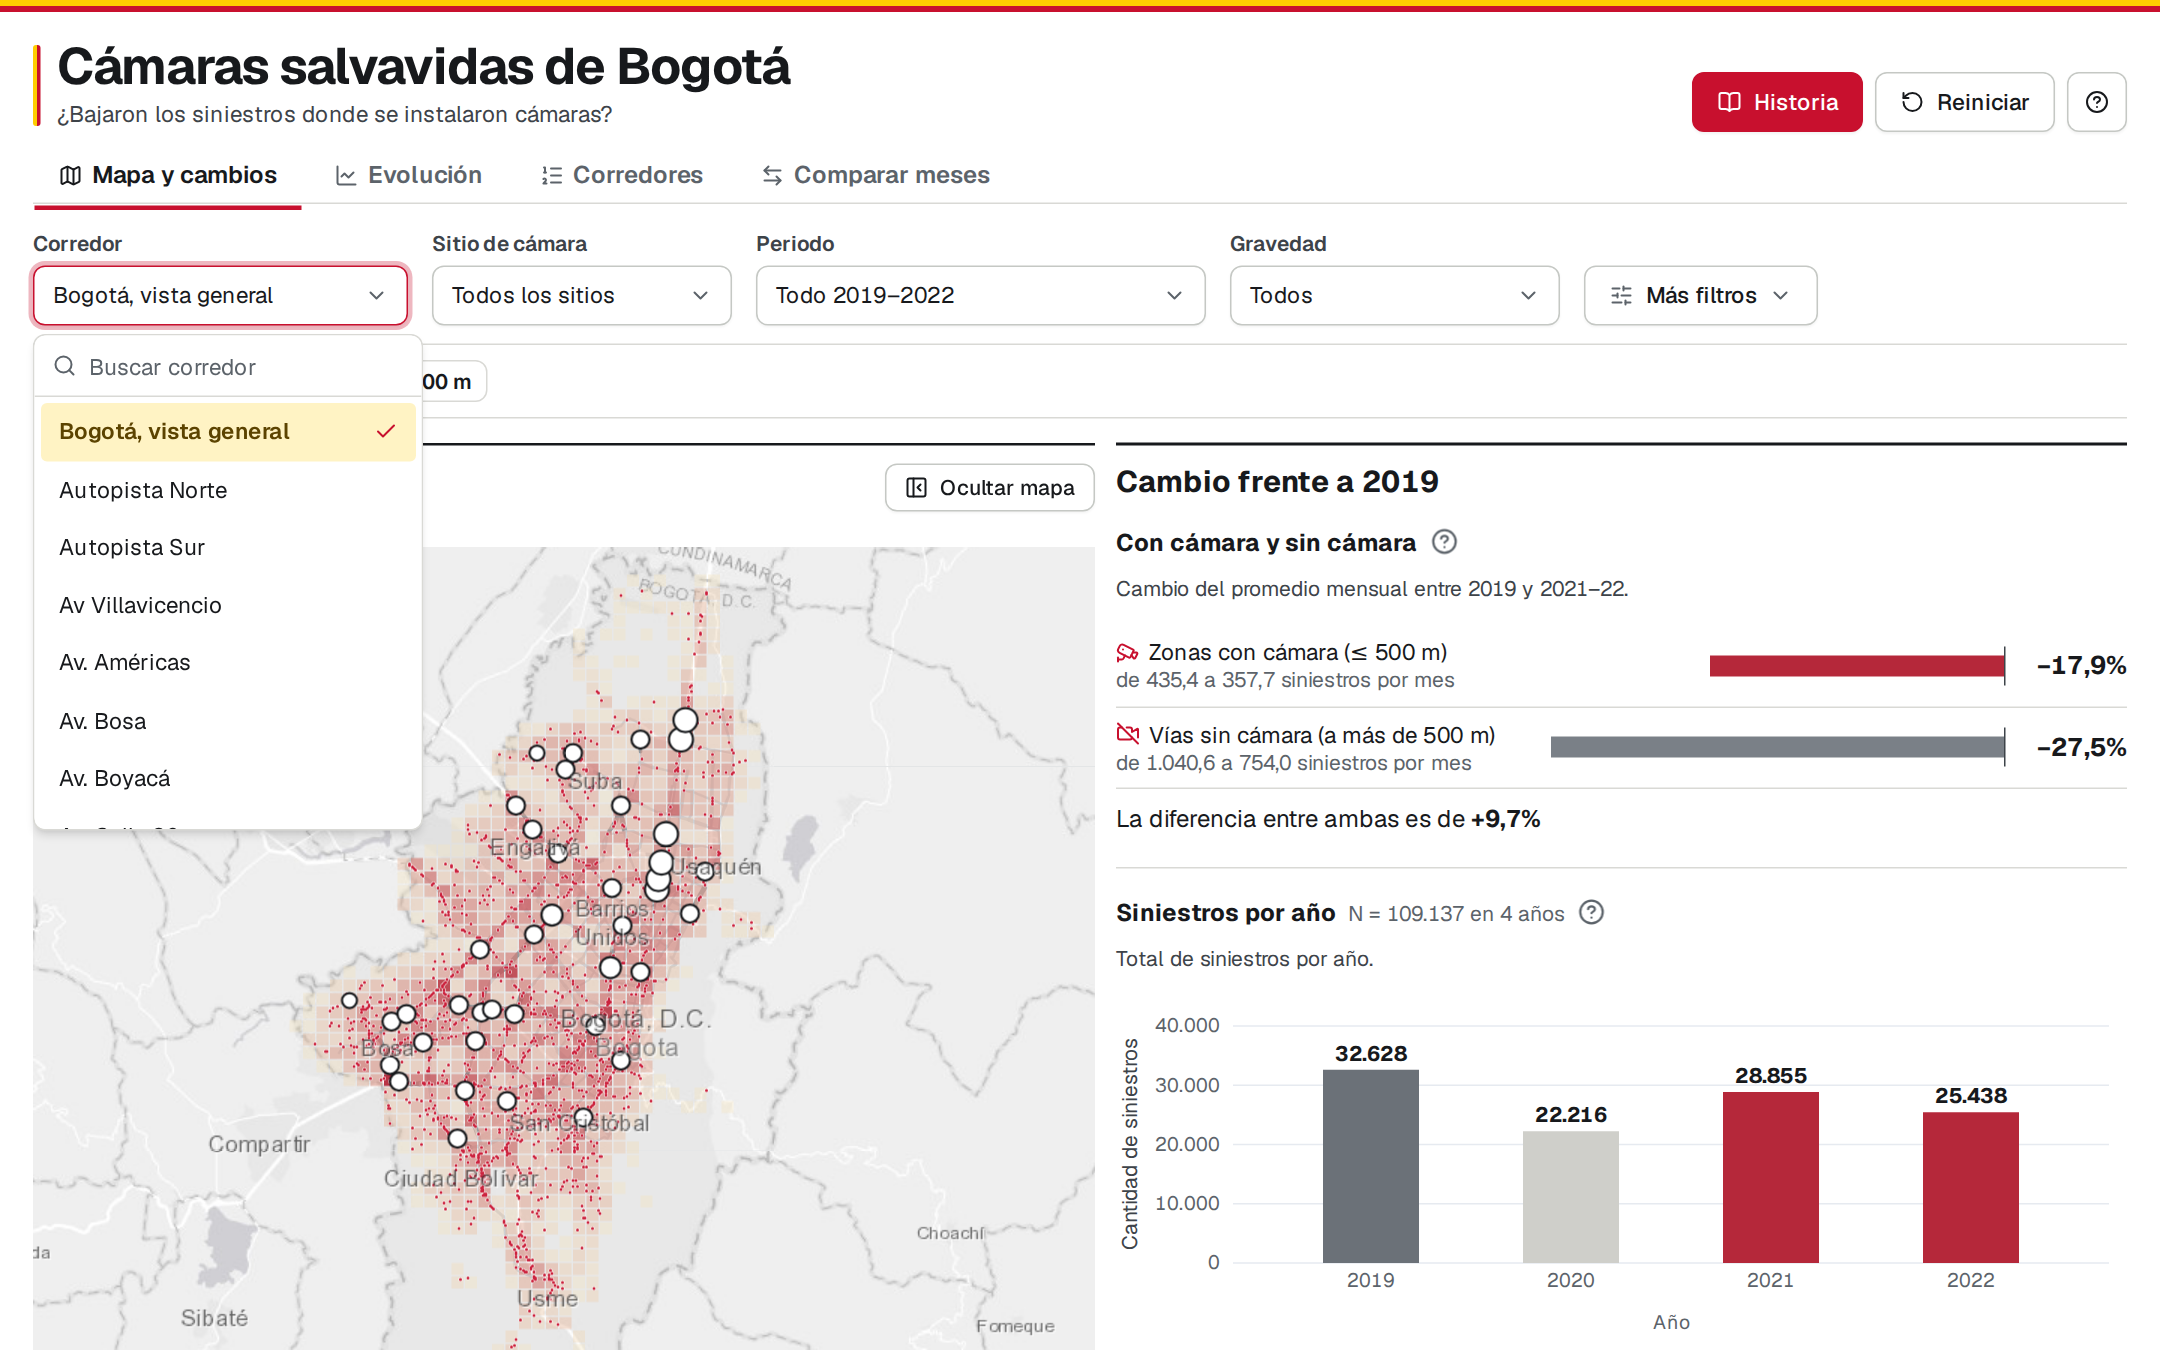
\includegraphics[width=0.49\linewidth,height=0.3\textheight,keepaspectratio]{f_buscar}
\caption{Filtros adicionales y búsqueda de corredor}
\end{figure}

La selección se puede hacer desde el menú o con un clic en el mapa, porque unas personas conocen el nombre de la vía y otras reconocen el lugar, y se conserva al cambiar de pestaña para no tener que repetirla. Al elegir un sitio el mapa se acerca, dibuja el radio y rotula la cámara, y las cifras, las series y la velocidad pasan a referirse a ese lugar, que es lo que Carolina pide cuando habla del antes y después por cámara. La casilla del corredor amplía los puntos a toda la vía sin cambiar la comparación con y sin cámara, y respondió una duda que nos plantearon en el paper prototype.

\begin{figure}[H]\centering
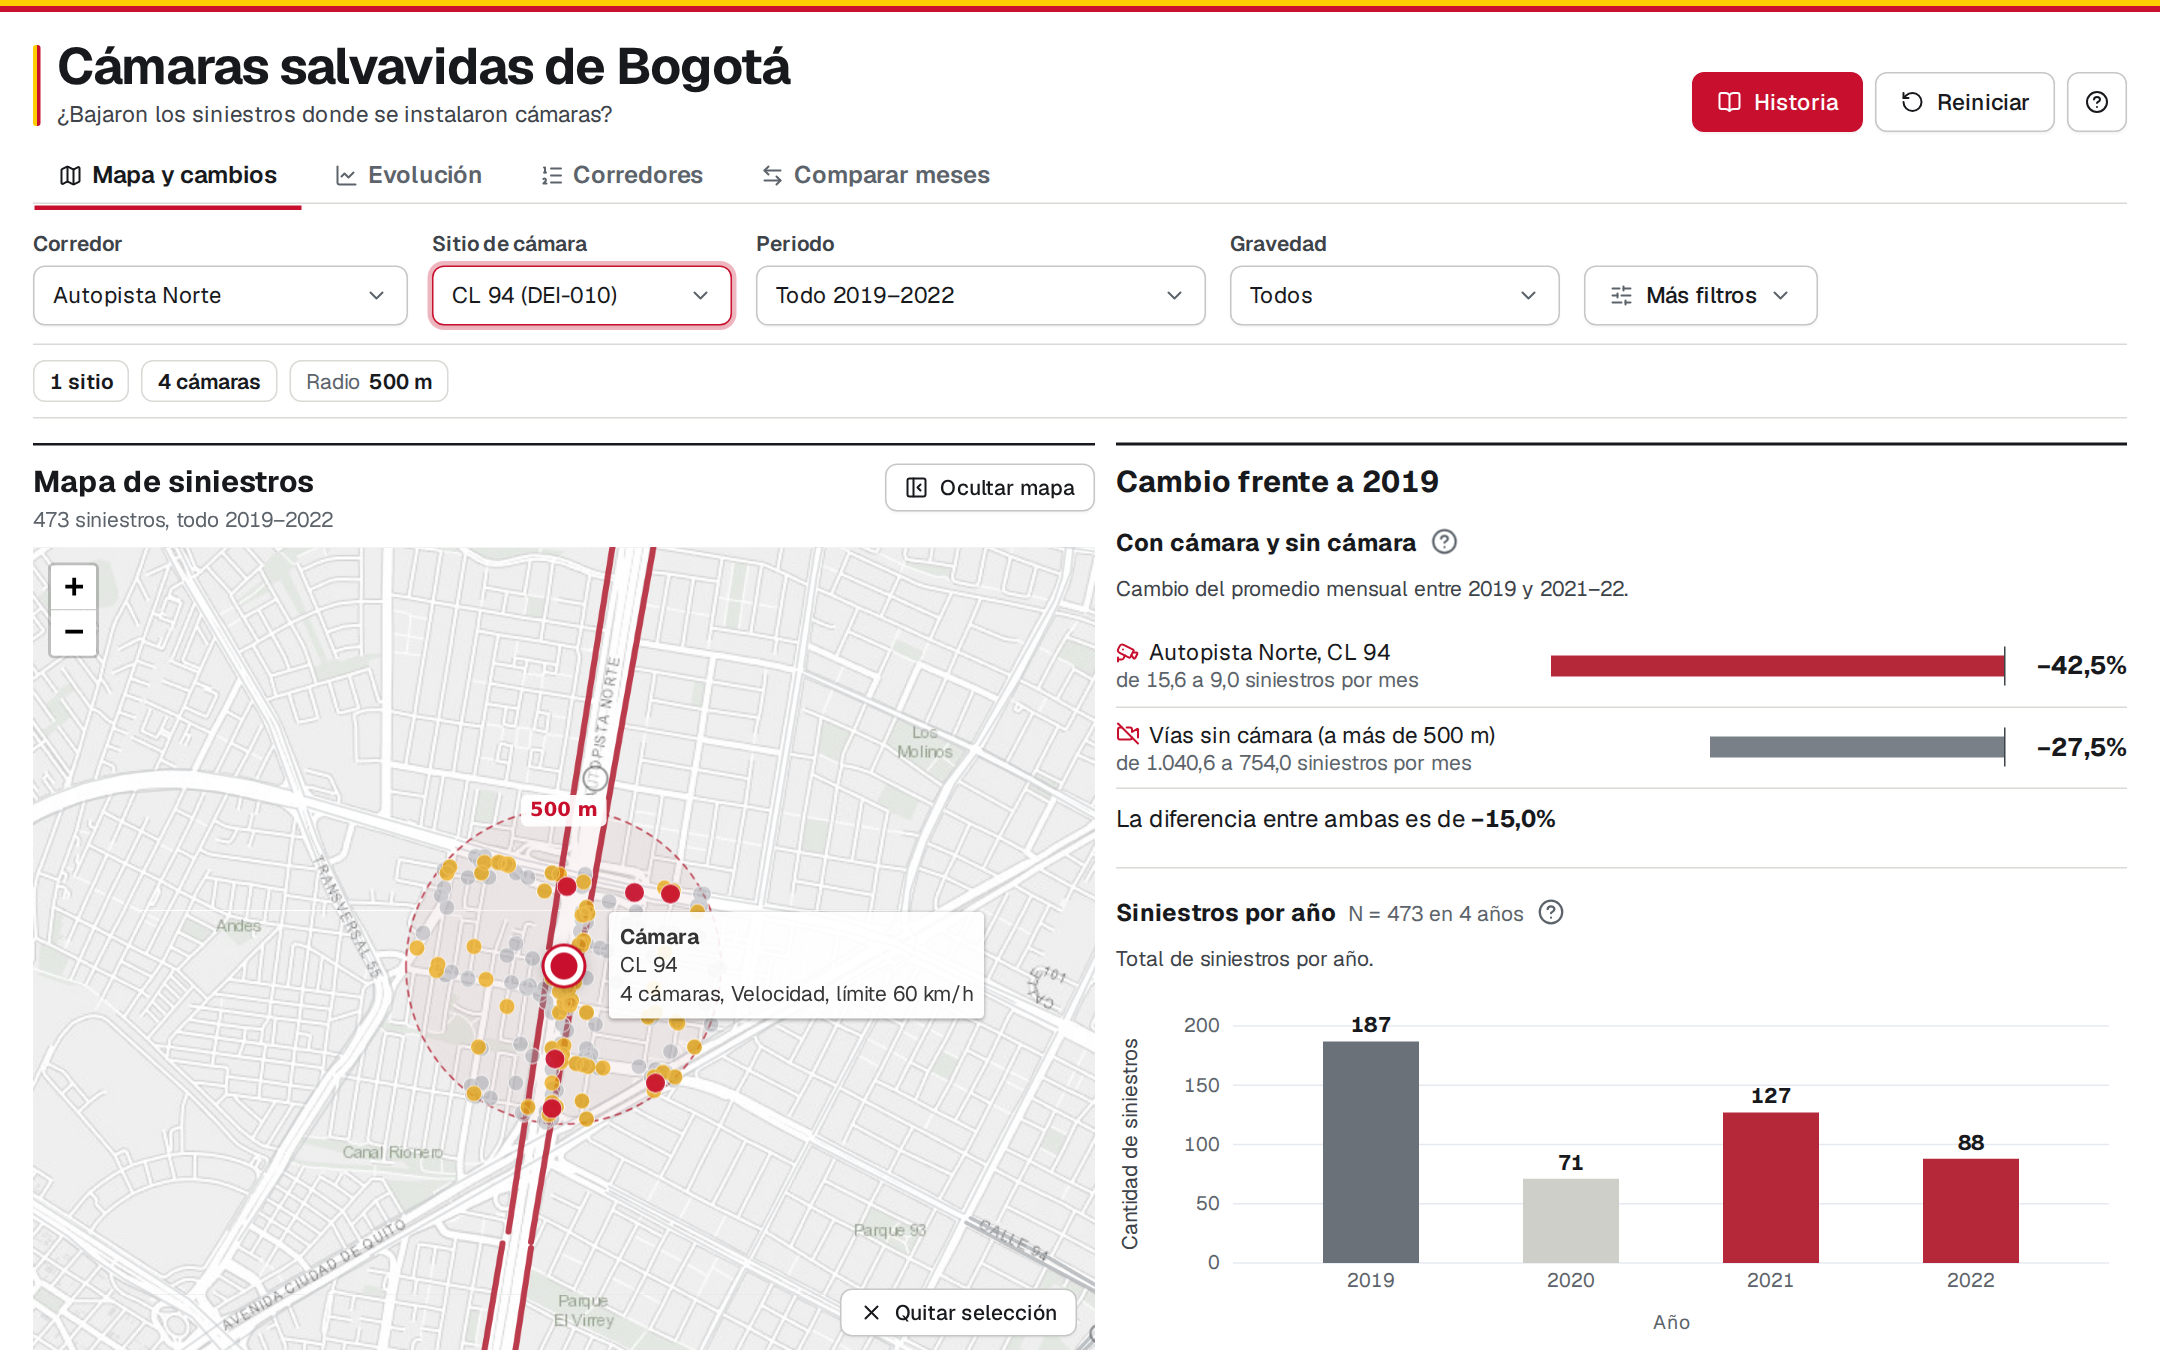
\includegraphics[width=0.49\linewidth,height=0.3\textheight,keepaspectratio]{f_sitio}\hfill
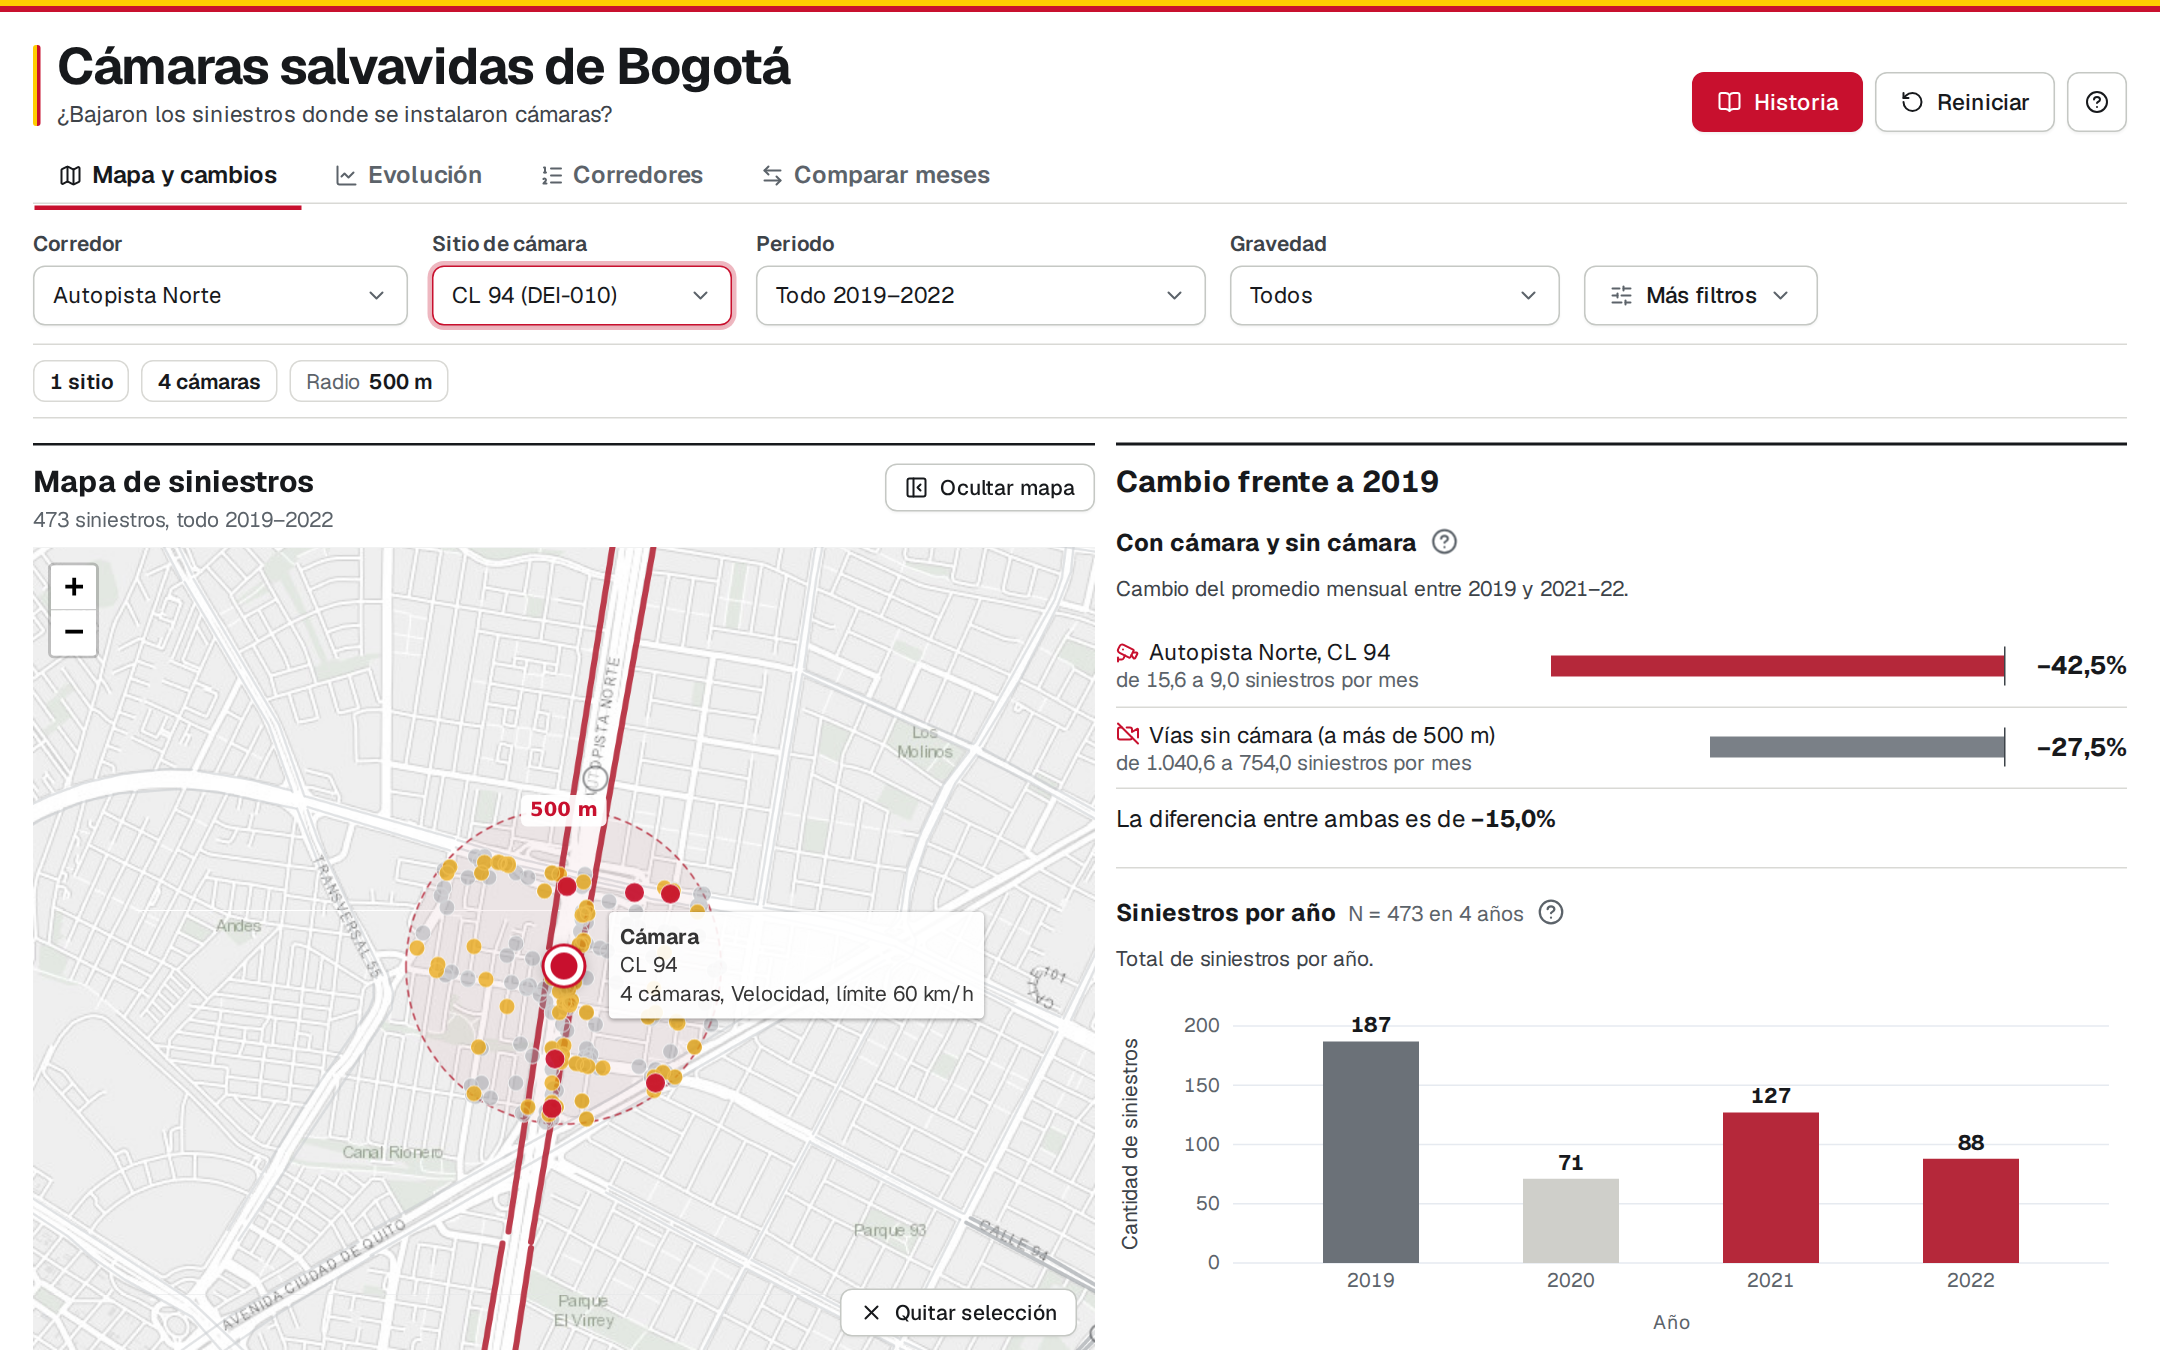
\includegraphics[width=0.49\linewidth,height=0.3\textheight,keepaspectratio]{f_corredor}
\caption{Un sitio seleccionado y los siniestros de todo el corredor}
\end{figure}

La información adicional se entrega cuando se pide, con tooltips que muestran solo datos y con un icono de ayuda junto a cada título que explica cómo leer la gráfica. Antes esas explicaciones estaban escritas a la vista y el dashboard parecía una guía, así que al moverlas quien ya sabe leer una gráfica no tiene que pasar por ellas y quien la ve por primera vez las encuentra al lado, también desde el celular con un toque.

\begin{figure}[H]\centering
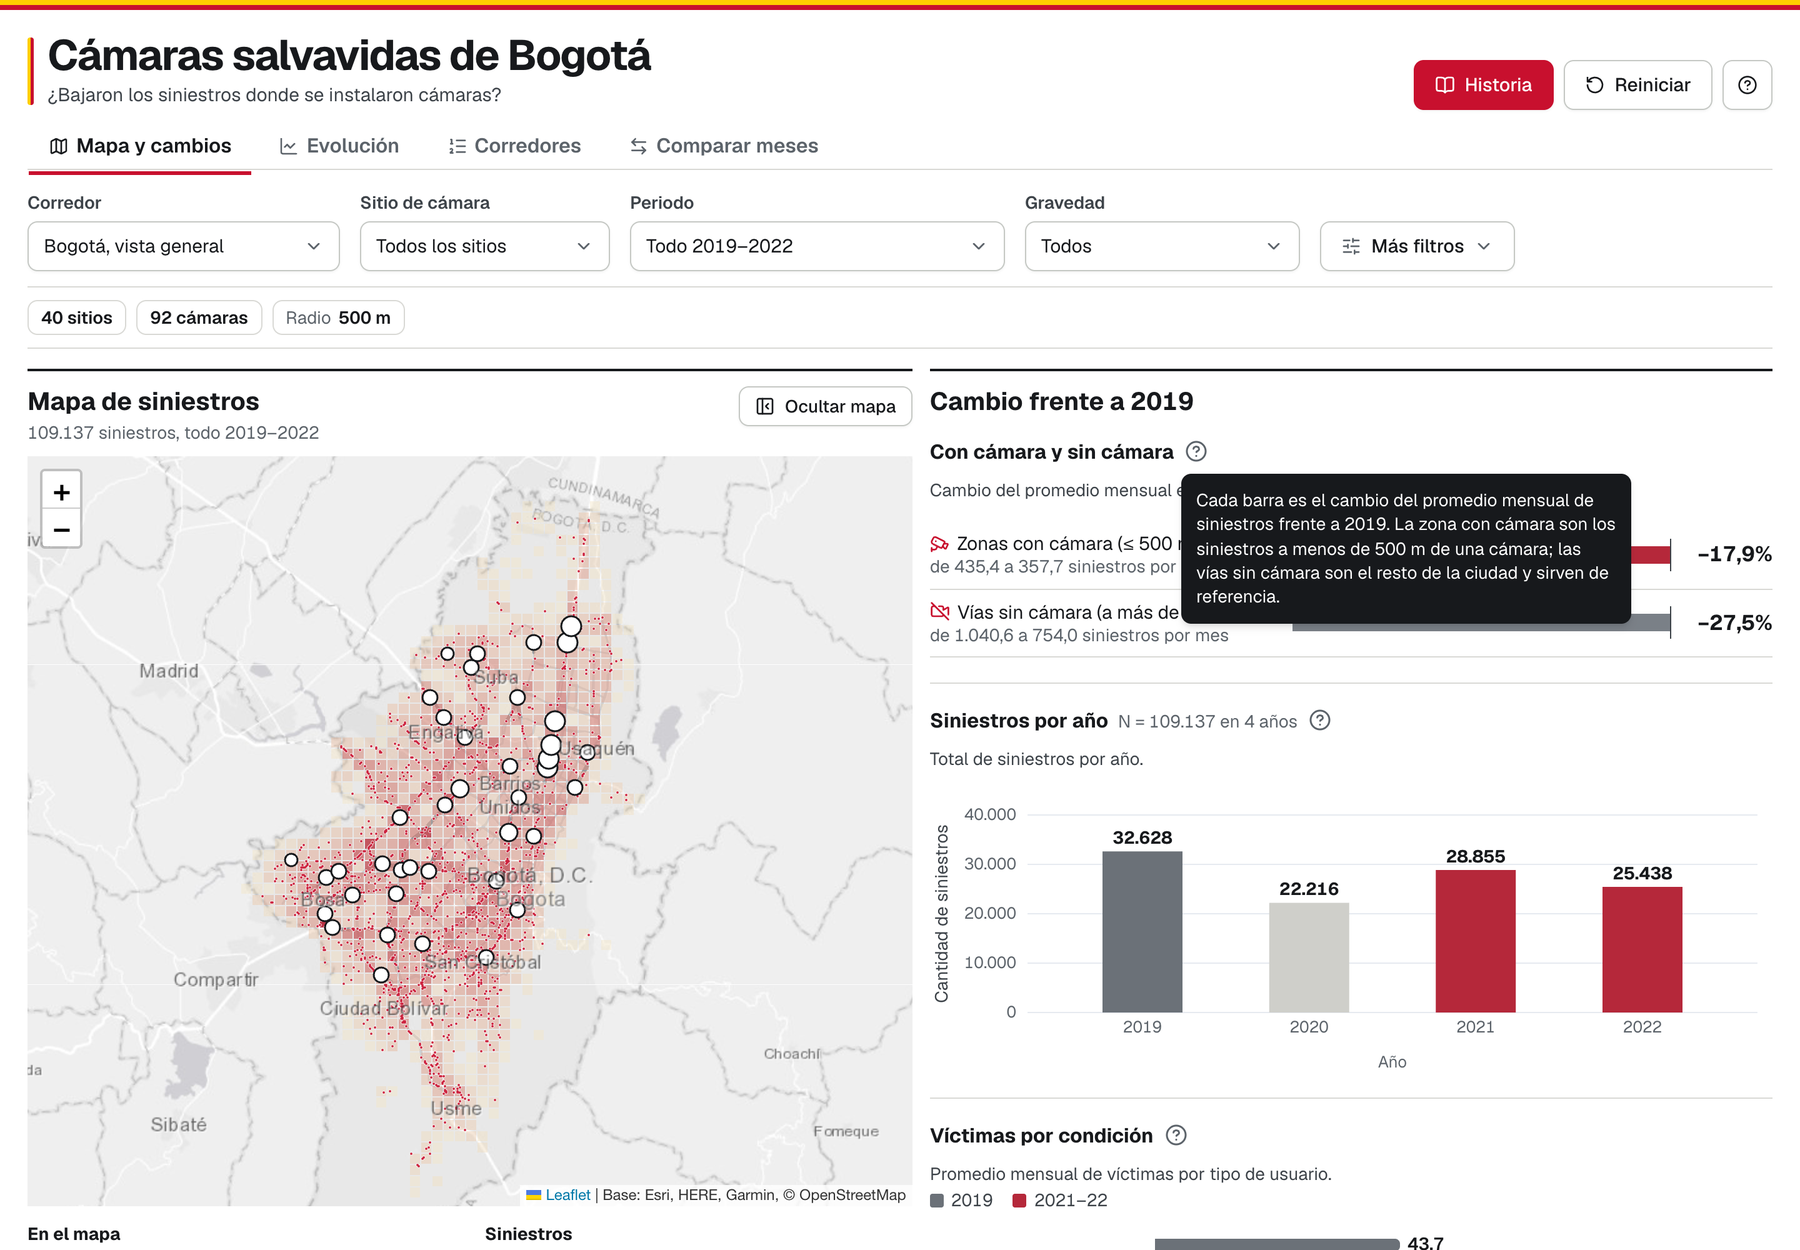
\includegraphics[width=0.7\linewidth,height=0.3\textheight,keepaspectratio]{f_ayuda}
\caption{Ayuda de lectura abierta sobre la gráfica}
\end{figure}

\subsection{Facetas, orientación y distintas pantallas}

Separamos el dashboard en cuatro vistas porque cada una responde un tipo de pregunta y juntas no cabían sin competir, de forma que Mapa y cambios da el panorama, Evolución se ocupa del cuándo, Corredores del cuál y Comparar meses deja armar una comparación propia. El orden de las pestañas va de lo general a lo particular y sus nombres dicen qué se va a encontrar, porque con nombres como ``Panorama'' o ``Serie'' no era claro. El mapa acompaña las vistas en las que el lugar aporta y queda siempre a la izquierda para no desorientar.

Todo sigue el principio ``overview first, zoom and filter, then details on demand'', ya que cada vista abre con todo el conjunto, el mapa y la serie permiten acercarse, los filtros reducen lo que se ve y los tooltips, las ayudas y la tarjeta de corredor agregan detalle cuando se pide. Así Diana puede quedarse en la primera lectura y Carolina llegar hasta el detalle sin que una le estorbe a la otra.

\begin{figure}[H]\centering
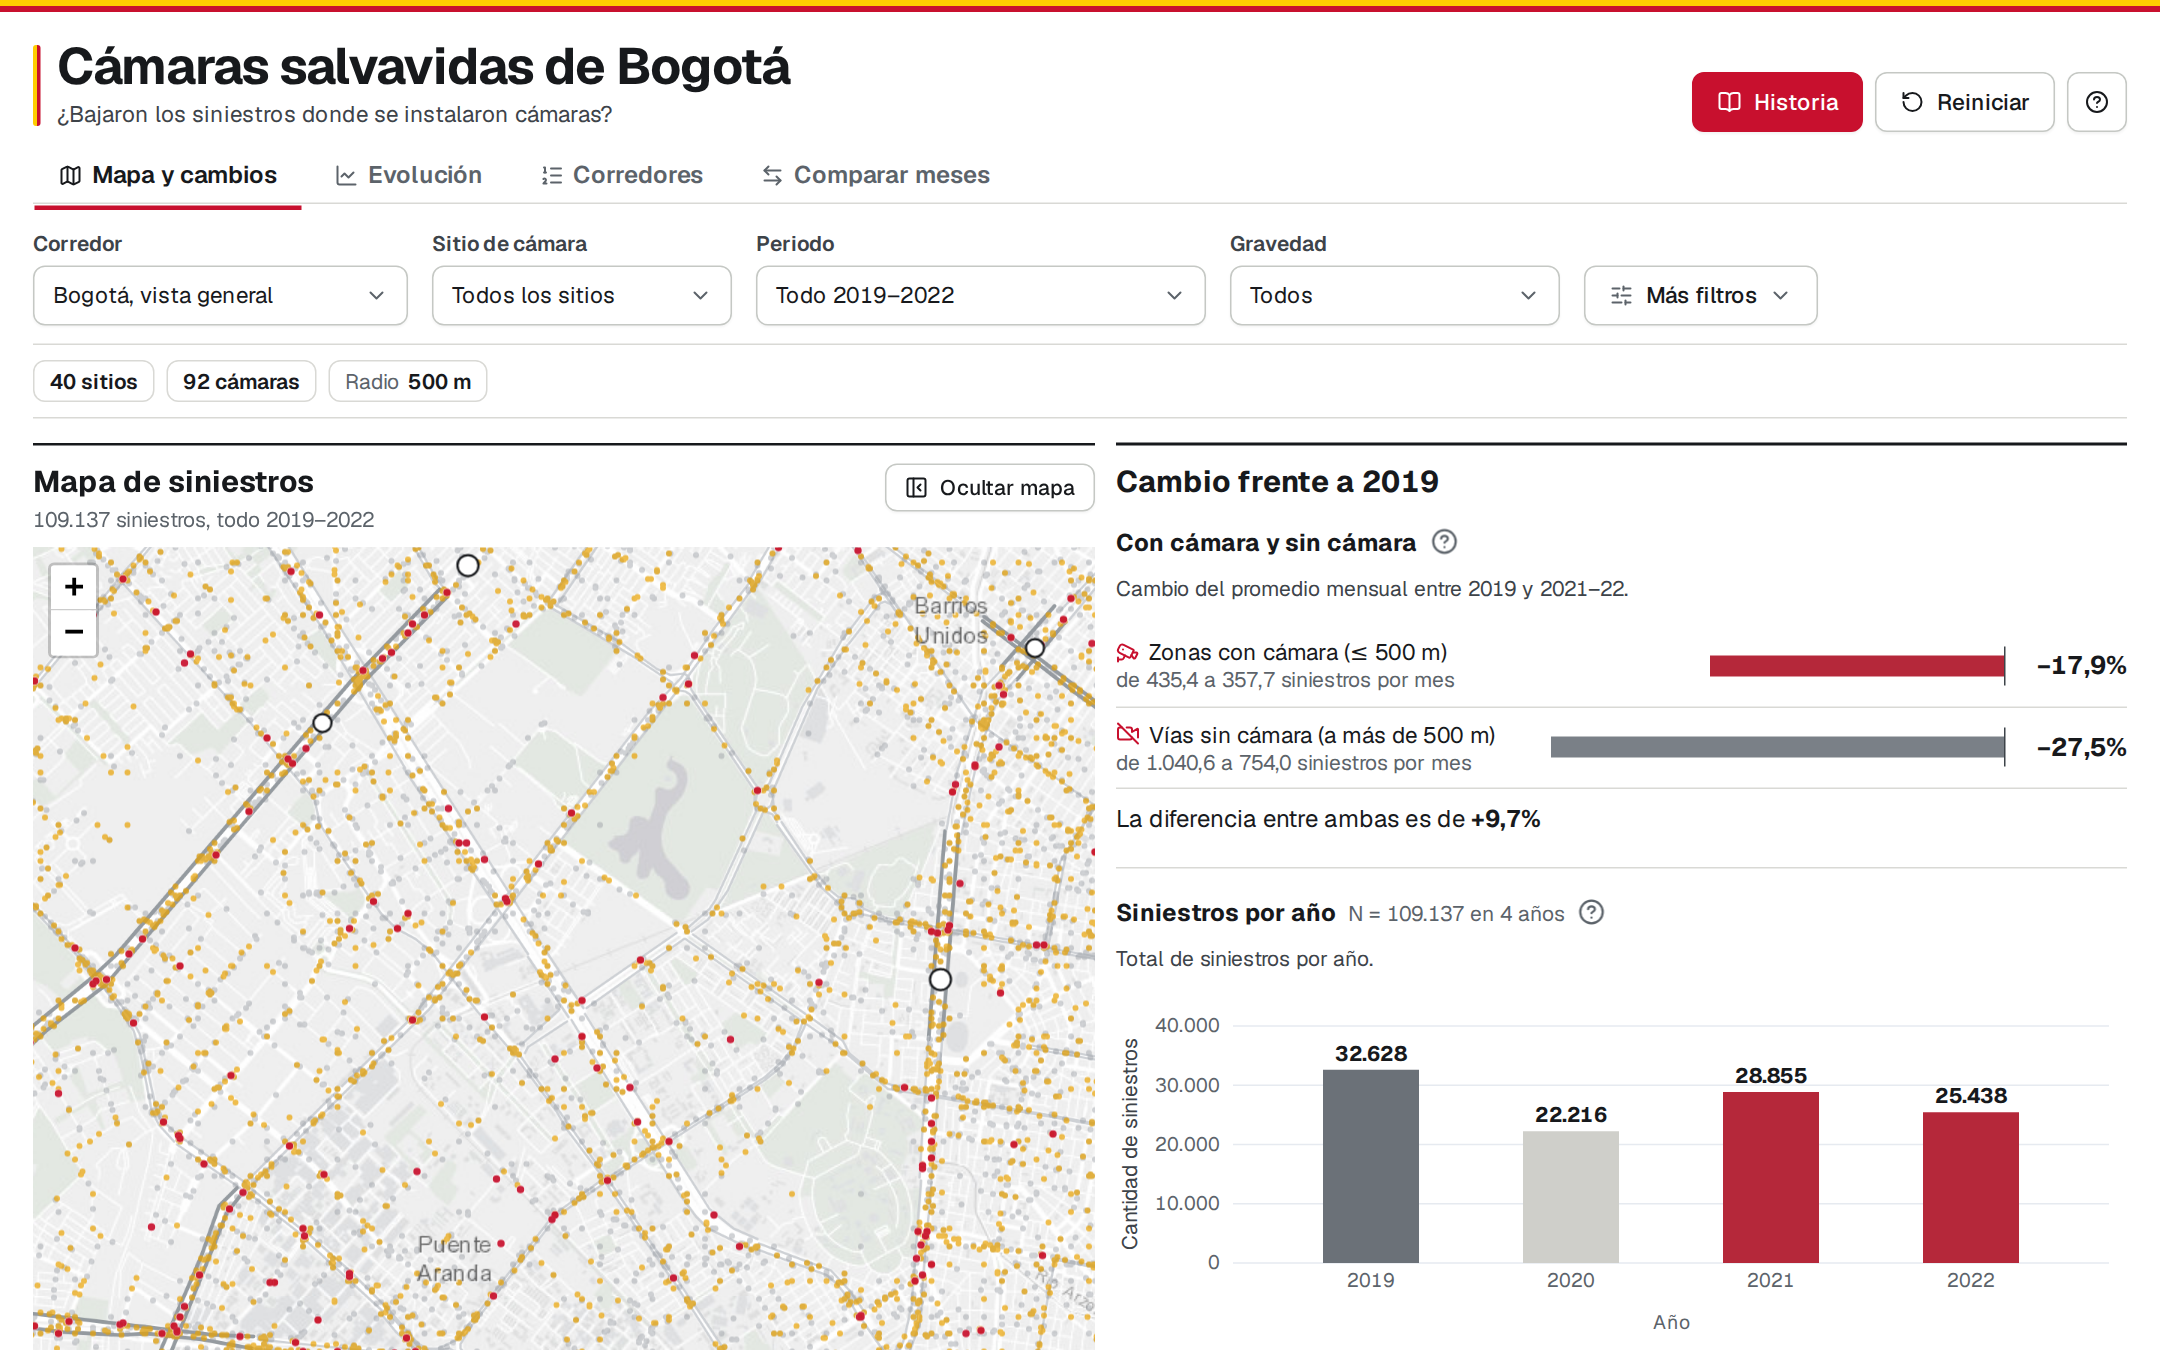
\includegraphics[width=0.49\linewidth,height=0.3\textheight,keepaspectratio]{ex_zoom}\hfill
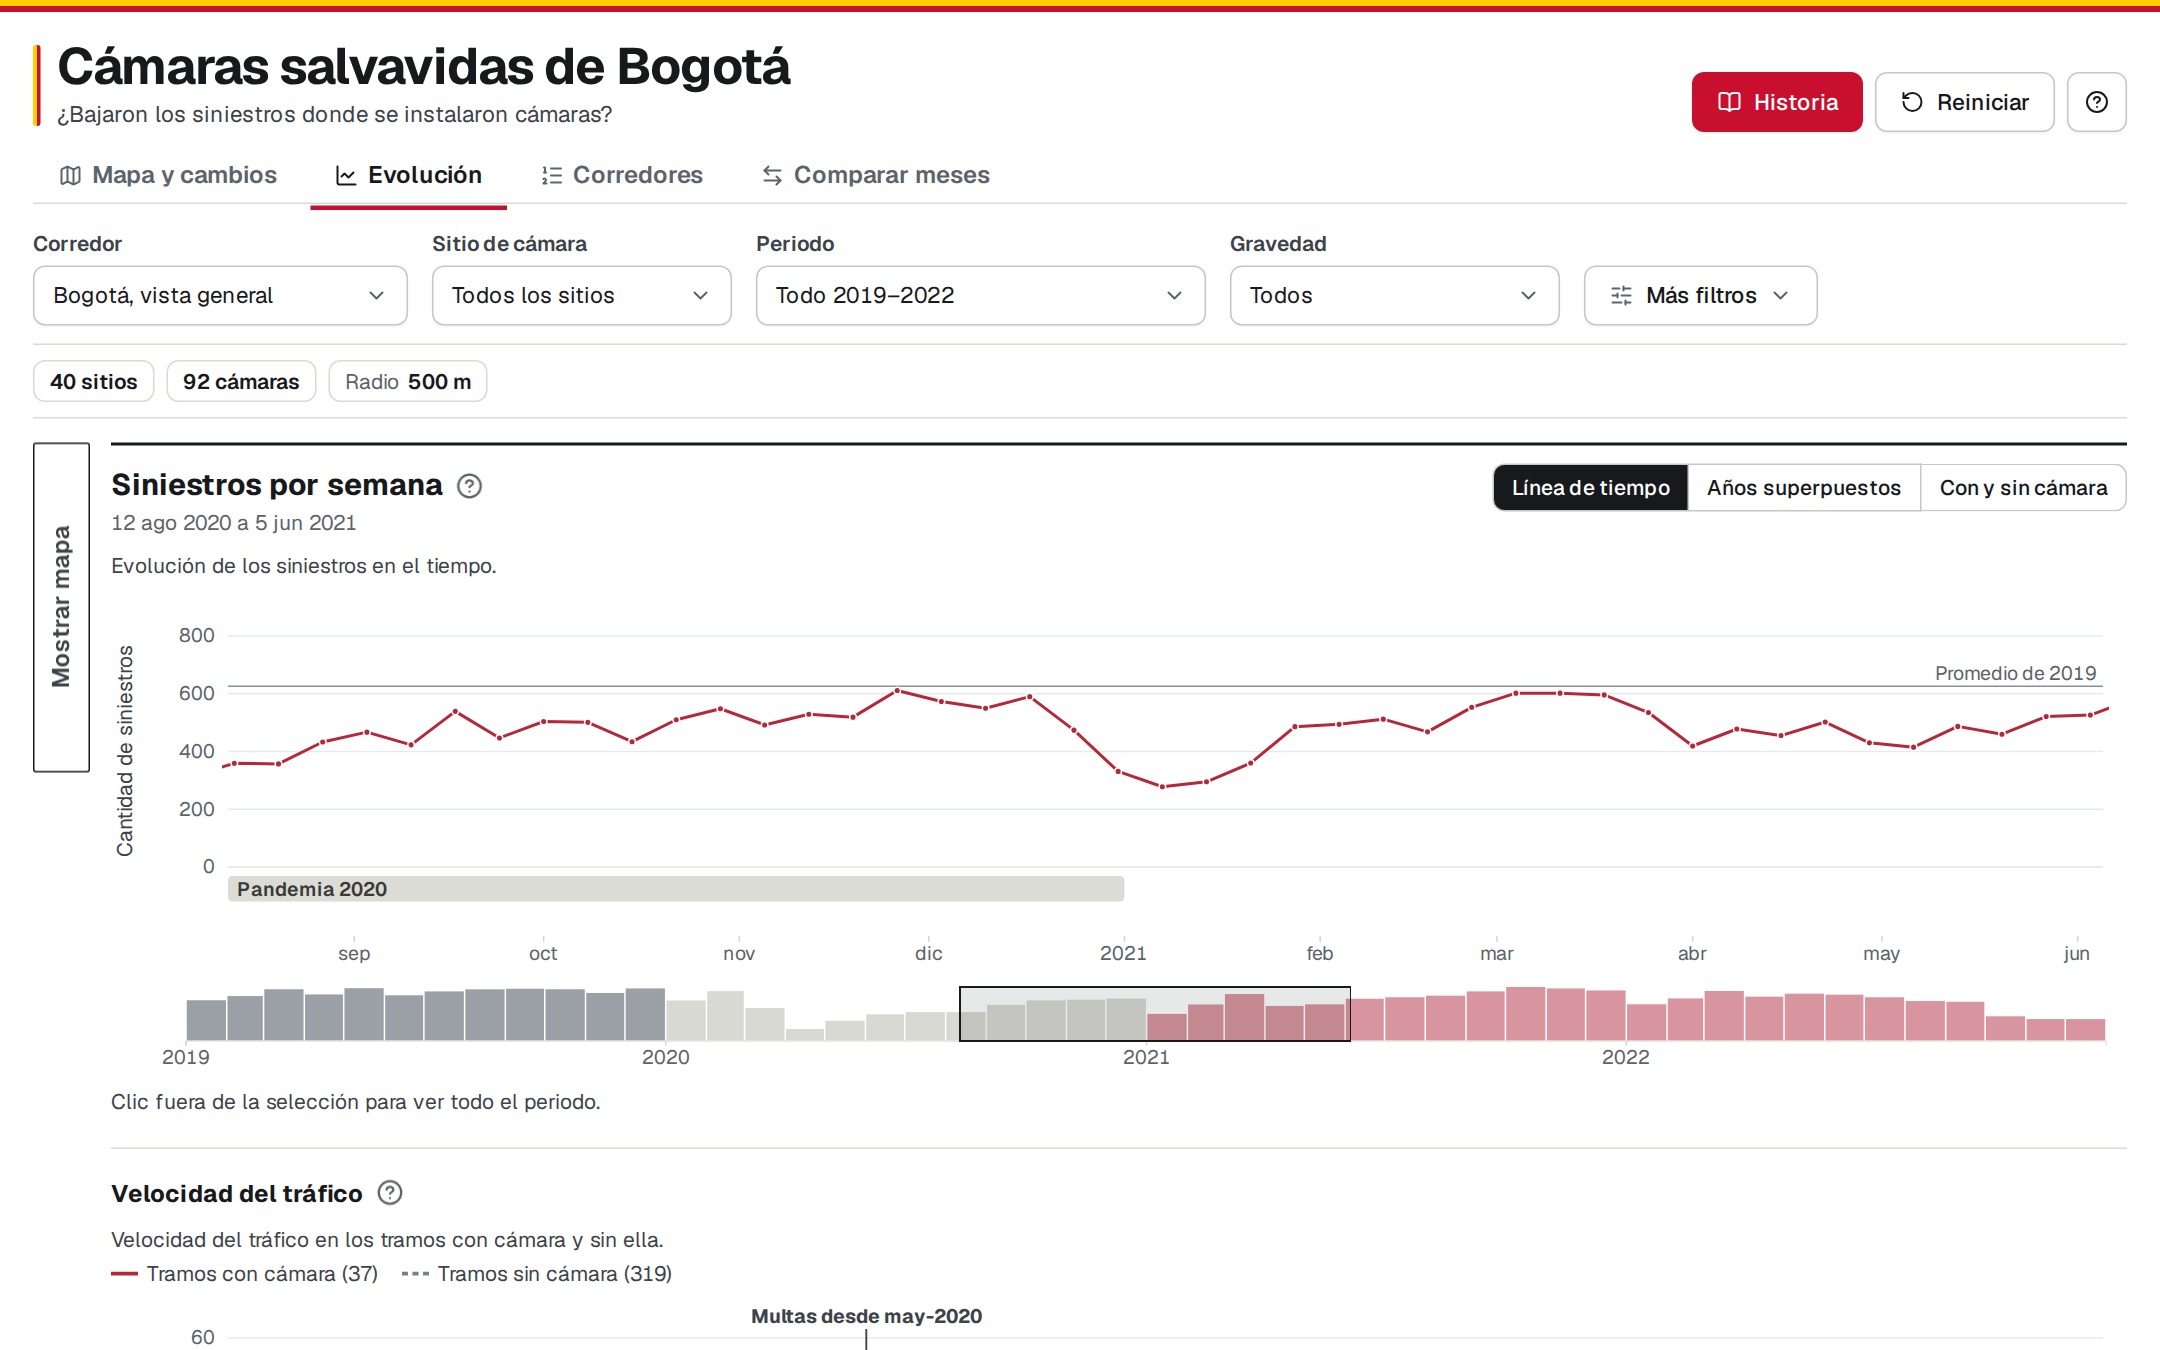
\includegraphics[width=0.49\linewidth,height=0.3\textheight,keepaspectratio]{ex_semanas}
\caption{Zoom en el mapa y en la serie}
\end{figure}

Para quien llega por primera vez hay una pantalla de inicio con la historia, un recorrido sobre cómo usar el dashboard, la exploración libre y las preguntas. Separamos el recorrido de la historia porque uno enseña a usar los controles señalándolos uno por uno y la otra cuenta qué se encontró. Además lo construimos como una aplicación web que calcula todo en el navegador, porque Carolina no puede instalar programas en su red y Andrés no programa, y en pantallas angostas los paneles se apilan y los filtros pasan a un panel inferior, pensando en que Diana entra casi siempre desde el celular.

\begin{figure}[H]\centering
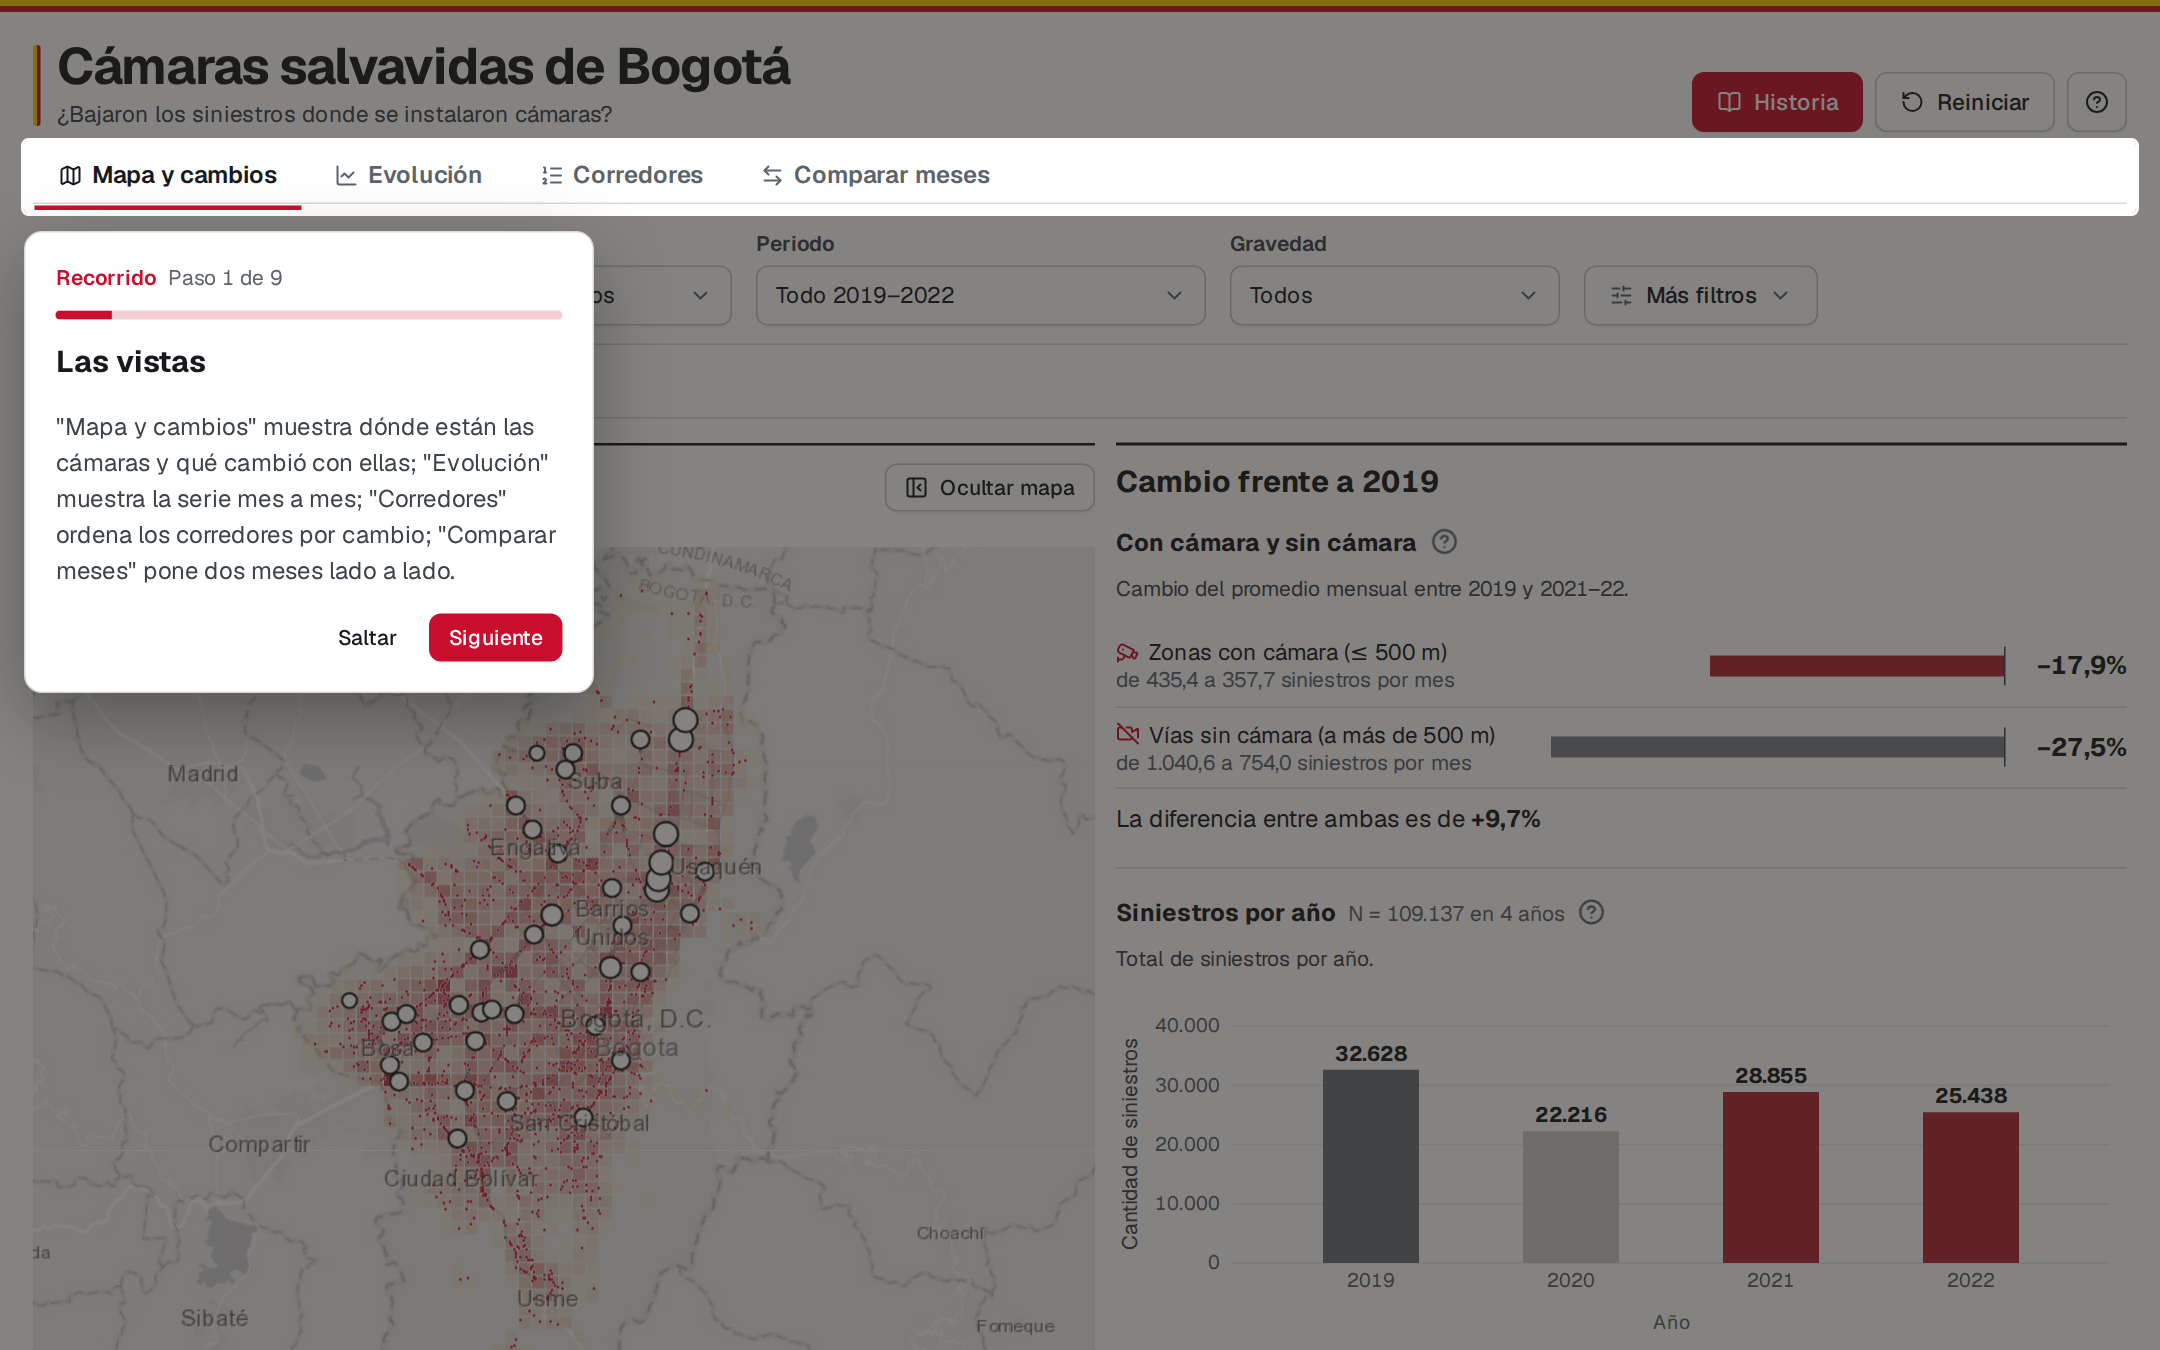
\includegraphics[height=0.28\textheight]{f_recorrido}\hfill
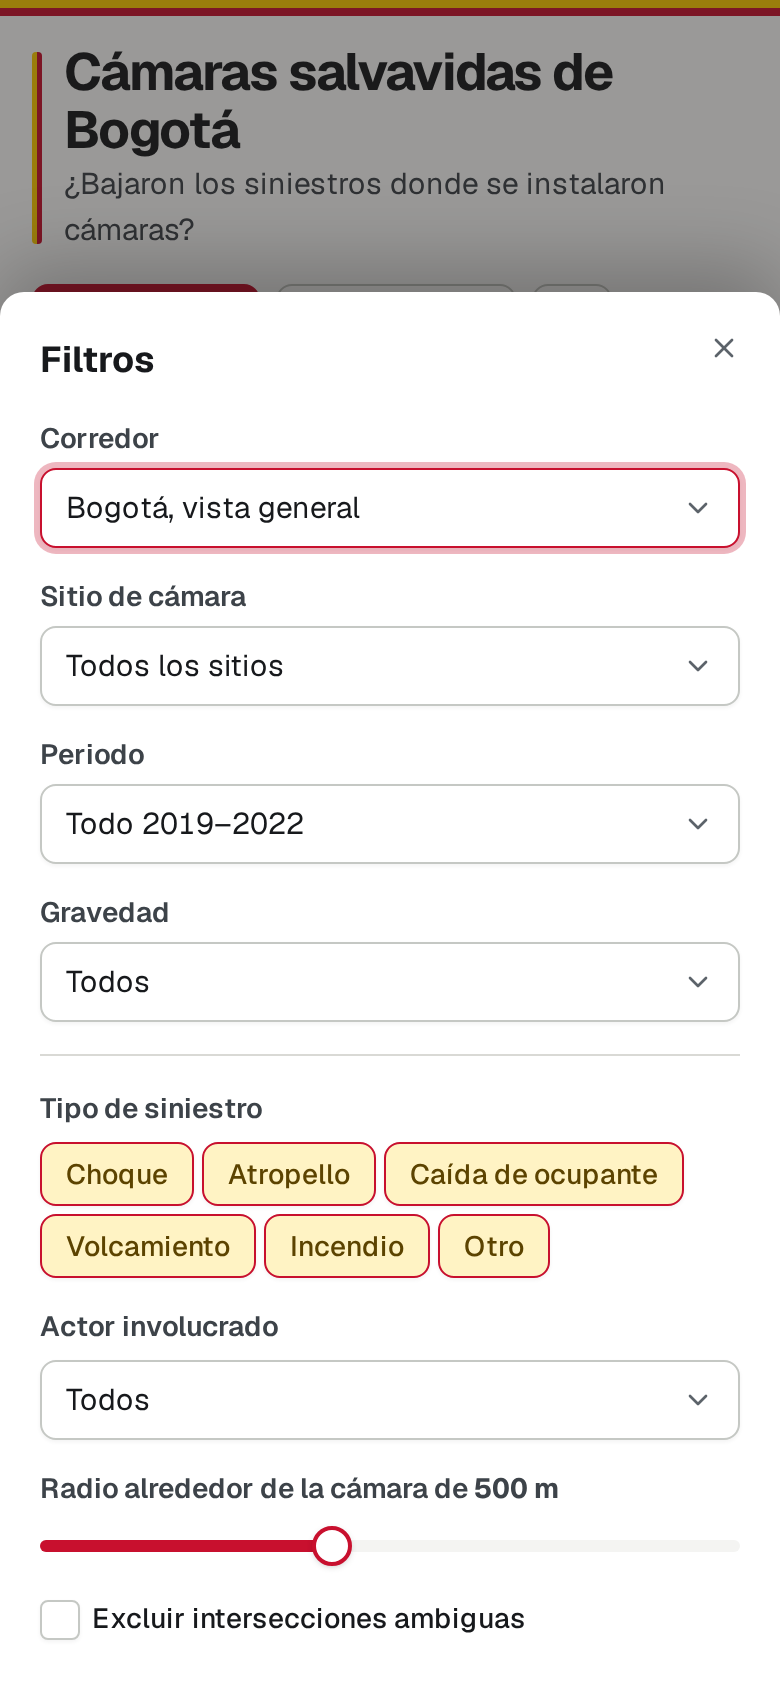
\includegraphics[height=0.28\textheight]{movil_filtros}
\caption{Recorrido guiado y filtros en el celular}
\end{figure}
\FloatBarrier
\section{Wireframes}


Nuestros primeros wireframes fueron interactivos y de baja fidelidad visual, con aspecto de boceto, pero usaban la red vial de Bogotá y conteos reales y se podían recorrer. Todas las pantallas compartían una retícula, con el mapa a la izquierda y el panel a la derecha, y se organizaban en diez pasos ligados a las tareas, con un modo de exploración libre y la opción de imprimirlos.

\figura[0.8]{w_ficha}{Wireframe de la ficha de la Av. Boyacá}
\begin{figure}[H]\centering
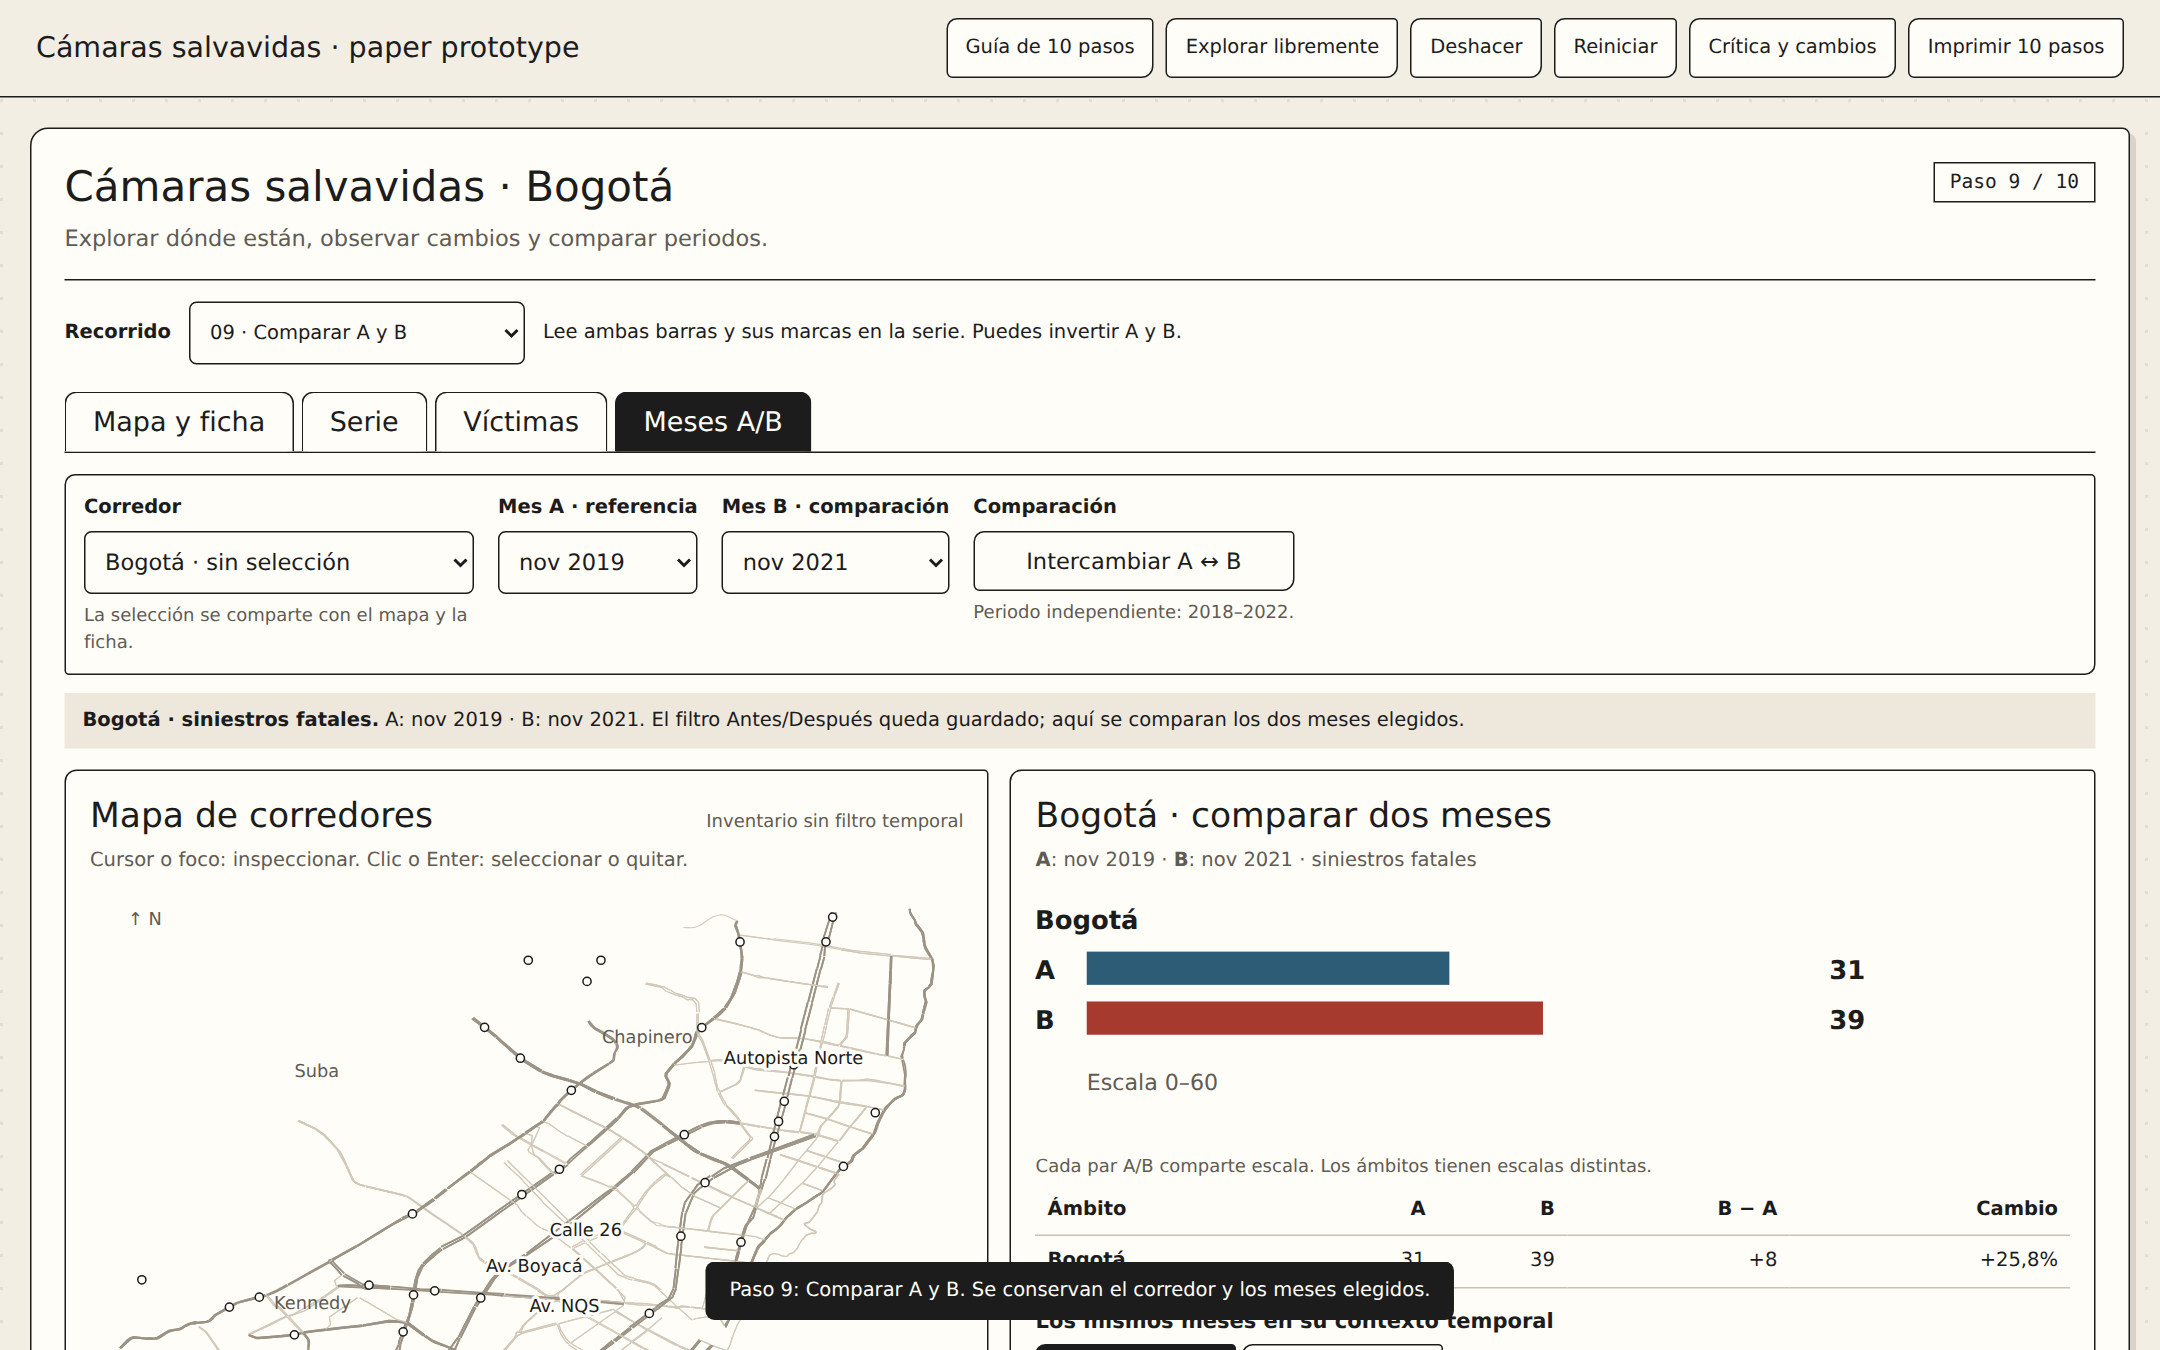
\includegraphics[width=0.49\linewidth]{w_comp}\hfill
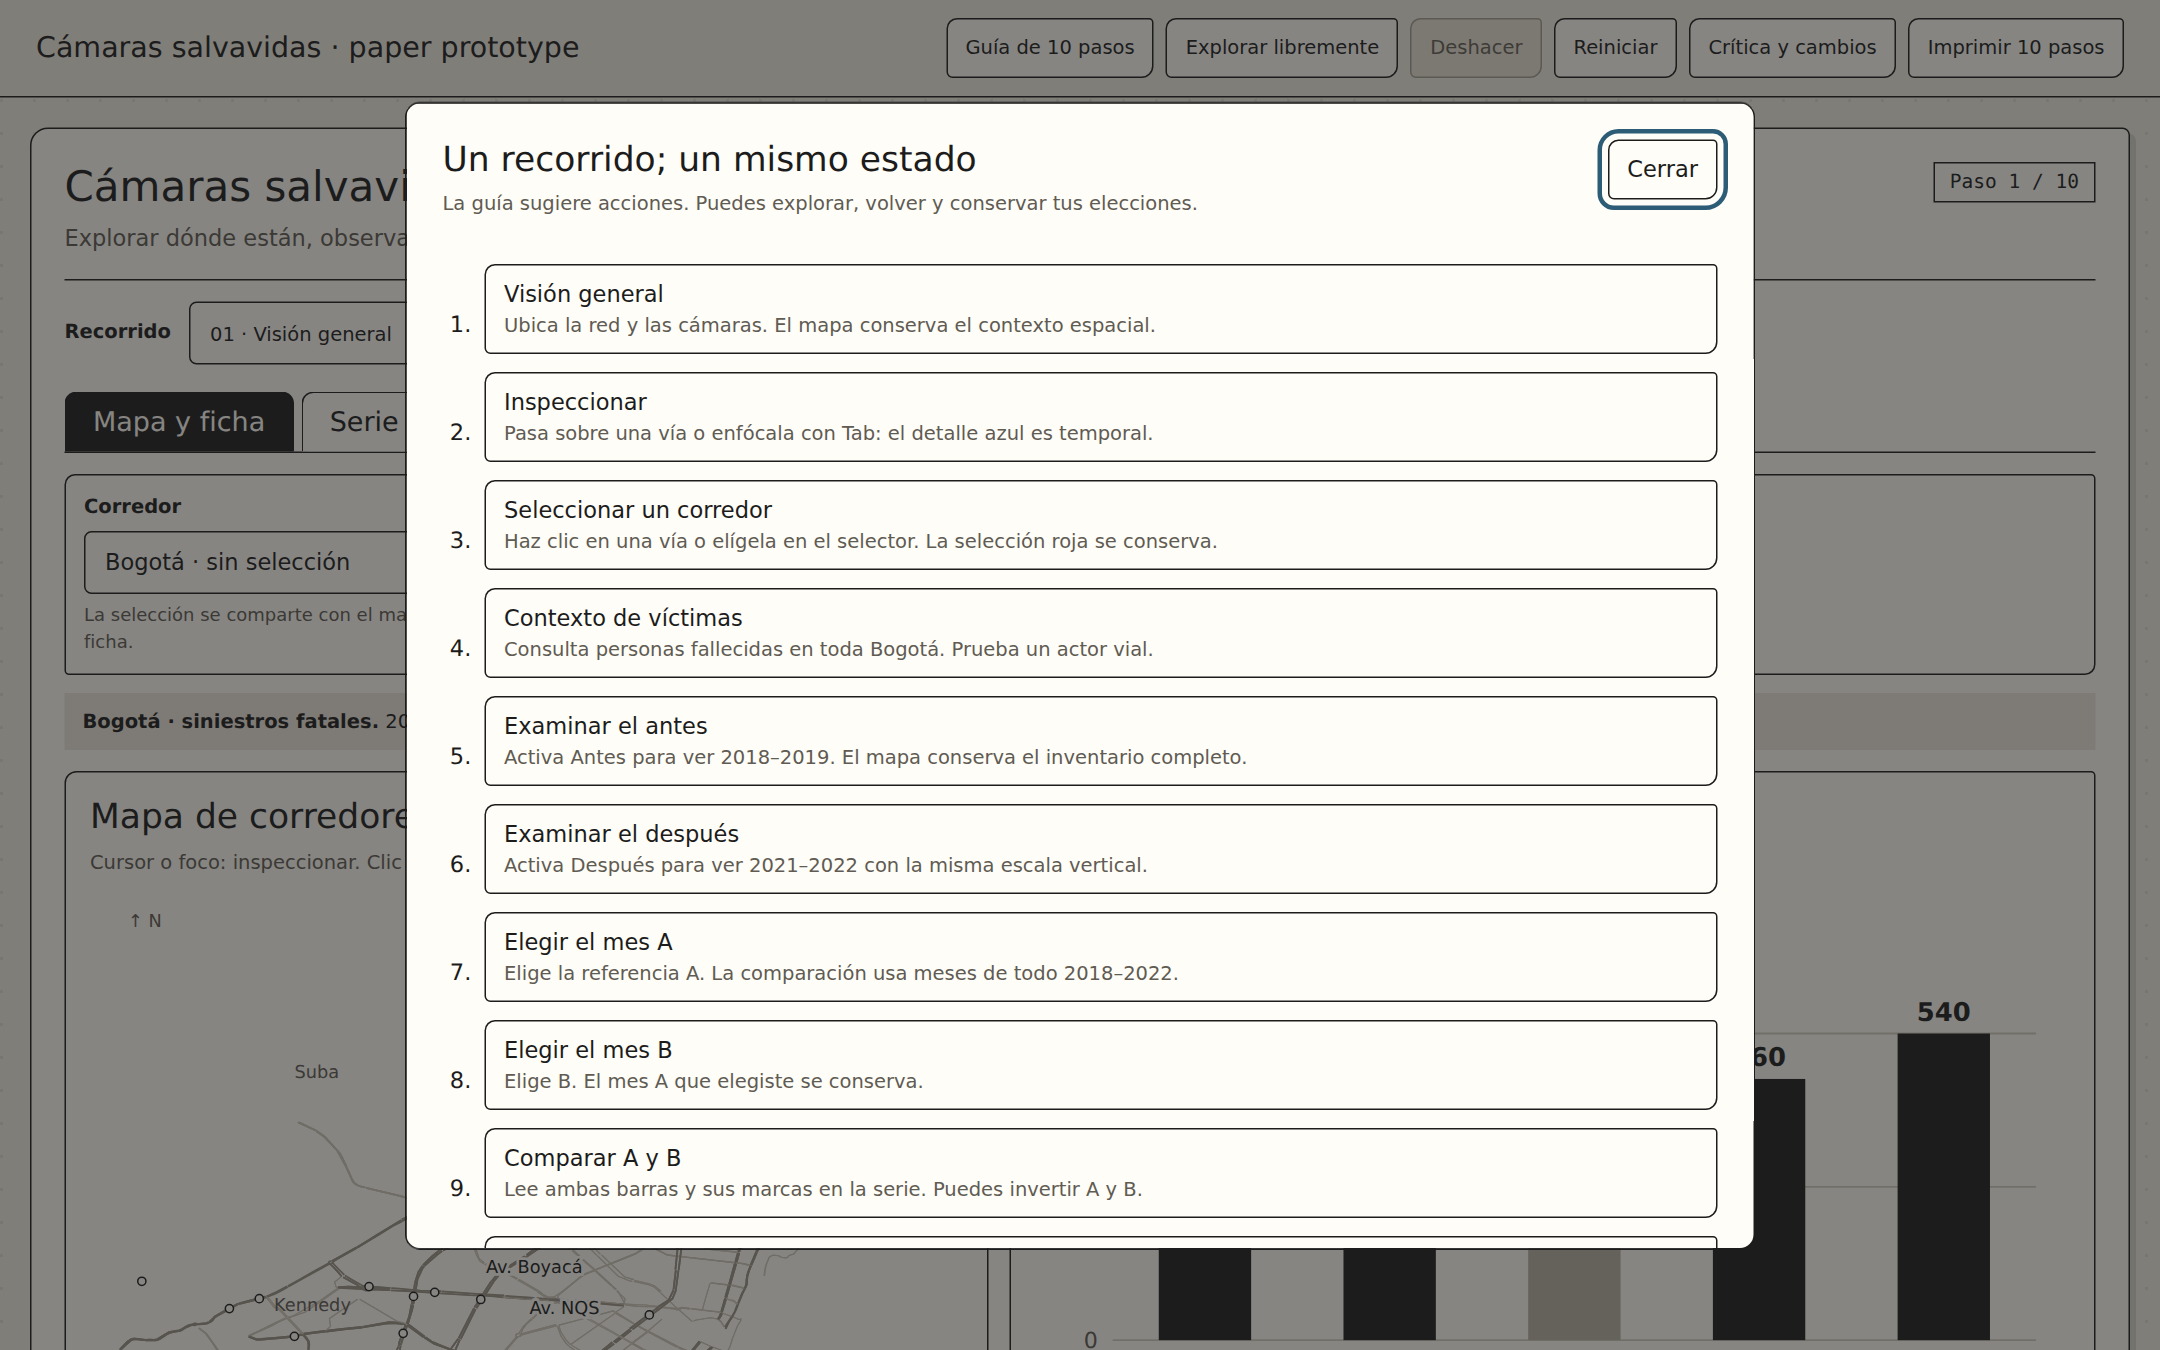
\includegraphics[width=0.49\linewidth]{w_guia}
\caption{Comparación de dos meses y pantalla de guía}
\end{figure}

En esta etapa revisamos la interacción con los criterios de Munzner, y de allí salieron reglas que mantenemos, como que seleccionar debe dejar un estado que se conserva, que un filtro debe cambiar lo que se muestra y que las dos cosas que se comparan deben verse al mismo tiempo. Antes de esa revisión varias transiciones de los wireframes no respetaban lo que el usuario había hecho en el paso anterior, por ejemplo al devolver un mes elegido a su valor inicial, y confundían la navegación de la guía con la manipulación de los datos. Separar ambas cosas fue lo que permitió después tener una historia guiada y una exploración libre sobre el mismo dashboard.

\begin{table}[H]\centering\small
\begin{tabularx}{\linewidth}{LL}
\toprule
\textbf{Wireframes} & \textbf{Dashboard actual}\\
\midrule
Mapa junto a un panel de análisis & Se conserva.\\
Recorrido guiado y exploración libre & Se conserva como copa de martini.\\
Un solo corredor con datos mensuales, la Av. Boyacá & Los 18 corredores.\\
Solo siniestros con muertos & Cuatro niveles de gravedad.\\
``Antes'' como 2018 y 2019 & ``Antes'' es solo 2019.\\
Un mes A y un mes B & Grupos de meses.\\
Cifras escritas a mano & Cifras calculadas con los datos.\\
\bottomrule
\end{tabularx}
\caption{Qué conservamos y qué cambiamos}
\end{table}

\pendiente{Agregar otros wireframes del equipo, si los hay.}

\clearpage
\section{Mockups}

El mockup con el que probamos la interacción fue un paper prototype, y lo pensamos como una versión en papel de lo que queríamos construir. Las piezas las movíamos nosotros, de modo que quien probaba decía o señalaba qué haría y respondíamos cambiando la pieza como lo haría después la aplicación. En esta sección lo ponemos al lado de la versión final para que se vea qué se mantuvo, qué cambió y por qué.

\subsection{El paper prototype frente al dashboard}

El prototipo está compuesto por seis hojas A4, en las que las dos primeras son bases de montaje, la tercera trae los controles para recortar, la cuarta y la quinta las piezas que cambian al seleccionar o filtrar y la sexta las tarjetas de los meses con sus resultados, junto con una guía que nos indicaba qué pieza poner en cada momento. Lo limitamos a un caso, la Av. Boyacá, con siniestros fatales de 2018 a 2022, porque en papel cada combinación de filtros es una pieza más y lo que queríamos probar era el recorrido de seleccionar, filtrar y comparar, no la cantidad de opciones.

En las siguientes fotos se ve la prueba en clase, con la base montada, las piezas de la selección de la Av. Boyacá superpuestas y alrededor las tiras de pestañas, periodos, meses y resultados que íbamos cambiando a medida que la persona avanzaba. Trabajar así nos permitió probar la secuencia completa sin haber programado nada y notar en el momento qué respuesta no teníamos prevista.

\begin{figure}[H]\centering
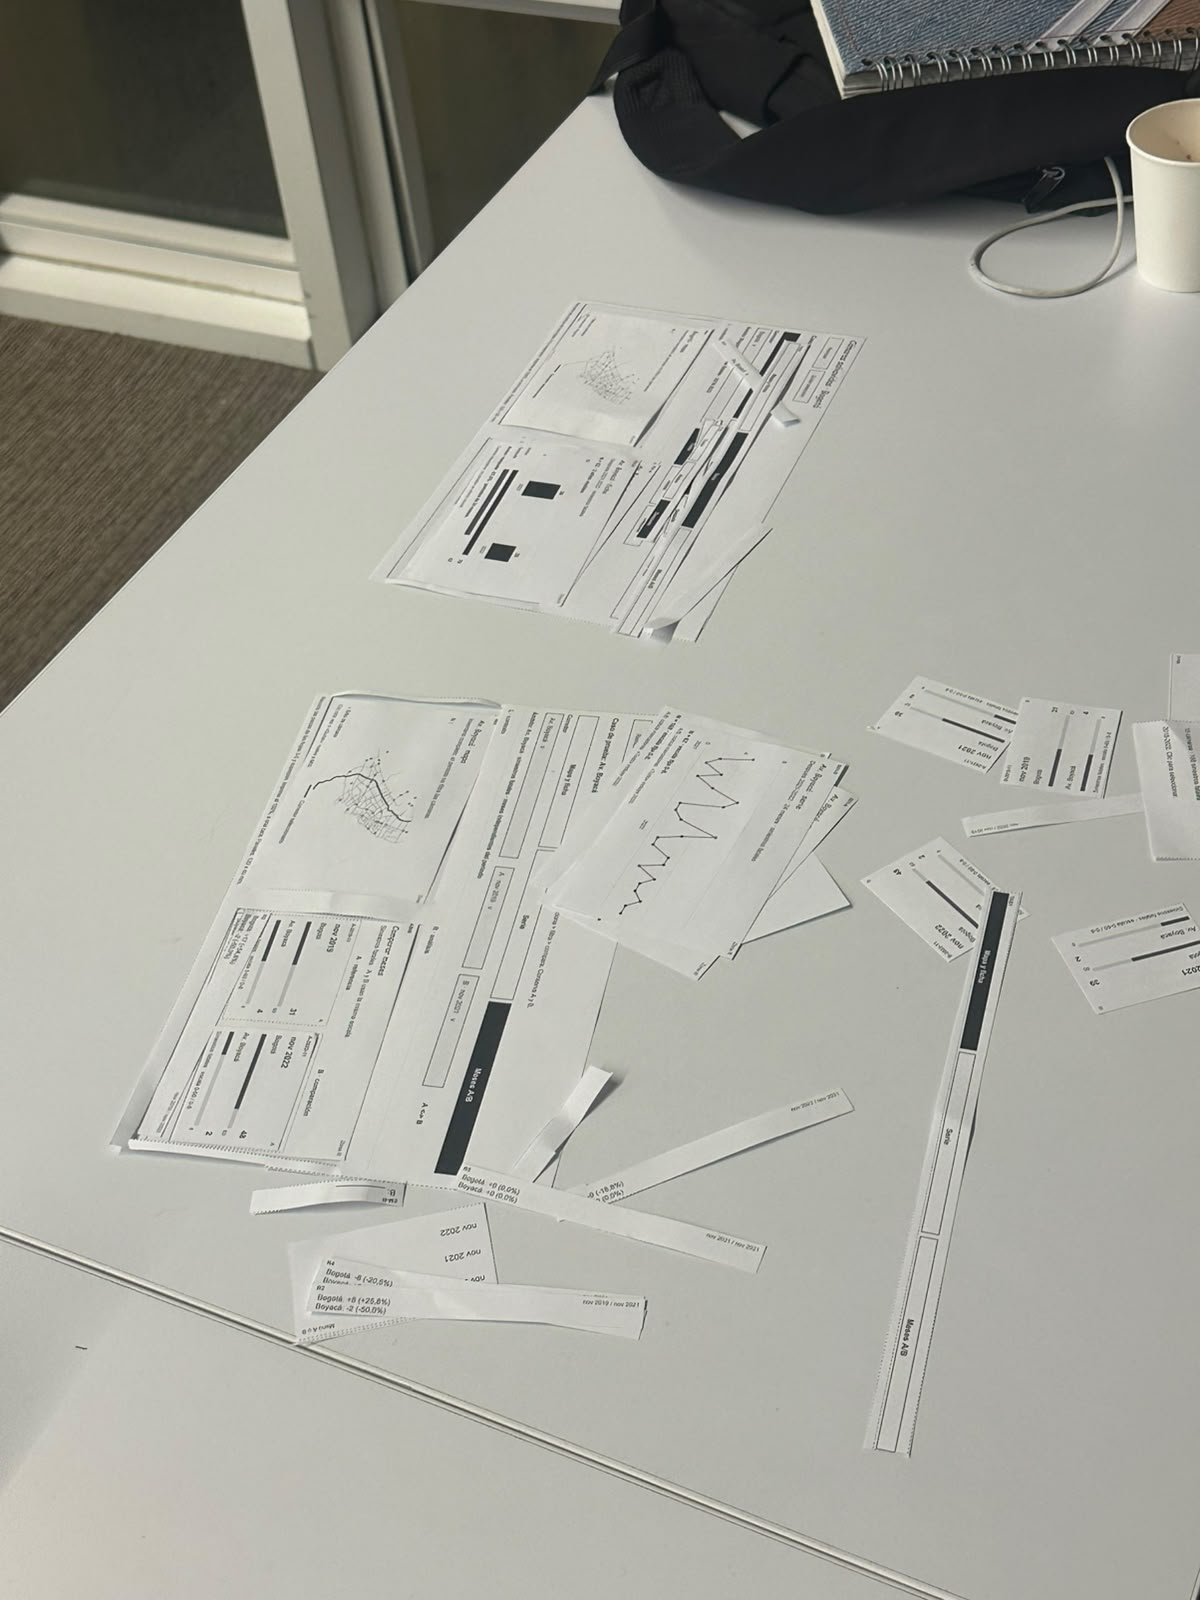
\includegraphics[height=7.6cm]{clase1}\hfill
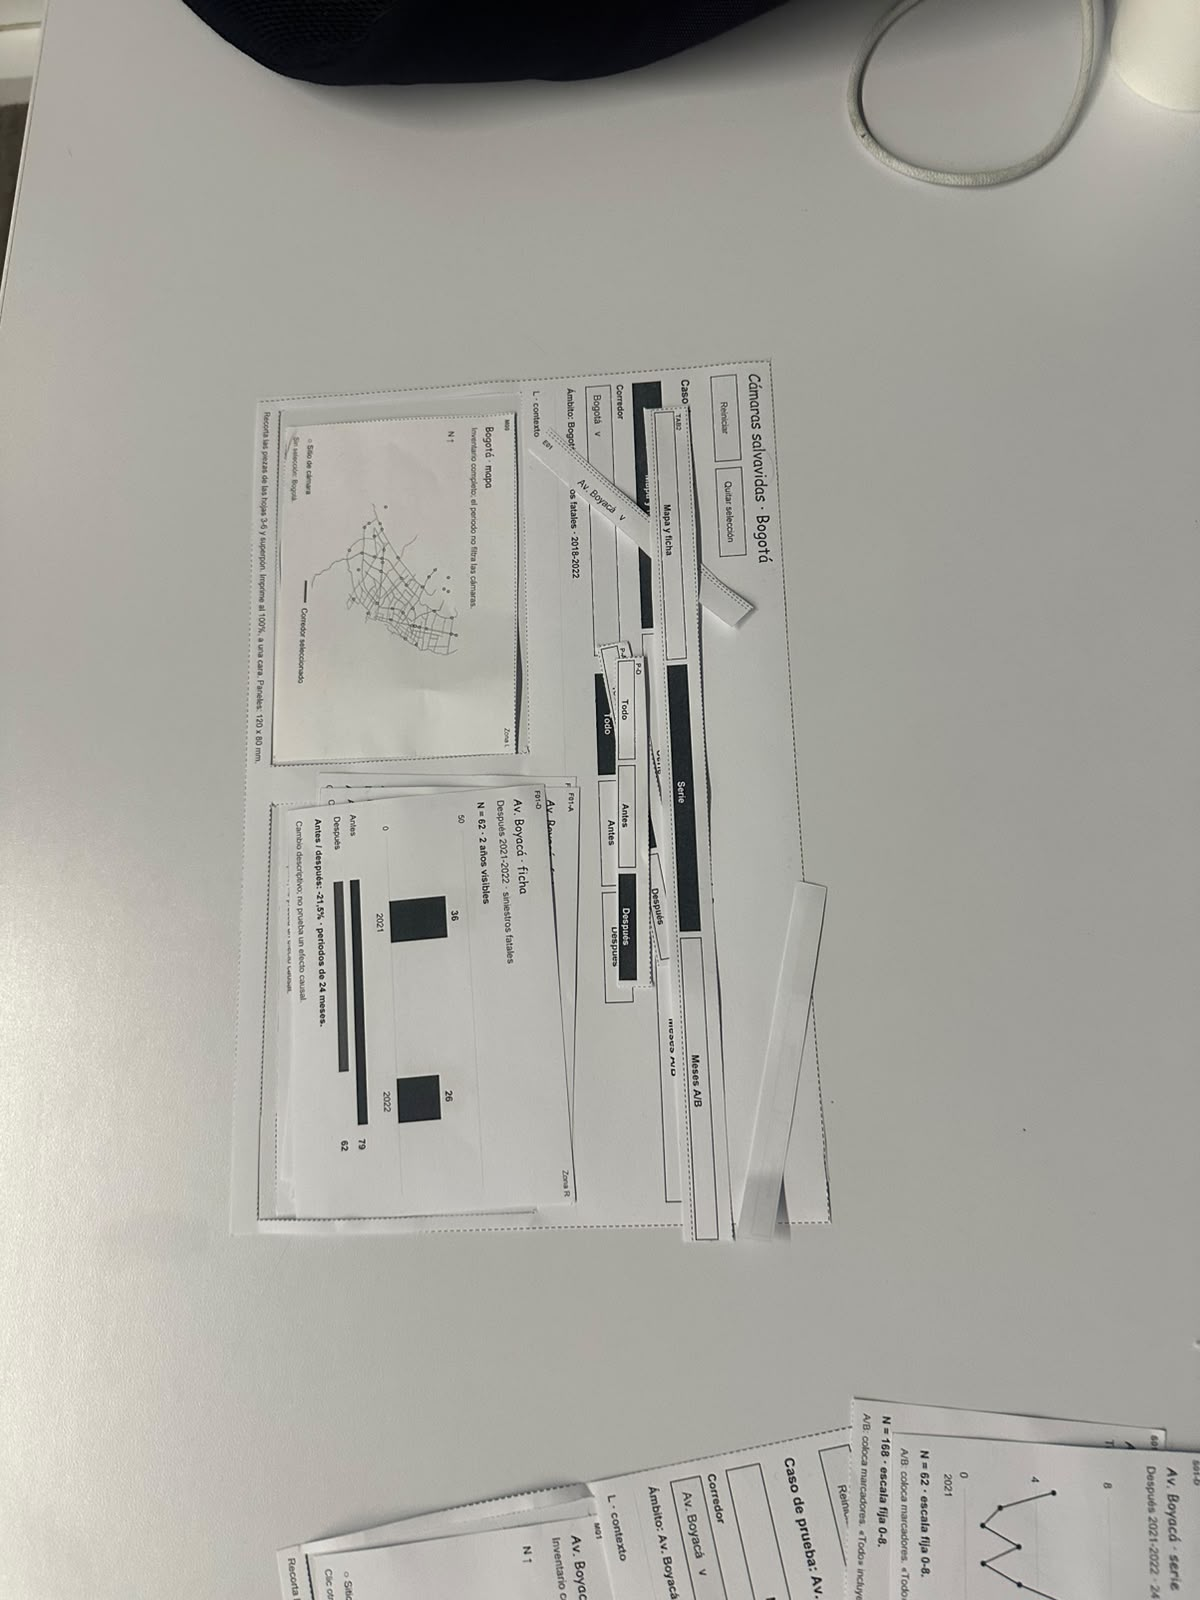
\includegraphics[angle=90,height=7.6cm]{clase2}
\caption{Prueba del paper prototype en clase}
\end{figure}

La primera base ya tenía la estructura que conservamos, con las vistas arriba, los filtros debajo, el mapa a la izquierda y el análisis a la derecha. La ficha mostraba los siniestros por año y dos barras de antes y después, y aquí está el cambio más importante, porque en papel no había ninguna referencia y solo se podía decir si la cifra había subido o bajado. En la versión final las barras muestran el cambio porcentual de la zona con cámara junto al de las vías sin cámara, así que la pregunta pasa de ``bajó o no'' a ``bajó más o menos que donde no hay cámara''. También crecieron los filtros, que pasaron de corredor y periodo a incluir sitio, gravedad y ``Más filtros'', como nos pidieron en los comentarios.

\begin{figure}[H]\centering
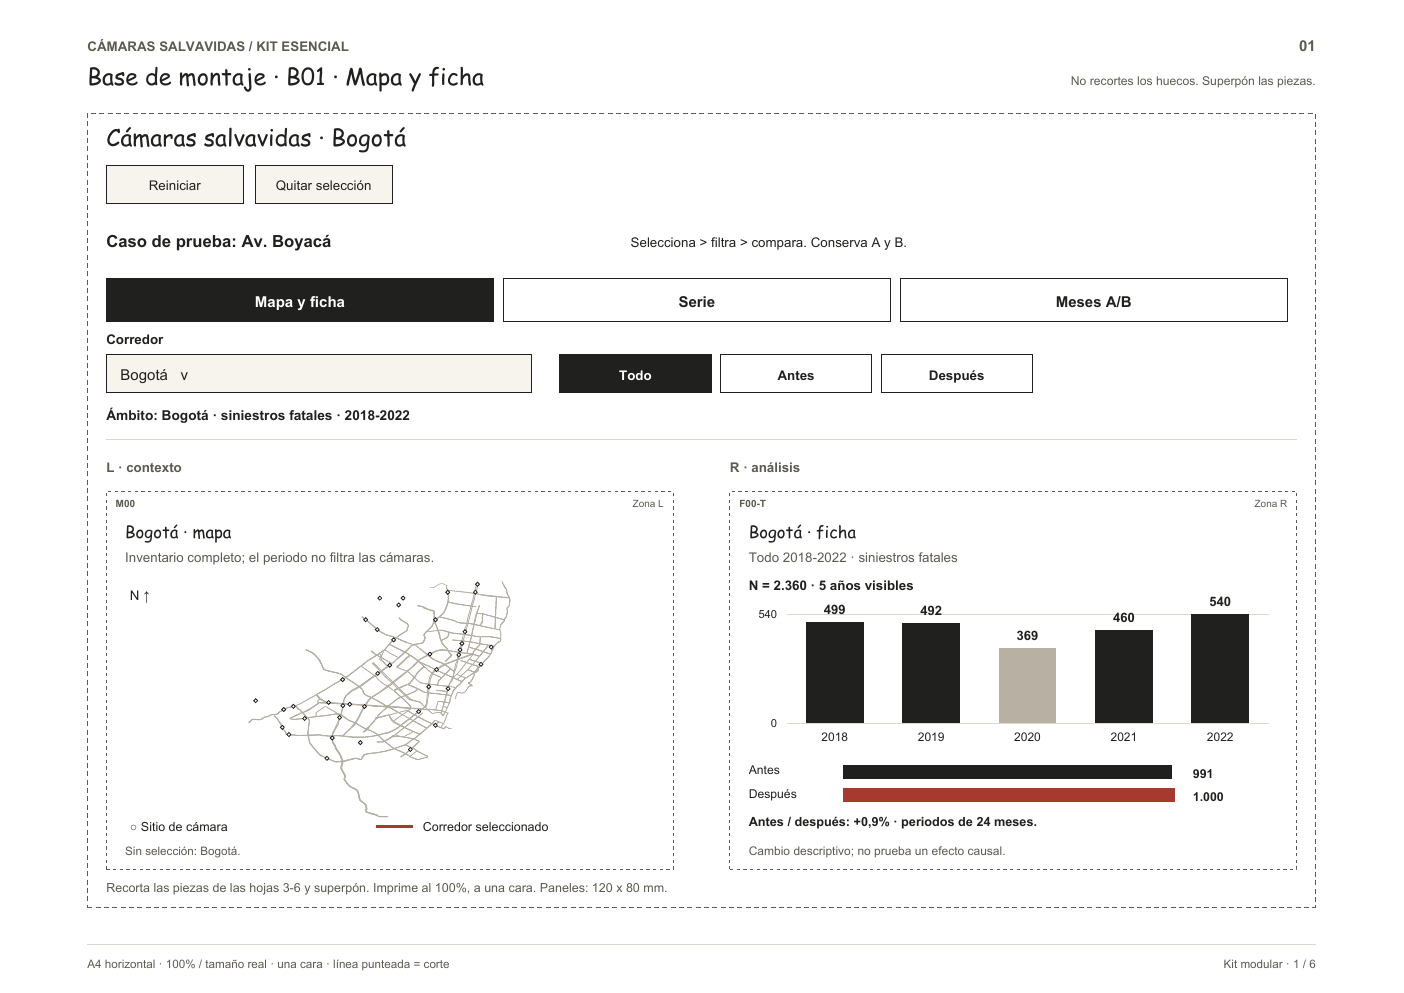
\includegraphics[width=0.49\linewidth]{paper-1}\hfill
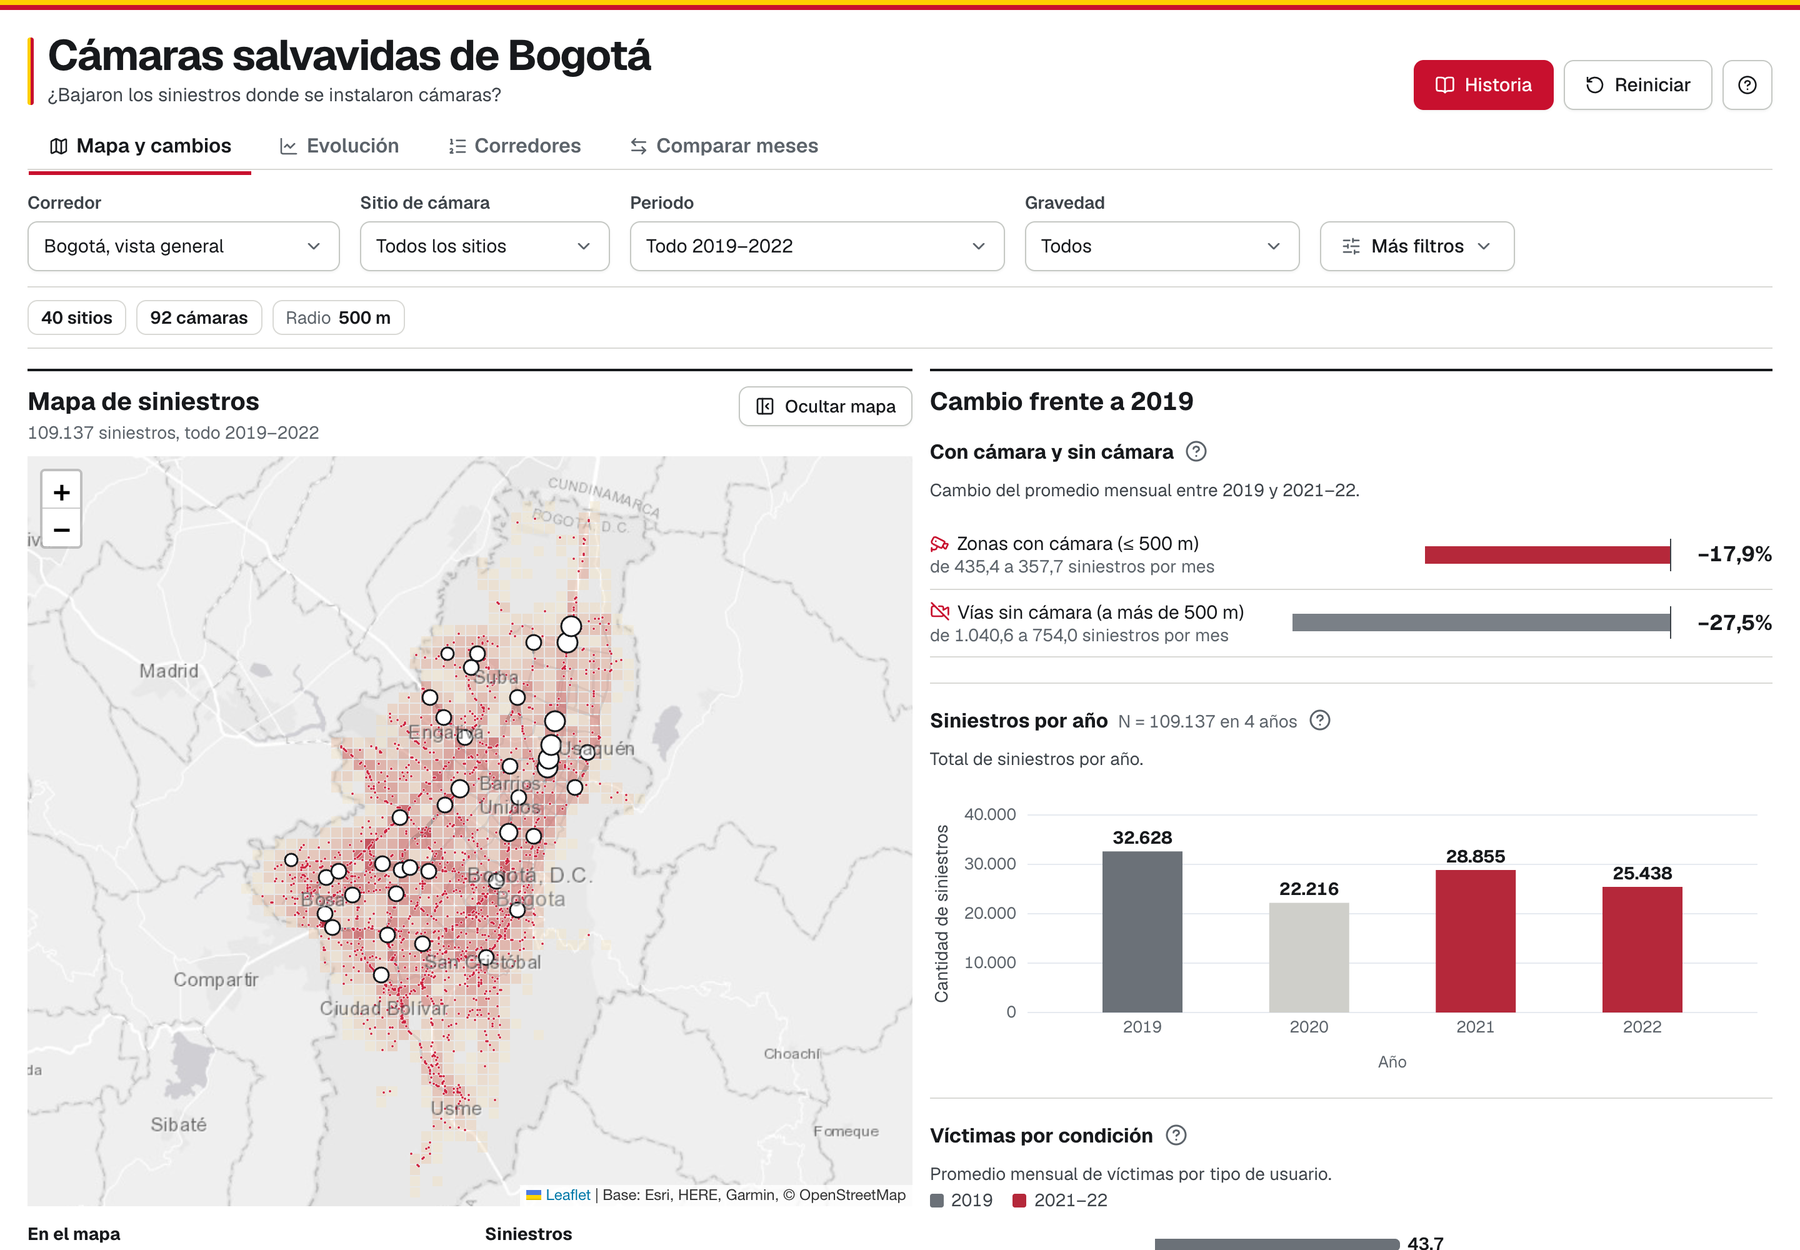
\includegraphics[width=0.49\linewidth]{it3}
\caption{Base de montaje del mapa y la ficha, y la vista Mapa y cambios}
\end{figure}

Al elegir la Av. Boyacá se reemplazaban el mapa y la ficha por las piezas de la hoja 4, con el corredor en rojo. Con eso probamos que la selección se entendiera como un estado que se conserva al cambiar de vista, y en el dashboard se mantiene igual, con el corredor resaltado, las demás cámaras atenuadas y un botón para quitar la selección en el mismo mapa. Lo que cambió es el mapa, que pasó de líneas sin contexto a un mapa base gris, y los siniestros, que ahora se ven como densidad o como puntos según el zoom.

\begin{figure}[H]\centering
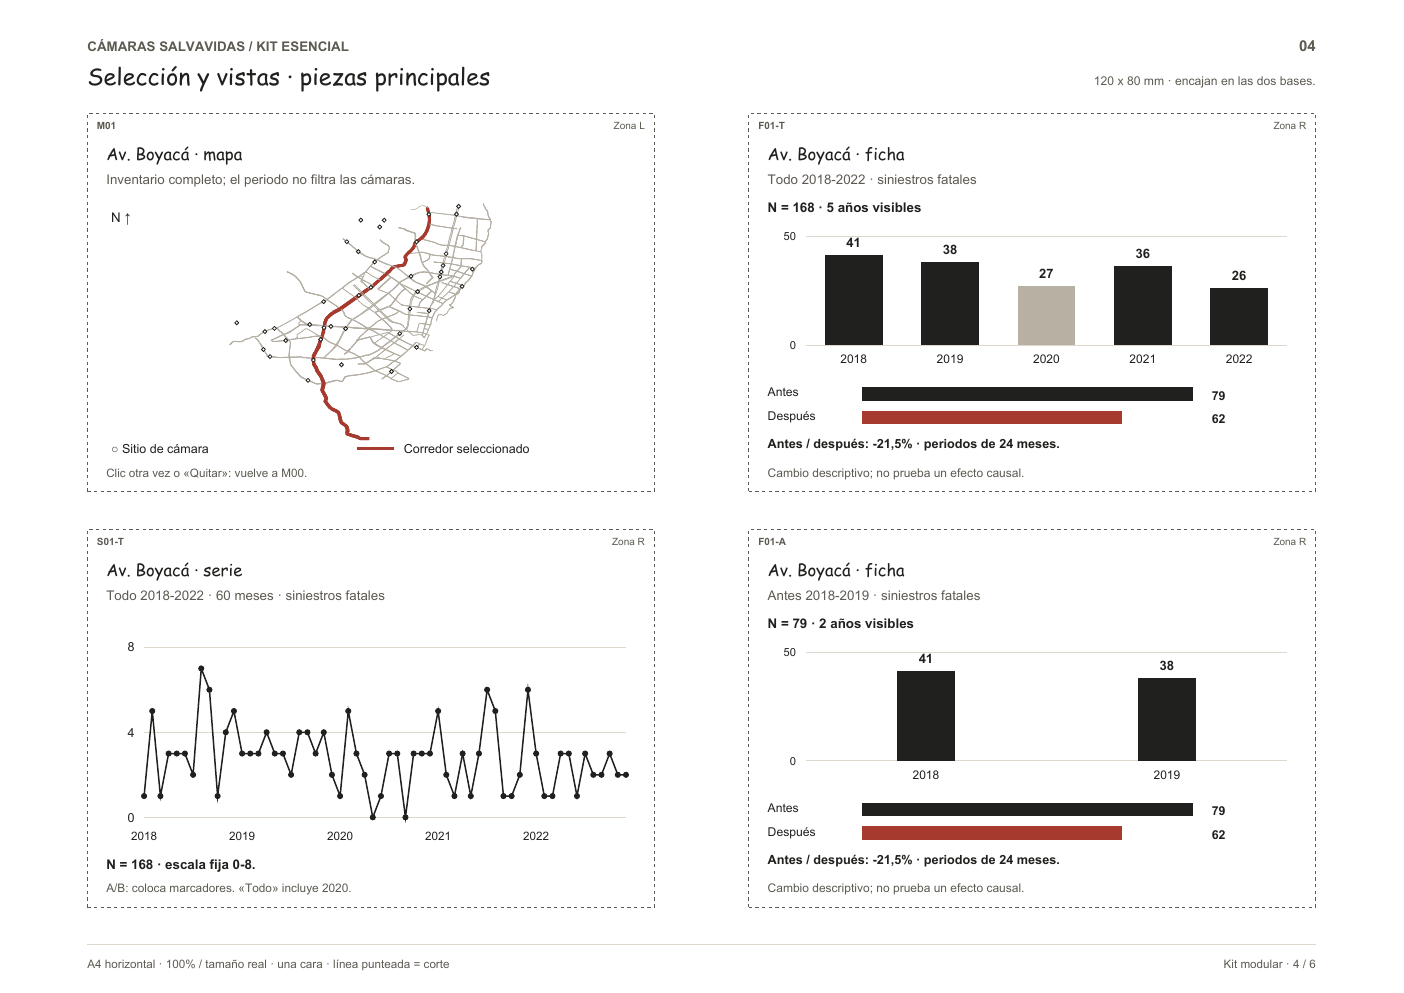
\includegraphics[width=0.49\linewidth]{paper-4}\hfill
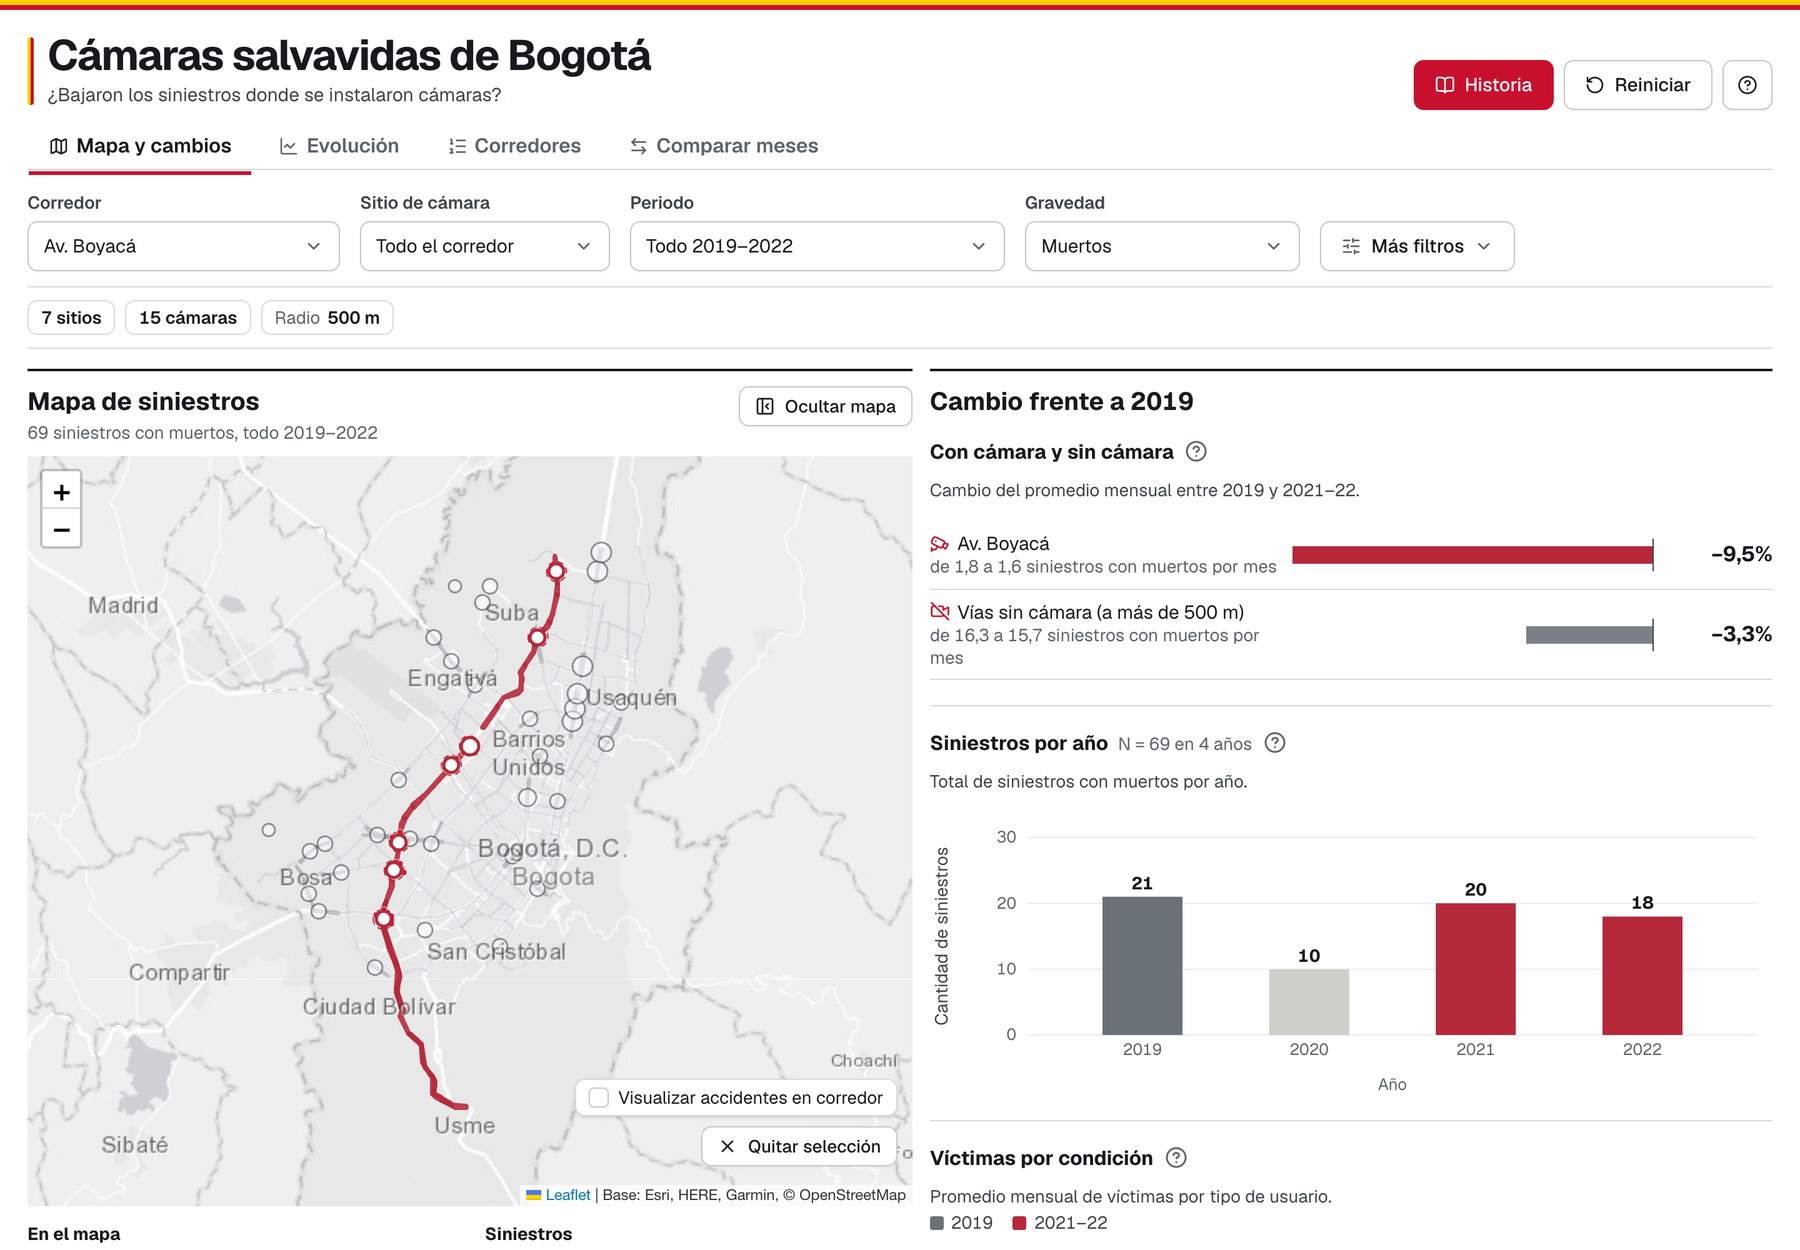
\includegraphics[width=0.49\linewidth]{ex_boyaca}
\caption{Selección de la Av. Boyacá en papel y en el dashboard}
\end{figure}

La serie en papel mostraba 60 meses de un corredor con una escala fija de 0 a 8, y los botones de antes y después la cambiaban por las piezas de la hoja 5. Con tan pocos siniestros fatales por mes la línea era puro zigzag y no había contra qué leerla, por lo que en la versión final la serie abre con todos los siniestros, tiene el promedio de 2019 como referencia, marca la instalación, la pandemia y las multas y deja acercar un periodo arrastrando, en lugar de depender de tres estados fijos.

\begin{figure}[H]\centering
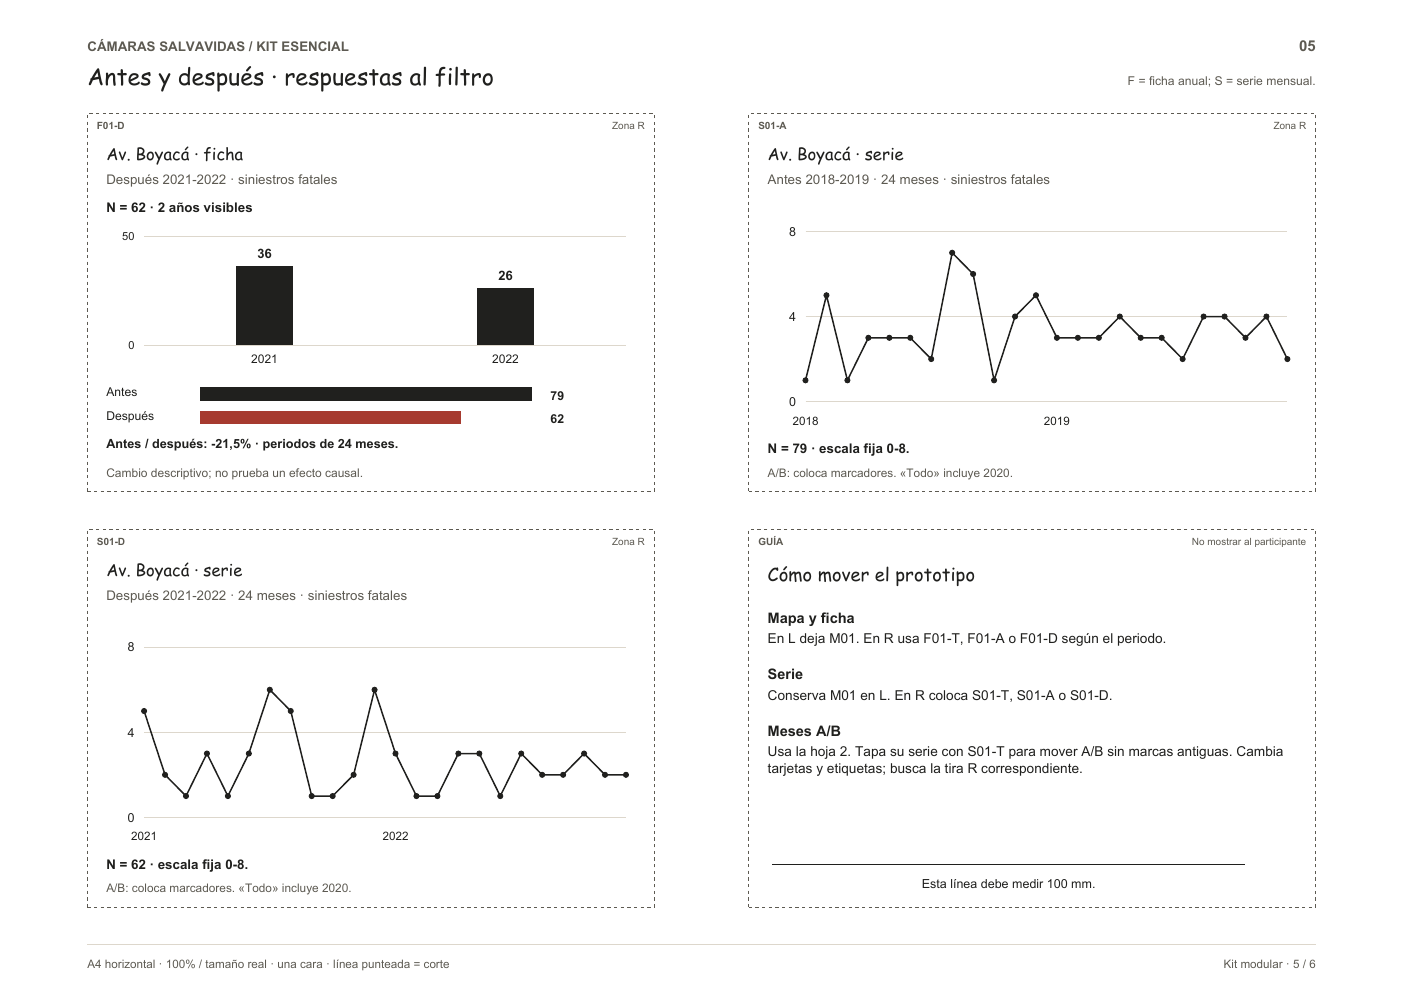
\includegraphics[width=0.49\linewidth]{paper-5}\hfill
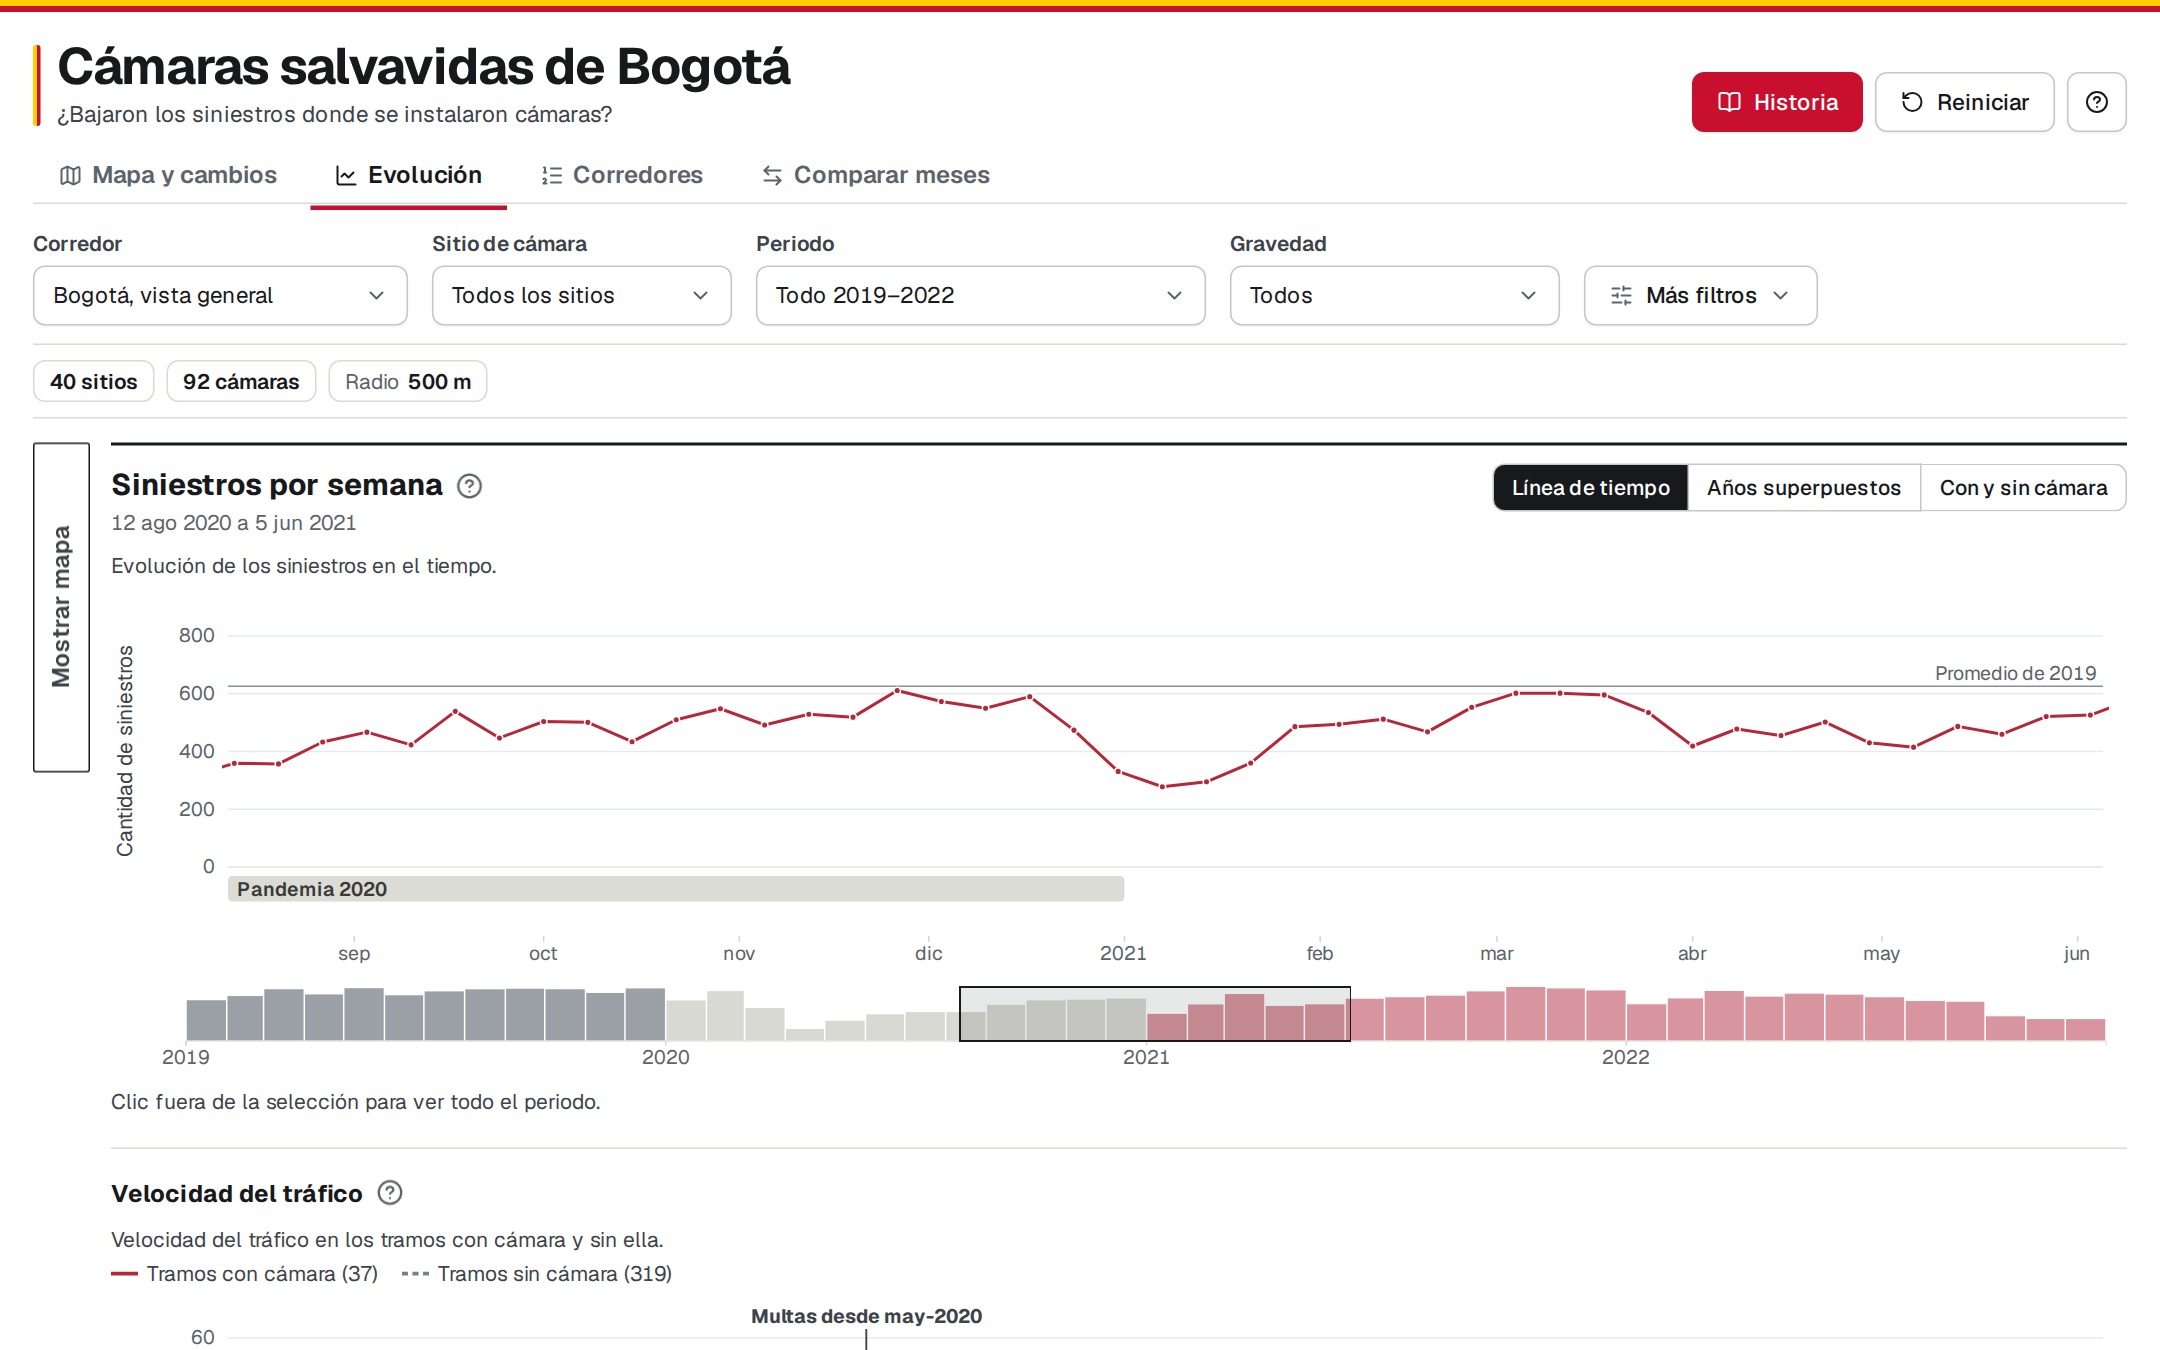
\includegraphics[width=0.49\linewidth]{ex_semanas}
\caption{Respuestas al filtro de periodo en papel y serie con zoom en el dashboard}
\end{figure}

La comparación A/B permitía elegir entre tres meses (noviembre de 2019, 2021 y 2022), mover las marcas sobre la serie y superponer las tarjetas con Bogotá y la Av. Boyacá. De esa prueba salió que la comparación necesitaba su propia pantalla y que un solo mes tiene demasiado ruido, así que ahora es la pestaña Comparar meses, sin mapa, donde cada lado es un grupo de meses que se elige con clic o arrastre y se compara como promedio mensual, con filas para siniestros, víctimas, cámaras instaladas y velocidad.

\begin{figure}[H]\centering
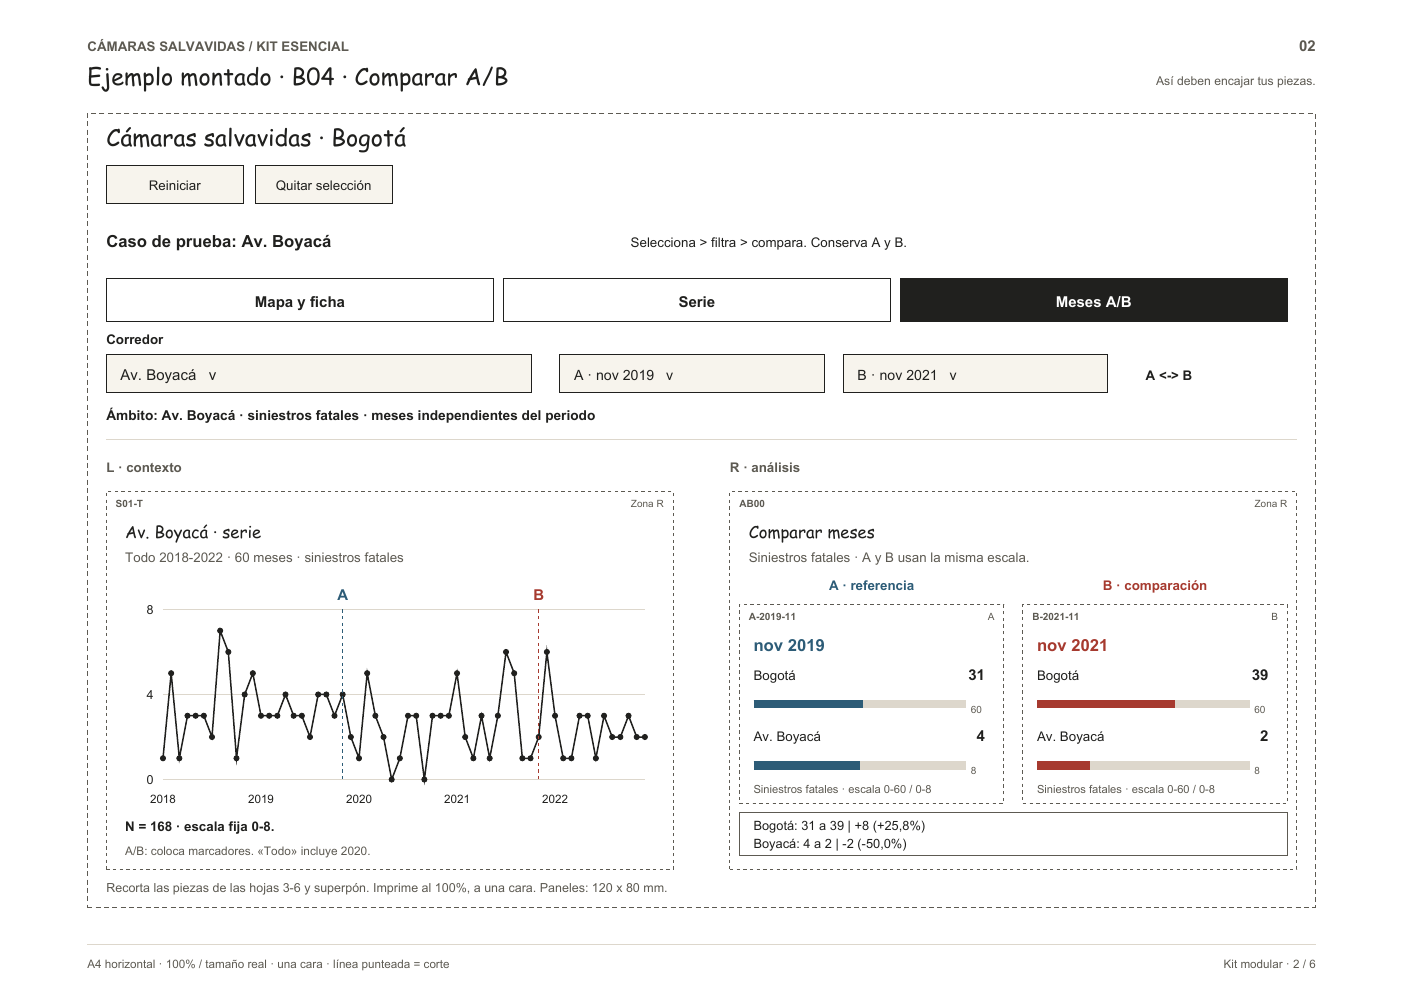
\includegraphics[width=0.49\linewidth]{paper-2}\hfill
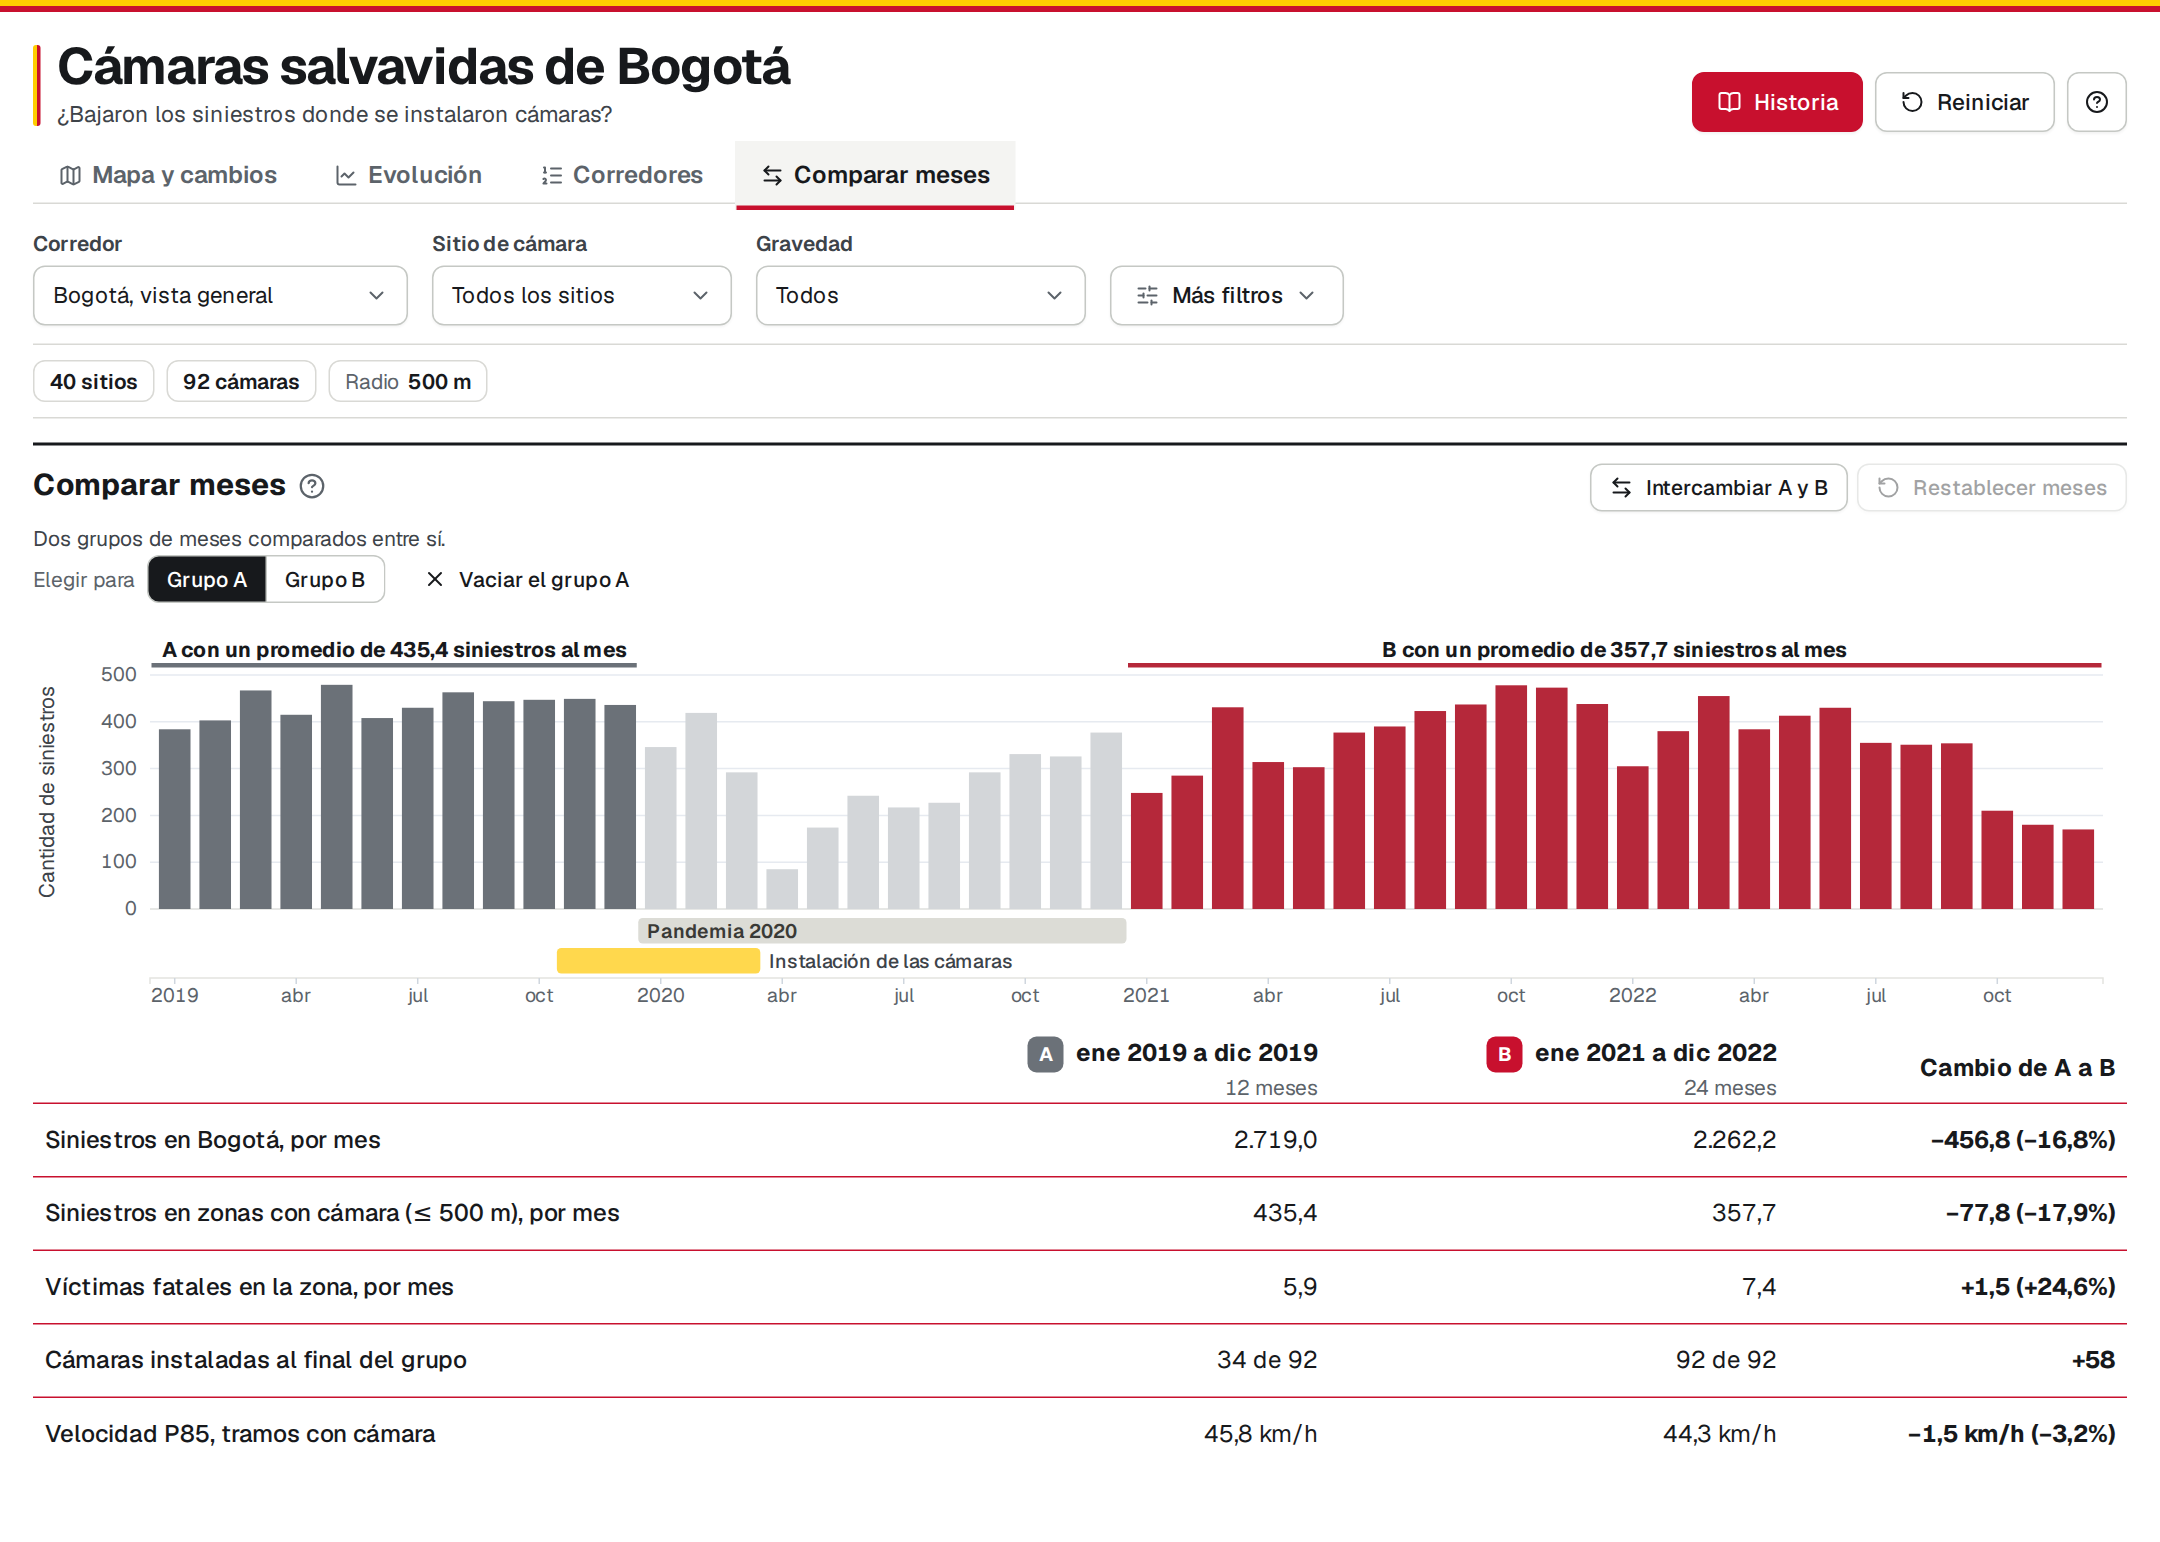
\includegraphics[width=0.49\linewidth]{v_ab}
\caption{Comparación A/B en papel y vista Comparar meses}
\end{figure}

Las piezas recortables mostraban además lo que esperábamos de la interacción, como la tarjeta que aparecía al pasar por un corredor con sus 15 cámaras y 168 siniestros fatales. Esa tarjeta decía ``Clic para seleccionar'', y en la versión final los tooltips dan solo datos porque una instrucción dentro de ellos confundía. Los marcadores A en azul y B en rojo pasaron a gris y rojo, para que el color signifique lo mismo que en el resto del dashboard.

\begin{figure}[H]\centering
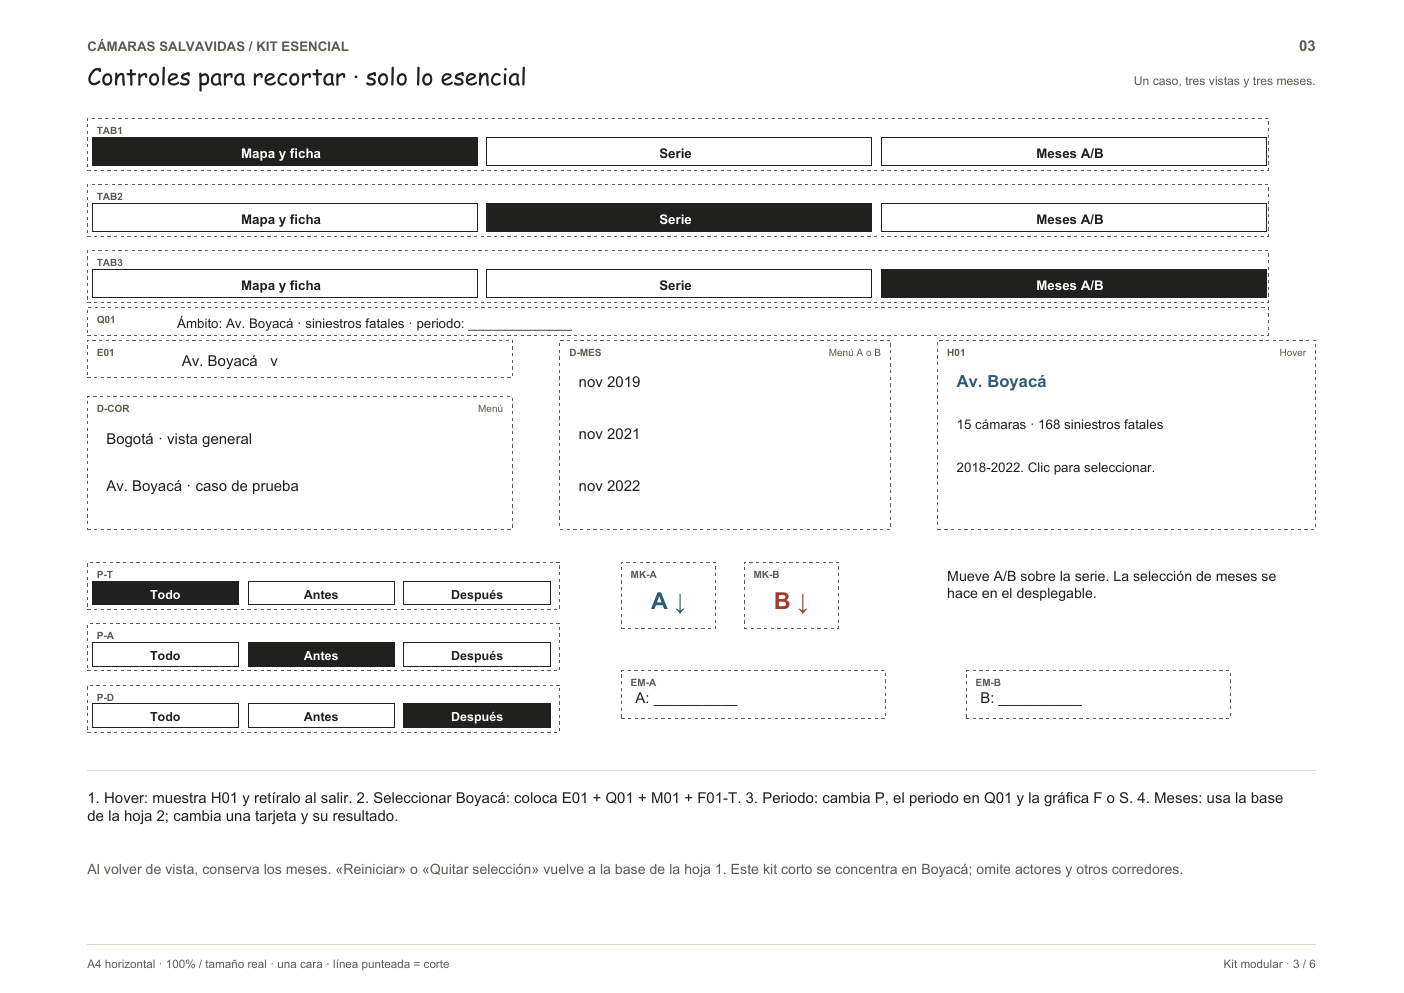
\includegraphics[width=0.49\linewidth]{paper-3}\hfill
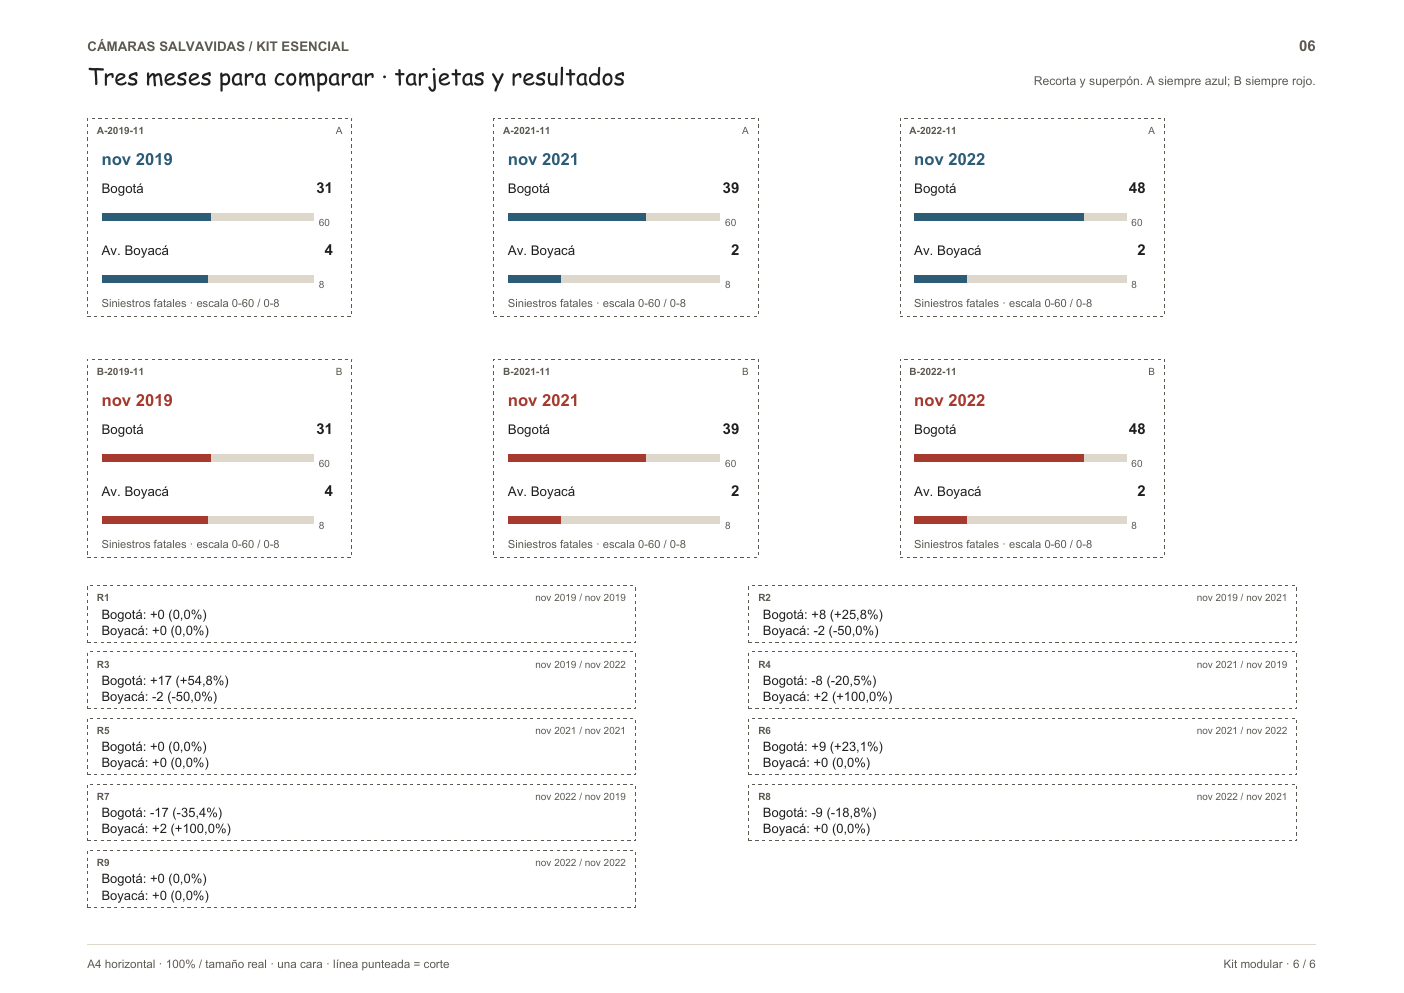
\includegraphics[width=0.49\linewidth]{paper-6}
\caption{Controles para recortar y tarjetas de los meses}
\end{figure}

\subsection{La versión final}

Además de lo que ya estaba en el papel, el dashboard sumó una pantalla de entrada, que respondió a la sugerencia de un tutorial y muestra la serie real de la ciudad, cuatro cifras y los caminos para empezar, con las preguntas en una ventana superpuesta desde la que cada una lleva a la vista que la responde. Las otras dos cosas que no existían en papel son la vista de Corredores, que permite encontrar el que más mejora o empeora sin probarlos uno por uno, y la velocidad del tráfico, que entró a partir de la duda que quedó en los comentarios sobre si incluirla. Ambas responden preguntas secundarias, así que quedaron en vistas y secciones a las que se llega después del panorama.

\begin{figure}[H]\centering
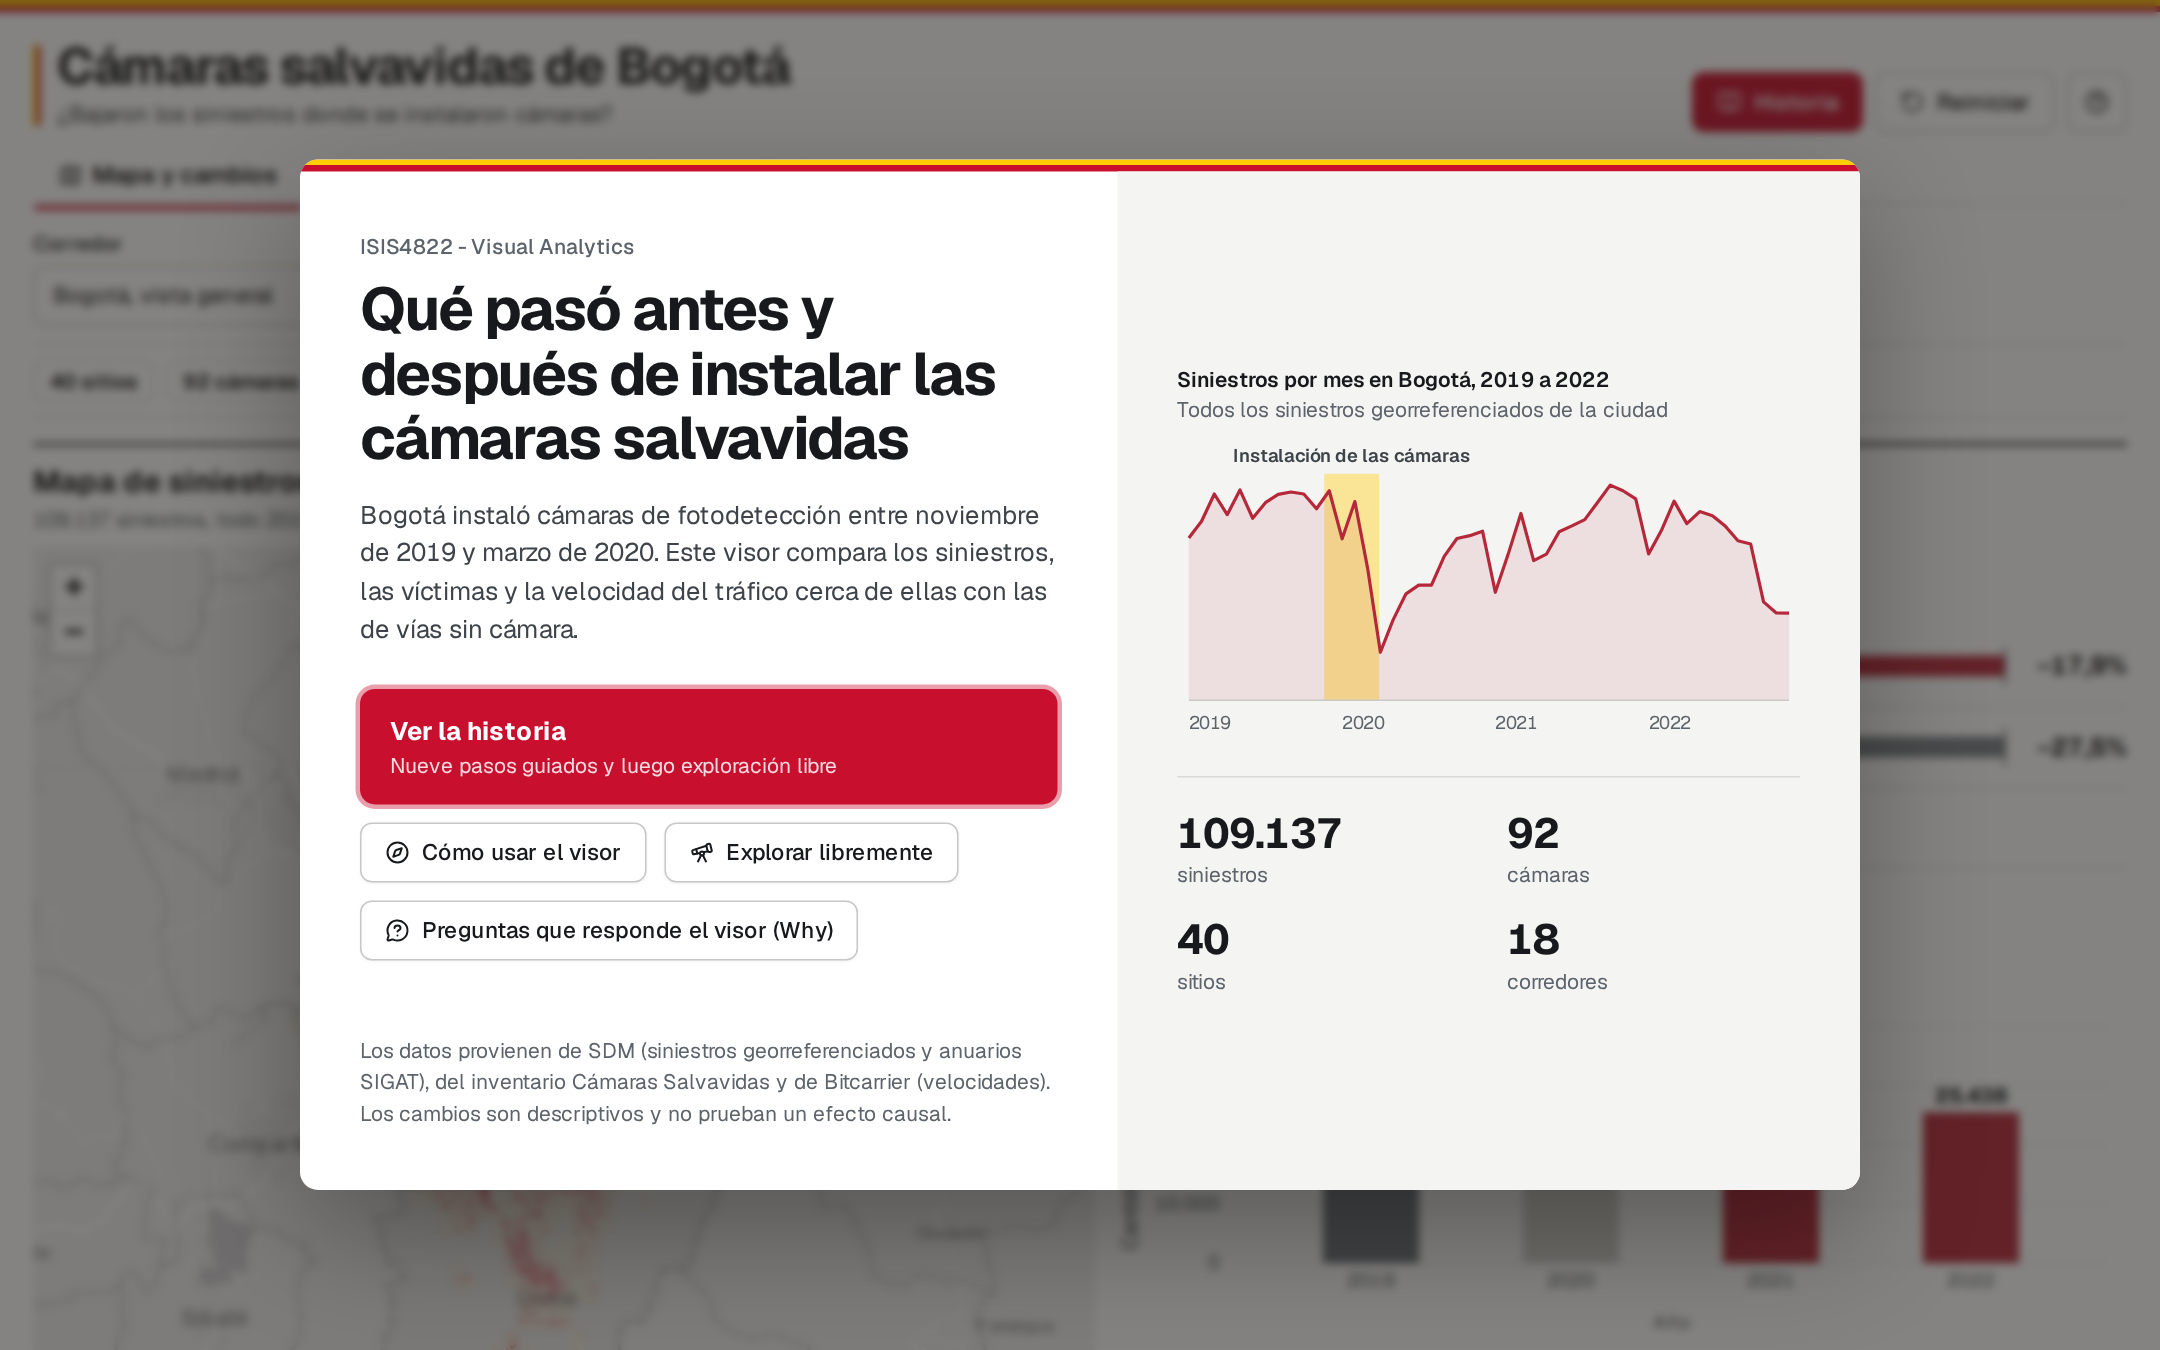
\includegraphics[width=0.49\linewidth]{inicio}\hfill
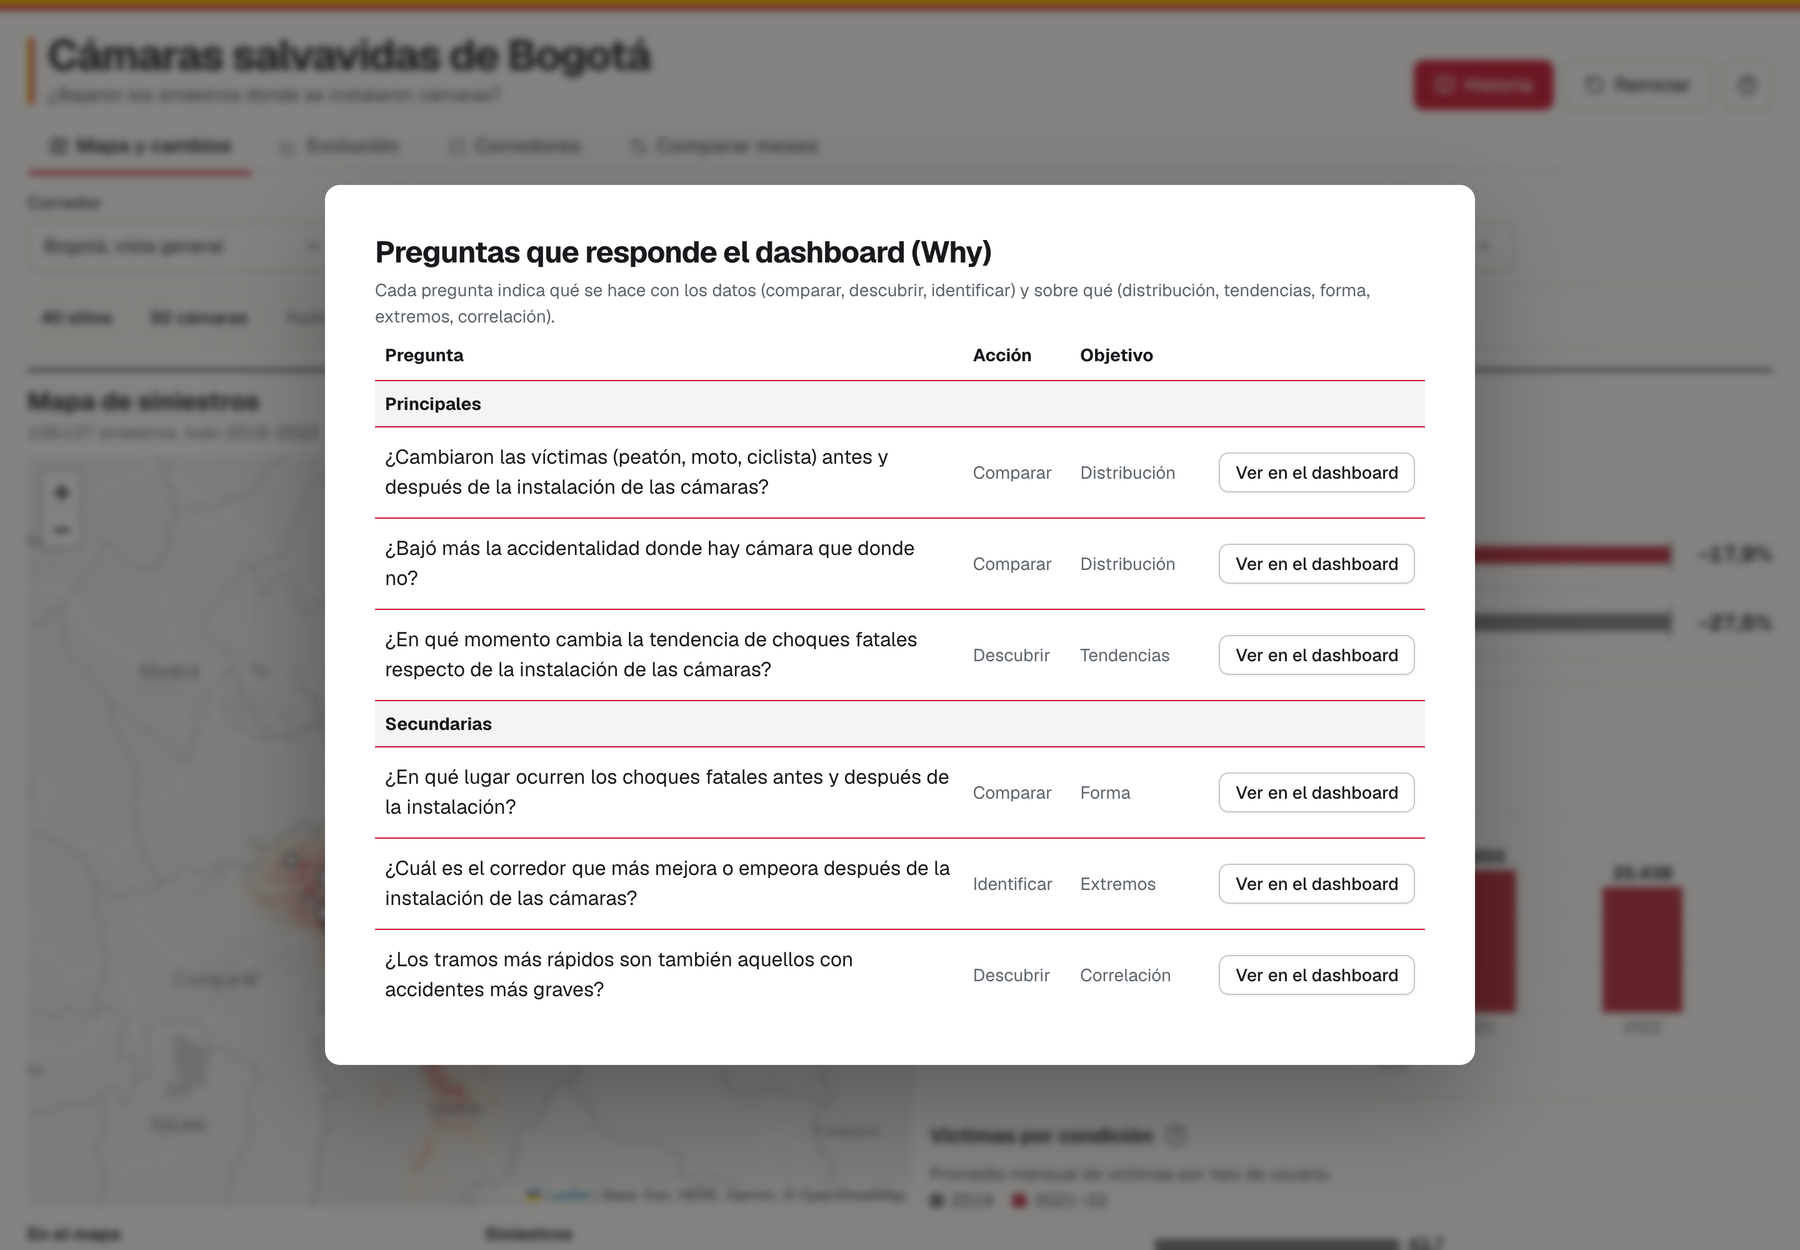
\includegraphics[width=0.49\linewidth]{preguntas}
\caption{Pantalla de inicio y ventana de preguntas}
\end{figure}

También pensamos la versión para celular, donde los filtros se agrupan en un botón. Los momentos por los que pasó la vista principal antes de llegar a esta se muestran en la última sección, junto con la evolución de las demás vistas.

\figura[0.3]{movil}{Vista en un celular}
\FloatBarrier
\section{Validaciones}


A principios de noviembre probamos el paper prototype descrito en la sección anterior y recogimos comentarios de otros grupos y notas del equipo, que respondimos como se muestra en la tabla. Los comentarios fueron útiles sobre todo porque apuntaban a cosas que nosotros no veíamos por conocer ya los datos, como la duda sobre si se tomaba toda la vía o un tramo, que nos mostró que el alcance de lo que se cuenta tenía que estar escrito y poder cambiarse. En dos casos hicimos un ajuste distinto al que nos pidieron, y la razón queda en la misma tabla.

\begin{table}[H]\centering\small
\begin{tabularx}{\linewidth}{P{5.4cm}Ll}
\toprule
\textbf{Comentario} & \textbf{Qué hicimos} & \textbf{Estado}\\
\midrule
Agregar filtros por tipo de siniestro, no solo fatales & Filtros de gravedad, tipo y actor. & Atendido\\
¿Se toma toda la vía o solo el tramo de la cámara? & Selector de sitio, radio y casilla para ver los siniestros del corredor. & Atendido\\
No dejar el mapa siempre fijo & Botón para ocultarlo. & Atendido\\
Pasar la comparación A/B a otra pantalla (grupo 2) & Pestaña propia, Comparar meses. & Atendido\\
Tutorial o pantalla de entrada (grupo 3) & Pantalla de inicio, recorrido e historia. & Atendido\\
Hover sobre la serie, por meses o días & Tooltips en la serie, con días solo al acercar. & Con ajuste\\
¿Incluir velocidad? & Gráfica aparte, para no usar un doble eje. & Con ajuste\\
Pintar varias líneas a la vez, antes y después & Años superpuestos y con y sin cámara. & Atendido\\
Conteo de cámaras y siniestros en la comparación & Filas de la tabla de Comparar meses. & Atendido\\
Quitar el mapa en ciertas circunstancias & Comparar meses no muestra mapa. & Atendido\\
\bottomrule
\end{tabularx}
\caption{Comentarios del paper prototype y respuesta}
\end{table}

Falta sumar a esta prueba las demás validaciones que hicimos, con quiénes participaron, qué tareas se les pidieron y qué cambio salió de cada hallazgo, para que se pueda seguir la relación entre lo que observamos y lo que decidimos.

\pendiente{Incorporar las demás estrategias de validación, sus participantes, tareas y hallazgos.}

\section{Storytelling}

El dashboard tiene cuatro vistas y varios filtros que se combinan, y eso sirve para quien ya sabe qué buscar, pero no para quien llega por primera vez y quiere saber si las cámaras sirvieron. La respuesta que podemos dar además no cabe en una cifra, porque depende de con qué se compare, de qué gravedad se mire y de cómo se lea 2020, así que necesitábamos una forma de contar primero esas condiciones y solo después dejar que cada persona explorara.

Segel y Heer describen la narración con visualizaciones como un punto entre dos extremos, uno en el que el autor lleva al lector paso a paso y otro en el que el lector decide qué mirar, y proponen estructuras que mezclan los dos, de las cuales comparamos tres antes de escoger.

\begin{table}[H]\centering\small
\begin{tabularx}{\linewidth}{P{3.6cm}LL}
\toprule
\textbf{Estructura} & \textbf{Qué ofrece} & \textbf{Por qué no bastaba sola o por qué se eligió}\\
\midrule
Copa de martini & Un tramo guiado y después exploración abierta. & Fue la elegida, porque primero da contexto y luego libertad.\\
Presentación interactiva & Diapositivas con interacción dentro de cada una. & Mantiene al lector dentro del guion y limita a quien quiere analizar.\\
De lo general a lo particular (drill-down) & Una vista general desde la que el lector elige. & No garantiza que se vean las advertencias antes de sacar conclusiones.\\
\bottomrule
\end{tabularx}
\caption{Estructuras consideradas}
\end{table}

La copa de martini era la mejor opción para nosotros porque pone los dos momentos en el orden que necesitábamos. El tallo es un recorrido angosto en el que fijamos la vista, los filtros y el texto, de modo que todos ven la referencia sin cámara y la advertencia sobre 2020 antes de sacar una conclusión, y la copa se abre cuando esa base ya está puesta. Una presentación interactiva habría mantenido al lector dentro del guion hasta el final, y Carolina, que quiere armar su propio antes y después, se habría quedado sin hacerlo. Un recorrido de lo general a lo particular tiene el problema contrario, porque deja elegir desde el principio y con tantos filtros es fácil terminar en la combinación que confirma lo que uno ya pensaba, sin pasar por las advertencias.

También la preferimos por la forma en que se reparten los perfiles. Diana entra casi siempre desde el celular, desde un enlace, y tiene poca experiencia leyendo datos, por lo que necesita un hilo que le diga qué está viendo en cada paso. Andrés busca el corredor que empeoró, y el tallo lo lleva hasta allí pasando por el contexto que su artículo necesita, mientras que Carolina puede recorrerlo en poco tiempo o saltarlo e ir directo a los filtros, así que una sola estructura les sirve a los tres sin hacer una versión para cada uno. La idea de una secuencia guiada ya estaba en los wireframes por pasos, y la copa de martini nos dio la forma de cerrarla con libertad en lugar de terminar en el último paso.

La historia quedó en nueve pasos guiados y un décimo de exploración libre. Se inspira en las preguntas sin repetirlas, y el orden va de lo que el lector necesita saber primero a lo que puede concluir. Cada paso fija una sola idea y mueve el dashboard a la vista que la muestra, en lugar de usar diapositivas aparte, porque así el lector aprende dónde está cada cosa mientras sigue el relato y cuando la historia termina ya sabe volver a ella.

\begin{table}[H]\centering\small
\begin{tabularx}{\linewidth}{cP{4.8cm}L}
\toprule
\textbf{Paso} & \textbf{Título} & \textbf{Por qué va ahí}\\
\midrule
1 & Dónde están las cámaras & Ubica al lector y presenta la referencia antes de mostrar cifras.\\
2 & Un quiebre en 2020 & Advierte sobre 2020 antes de comparar.\\
3 & Cerca y lejos de las cámaras & Es la comparación central.\\
4 & Peatones, motociclistas y ciclistas & Pasa de los siniestros a las personas.\\
5 & Antes y después en el mapa & Lleva el cambio al lugar.\\
6 & Corredores que se separan & Muestra que el total esconde diferencias.\\
7 & Velocidad y gravedad & Explora un posible mecanismo.\\
8 & Lo que los datos no dicen & Pone los límites antes de la conclusión.\\
9 & Lo que sí se puede decir & Cierra con una afirmación acotada.\\
10 & Ahora, a explorar & Abre la copa con accesos a las vistas.\\
\bottomrule
\end{tabularx}
\caption{Pasos de la historia}
\end{table}

\begin{figure}[H]\centering
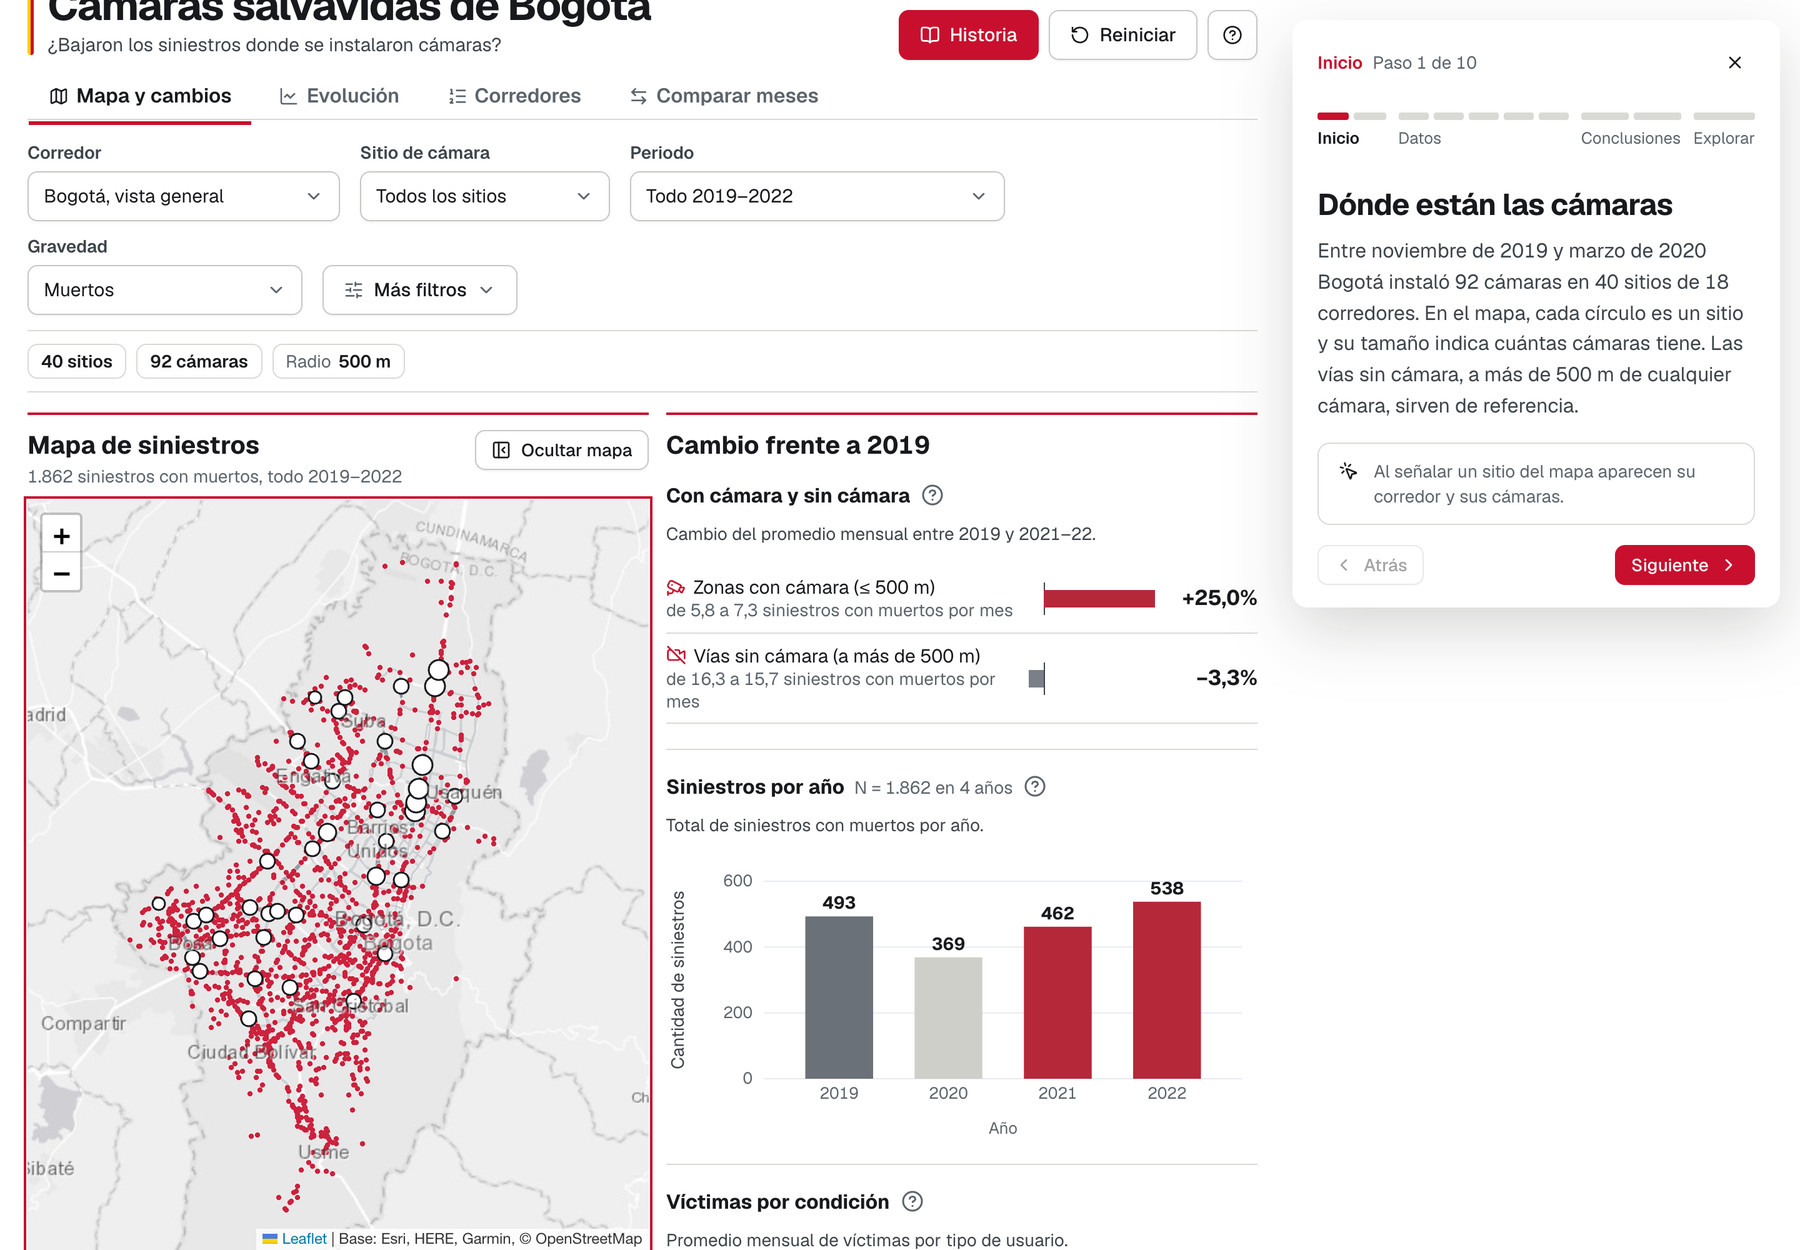
\includegraphics[width=0.49\linewidth]{h1}\hfill
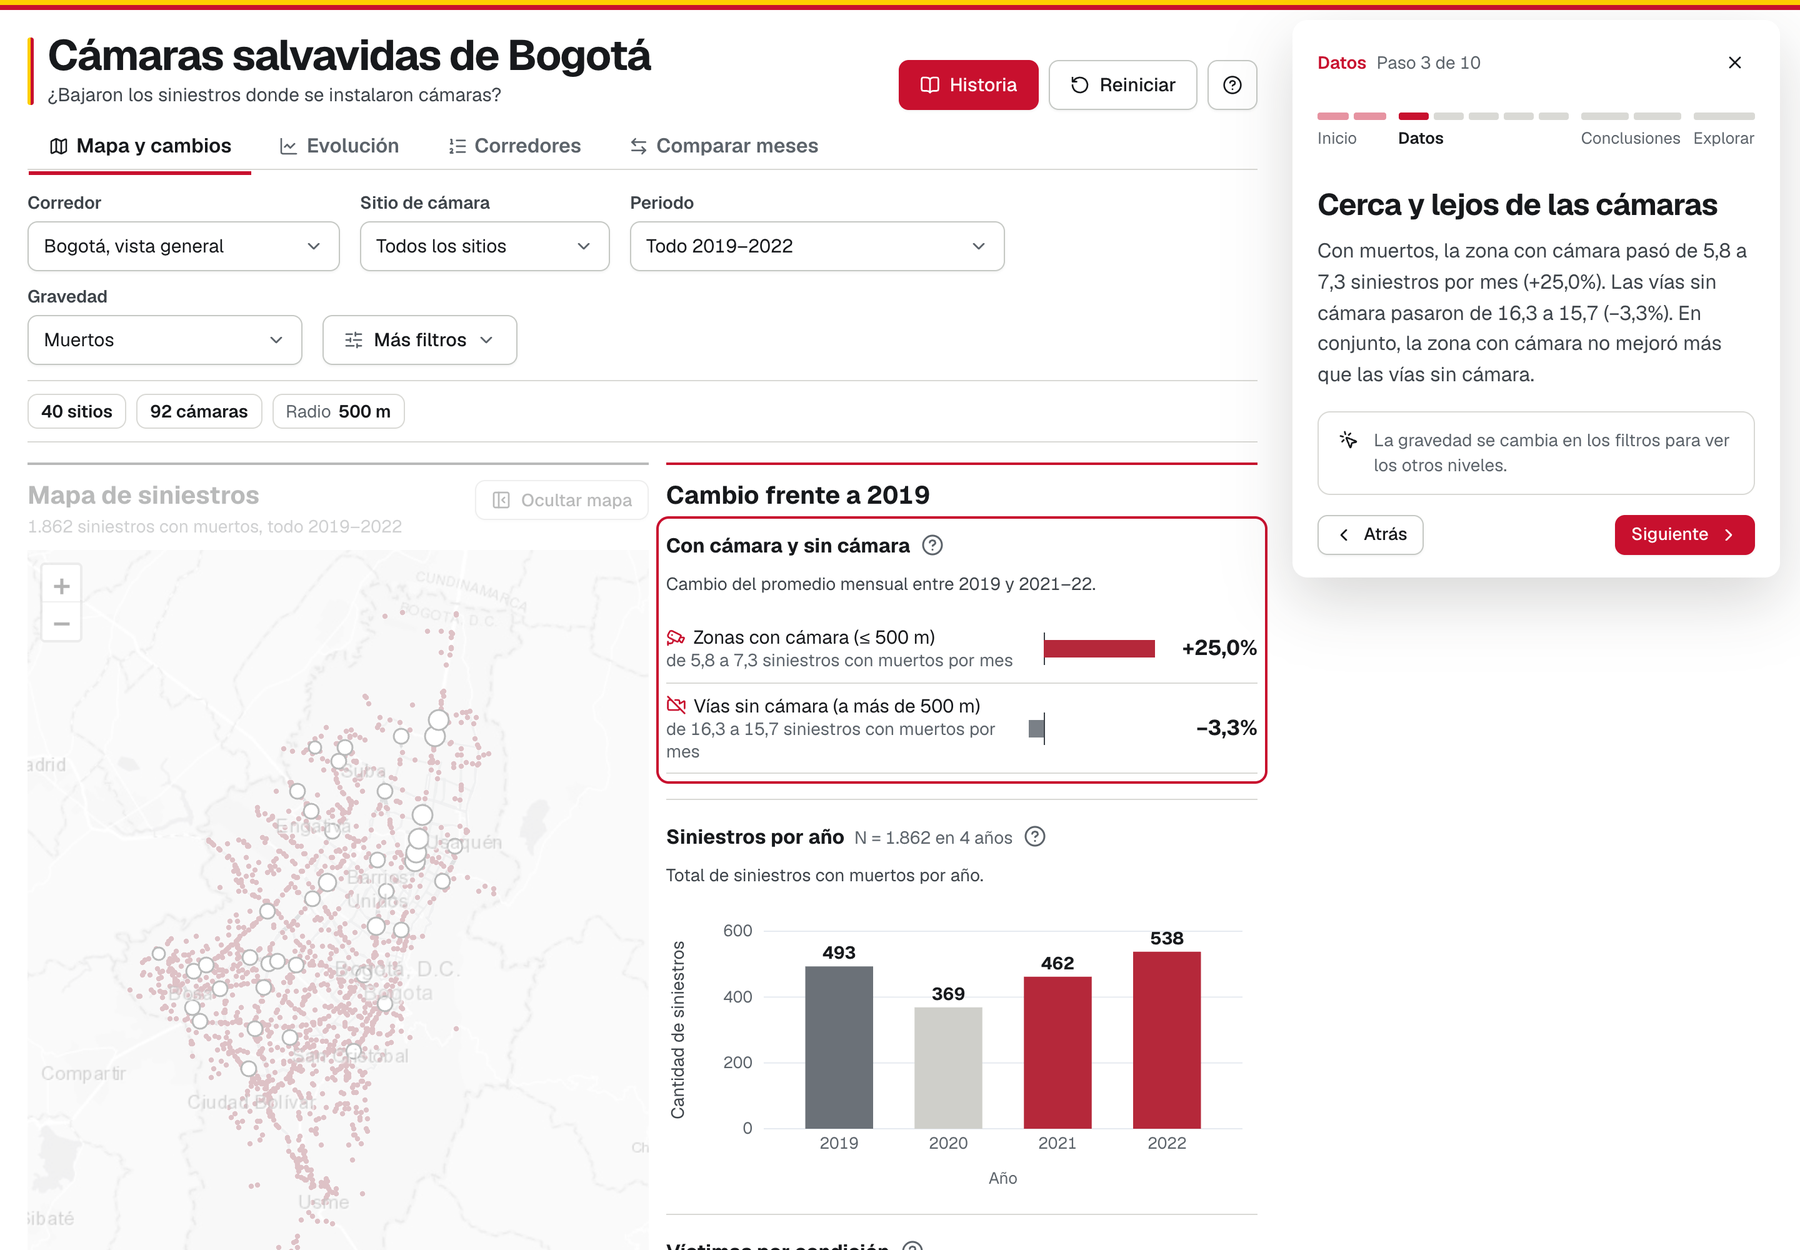
\includegraphics[width=0.49\linewidth]{h3}\par\smallskip
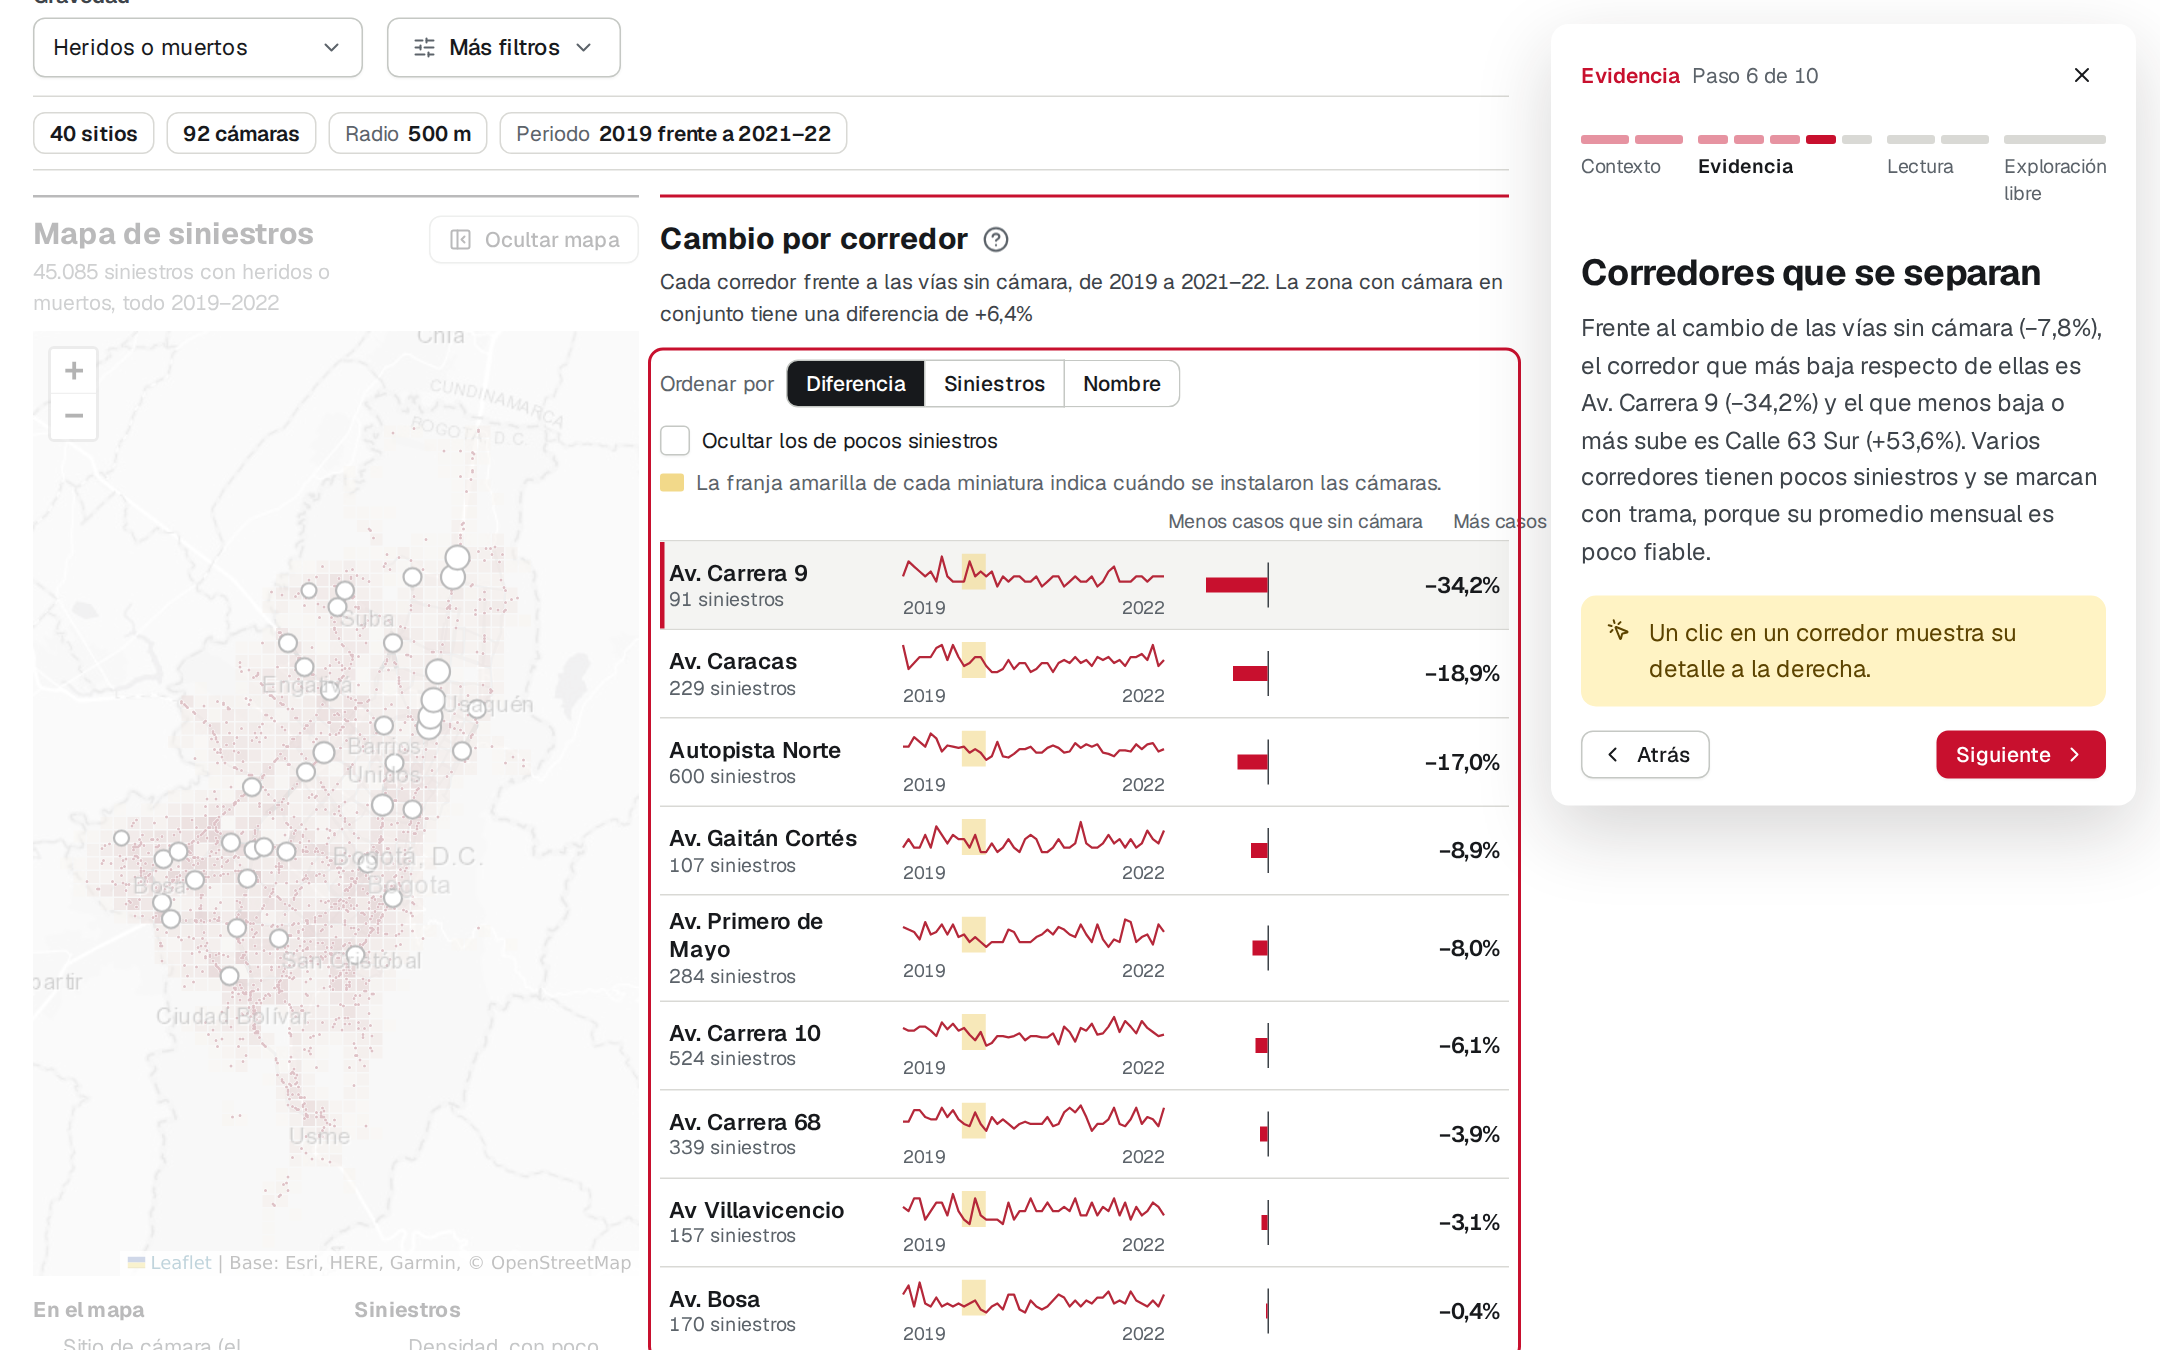
\includegraphics[width=0.49\linewidth]{h6}\hfill
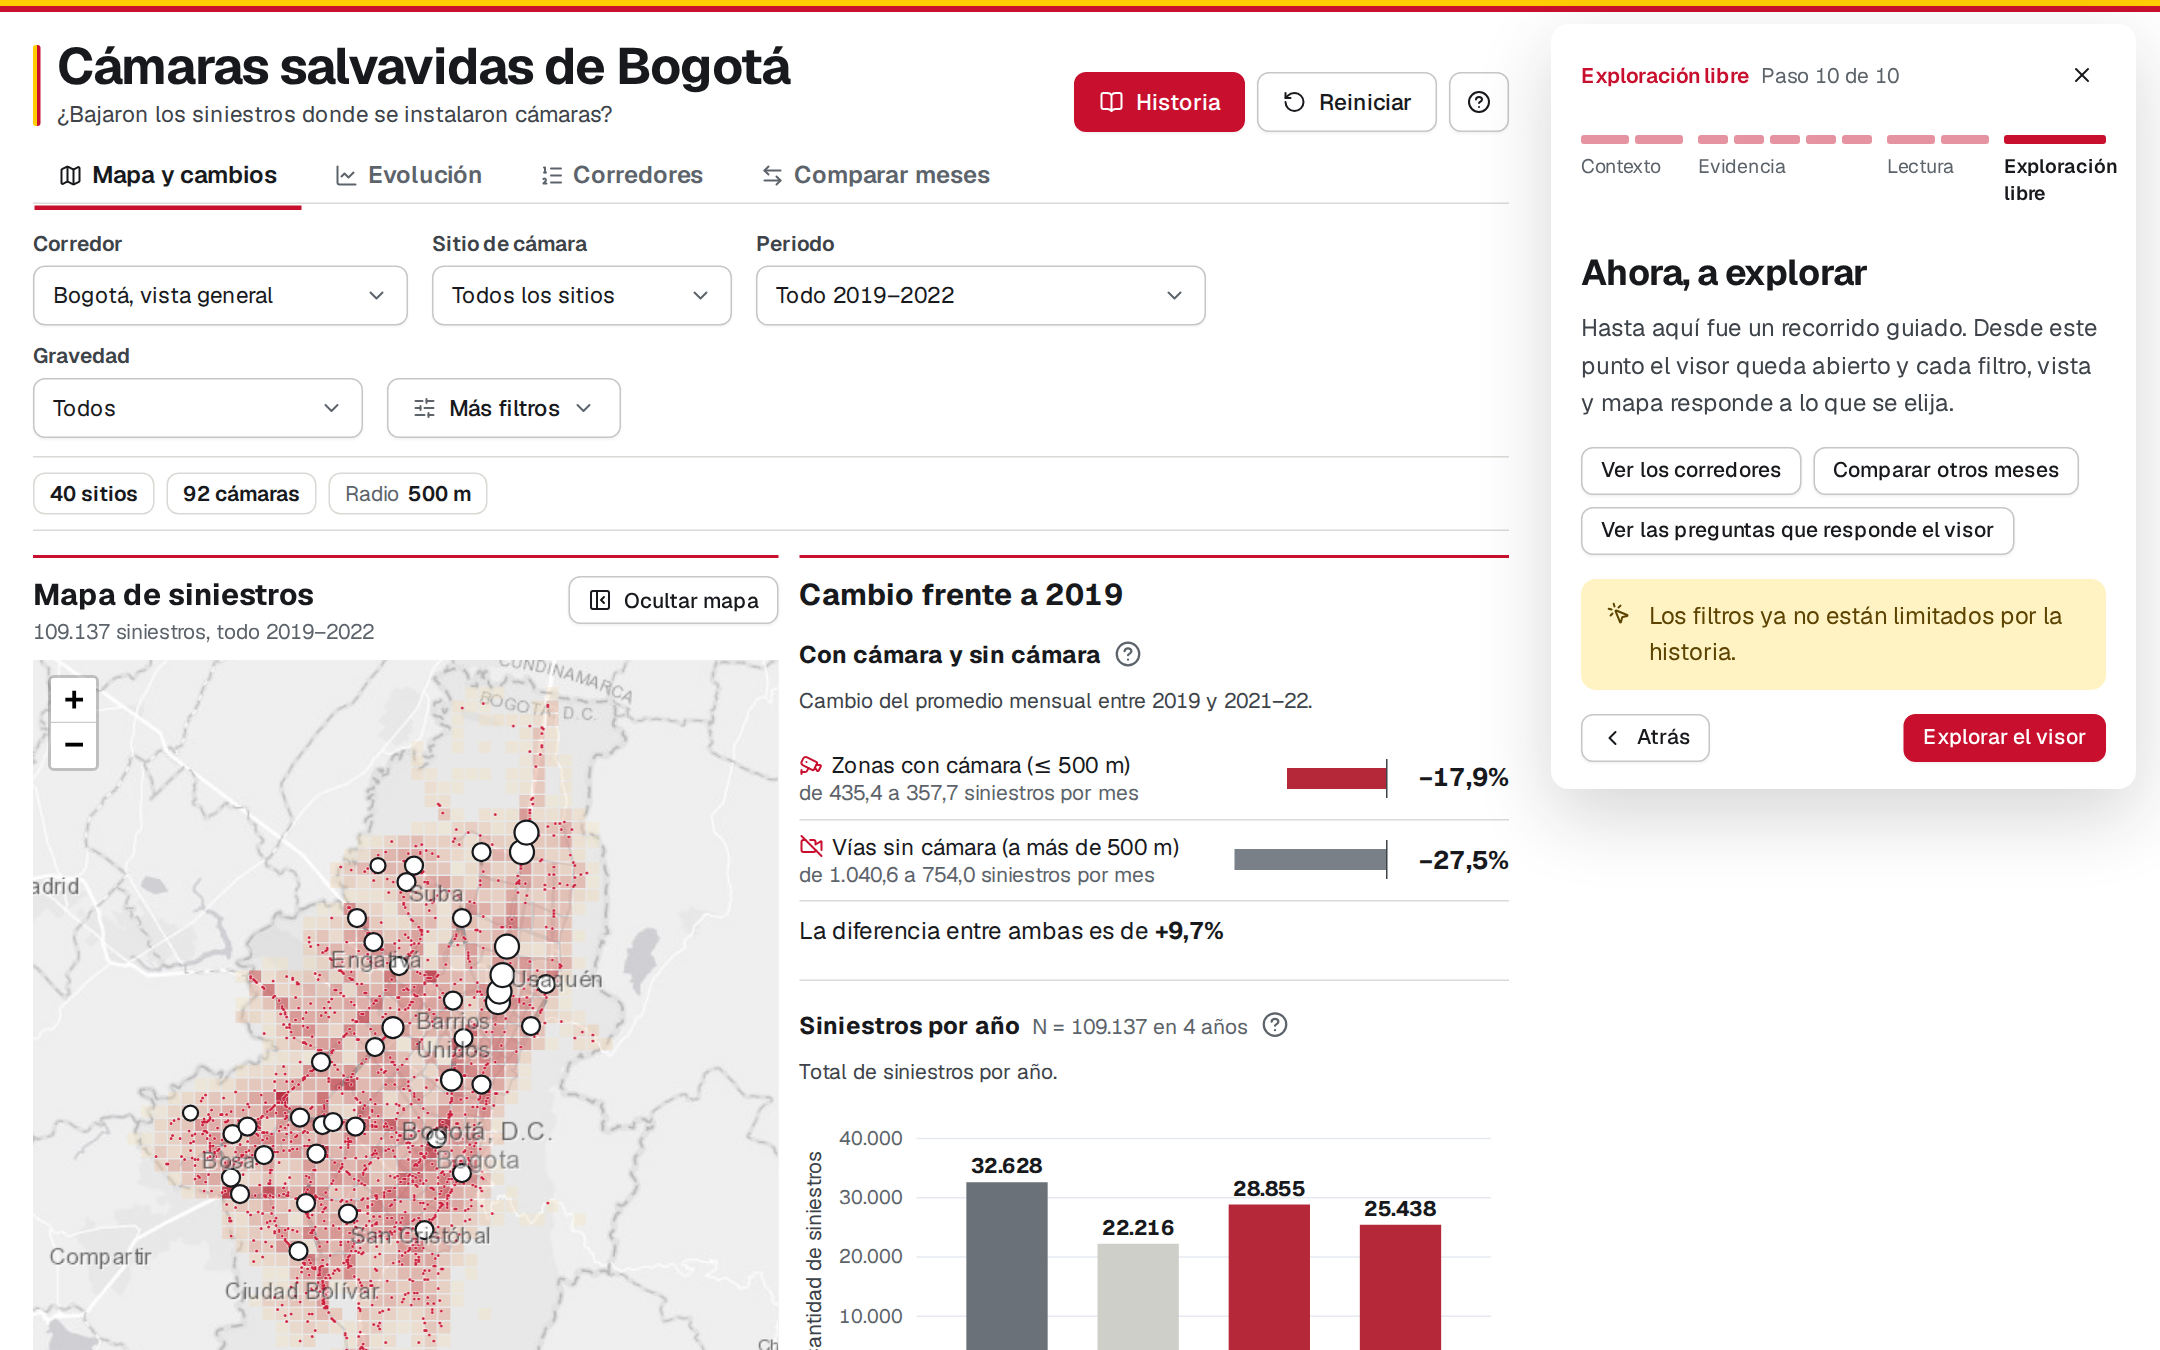
\includegraphics[width=0.49\linewidth]{h10}
\caption{Pasos 1, 3, 6 y 10}
\end{figure}

Durante los pasos guiados limitamos los controles para que cada texto coincida con lo que se ve, calculamos las cifras con los datos cargados para que no queden desactualizadas y al terminar no reiniciamos el dashboard, de modo que la exploración arranca desde lo último que se mostró. Si alguien se sale del guion se lo avisamos en lugar de bloquearlo por completo, y puede cerrar la historia en cualquier momento, porque obligar a terminar nueve pasos a quien ya tiene claro lo que busca iría en contra de la razón por la que dejamos la exploración libre.

\clearpage
\section{Evolución del dashboard y consideraciones de diseño}

En esta sección contamos cómo estaba cada parte del dashboard, qué cambiamos y por qué, y buena parte de esos cambios salió de los comentarios del paper prototype. También hubo ideas que descartamos, como fusionar Comparar meses dentro de Evolución para quitar gráficas repetidas, que probamos y deshicimos. También quitamos la sección fija de preguntas al final de la página, porque alargaba el dashboard y pasó a una ventana de la pantalla de inicio, y el icono de cámara dibujado en el mapa, que se veía decorativo y cambiamos por un marcador geométrico.

\subsection{Cuatro momentos del dashboard}

El dashboard no salió de una sola vez, y mirar sus versiones internas ayuda a entender por qué la actual es como es. La primera tenía tres vistas, que eran Mapa y ficha, Serie y Meses A/B, con los filtros como botones, un fondo cálido, títulos con serifa y el azul y el rojo para el antes y el después, y abría mostrando solo los siniestros con muertos. Ya permitía seleccionar, filtrar y comparar, pero obligaba a leer una ficha apretada para encontrar la respuesta y no ofrecía ningún hilo a quien llegaba por primera vez.

En la segunda sumamos la historia guiada y una cuarta vista, Panorama, para ver los 18 corredores a la vez, porque probarlos uno por uno no respondía cuál mejoraba o empeoraba. También cambiamos el periodo y la gravedad a menús desplegables con nombres completos, como ``Antes de la instalación'', porque las etiquetas cortas no decían a qué se referían, y pasamos a un fondo más claro.

La tercera fue una reescritura de la interfaz en la que cambiamos los nombres de las pestañas, la tipografía y el color, usamos un solo acento verde azulado para quitar el aspecto genérico y, sobre todo, cambiamos la forma de comparar, con barras sobre una escala común y la referencia sin cámara en un primer plano. La versión actual toma esa base, le da la identidad de Bogotá y ajusta cada vista a partir de lo que seguía sin entenderse.

\begin{figure}[H]\centering
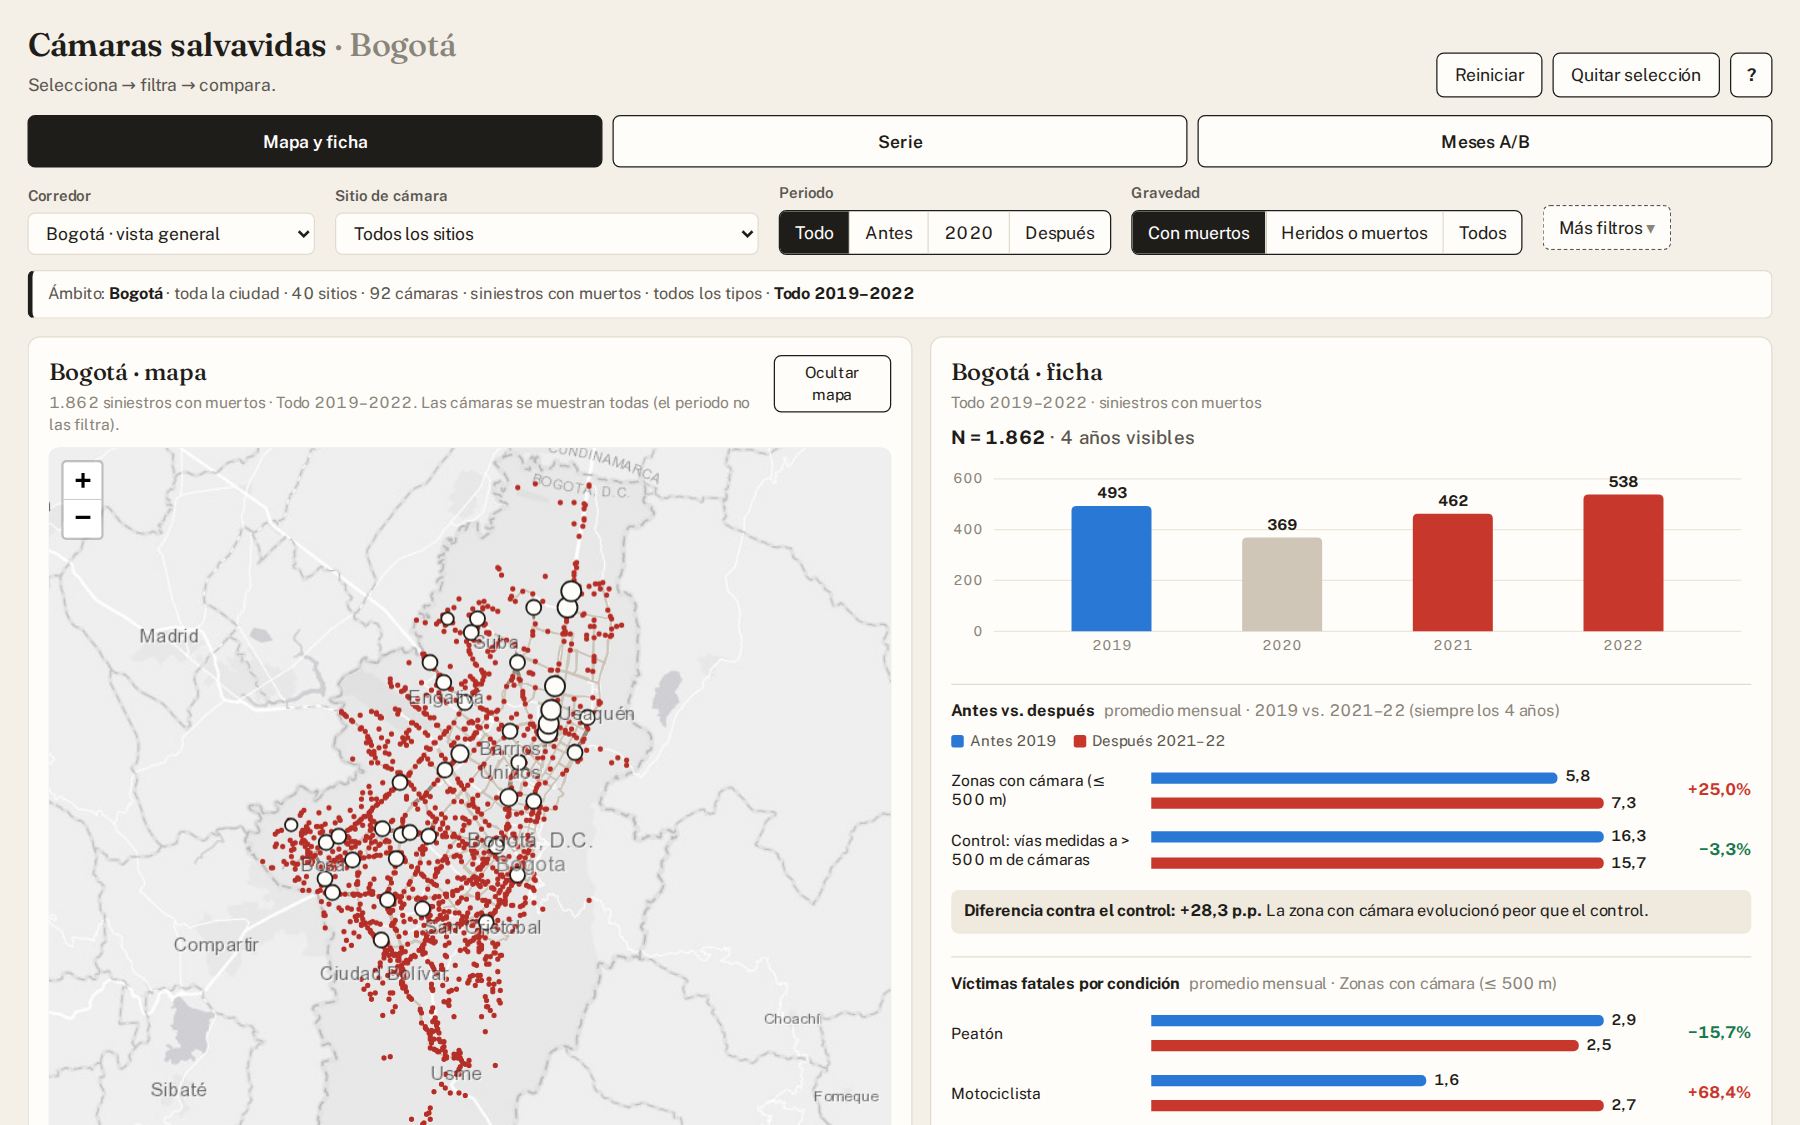
\includegraphics[width=0.49\linewidth]{v1_mapa}\hfill
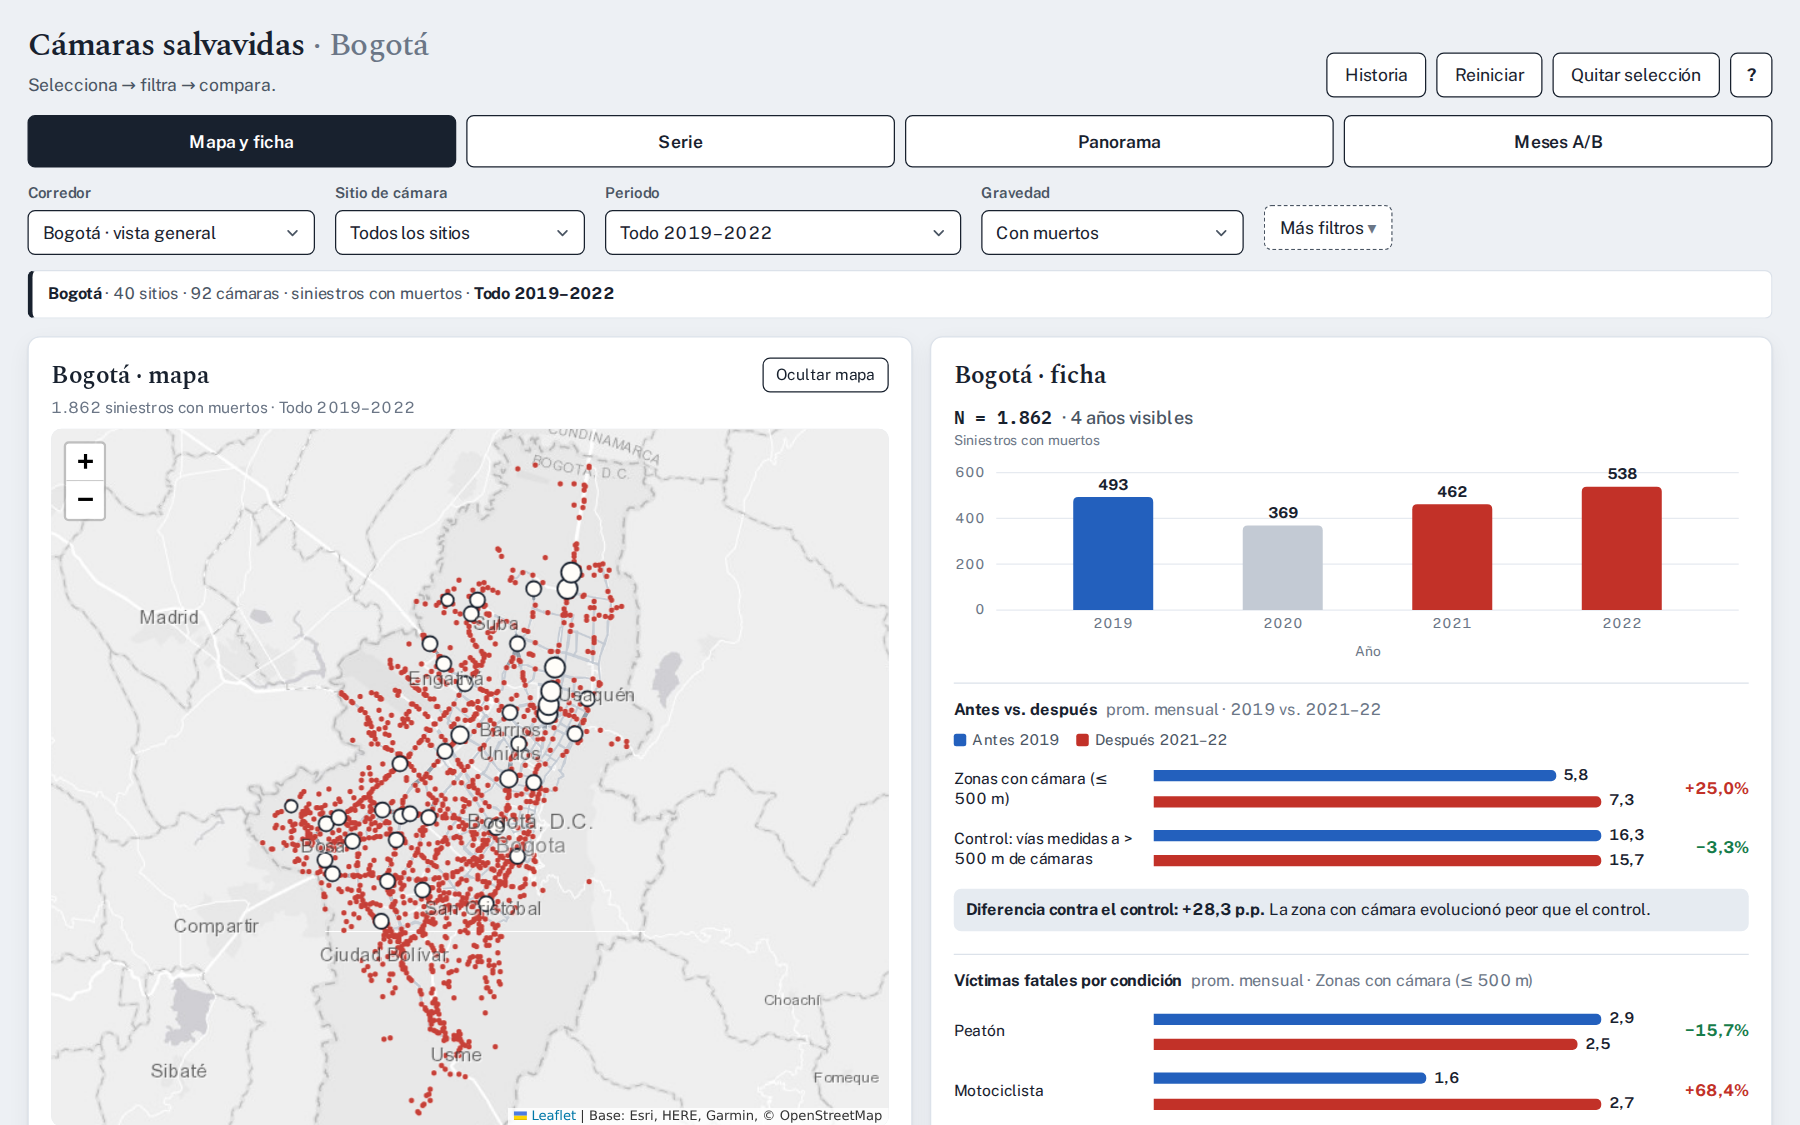
\includegraphics[width=0.49\linewidth]{v2_mapa}\par\smallskip
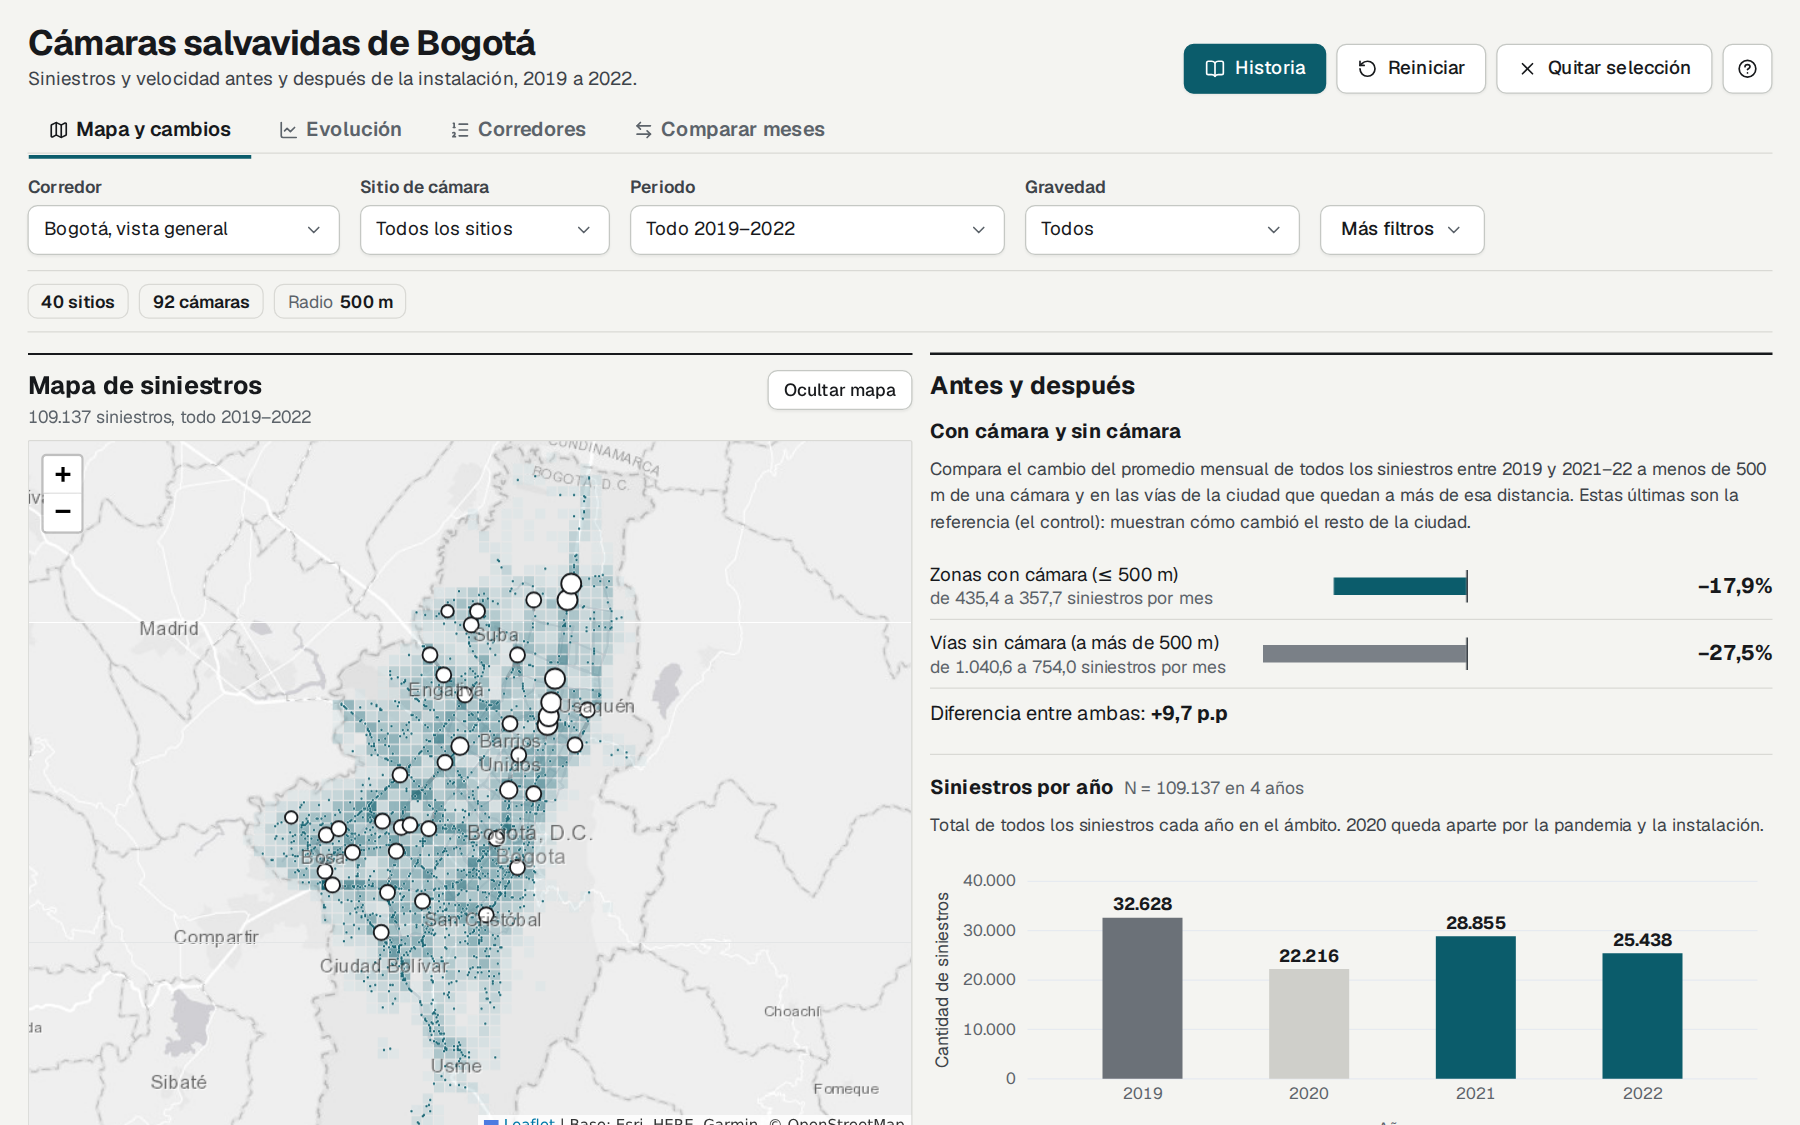
\includegraphics[width=0.49\linewidth]{v3_mapa}\hfill
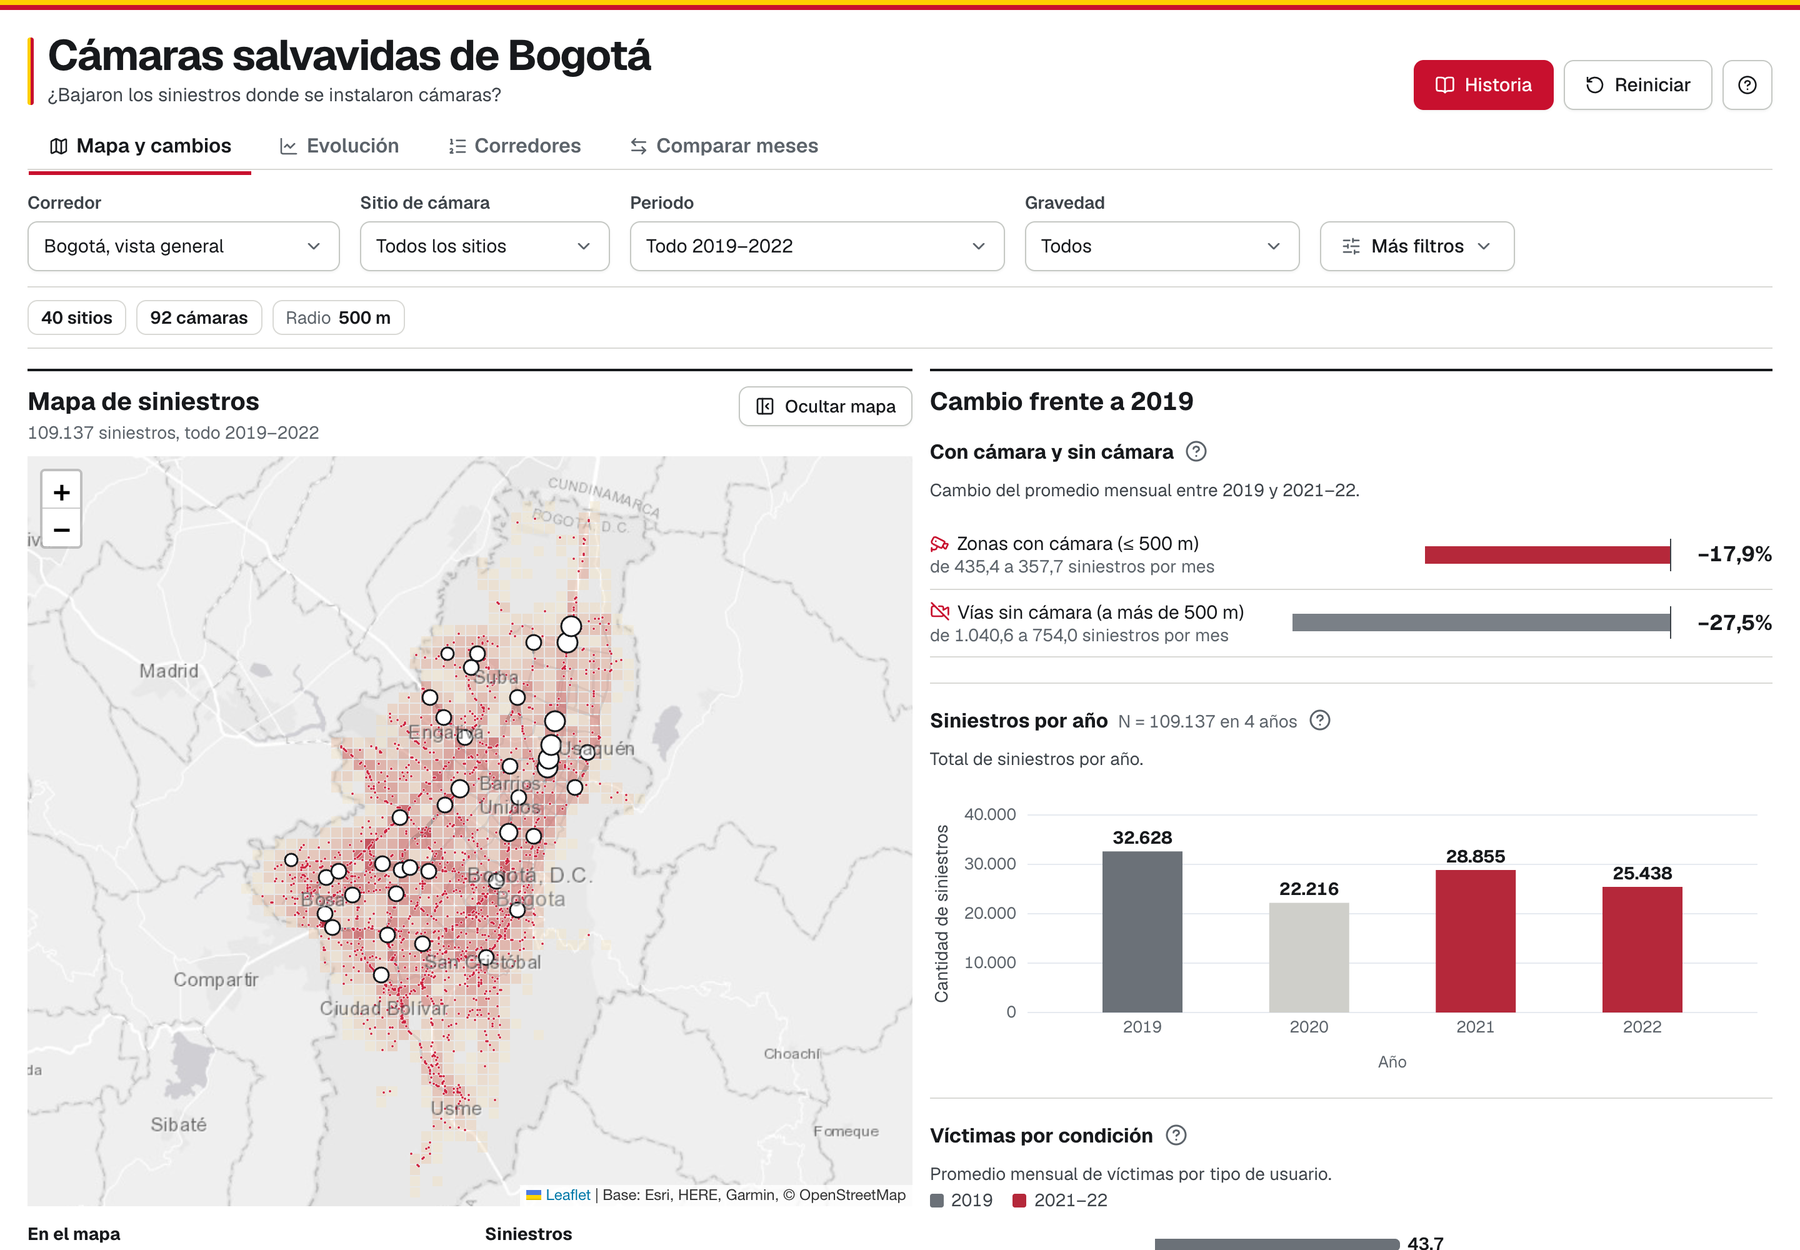
\includegraphics[width=0.49\linewidth]{it3}
\caption{La vista principal en sus cuatro momentos, de izquierda a derecha y de arriba abajo}
\end{figure}

\subsection{Mapa y cambios}

Con 109.137 puntos no se veía ningún patrón, por lo que con poco zoom los agrupamos en celdas de densidad. Para la duda sobre si se tomaba toda la vía o solo un tramo agregamos la casilla ``Visualizar accidentes en corredor'', que muestra toda la vía sin cambiar la comparación con y sin cámara, y dejamos el mapa siempre a la izquierda, sin márgenes y con la opción de ocultarlo. En las vistas donde un filtro no cambia nada dejamos de mostrarlo, porque confundía.


Al principio teníamos barras de antes y después con una escala distinta para cada zona, y el resultado quedaba escondido en una frase. Ahora son dos barras de cambio porcentual sobre una escala común, con las cifras en siniestros por mes y la diferencia escrita debajo, y el periodo elegido actúa como el ``después'' frente a 2019. Además avisamos cuando hay pocos siniestros, mientras que la diferencia que mostramos en \% y es la resta entre los dos cambios, así que no se debe leer como un cambio relativo.

\subsection{Evolución}

La serie existe desde la primera versión, pero entonces era una línea sin una referencia contra la cual juzgar una caída, y la velocidad iba debajo con controles para prender y apagar cada línea. En las versiones siguientes dejamos la instalación y la pandemia siempre visibles, agregamos el promedio de 2019 y quitamos los controles que no aportaban cuando la leyenda ya nombraba las líneas.

\begin{figure}[H]\centering
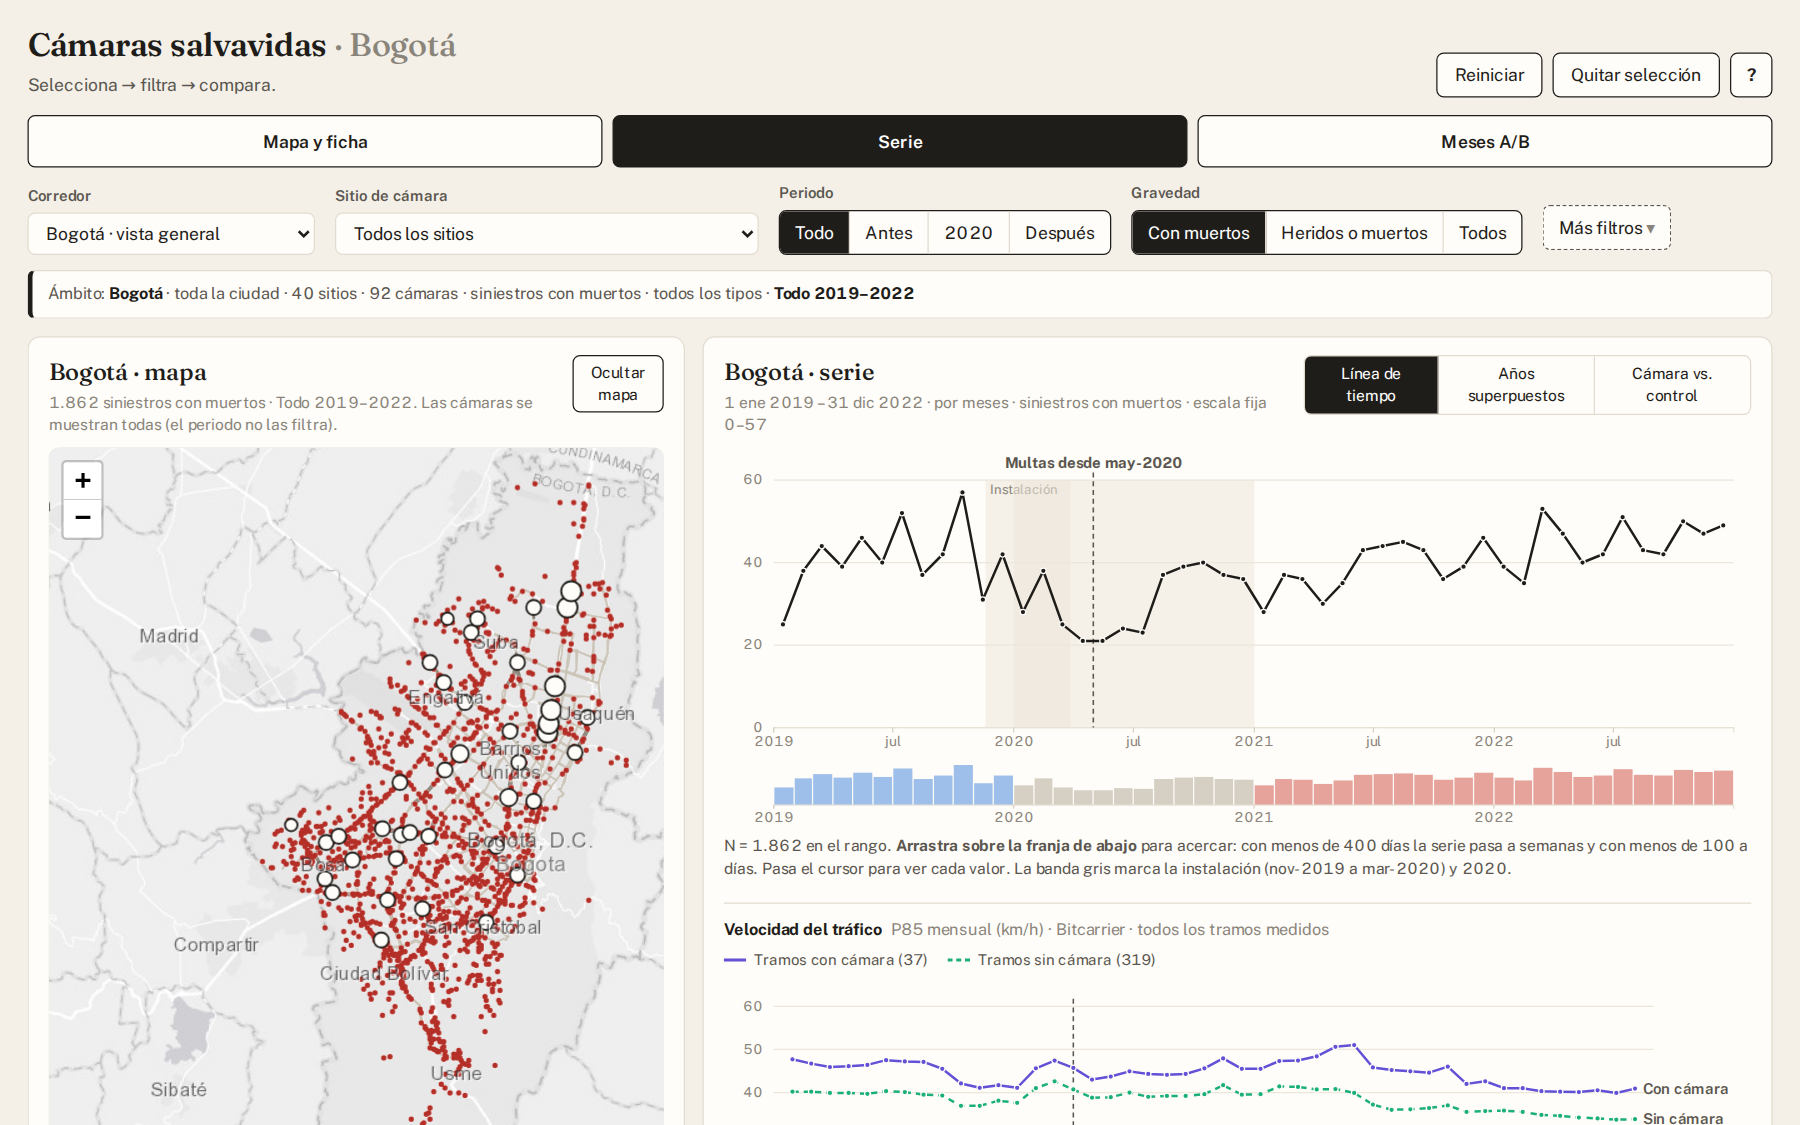
\includegraphics[width=0.325\linewidth,height=0.22\textheight,keepaspectratio]{v1_serie}\hfill
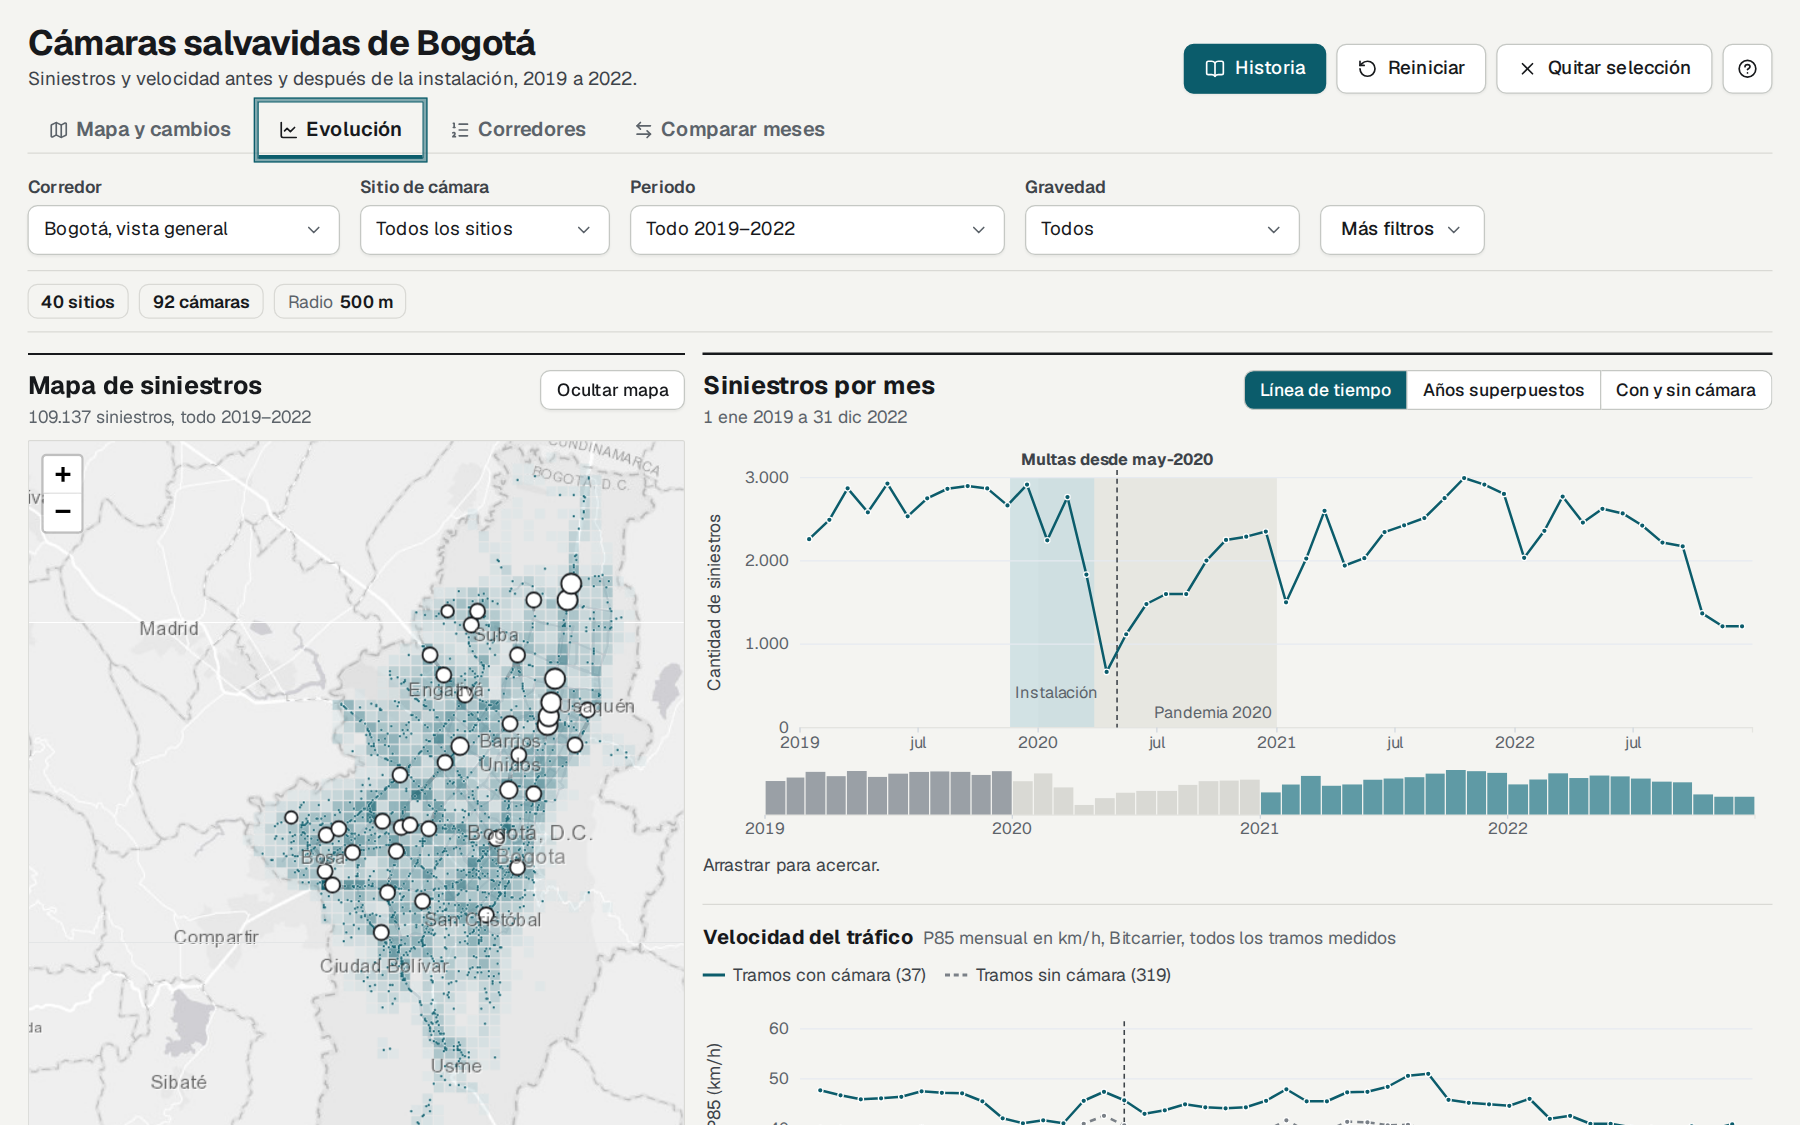
\includegraphics[width=0.325\linewidth,height=0.22\textheight,keepaspectratio]{v3_serie}\hfill
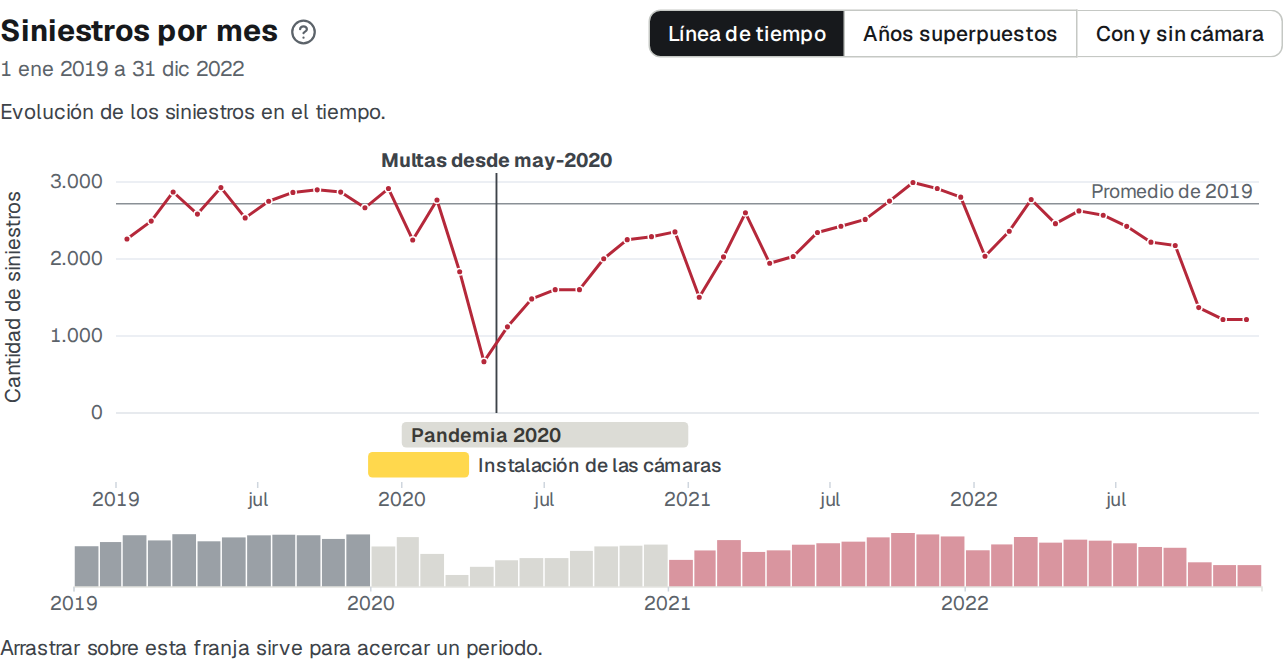
\includegraphics[width=0.325\linewidth,height=0.22\textheight,keepaspectratio]{i_serie}
\caption{La serie en la primera versión, en la tercera y en la actual}
\end{figure}

A la serie le agregamos el promedio de 2019 para poder juzgar las caídas y las recuperaciones, y las cuatro líneas de los años, que se cruzaban, las separamos en recuadros con los mismos colores del resto del dashboard. Las franjas sombreadas de instalación y pandemia tapaban datos y se superponían, así que probamos trazos sobre la gráfica y terminamos con una cinta pegada al eje, siguiendo la idea de dejar el contexto cerca y alineado con los datos.

En la velocidad sumamos la diferencia entre los tramos con y sin cámara en km/h, porque a ojo las dos líneas parecían paralelas, y descartamos otra gráfica de cambio frente a 2019 porque repetía la información. También reescribimos la explicación del P85 para decir que 15 de cada 100 vehículos van más rápido.

\subsection{Corredores}

La vista de corredores nació como Panorama, con un gráfico de mancuernas por gravedad, un diagrama de puntos de los 18 corredores y una dispersión de velocidad, además de un selector de gravedad propio que repetía el filtro global. Varias gráficas respondían lo mismo y ninguna llevaba al detalle de un corredor, por lo que fuimos reduciendo hasta una sola lista ordenable con el detalle al lado.

\begin{figure}[H]\centering
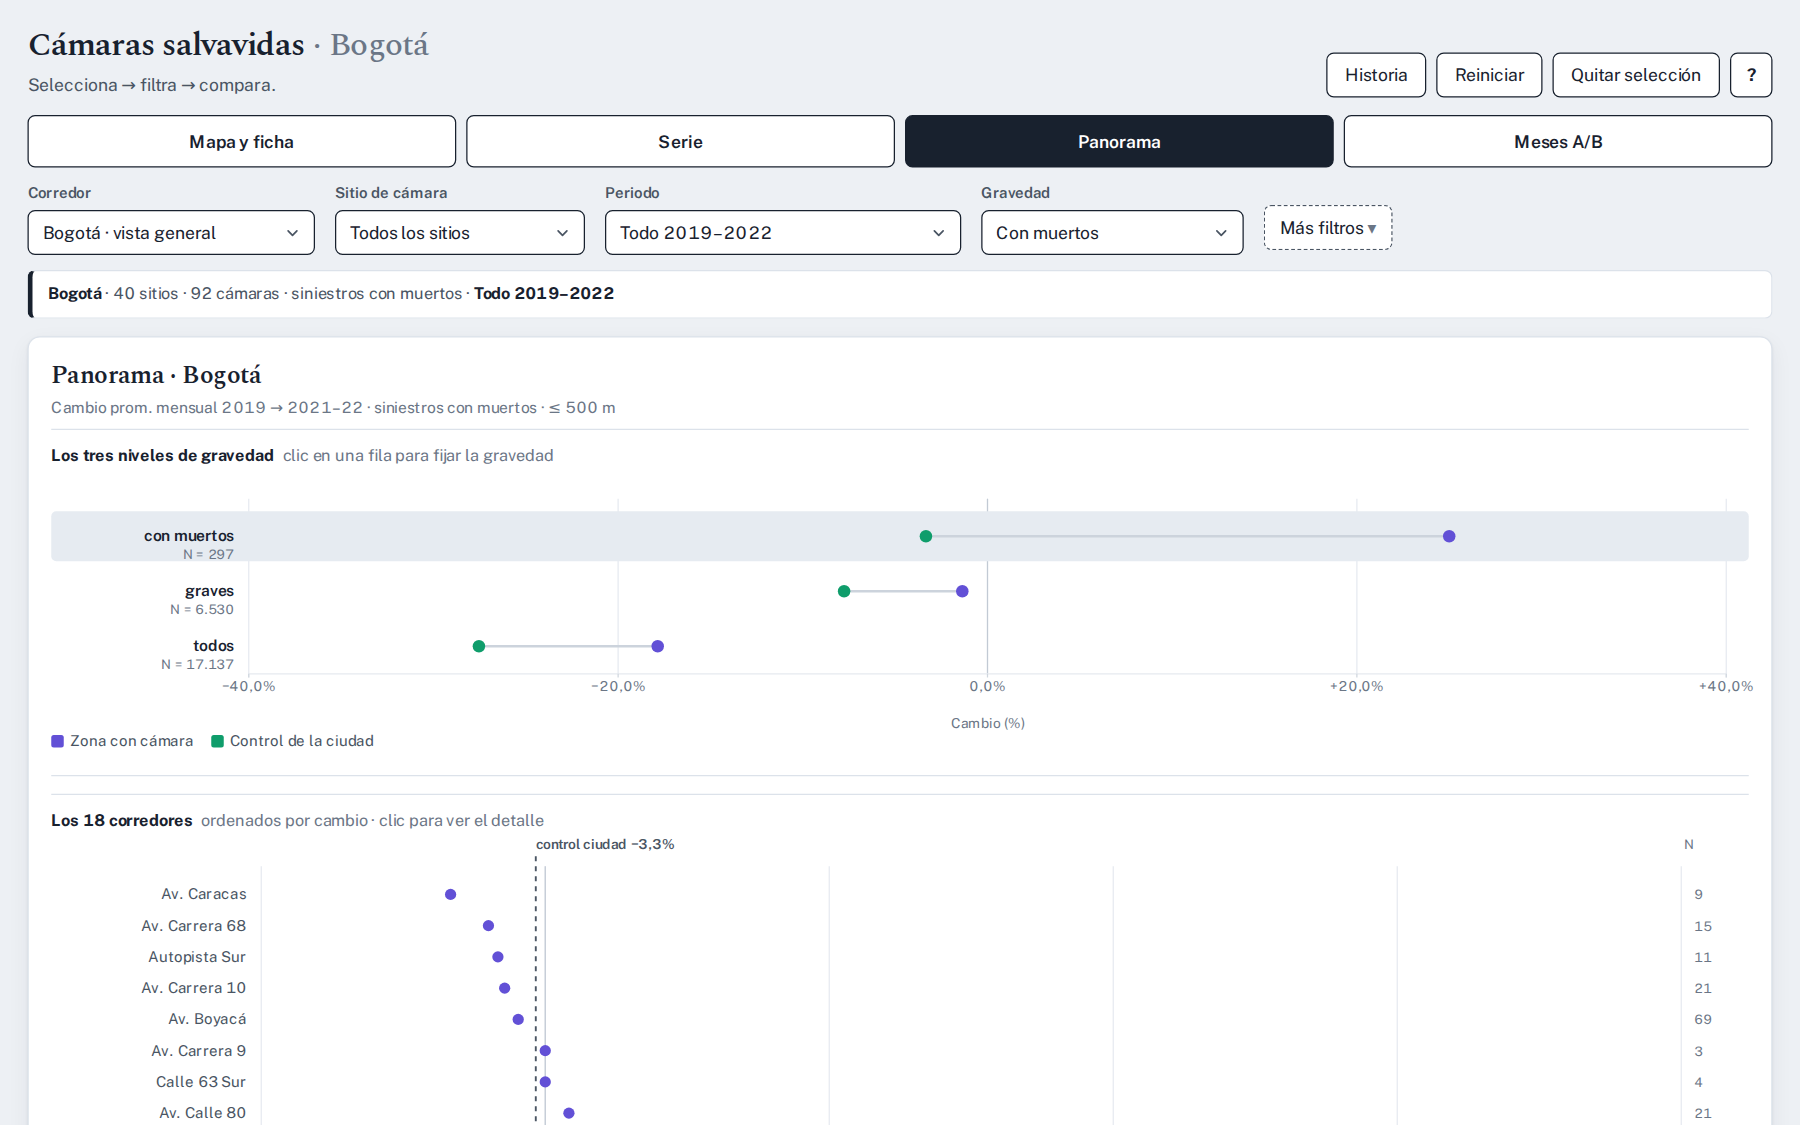
\includegraphics[width=0.325\linewidth,height=0.25\textheight,keepaspectratio]{v2_pan}\hfill
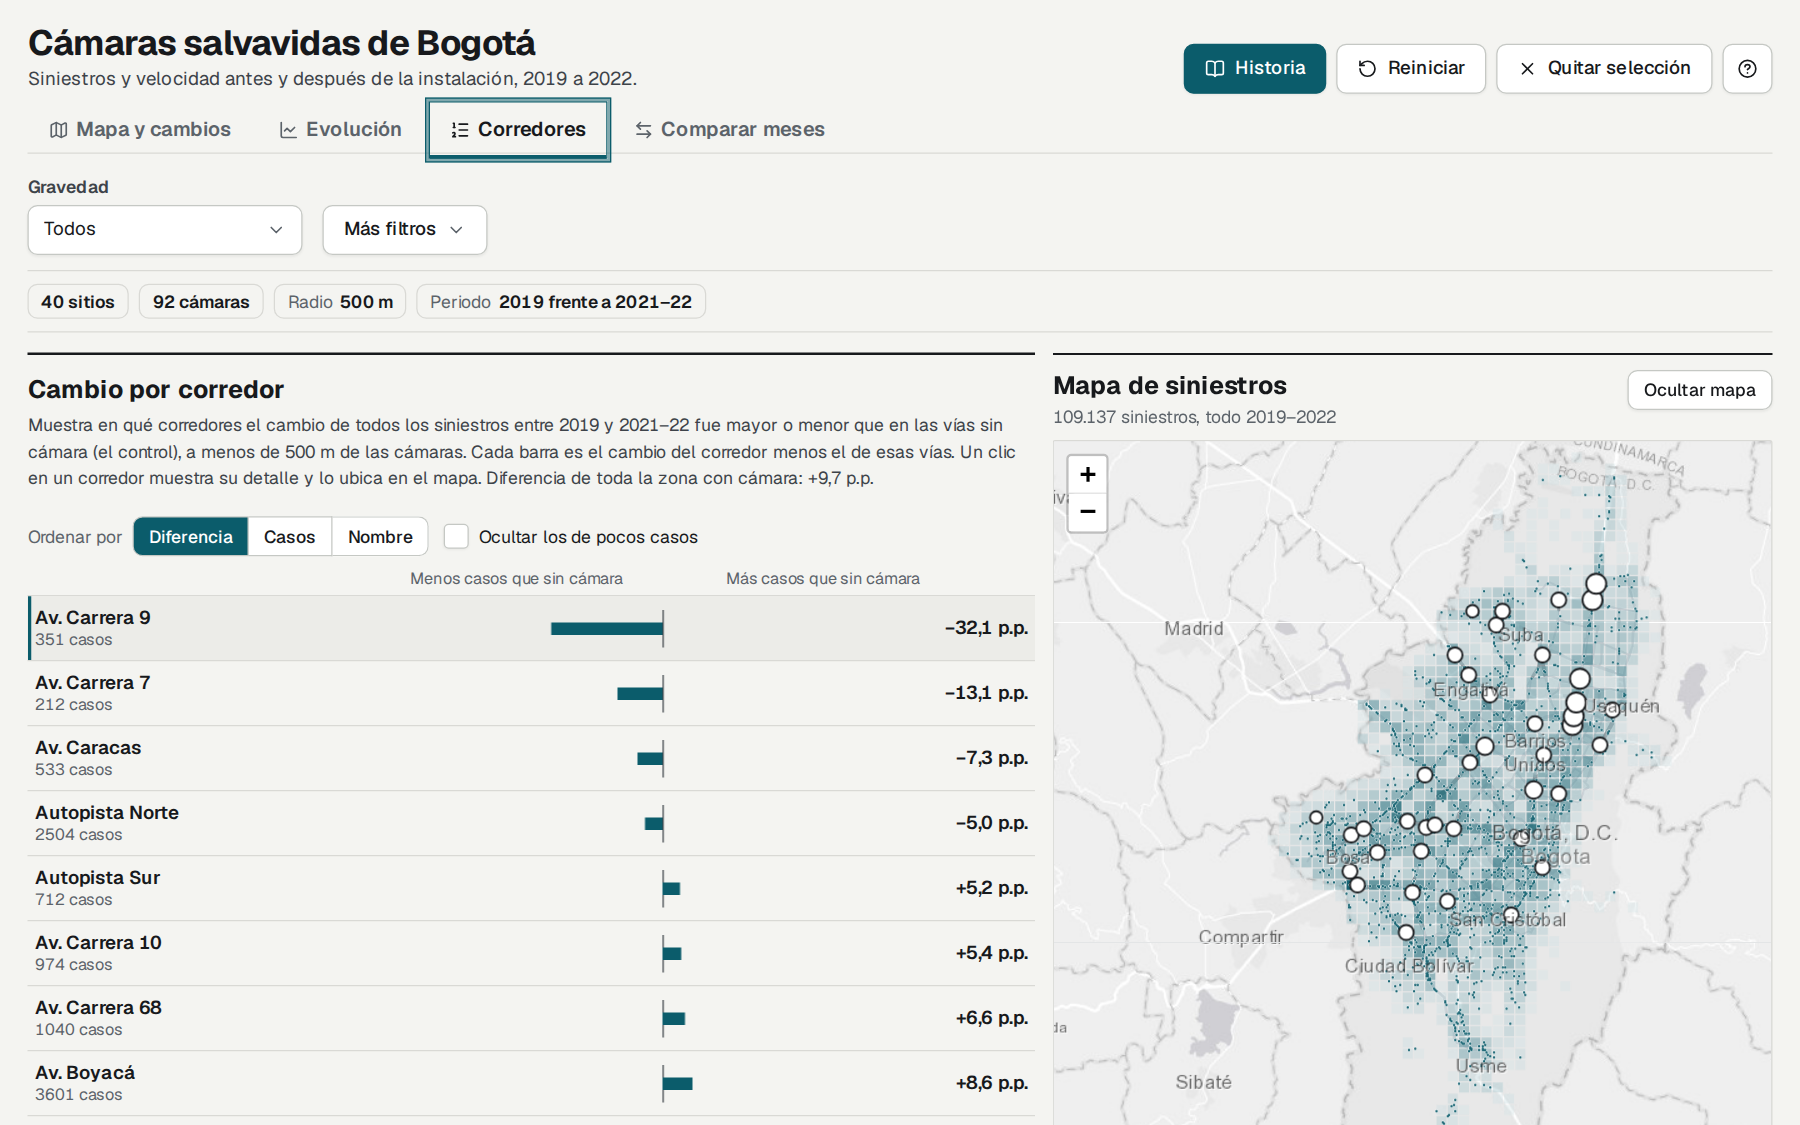
\includegraphics[width=0.325\linewidth,height=0.25\textheight,keepaspectratio]{v3_corr}\hfill
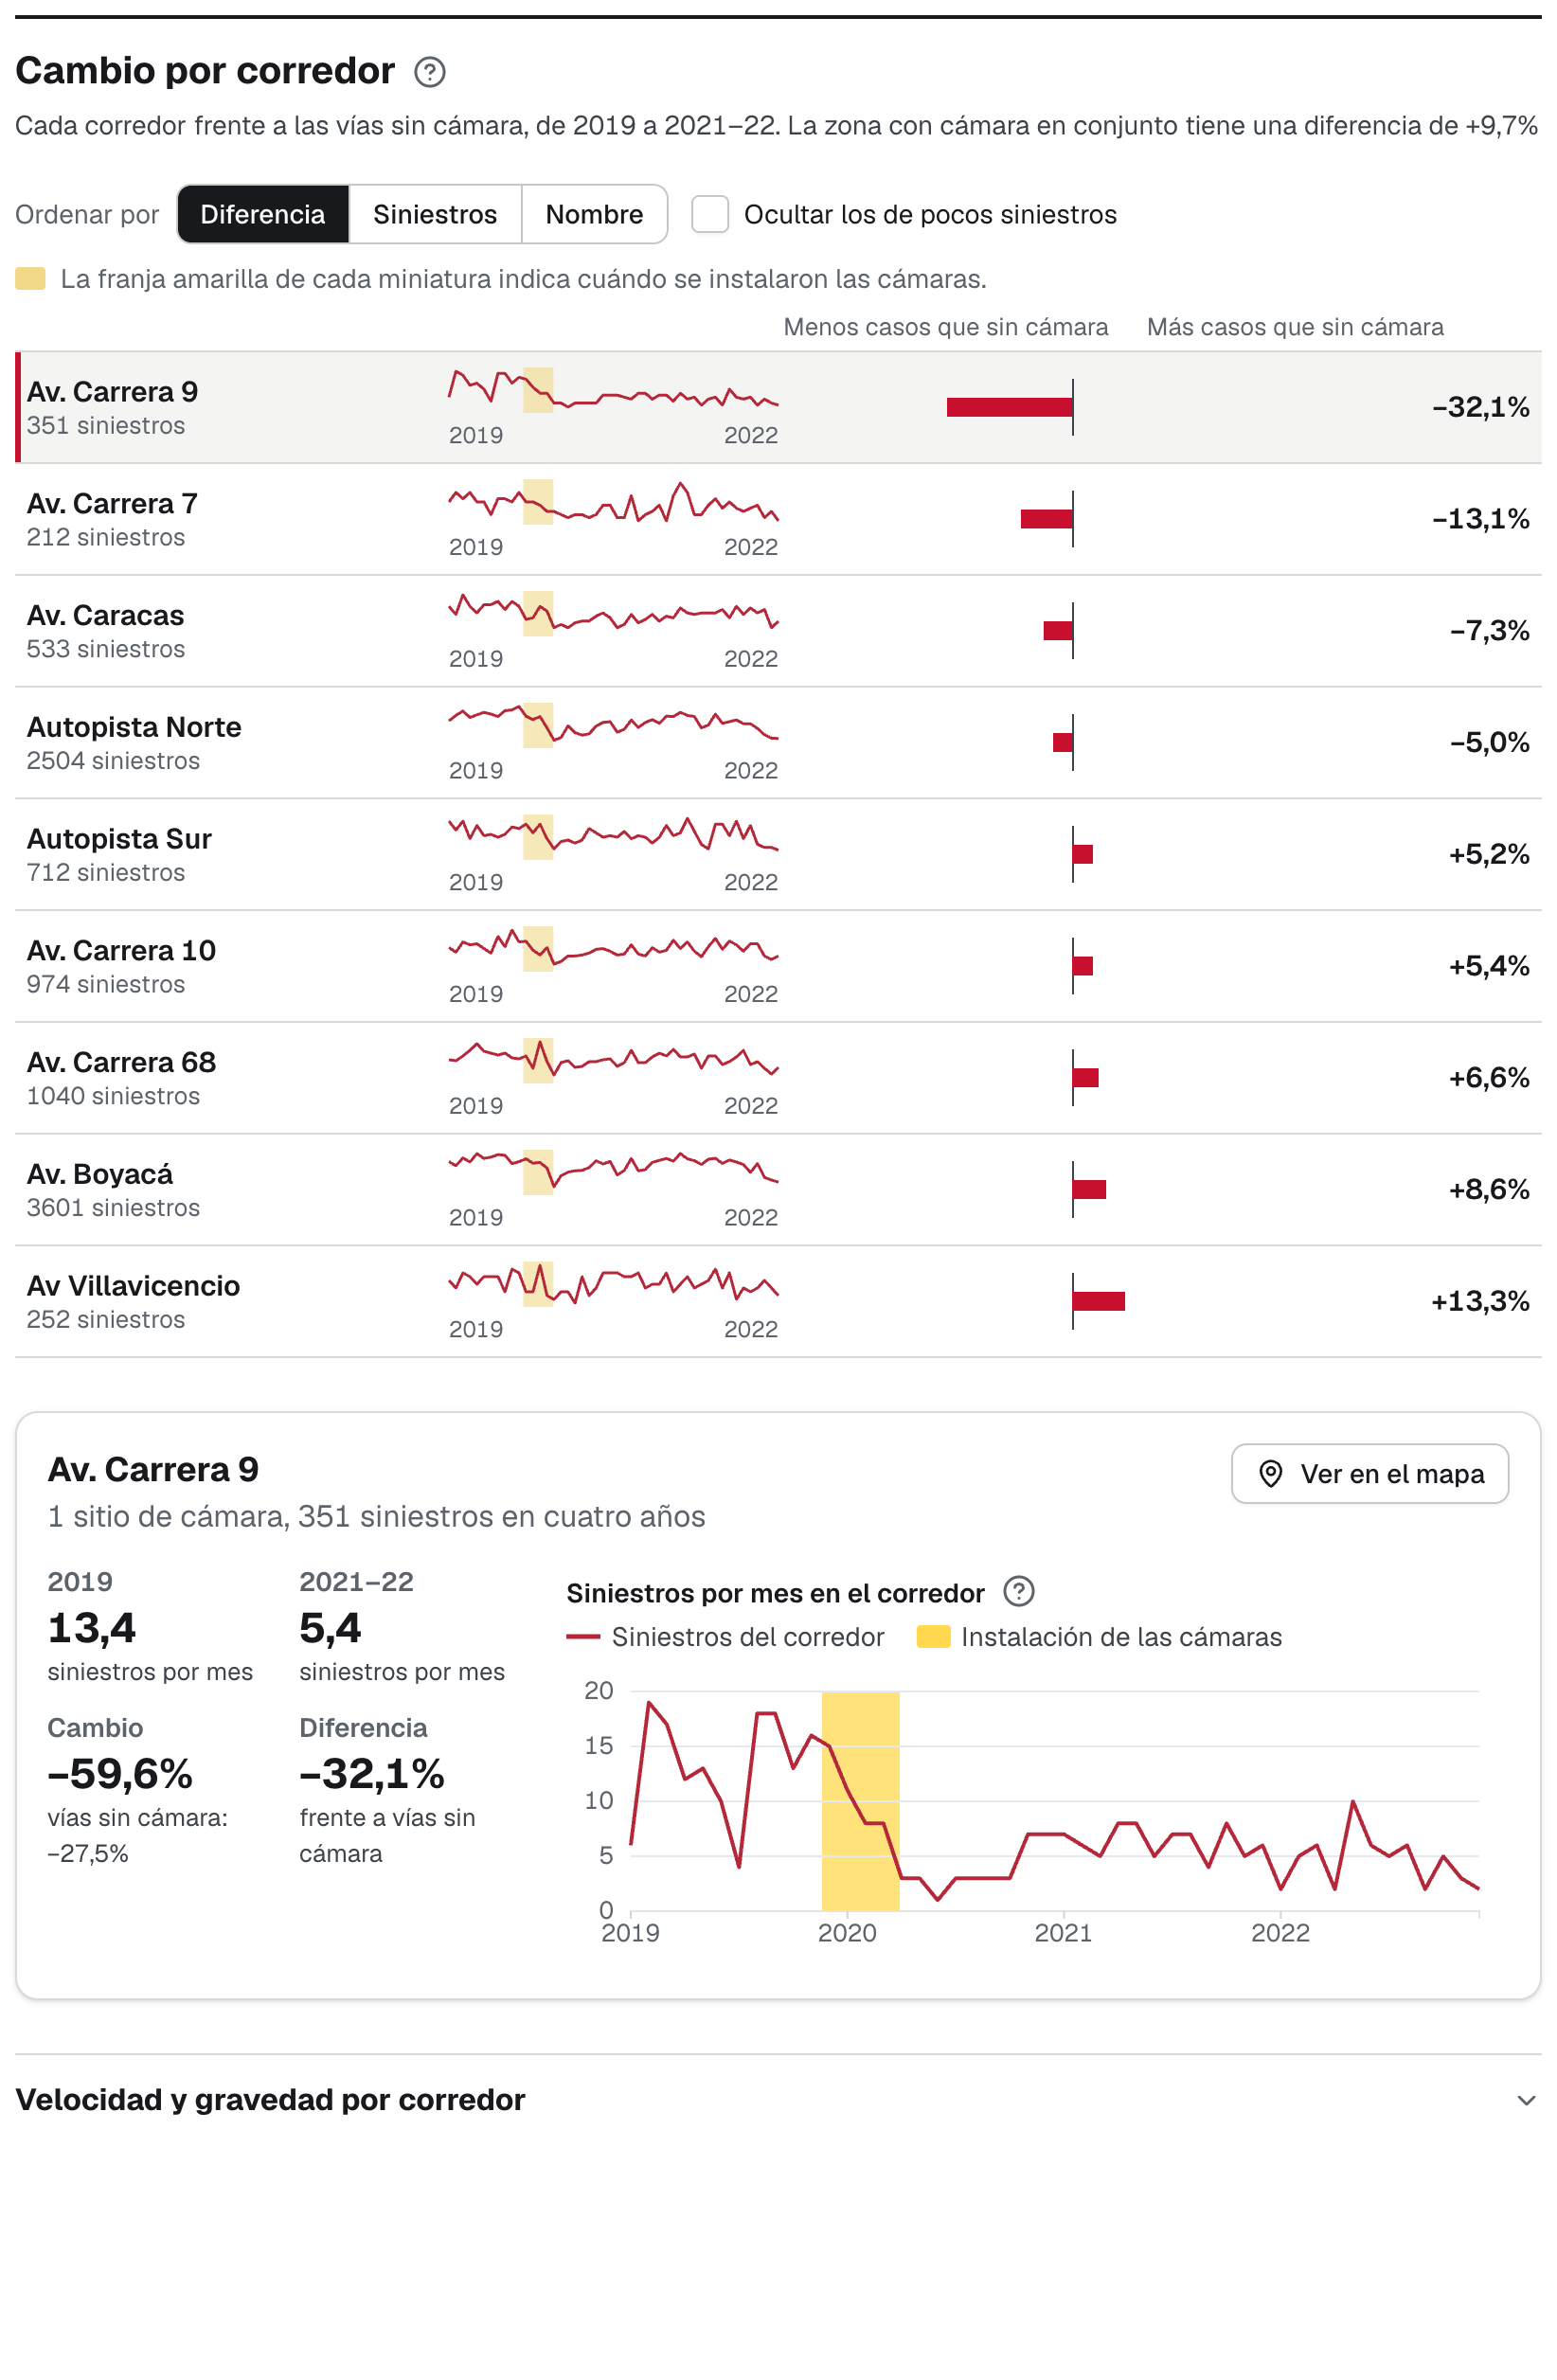
\includegraphics[width=0.325\linewidth,height=0.25\textheight,keepaspectratio]{i_corredores}
\caption{Panorama, la primera lista de corredores y la lista actual}
\end{figure}

Corredores fue la vista que más rediseñamos, ya que en la primera versión varias gráficas respondían lo mismo y el flujo no llevaba a un detalle, así que pasamos a una lista con barras centradas en la referencia, donde un corredor con muy pocos siniestros dominaba la escala. Después pusimos el mapa al lado, enlazado con la lista al pasar el cursor, compactamos el detalle y le agregamos unidades a cada cifra, porque un ``72,6'' suelto no decía qué se contaba, y por último ensanchamos las miniaturas, marcamos los años y la instalación y pusimos una guía en la gráfica de detalle.

Los rótulos del eje pasaron por varias redacciones hasta volver a ``Menos casos que sin cámara'' y ``Más casos que sin cámara'', que fueron los más fáciles de entender aunque en el resto del dashboard hablamos de siniestros. Probamos redacciones con ``reducción'' y con ``bajó más'' o ``bajó menos'', que eran más precisas para los corredores donde los siniestros subieron, pero sonaban raras o había que releerlas, así que preferimos el rótulo corto y dejamos la explicación completa en el icono de ayuda.

\subsection{Comparación de meses}

Comparar meses fue la otra vista que cambió muchas veces, porque la tarea parece sencilla pero pide elegir dos conjuntos de meses, verlos y leer su diferencia sin que ninguna de las tres cosas estorbe a las otras. En la tabla se ve qué problema nos llevó de una versión a la siguiente, hasta quedarnos con una sola forma de seleccionar.

\begin{figure}[H]\centering
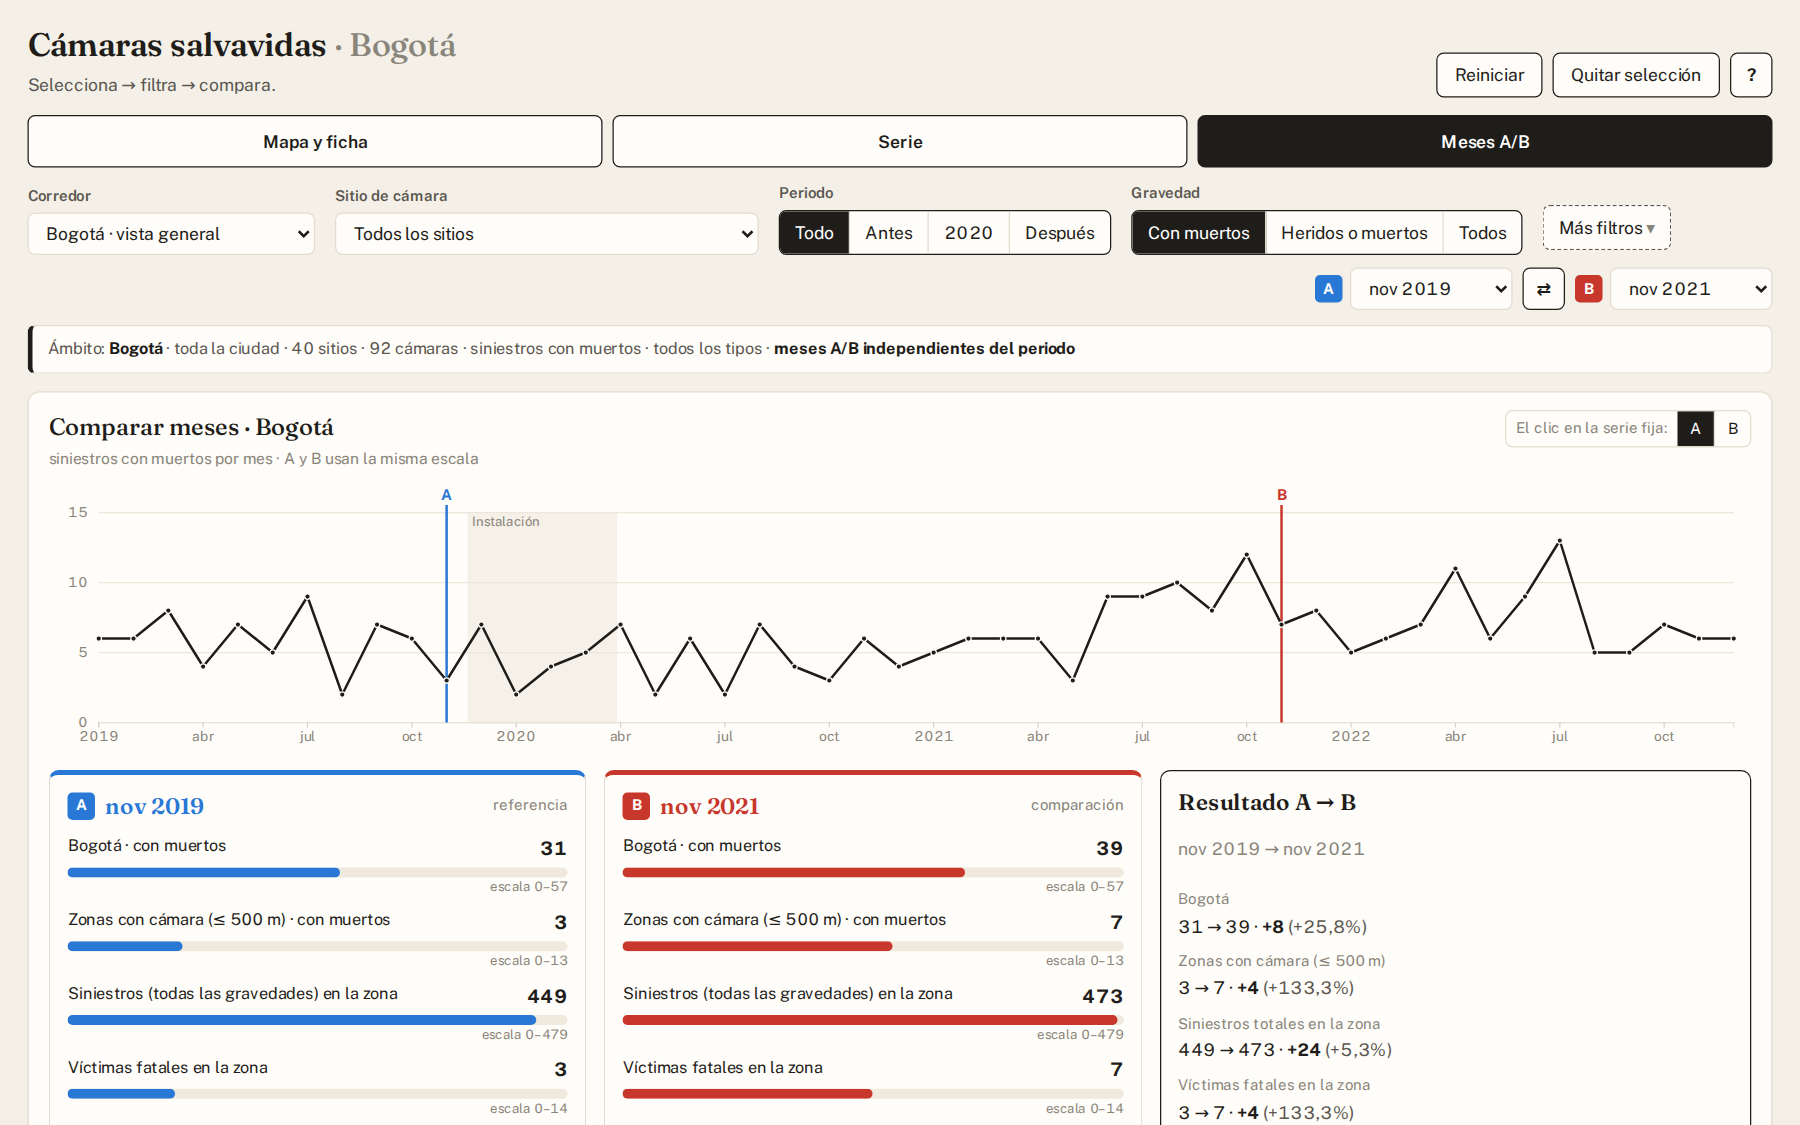
\includegraphics[width=0.325\linewidth,height=0.22\textheight,keepaspectratio]{v1_ab}\hfill
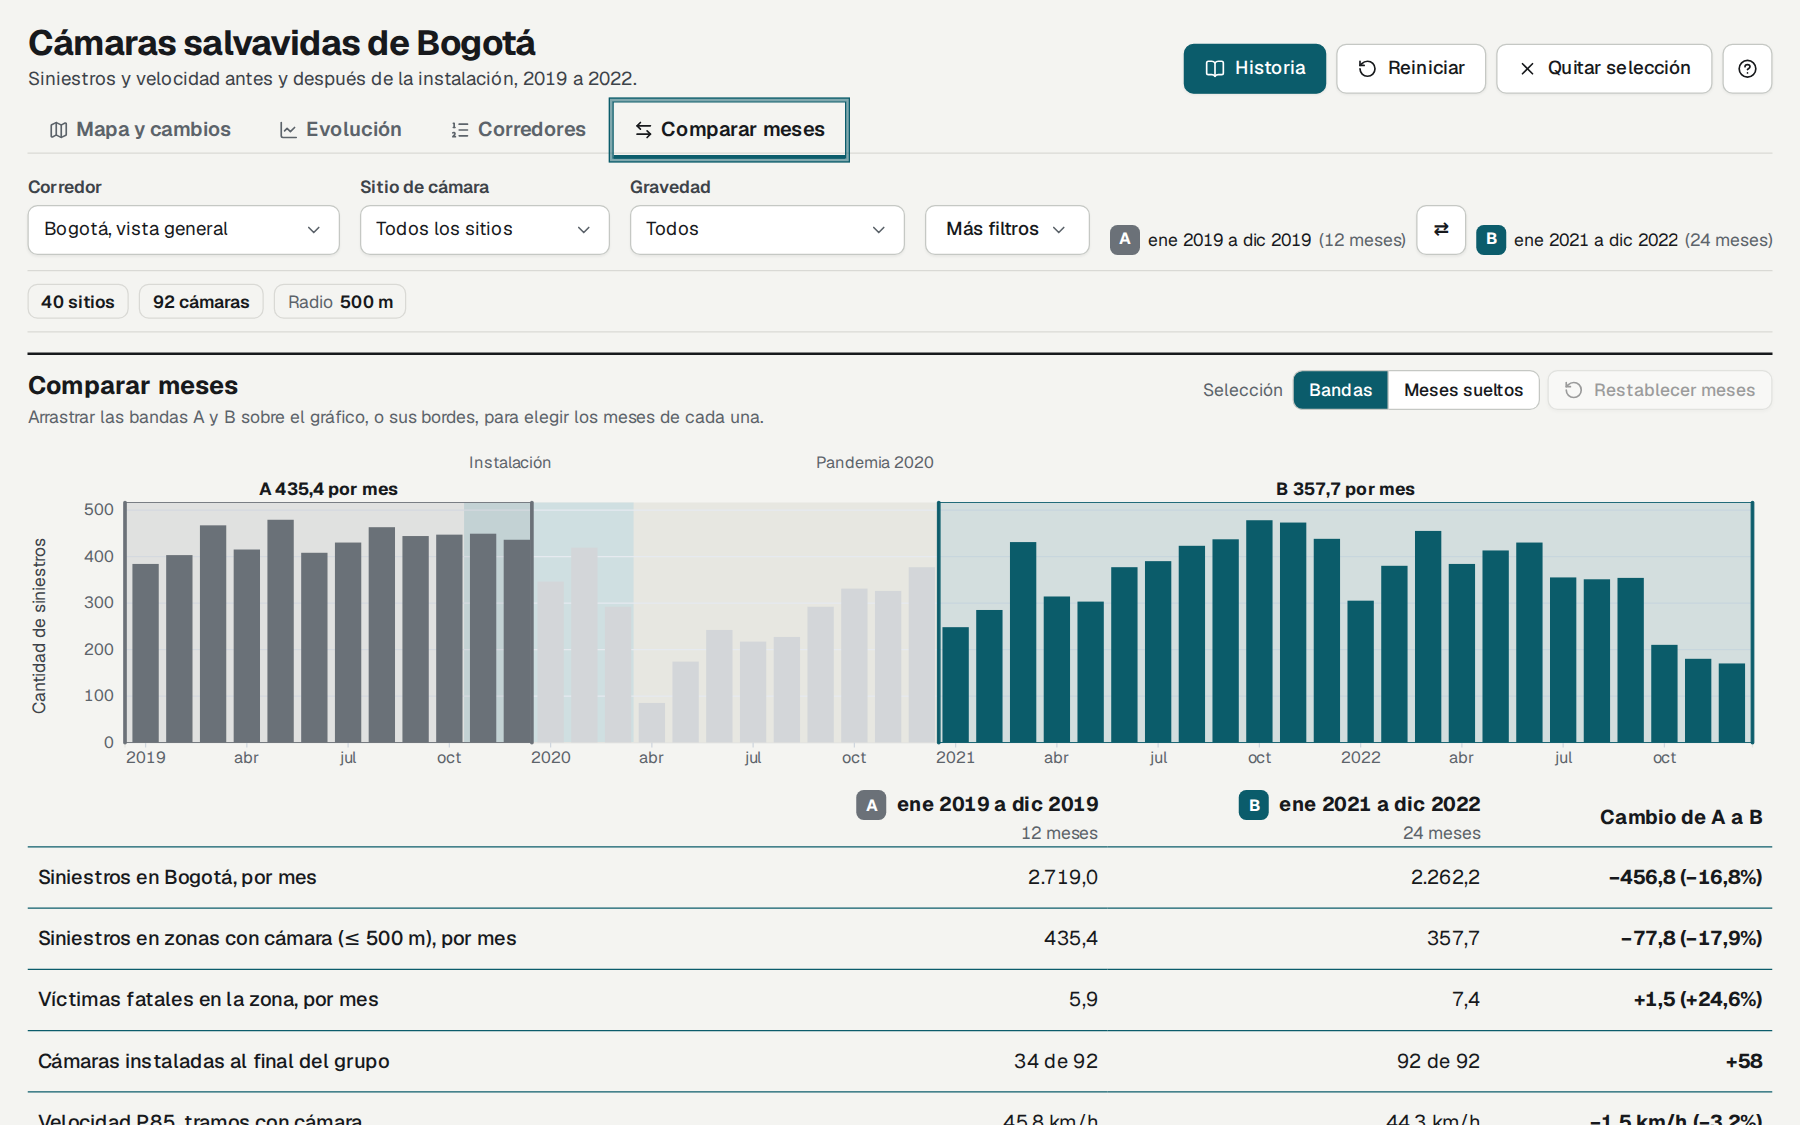
\includegraphics[width=0.325\linewidth,height=0.22\textheight,keepaspectratio]{v3_ab}\hfill
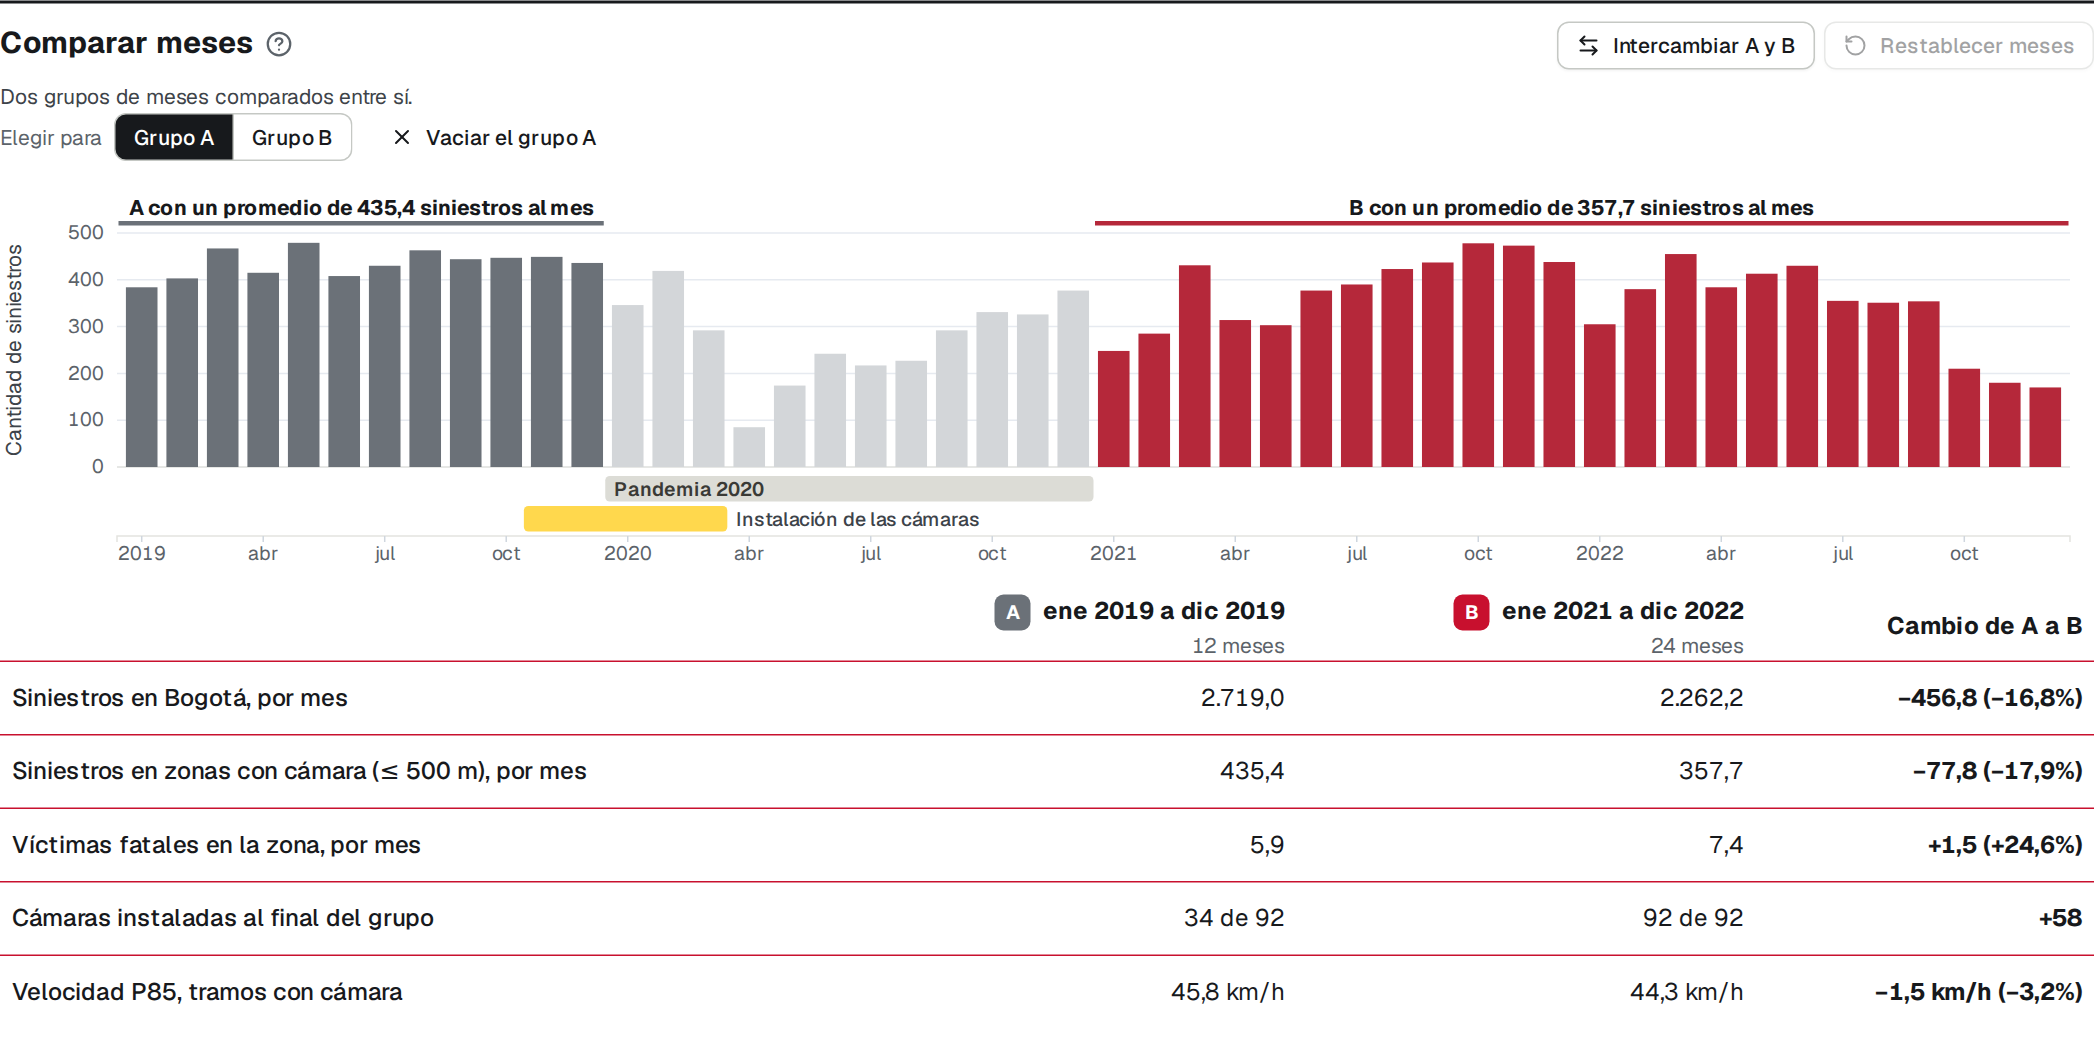
\includegraphics[width=0.325\linewidth,height=0.22\textheight,keepaspectratio]{i_ab}
\caption{Dos meses con tarjetas, bandas arrastrables y grupos de meses}
\end{figure}

\begin{table}[H]\centering\small
\begin{tabularx}{\linewidth}{LL}
\toprule
\textbf{Versión} & \textbf{Problema que llevó al siguiente paso}\\
\midrule
Dos meses sueltos con tarjetas & Mucho texto, y un solo mes tiene mucho ruido.\\
Tabla de A, B y cambio & Poco gráfico.\\
Barras con A y B coloreadas & Las guías punteadas molestaban.\\
Grupos de meses con clic y arrastre & Era un poco complicada.\\
Bandas arrastrables & Manijas pesadas y difícil de restablecer.\\
Bandas o meses sueltos & Dos formas de hacer lo mismo.\\
Actual, solo meses sueltos & Se elige con clic y arrastre y se compara como promedio mensual.\\
\bottomrule
\end{tabularx}
\caption{Recorrido de Comparar meses}
\end{table}

\subsection{Historia y orientación}

La primera versión solo tenía una ayuda para aprender a usar los controles. La historia llegó en la segunda, organizada en tres actos, y cambió varias veces de pasos y de títulos, que al comienzo tenían un tono dramático como ``92 cámaras, 40 sitios, una promesa'' o ``La comparación incómoda''. Los cambiamos por títulos descriptivos porque sonaban a opinión y no a lo que se veía en pantalla. Además, las cifras escritas a mano pasaron a calcularse con los datos y el último paso dejó de devolver el dashboard a como estaba antes de la historia, ya que eso contradecía la idea de abrir la copa a la exploración.

\begin{figure}[H]\centering
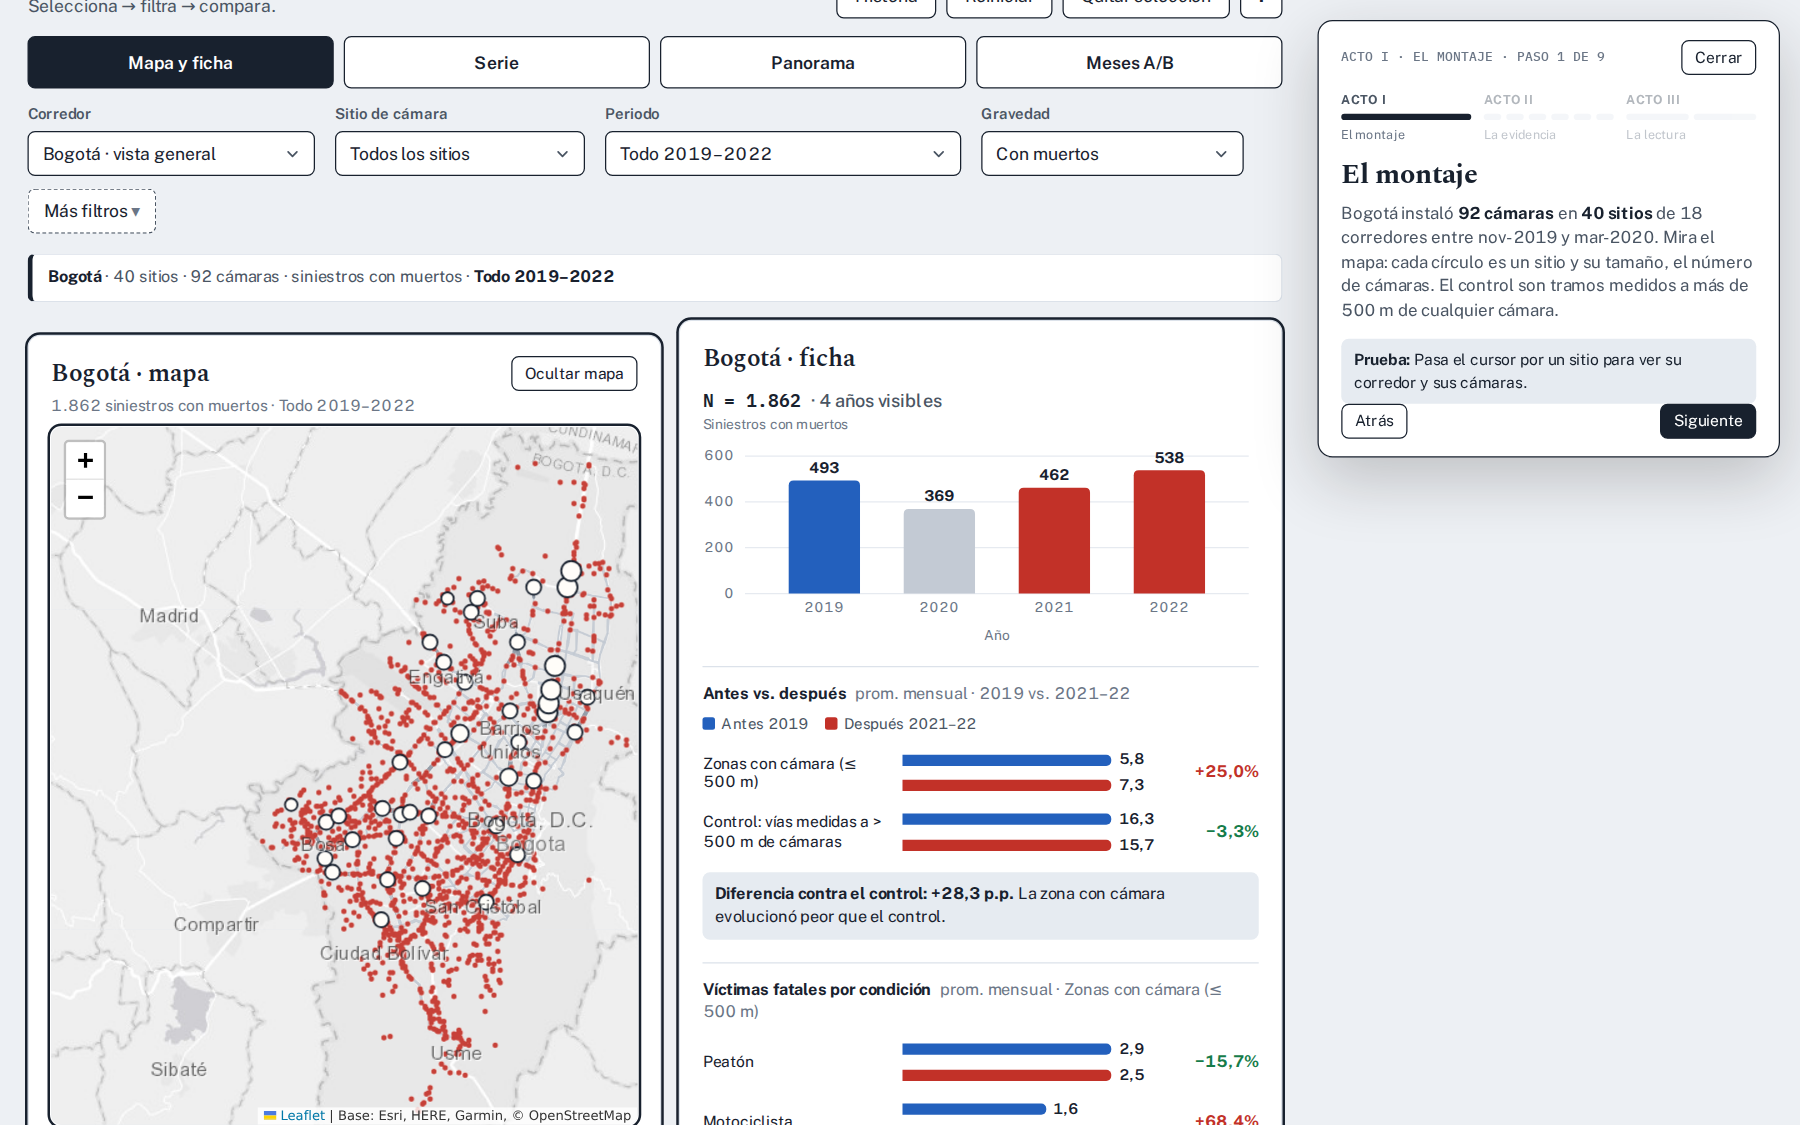
\includegraphics[width=0.49\linewidth,height=0.27\textheight,keepaspectratio]{v2_historia}\hfill
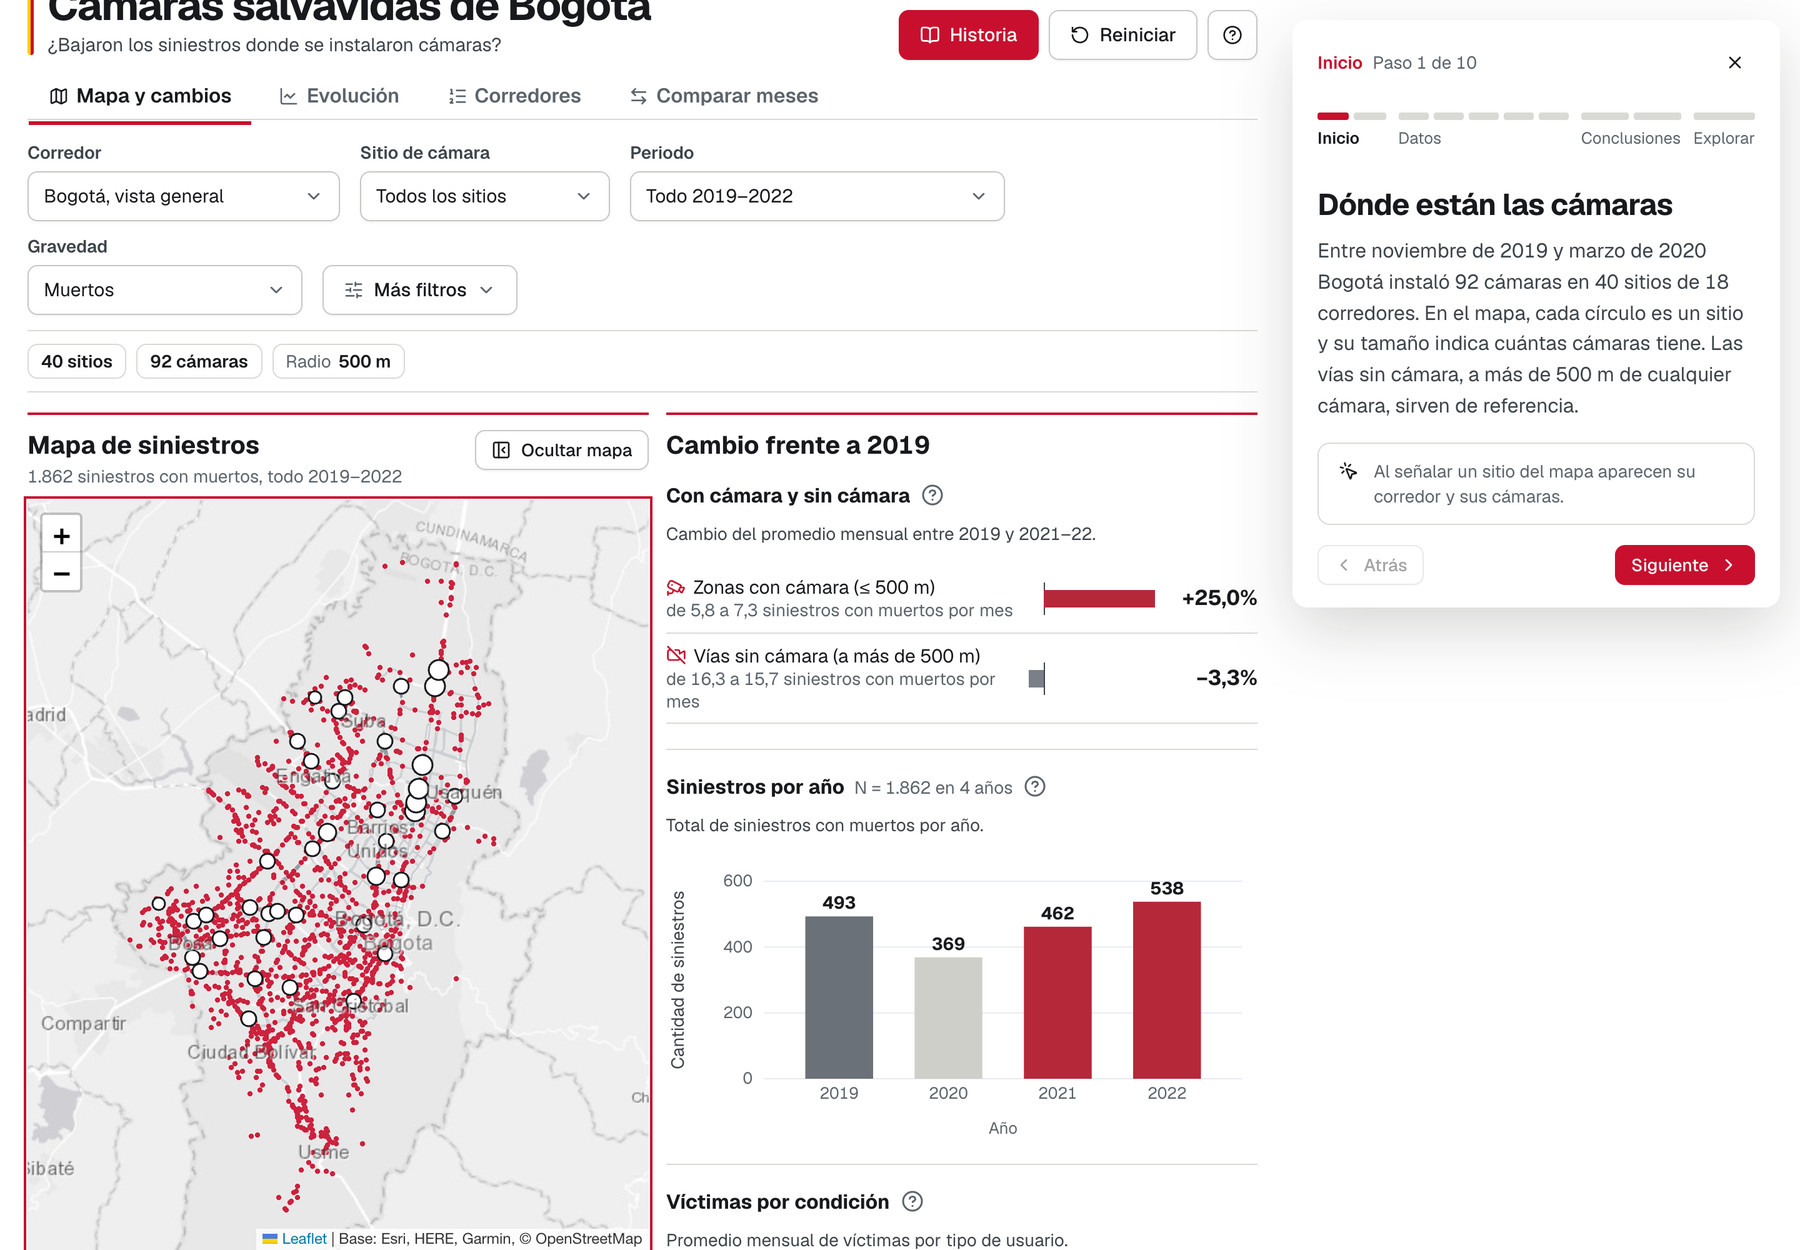
\includegraphics[width=0.49\linewidth,height=0.27\textheight,keepaspectratio]{h1}
\caption{La historia en la segunda versión y en la actual}
\end{figure}

En la misma línea, la pantalla de inicio pasó de un título largo, un párrafo y una lista numerada a mostrar la serie real de la ciudad con una acción principal, y las preguntas, que probamos como una sección fija al final de la página, terminaron en una ventana que se abre desde allí.

\subsection{Identidad, textos y cifras}

Al comienzo había textos de 10 a 12,5 píxeles que costaba leer, así que subimos el mínimo a 13 y dejamos una sola familia sin serifas en lugar de combinar serifas y monoespaciada. En el color pasamos de azul y rojo a un acento verde azulado y finalmente al rojo y amarillo de la bandera de Bogotá sobre fondo blanco, para darle identidad, entendiendo que el rojo señala lo observado y no un juicio.

Como el encabezado se veía genérico, le dimos más peso, una marca con los colores de la bandera y un subtítulo en forma de pregunta. En los iconos nos pasamos al principio, de modo que dejamos solo los que aportan información o ayudan a reconocer una acción, y usamos un mismo kit de componentes, con búsqueda en corredor y sitio, para que todo se comporte igual.

En los textos fuimos cambiando términos y redacción a medida que algo no se entendía o se prestaba para dos lecturas. La regla que terminamos siguiendo es que un mismo concepto se nombra siempre igual y con palabras que usaría cualquiera de los tres perfiles, porque un término técnico o un sinónimo hace pensar que se está hablando de otra cosa.


\begin{table}[H]\centering\small
\begin{tabularx}{\linewidth}{P{4.4cm}P{4.4cm}L}
\toprule
\textbf{Antes} & \textbf{Ahora} & \textbf{Razón}\\
\midrule
``Elige'', ``Haz clic'' & Infinitivos o impersonal & Evitar tutear.\\
``Control'' & ``Vías sin cámara'' & El término era ambiguo.\\
``Casos'' y ``siniestros'' mezclados & ``Siniestros'' & Consistencia.\\
``p.p.'' & ``\%'' & Lectura más sencilla.\\
Descripciones que empezaban con ``Permite'' & Enunciados breves & Es un dashboard y no una guía.\\
Explicaciones largas a la vista & Icono de ayuda & Detalle a demanda, también al tocar.\\
\bottomrule
\end{tabularx}
\caption{Cambios de redacción}
\end{table}


Cada cifra lleva su unidad (``siniestros por mes'' y no un número suelto), usamos la coma decimal y el punto de miles como se escriben en Colombia, un solo decimal en promedios y porcentajes, y el signo en los cambios para saber de un vistazo si algo subió o bajó. En los textos hablamos de que algo cambió y no de que las cámaras lo cambiaron.

\end{document}
